% the tex files from this thesis are from Brendan Duke's Masters thesis: https://github.com/dukebw/master-thesis-fusion

\documentclass[oneside,12pt,oldfontcommands]{memoir}

% Includes
%\usepackage{mathptmx}  % Times New Roman
% \usepackage[T1]{fontenc}
%\usepackage[utf8]{inputenc}
%\usepackage{ebgaramond} % Defines garamond font
% \usepackage[altbullet]{lucidabr}  % Lucida bright
\usepackage{pwuog}  % U of G thesis package

%\input{Nomenclature/nomenclature}
%\nomenclature[1]{$a$}{Vector (including scalars)}%
%\nomenclature[2]{$A$}{Matrix or scalar constant}%
%\nomenclature[3]{$\mathcal{A}$}{Tensor with more than two dimensions}%

% ********************************** Preamble **********************************
% Preamble: Contains packages and user-defined commands and settings
% **************************** Custom Packages ********************************
\let\newfloat\undefined
\usepackage{algorithm}
\usepackage{algpseudocode}
\usepackage{amsfonts}       % blackboard math symbols
\usepackage{amsmath}
\usepackage{amssymb}
\usepackage{bbm}  % for \mathbbm{1}
\usepackage{bibentry}
\nobibliography*
%\newcommand\bmmax{2}
\newcommand\hmmax{0}
\newcommand\bmmax{0}
\usepackage{bm}  % for more powerful bold symbols https://tex.stackexchange.com/a/596
\usepackage{booktabs}
\usepackage{breakcites}
\usepackage{pifont}  % for dingbats checkmark and xmark
\usepackage{mathtools}
\usepackage{ifthen}
\usepackage{keyval}
\usepackage{placeins}
\usepackage{tabu}
\usepackage{tikz}
\usepackage[normalem]{ulem}
\usepackage{upgreek}
\usepackage{natbib}
\usepackage{nicefrac}       % compact symbols for 1/2, etc.
\usepackage{soul}
\usepackage{enumitem}
\usepackage{microtype}      % microtypography
\usepackage{xcolor,colortbl}
\usepackage{tikz}
%\usepackage{subfigure}
\usepackage{tabularx}
\usepackage{makecell}
\usepackage{titlesec}

%for background
%\DeclareMathOperator{\E}{\mathbb{E}}

\usepackage{wrapfig,lipsum,booktabs}

\usepackage{multirow}

\DeclareMathOperator*{\argmax}{argmax}
\DeclareMathOperator{\Tr}{Tr}  % GWT: Trace
\newcommand{\cmark}{\ding{51}}%
\newcommand{\xmark}{\ding{55}}%

\usepackage{capt-of}
\usepackage{times}
\usepackage{epsfig}
\usepackage[export]{adjustbox}  % for adjusting images
\usepackage{xspace}
\usepackage{setspace}
\usepackage{epigraph} 

%\newcommand*{\eg}{e.g.\@\xspace}
%\newcommand*{\ie}{i.e.\@\xspace}
%\newcommand*{\wrt}{w.r.t.\xspace}

% If you comment hyperref and then uncomment it, you should delete
% egpaper.aux before re-running latex.  (Or just hit 'q' on the first latex
% run, let it finish, and you should be clear).
\usepackage[pagebackref=true,breaklinks=true,colorlinks,bookmarks=false]{hyperref}

\usetikzlibrary{arrows.meta, backgrounds, calc, fit, positioning}

\DeclareMathOperator*{\binop}{\oplus}


% *************************** Graphics and figures *****************************

% Uncomment the following two lines to force Latex to place the figure.
% Use [H] when including graphics. Note 'H' instead of 'h'
%\usepackage{float}
%\restylefloat{figure}

\usepackage{caption}
\usepackage{subcaption}

% ********************************** Tables ************************************
\usepackage{booktabs} % For professional looking tables
% \usepackage{multirow}

%\usepackage{multicol}
%\usepackage{longtable}
%\usepackage{tabularx}

\usepackage{graphbox,graphicx}

% *********************************** SI Units *********************************
\usepackage{siunitx} % use this package module for SI units


% ******************************* Line Spacing *********************************

% Choose linespacing as appropriate. Default is one-half line spacing as per the
% University guidelines

% \DoubleSpacing
\setuogspacing{\OnehalfSpacing}
% \SingleSpacing


% ************************ Formatting / Footnote *******************************

% Don't break enumeration (etc.) across pages in an ugly manner (default 10000)
%\clubpenalty=500
%\widowpenalty=500

%\usepackage[perpage]{footmisc} %Range of footnote options


% *****************************************************************************
% *************************** Bibliography  and References ********************

%\usepackage{cleveref} %Referencing without need to explicitly state fig /table

% Add `custombib' in the document class option to use this section

% changes the default name `Bibliography` -> `References'
\renewcommand{\bibname}{References}


% ******************************** Roman Pages *********************************
% The romanpages environment set the page numbering to lowercase roman one
% for the contents and figures lists. It also resets
% page-numbering for the remainder of the dissertation (arabic, starting at 1).

\newenvironment{romanpages}{
  \setcounter{page}{1}
  \renewcommand{\thepage}{\roman{page}}}
{\newpage\renewcommand{\thepage}{\arabic{page}}}


% ******************************************************************************
% ************************* User Defined Commands ******************************
% ******************************************************************************

\makeatletter                  % You do not need to write [htpb] all the time
\renewcommand\fps@figure{htbp} %
\renewcommand\fps@table{htbp}  %
\makeatother                   %

% *********** To change the name of Table of Contents / LOF and LOT ************

%\renewcommand{\contentsname}{My Table of Contents}
%\renewcommand{\listfigurename}{My List of Figures}
%\renewcommand{\listtablename}{My List of Tables}
\DeclarePairedDelimiter\ceil{\lceil}{\rceil}
\DeclarePairedDelimiter\floor{\lfloor}{\rfloor}
\newcommand{\matr}[1]{#1}
\newcommand{\tens}[1]{\mathcal{#1}}
\renewcommand{\vec}[1]{#1}
\newcommand{\vect}[2]{\vec{#1}^{(#2)}}

% Generalized hadamard product fusion
\newcommand{\thetavec}{\ensuremath{\theta}}
\newcommand{\fusop}{\ensuremath{\mathcal{F_{\thetavec}}}}
\newcommand{\mutanfeat}[1]{\ensuremath{\tilde{#1}}}
\newcommand{\m}{\ensuremath{m}}
\newcommand{\n}{\ensuremath{n}}
\newcommand{\q}{\ensuremath{q}}
\renewcommand{\v}{\ensuremath{v}}
\newcommand{\z}{\ensuremath{z}}
%\newcommand{\A}{\ensuremath{A}}
\newcommand{\B}{\ensuremath{B}}
%\renewcommand{\C}{\ensuremath{C}}
\newcommand{\R}{\ensuremath{\mathbb{R}}}
\newcommand{\T}{\ensuremath{\mathcal{T}}}
\newcommand{\Tfibre}{\ensuremath{\T_{i_1 \cdots i_{n - 1} \,:\, i_{n + 1} \cdots i_N}}}
\newcommand{\TsizeIn}[1]{\ensuremath{I_1 \times \cdots \times I_{n - 1} \times #1 \times I_{n + 1} \times \cdots \times I_N}}
\newcommand{\binopb}{\ensuremath{\sideset{}{_b}\binop}}
\newcommand{\binopseq}{\ensuremath{{(\binopb)}_{b = 1}^B}}
\newcommand{\binoppartition}{\ensuremath{{\{\tuckbranch\}}_b}}
\newcommand{\binoppartB}{\ensuremath{\mathbb{B}}}
\newcommand{\binoppartBseq}{\ensuremath{{(\binoppartB_b)}_{b = 1}^B}}
\newcommand{\tuckbranch}{\ensuremath{\T_r^{\q{}\v{}}}}
\newcommand{\hadamardqv}{\ensuremath{N_r\mutanfeat{q} \odot M_r\mutanfeat{v}}}

% SST
%\newcommand{\real}{\mathbb{R}}
\newcommand{\yvosvalG}{68.1}
\newcommand{\davisvalG}{53.2}
\newcommand{\inputvar}{\mathcal{X}}
\newcommand{\outputvar}{\mathcal{Y}}
\newcommand{\vidfeat}{\mathcal{T}}
\newcommand{\objfeat}{\mathcal{R}}
\newcommand{\pixel}{p}
\newcommand{\querytensor}{\mathcal{Q}}
\newcommand{\keytensor}{\mathcal{K}}
\newcommand{\embtensor}{\mathcal{E}}
\newcommand{\valuetensor}{\mathcal{V}}
\newcommand{\objmean}{\mu_o}
\newcommand{\objcov}{\Sigma_o}
\newcommand{\objctx}{\tilde{\mu}_o}
\newcommand{\viddim}{\real{}^{C\times T\times H\times W}}
\newcommand{\softmax}{\mathtt{softmax}}
\newcommand{\yesmark}{\ding{51}}
\newcommand{\nomark}{\ding{55}}
\newcommand{\J}{$\mathcal{J}$}
\newcommand{\F}{$\mathcal{F}$}
%\renewcommand{\G}{\mathcal{G}}
\newcommand{\JandF}{$\mathcal{J} \& \mathcal{F}$}



\newcommand{\A}{\mathbf{A}}
\newcommand{\Lapl}{\mathbf{L}}
\newcommand{\D}{\mathbf{D}}
\newcommand{\G}{\mathcal{G}}
\newcommand{\V}{\mathcal{V}}
\newcommand{\E}{\mathcal{E}}
\newcommand{\Y}{\mathbf{Y}}
\newcommand{\y}{\mathbf{y}}
\newcommand{\X}{\mathbf{X}}
\newcommand{\x}{\mathbf{x}}
\newcommand{\Z}{\mathbf{Z}}
\newcommand{\h}{\mathbf{h}}
% \newcommand{\H}{\mathbf{H}}
\newcommand{\W}{\mathbf{W}}
\newcommand{\w}{\mathbf{w}}
%\newcommand{\R}{\mathbb{R}}
\newcommand{\eg}{\emph{e.g.}\@\xspace}
\newcommand{\ie}{\emph{i.e.}\@\xspace}
\newcommand{\wrt}{\emph{w.r.t.}\@\xspace}
\newcommand{\IID}{\emph{i.i.d.}\@\xspace}
\newcommand{\std}[1]{{\tiny{$\pm$#1}}}

% \newcommand{\cmark}{\ding{51}}%
% \newcommand{\xmark}{\ding{55}}%

\newcommand{\cnns}{CNNs\xspace}
\newcommand{\cnn}{CNN\xspace}
\newcommand{\gnns}{GNNs\xspace} % $\mathcal{G}$\textit{NNs}
\newcommand{\gnn}{GNN\xspace} % $\mathcal{G}$\textit{NN}

\newcommand{\cgshort}{\textsc{CoGen}\xspace}
\newcommand{\cg}{compositional generalization\xspace}
\newcommand{\CG}{Compositional generalization\xspace}

% NeurIPS 2019
\newcommand{\mnistfull}{\textsc{MNIST}\xspace}
\newcommand{\mnist}{\textsc{MNIST-75sp}\xspace}
\newcommand{\colors}{\textsc{Colors}\xspace}
\newcommand{\tri}{\textsc{Triangles}\xspace}
\newcommand{\collab}{\textsc{Collab}\xspace}
\newcommand{\proteins}{\textsc{Proteins}\xspace}
\newcommand{\dd}{\textsc{D\&D}\xspace}
\newcommand{\synthetic}{\colors, \tri~and \mnist\xspace}
\newcommand{\real}{\collab, \proteins~and \dd\xspace}
\newcommand{\wsup}{weakly-supervised\xspace}

% ICCV 2021
\newcommand{\graph}{\mathit{\cal G}}
\newcommand{\pgraph}{\mathit{\hat{\graph}}}
\newcommand{\structn}{\textsc{GraphN}\xspace}
\newcommand{\oracle}{\textsc{Oracle-Zs}\xspace}

\newcommand{\tmin}{t_\mathrm{min}}
\newcommand{\abs}[1]{\left\lvert#1\right\rvert}
\newcommand{\maxi}[1]{\overline{\mathbf{#1}}}
\newcommand{\mini}[1]{\underline{\mathbf{#1}}}
\newcommand{\interval}[2]{\left[\;#1\:,#2\;\right]}
\newcommand{\sumall}{\sum_{i=0}^s}
\newcommand{\sumj}{\sum_{\substack{i = 0\\i \neq j}}^s}
\newcommand{\di}{\sigma^i(\maxi{\boldsymbol\lambda})}
\newcommand{\djj}{\sigma^j(\maxi{\boldsymbol\lambda})}


% NeurIPS 2021
\newcommand{\mad}[1]{{\scriptsize{$\pm$#1}}}
\newcommand{\sem}[1]{{\scriptsize{$\pm$#1}}}
\newcommand{\topacc}[1]{{\scriptsize{/#1}}}
\newcommand{\f}{a}

\newcommand{\nets}{\mathcal{F}}
\newcommand{\domain}{\mathcal{D}}
\newcommand{\neigh}{\mathcal{N}}
%\newcommand{\h}{\mathbf{h}}
\newcommand{\loss}{{\cal L}}
%\newcommand{\w}{\mathbf{w}}

\newcommand{\params}{parameters\xspace}
\newcommand{\net}{architecture\xspace}

\newcommand{\PLH}{{\mkern-0.1mu\times\mkern-0.1mu}}
\newcommand{\ghnbase}{\textsc{GHN-1}\xspace}
\newcommand{\ghnours}{\textsc{GHN-2}\xspace}
\newcommand{\dataset}{\textsc{DeepNets-1M}\xspace}


\newcommand{\iid}{\textsc{ID}\xspace}
\newcommand{\iidtrain}{\textsc{Train}\xspace}
\newcommand{\iidval}{\textsc{Val}\xspace}
\newcommand{\iidtest}{\textsc{Test}\xspace}
\newcommand{\ood}{\textsc{OOD}\xspace}
\newcommand{\wide}{\textsc{Wide}\xspace}
\newcommand{\deep}{\textsc{Deep}\xspace}
\newcommand{\dense}{\textsc{Dense}\xspace}
\newcommand{\bnfree}{\textsc{BN-free}\xspace}

\newcommand{\bp}{\mathbf{p}}
\newcommand{\bt}{\mathbf{t}}
\newcommand{\bv}{\mathbf{v}}
\newcommand{\bw}{\mathbf{w}}
\newcommand{\bx}{\mathbf{x}}
\newcommand{\by}{\mathbf{y}}
\newcommand{\bz}{\mathbf{z}}

%\newcommand{\bm}{\mathbf{m}}
\newcommand{\bn}{\mathbf{n}}
\newcommand{\be}{\mathbf{e}}
\newcommand{\bc}{\mathbf{c}}

% Other stuff
\newcommand{\best}[1]{{\bfseries#1}}
\newcommand{\densepar}[1]{\textbf{#1}}
\newcommand{\apdx}{\textit{Appendix}} 

\definecolor{bad}{gray}{0.85}
%\definecolor{bad}{gray}{0.95}
\definecolor{extreme}{rgb}{0.82,0.82,0.90}
%\definecolor{bad}{rgb}{0.9,0.9,0.9}
\definecolor{good}{rgb}{0.85, 1.0, 0.85}
\newcommand\crule[3][black]{\textcolor{#1}{\rule{#2}{#3}}}

\newcommand\Tstrut{\rule{0pt}{3ex}}         % = `top' strut
\newcommand\Bstrut{\rule[-1.3ex]{0pt}{0pt}}   % = `bottom'

\newcommand\blfootnote[1]{%
  \begingroup
  \renewcommand\thefootnote{}\footnote{#1}%
  \addtocounter{footnote}{-1}%
  \endgroup
}

\newcommand{\venue}[1]{\ul{#1}}
\newcommand{\fig}[1]{Fig.~{#1}}
\newcommand{\secref}[1]{\S~{#1}}

\setsecnumdepth{subsection}

\renewcommand{\toprule}{\Xhline{3\arrayrulewidth} }
\renewcommand{\midrule}{\Xhline{2\arrayrulewidth} }
\renewcommand{\bottomrule}{\Xhline{3\arrayrulewidth} }

\usepackage{stfloats}
\fnbelowfloat % puts footnotes below the bottom floats
\makeatletter
\def\blfootnote{\xdef\@thefnmark{}\@footnotetext}
\makeatother

%\newcommand{\eqref}[]{}

% ********************************* Appendix ***********************************

% The default value of both \appendixtocname and \appendixpagename is `Appendices'. These names can all be changed via:

%\renewcommand{\appendixtocname}{List of appendices}
%\renewcommand{\appendixname}{Appndx}

\usepackage{newtxtext,newtxmath}  % Times New Roman kind of font
%\usepackage{tocloft}

% ************************ Thesis Information & Meta-data **********************
% Thesis title and author information, refernce file for biblatex
% ************************ Thesis Information & Meta-data **********************
%% Subtitle (Optional)
% \subtitle{}

%% The full name of the author
\settitle{Assessing and Improving Generalization in \\ Graph Reasoning and Learning}
\settitleupper{\MakeUppercase{\uogtitle}}
\setauthor{Boris Knyazev}
\setdoctype{Thesis}
%% \masters % going for a Masters degree
\doctors % going for a PhD
\setdefdate{March, 2022}
\setgraddate{March, 2022}
% \setchair{A. Jones}
% this one
\setchairs{A. Jones}{B. Doe} % or this one
\setmembers{C. Smith \\ D. Somebody \\ Some One Else \\ Yet Another}

%% Department (eg. Department of Engineering, Maths, Physics)
% \dept{Department of Engineering}

%% University and Crest
% \university{University of Guelph}
% Crest minimum should be 30mm.
% \crest{\includegraphics[width=0.2\textwidth]{UofGshield}}
%% Use this crest, if you are using the college crest
%% Crest long miminum should be 65mm
%\crest{\includegraphics[width=0.45\textwidth]{University_Crest_Long}}

%% College shield [optional] 
% Crest minimum should be 30mm.
%\collegeshield{\includegraphics[width=0.2\textwidth]{CollegeShields/Kings}}


%% Supervisor (optional)
%\supervisor{Prof. Kenichi Soga}
%% Supervisor Role (optional) - Supervisor (default) or advisor
%\supervisorrole{Advisor: }

%% Advisor (optional)
%\advisor{Prof. Malcolm Bolton}
%% Advisor Role (optional) - Advisor (default) or leave empty
%\advisorrole{Advisor: }


%% You can redefine the submission text:
% Default as per the University guidelines:
% ``This dissertation is submitted for the degree of''
%\renewcommand{\submissiontext}{change the default text here if needed}

%% Full title of the Degree
% \degreetitle{Master of Applied Science}

%% College affiliation (optional)
% \college{Trinity College}

%% Submission date
% Default is set as {\monthname[\the\month]\space\the\year}
% \degreedate{August 2019}

%% Meta information
% \subject{Computer Vision} \keywords{{Deep Learning} {Visual Question Answering} {Fusion} {Multi-modal} {Activity Recognition} {Neural Architecture Search}}


% ******************************** Front Matter ********************************
% left, right margins and textwidth
\setlrmarginsandblock{1in}{1in}{*}
\setulmarginsandblock{1.5in}{1in}{*}
\checkandfixthelayout 

\begin{document}

\maxtocdepth{subsection} % put 3 levels into the ToC

\frontmatter

\thetitlepage
\setulmarginsandblock{1.2in}{1.2in}{*}
\setheadfoot{30pt}{30pt}
\checkandfixthelayout 

% \approvalpage
% % ******************************* Thesis Declaration ***************************

\begin{declaration}

I hereby declare that except where specific reference is made to the work of 
others, the contents of this dissertation are original and have not been 
submitted in whole or in part for consideration for any other degree or 
qualification in this, or any other university. This dissertation is my own 
work and contains nothing which is the outcome of work done in collaboration 
with others, except as specified in the text and Acknowledgements. This 
dissertation contains fewer than 65,000 words including appendices, 
bibliography, footnotes, tables and equations and has fewer than 150 figures.

% Author and date will be inserted automatically from thesis.tex \author \degreedate

\end{declaration}


\uogabstract
%\section*{}
%\uogpapers
\uogdedication{% ******************************* Thesis Dedidcation ********************************

%\begin{dedication}


\begin{vplace}[0.1]


\begin{minipage}[t]{0.5\textwidth}
    \centering
    \par\noindent\rule{0.9\textwidth}{0.4pt} \\
    ``I promise, I'm not going to work tonight,
    I'm going to stay home with you, and \\ we're going to watch Dragon Tales'' \\
    ---\textit{Adam Sandler (Click movie)}
    \par\noindent\rule{0.9\textwidth}{0.4pt} \\
\end{minipage}
    

\vspace{18pt}

Dedicated to my family

\end{vplace}
%\end{dedication}
}
\uogacknowledgements

% *********************** Adding TOC and List of Figures ***********************
% \renewcommand{\cftchapterfont}{\normalfont\sffamily}   
% \renewcommand{\cftsectionfont}{\normalfont\sffamily}   
{
  \hypersetup{linkcolor=black}
  \tableofcontents
  \listoftables
  \listoffigures
}
%\printnomenclature[6em]

%%% if you have more prelim sections, then
%%% \clearpage
%%% \pagestyle{plain}
%%% \prelimtitle{title} text % for each section before main text

% ******************************** Main Matter *********************************
\mainmatter
\pagestyle{uog}

% ABSTRACT is in other/abstract.tex
\chapter{Introduction\label{sec:intro}}


Our world is a complex compositional system, where simple components are used to create more complex ones and all components interact in a non-trivial way. 
One such component are humans, who have a innate ability to accumulate diverse multi-domain knowledge and learn a rich compositional structure of the surrounding world.
This knowledge allows humans to easily solve a plethora of complex tasks. For example, given a static 2D image of a complex dynamic 3D scene, humans are able to recognize objects, their parts, relationships between them, and predict future events in the scene. Humans can even predict a scene's geographical and demographic context and infer abstract properties such as the sentiment of the scene (\fig{\ref{fig:intro_apps}}, a).
Engineering aims to develop systems and algorithms capable of replacing humans in performing such tasks, especially tasks that are repetitive, laborious or dangerous.
In some practical scenarios such as understanding 2D images, these systems are required to recover the original compositional structure from the input recorded by sensors (\fig{\ref{fig:intro_apps}}, a-c). For example, robots or self-driving cars need to detect objects and their relationships from raw pixels or point clouds. In other scenarios the compositional structure is already provided (\eg by another system or human) and algorithms need to reason about the compositional input to make complex higher-level decisions (\fig{\ref{fig:intro_apps}}, d-f). Example tasks include: predicting properties of molecules, predicting future links between people or predicting properties of biological or artificial neural networks.



\begin{figure}[tbhp]
    \vspace{-10pt}
    \centering
    \small
    \setlength{\tabcolsep}{1pt}
    \begin{tabular}{>{\centering\arraybackslash}p{0.44\textwidth}>{\centering\arraybackslash}p{0.54\textwidth}}
        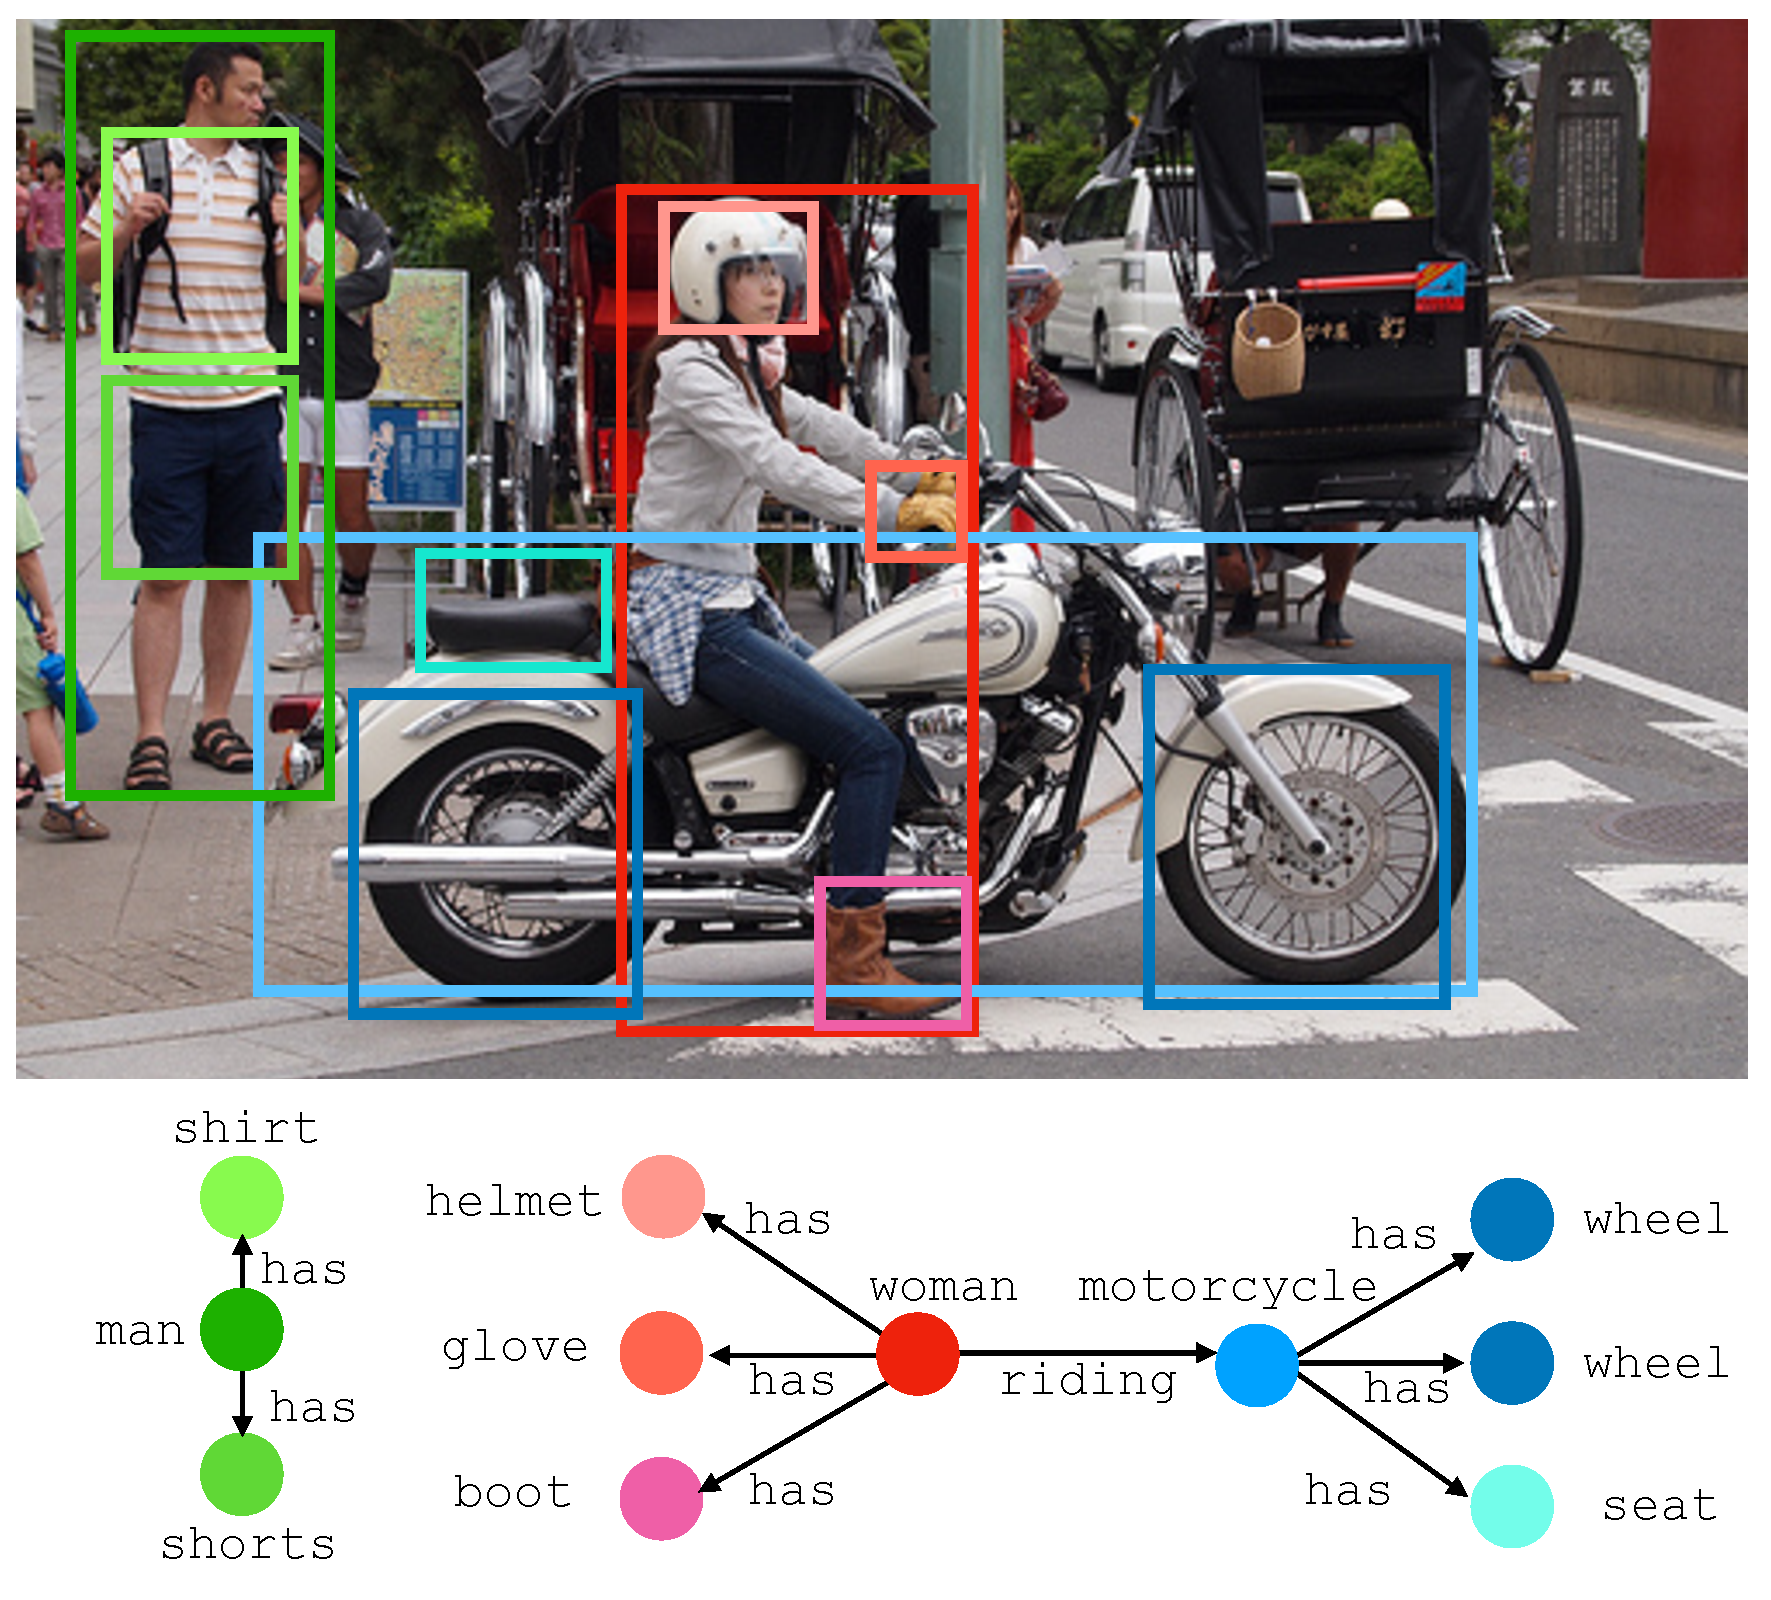
\includegraphics[width=0.3\textwidth, align=c]{Ch1_Intro/motifs_scene_graph.pdf} & {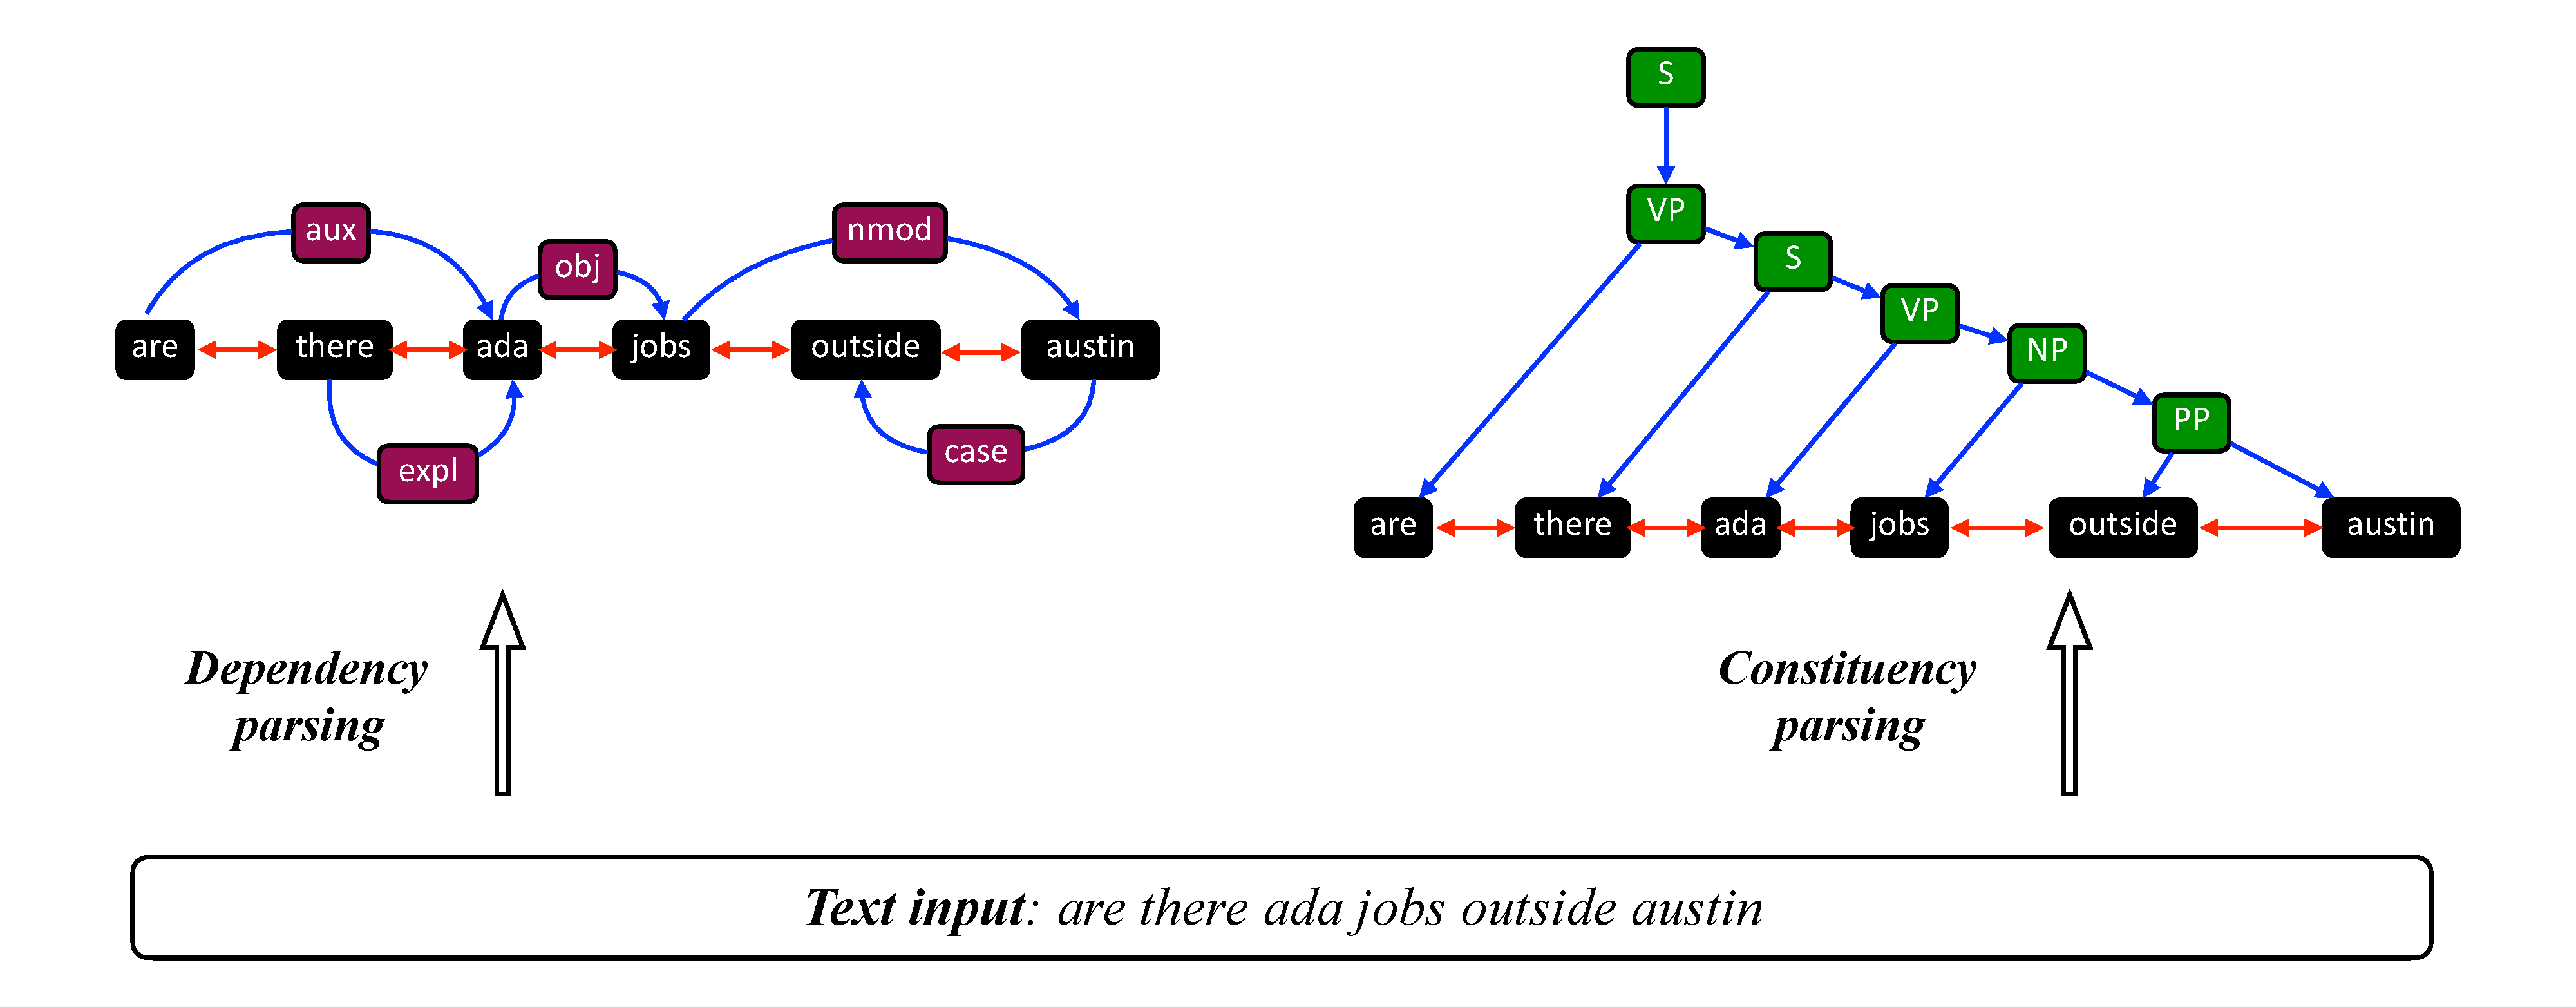
\includegraphics[width=0.53\textwidth, align=c,trim={2cm 12.5cm 36cm 5cm},clip]{Ch1_Intro/graph-construction-v1.pdf}} \\
        (a) Detecting objects and their relationships in a scene~\citep{zellers2018neural} & (b) Modeling language as graphs~\citep{wu2021graph} \\ \\
        
        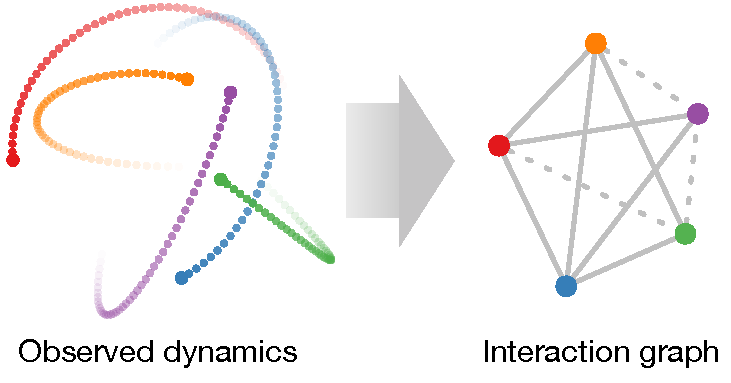
\includegraphics[width=0.35\textwidth, align=c]{Ch1_Intro/nri_physics_graph.pdf} & 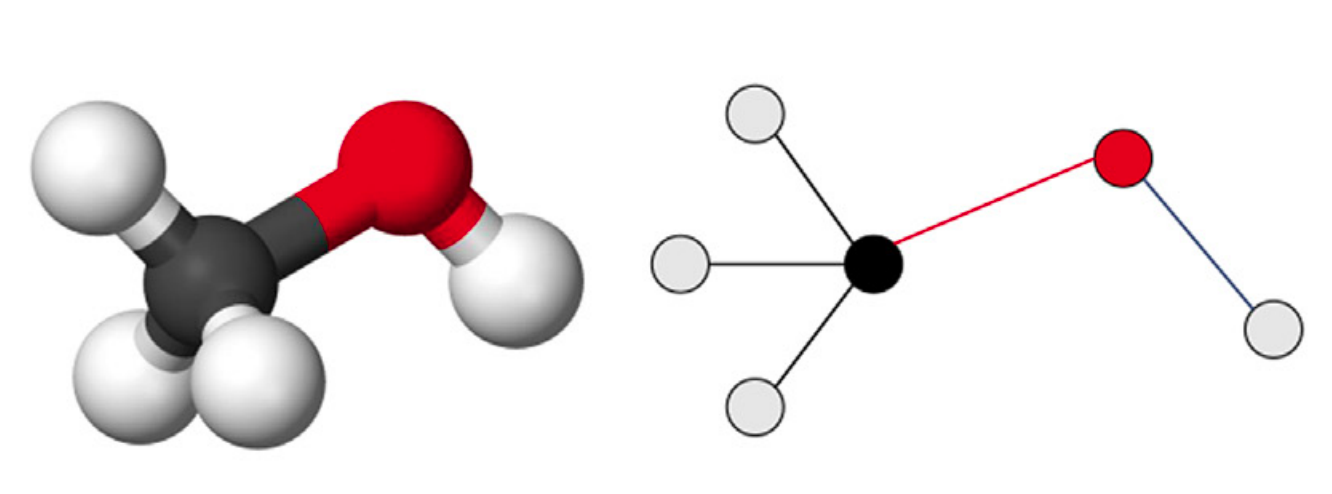
\includegraphics[width=0.5\textwidth, align=c]{Ch1_Intro/molecule_graph.png} \\
        (c) Inferring interactions in physical systems~\citep{kipf2018neural} & (d) Analyzing molecules~\citep{zhou2020graph} \\ \\
        
        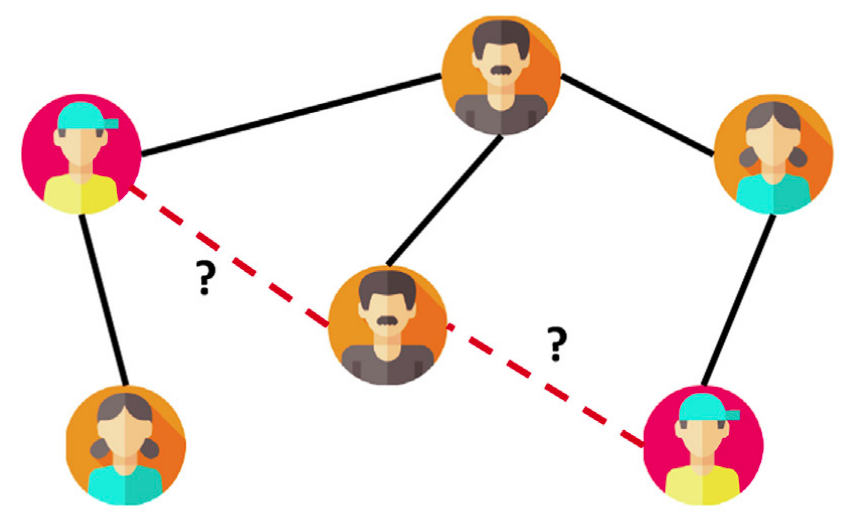
\includegraphics[width=0.3\textwidth, align=c]{Ch1_Intro/fig1_c2.png} & 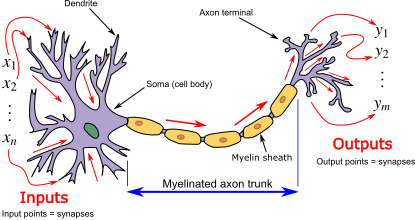
\includegraphics[width=0.3\textwidth, align=c]{Ch1_Intro/Neuron3.png} 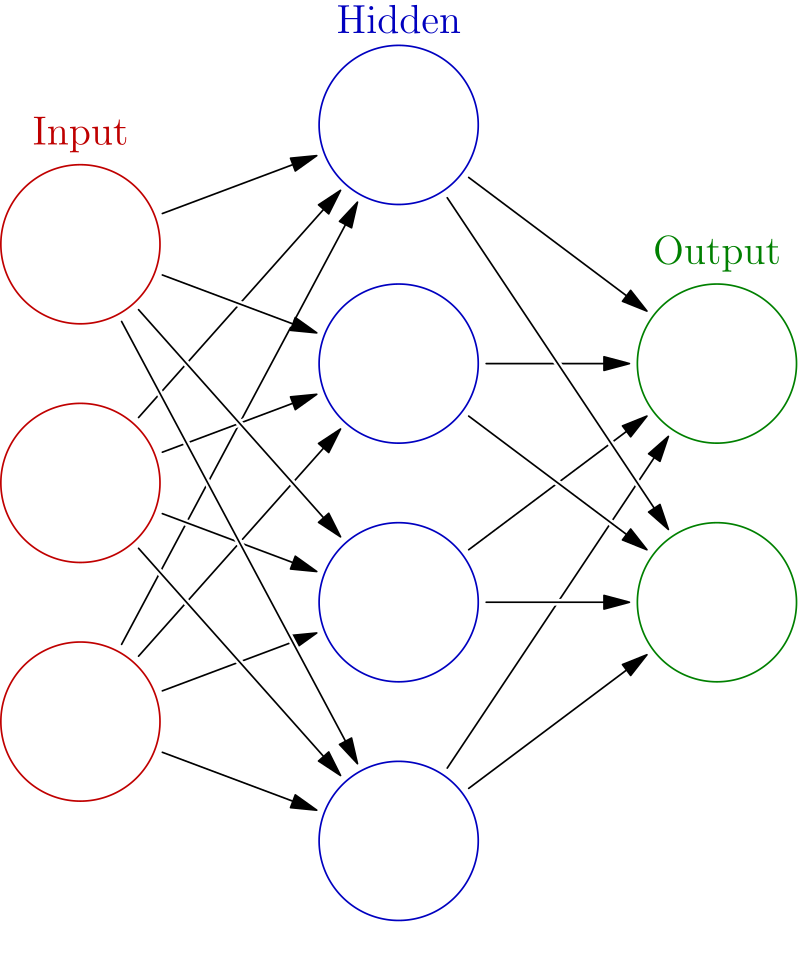
\includegraphics[width=0.17\textwidth, align=c]{Ch1_Intro/Colored_neural_network.png} \\
        (e) Predicting links in social networks~\citep{zhou2020graph} & (f) Predicting properties of neural networks\textsuperscript{1} \\
        
    \end{tabular}
    \caption{\small Example applications of graph reasoning methods. \textsuperscript{1}Images are obtained from {\footnotesize \url{https://en.wikipedia.org/wiki/Artificial_neural_network}} and {\footnotesize \url{https://en.wikipedia.org/wiki/Biological_neuron_model}}.}
    \label{fig:intro_apps}
    %\vspace{-10pt}
\end{figure}




To develop algorithms able of inferring a compositional structure from raw sensory data or algorithms predicting structure's properties, we first need to define a data abstraction suitable for this kind of tasks.
In mathematics and computer science there exists a convenient abstraction specifically introduced to model compositional and relational structures. This abstraction is called a graph, in which nodes correspond to the components of the structure and edges correspond to interactions between the components.
For example, molecules are often represented as graphs with nodes corresponding to atoms or more complex elements and edges corresponding to chemical bonds (Fig.~\ref{fig:intro_apps}, d). Similarly, social networks are graphs with nodes being people and edges being different kinds of relationships between them (Fig.~\ref{fig:intro_apps}, e). Likewise, a biological or artificial neural network is a graph wherein nodes can be neurons and edges can be connections between them (Fig.~\ref{fig:intro_apps}, f). 
Having modeled data as graphs, algorithms tackling the associated tasks need to be developed.


Tasks illustrated in \fig{\ref{fig:intro_apps}} can be approached by manually designing task-specific rules or algorithms. However, recently there has been a spike in performance on such tasks using deep learning methods. In particular, deep neural networks (DNNs) require less human interventions and instead learn task-specific rules and algorithms from data and experience. DNNs currently dominate across visual, language and graph tasks~\citep{lecun2015deep}. Specifically, state-of-the-art convolutional neural networks (CNNs)~\citep{krizhevsky2012imagenet,he2016deep} reach or even outperform~\citep{he2015delving,cai2019onceforall} humans in tasks such as large-scale image classification, \eg ImageNet~\citep{russakovsky2015imagenet}. In the graph domain, many tasks have been successfully solved by DNNs operating on graphs, called Graph Neural Networks (\gnns)~\citep{gori2005new, scarselli2008graph, bronstein2017geometric,zhou2020graph}. 
DNNs continue to improve and extend their scope, becoming an essential part of real world applications~\citep{brown2020language}.

\begin{figure}[tbhp]
    \centering
    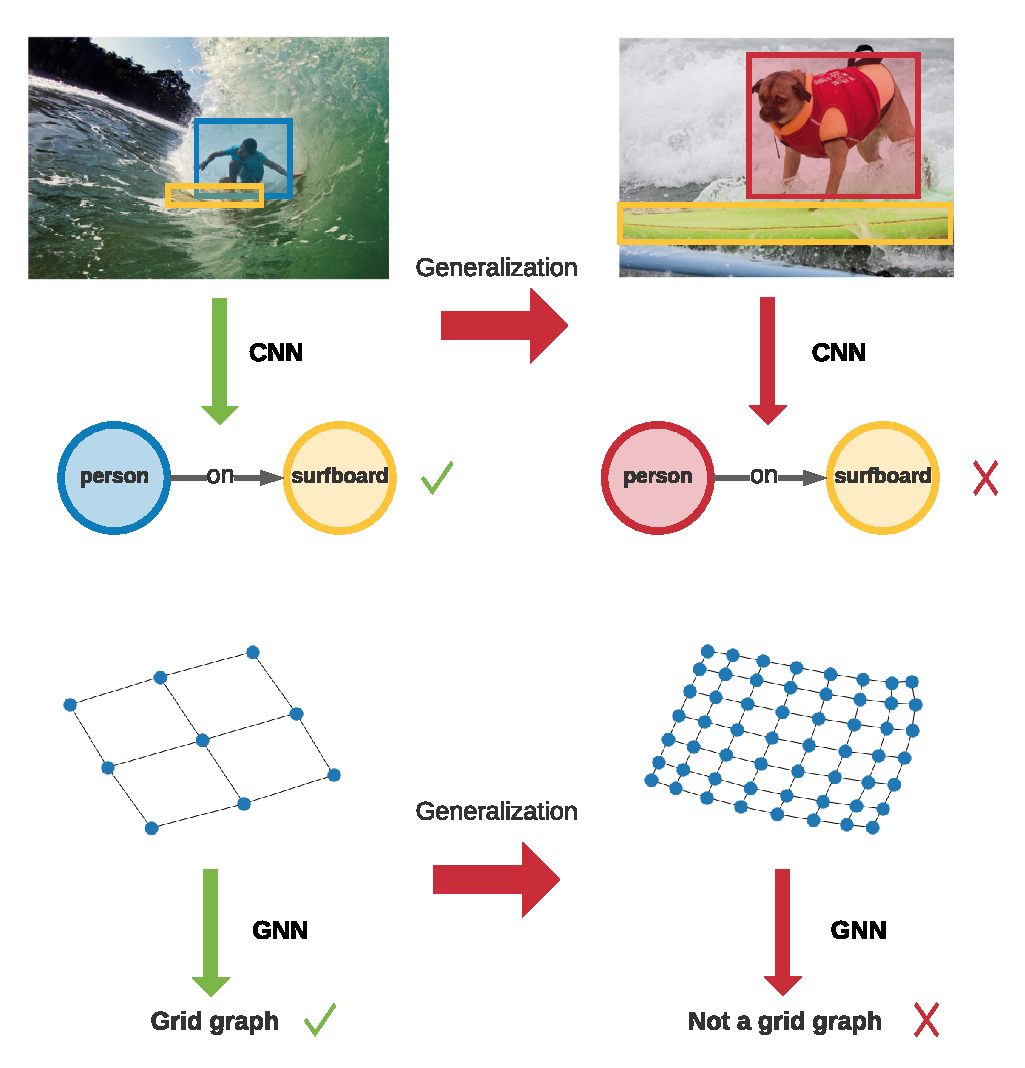
\includegraphics[width=0.6\textwidth, align=c]{Ch1_Intro/intro_generalization.pdf}
    \vspace{-10pt}
    \caption{\small Machine learning methods for images, graphs and other domains can accurately reason about the \IID samples (left). However, reasoning on test samples that are somewhat different from or correspond to the tail of the training distribution (right) remains challenging. In the graph example (bottom), both the small and large graph represent so called grid (mesh or lattice) graphs. }
    \label{fig:intro_generalization}
\end{figure}

Despite the extreme success of DNNs, they have certain limitations and this thesis mainly addresses the two of them. The first challenge is fundamental and concerns the decrease of DNNs' performance when they observe somewhat unusual inputs~\citep{hendrycks2019benchmarking,galloway2019batch,szegedy2013intriguing}. For example in the image domain, the dog on a surfboard can be confused with a person, since in the data used to train CNNs persons appear more frequently on surfboards than dogs (\fig{\ref{fig:intro_generalization}}, top). In the graph domain, a GNN trained to reason about smaller graphs, can fail to accurately reason about larger graphs~\citep{yehudai2021local} (\fig{\ref{fig:intro_generalization}}, bottom).
While there is still limited understanding what exactly makes CNNs or GNNs fail in such cases, a high-level explanation is that learning-based methods make an assumption that all training and test samples are independently and identically distributed (\IID)~\citep{shen2021towards}. In practice (as illustrated in \fig{\ref{fig:intro_generalization}}), this assumption is often violated, leading to inaccurate predictions or poor generalization. 
%In machine learning terms, such DNNs are not robust or do not generalize well to distribution shifts. 
Such behavior is often unacceptable in critical applications such as self-driving cars or health care, where errors can be fatal.
To highlight this issue and develop a more rigorous understanding of DNNs' generalization properties, a variety of research frameworks have been proposed~\citep{lust2020survey,shen2021towards,hendrycks2019benchmarking,hupkes2019compositionality,garg2020generalization}. Despite these efforts, in many tasks the progress remains slow. For instance, in the scene graph generation task state-of-the-art CNNs show a $\sim$10 fold decrease in performance on test images containing unusual or unseen visual compositions~\citep{tang2020unbiased,knyazev2020graph,suhail2021energy}. In this thesis, we develop empirical frameworks to study generalization failure in CNNs and GNNs, leading to improvements in the visual and graph domains respectively.\looseness-1

The second limitation of DNNs pertains to the challenge of extending their scope to more problems where manually-designed algorithms still dominate. Before the rise of DNNs, researchers and practitioners focused tremendous efforts on designing features to better solve a concrete task, \eg image classification~\citep{lowe2004distinctive}. The advent of deep learning showed that in many settings features learned by DNNs outperformed features designed by humans~\citep{krizhevsky2012imagenet}. This encouraged researchers and practitioners to extend the scope of DNNs in many directions. One notable direction has been the design of stronger DNN architectures\footnote{Generally speaking, a DNN architecture is defined by the types of neural network layers, their number and connectivity between them.} to better solve a given task. Similar to pre-deep learning feature design, architecture design has been recently overtaken by neural architecture search methods that \emph{learn} a DNN architecture, replacing and outperforming human-designed DNN architectures~\citep{zoph2016neural,liu2018darts,ren2020comprehensive}.
Yet many aspects of DNN practice still require much human engineering effort. 


In particular, optimization algorithms used to train DNNs are still manually-designed.
For example, one of the dominant algorithms is stochastic gradient descent (SGD). SGD is a manually-designed algorithm based on computing gradients \wrt a highly \textit{non-convex} loss function and the gradient-based rules to update DNN parameters according to \textit{convex} optimization theory~\citep{jain2017non}. Replacing optimization algorithms such as SGD with DNN counterparts may reveal more optimal update rules~\citep{andrychowicz2016learning}. Learnable optimizers remain one of the oldest directions that still have only limited success~\citep{schmidhubermetalearning,metz2020tasks}.
Yet, by analogy with other successful directions, if DNNs could replace SGD, then dramatic advances might follow. In this thesis, we make a step towards that long-standing and ambitious goal. Specifically, we develop graph reasoning methods that allow us to predict performant parameters of DNNs represented as graphs. Following the focus of previous chapters on aspects of generalization, we take into consideration samples beyond \IID when developing and evaluating parameter prediction methods. This extends the scope of this thesis to more practical and challenging scenarios.\looseness-1

\graphicspath{{Ch2_background/}}

\chapter{Background\label{sec:bg}}

We consider prediction problems where we are given inputs and need to make some decision about them. In the context of image recognition, let us consider images of natural objects (\eg dogs) as input. The task is to predict semantic content in the image. We will consider the image classification task where a single label per image (\eg `dog' or `person') must be predicted, and more complex tasks where rich description (\eg `dog on surfboard') must be predicted (\fig{\ref{fig:problem}}).%\looseness-1

\begin{figure}[htbp]
    \centering
     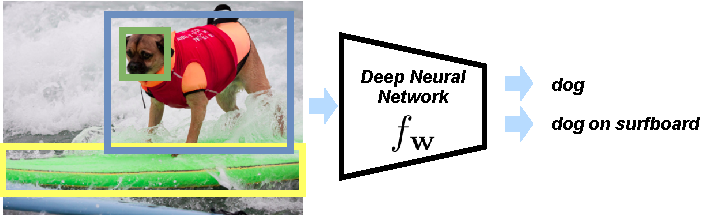
\includegraphics[width=0.9\textwidth, align=c]{figs/problem_form.pdf} 
    \caption{Prediction of object categories and their relationships given an image.}
    \label{fig:problem}
\end{figure}


\section{Neural networks\label{sec:bg_nn}}
In image recognition tasks,
%, such as image classification, 
the input is high dimensional\footnote{Image resolution varies drastically between image tasks, but generally represent high-dimensional cases. For example, in MNIST~\citep{lecun1998gradient}, the images are 28$\times$28 pixels, \ie 784 dimensional. In more realistic tasks, such as PASCAL~\citep{everingham2010pascal}, images can be 500$\times$300 pixels, \ie 150,000 dimensional.} and the decision process is hard to formally describe using simple expert rules and raw inputs.
Therefore, the currently dominant strategy to solve such a task is to formulate it as an optimization problem:
%
\begin{equation}
    \w^* = \underset{\w}{\text{arg\,min }} \ \mathcal{L}(f_\w, \mathcal{D}),
\end{equation} 
%
%$\in \mathcal{D}$
\noindent where $f_\w$ is some function parameterized by $\w$, $\mathcal{D}$ is the dataset associated with the task and $\mathcal{L}$ is the objective to minimize for this dataset. The goal of solving this problem is to find optimal parameters $\w^*$ for $f_\w$.
For large and complex datasets, the state-of-the-art solutions to this optimization problem are often based on using deep neural networks (DNNs) as $f_\w$. Finding globally optimal $\w^*$ of DNNs is generally intractable due to the highly non-convex nature of $\mathcal{L}(f_\w, \mathcal{D})$~\citep{choromanska2015loss}. Nevertheless, local optima can be found using methods based on gradient descent~\citep{ruder2016overview,kingma2014adam}.\looseness-1

%The design of DNNs varies drastically depending on the task. 
DNNs can have drastically different designs depending on the task. This thesis concerns three different designs of DNNs. The first is one of the earliest types of DNNs, colloquially referred to as a multilayer perceptron (MLP). Next, we consider convolutional neural networks (\cnns) -- DNNs designed specifically for perceptual tasks, such as image recognition. Lastly, we consider graph neural networks (\gnns) that are designed for graph-structured data. MLPs, \cnns and \gnns are the core building blocks of this thesis.
%\footnote{Some portions of \S~\ref{sec:bg_nn} are based on my blog posts: \url{https://medium.com/@BorisAKnyazev}}.

\subsection{Multilayer perceptrons\label{sec:bg_mlp}}
MLPs or, more precisely, multilayer feedforward fully-connected neural networks, consist of $L$ layers of trainable parameters (weights) $\w = [\W^{(1)}, \W^{(2)}, ..., \W^{(L)}]$. Given $N$ input data points $\X \in \R^{N \times d} $ of dimensionality $d$ from the dataset $\mathcal{D}$, the MLP sequentially transforms the input $\X$ as\footnote{For simplicity, in \eqref{eq:mlp} we ignore the bias term $\mathbf{b}$ that in practice is added to the output of $\X^{(l)}\W^{(l)}$. The bias is essential when a single layer is used, however it has limited practical value in the case of $L > 1$.}:
%
\begin{equation}
    \label{eq:mlp}
    \X^{(l+1)} = \sigma(\X^{(l)}\W^{(l)}),
\end{equation}
%
\noindent where $l \in [1,L]$ and an input to the first layer $\X^{(1)}$ is equal to $\X$. Function $\sigma$ is some nonlinearity such as the Rectified Linear Unit (ReLU) applied element-wise to $\X^{(l)}\W^{(l)}$: $\sigma (\X^{(l)}\W^{(l)})=\max(0, \X^{(l)}\W^{(l)})$. More advanced nonlinearities can lead to better training and generalization properties, e.g. leaky ReLU~\citep{maas2013rectifier} or the Exponential Linear Unit (ELU)~\citep{clevert2015fast}. Applying $\sigma$ is essential to learn nonlinear transformations. One of the simplest nonlinear transformations is the XOR logic operation that was famous in diminishing the interest in AI (``AI winter'') in the 1970s\footnote{More about that period can be read at \url{https://dev.to/jbahire/demystifying-the-xor-problem-1blk} or \url{https://towardsdatascience.com/history-of-the-first-ai-winter-6f8c2186f80b}.}. For the final layer ($l=L$), it is common to use a nonlinearity specific for the task. For example, in the case of predicting binary labels $\mathbf{y} \in [0,1]^N$ for data points $\X$, a sigmoid function can be applied. In the case of regression tasks, $\mathbf{y} \in \R^N$, \ie, the final nonlinearity is removed.
All $N$ data points in $\X$ can be processed by MLPs independently, so parallel computing enables very efficient usage of MLPs. $N$ data points processed in parallel are often called a mini-batch, or batch\footnote{When ``batch'' and ``mini-batch'' are used to describe the operation of learning, batch means updates based on the entire dataset and mini-batch means updates based on a subset.}.\looseness-1
%Multiple layers with interleaved nonlinearities are required to learn such and more complex transformations.
%For example an MLP with a single layer of parameters $\W \in \R^{d_1 \times d_2}$: $f(\X, \W) = \X\W$. 
%The MLP layers can be stacked to form a deep network: $f(\X, \W) = (\sigma(\X\W^{1}))\W^{2}$, where $\sigma$ is some nonlinearity such as ReLU to learn a nonlinear transformations. 
%Without $\sigma$ multiple layers will be equivalent to a single layer thus preventing learning complex transformations.
\paragraph{Applications of MLPs.} MLPs can be in principle applied to any tabular data $\X$ where rows are data points and columns are features or dimensions. While images can be represented as tabular data by flattening spatial dimensions~\citep{ciregan2012multi}, MLPs are more common in cases when the dimensions in $\X$ are not ordered in any meaningful way (\ie there is no benefit of leveraging the order).
%(\ie the order can be changed without affecting the training procedure).
MLPs are often used as building blocks of many other types of DNNs, including recently developed Transformers~\citep{vaswani2017attention,dosovitskiy2020image} and Graph Neural Networks~\citep{kipf2016semi} (\S~\ref{sec:bg_gnn}). Oftentimes, the last few layers of Convolutional Neural Networks (\S~\ref{sec:bg_cnn}) are modeled as MLPs~\citep{simonyan2014very}.
Recently, models based on MLPs were revisited in large-scale image tasks, where they showed competitive results~\citep{touvron2021resmlp}.\looseness-1

\subsection{Convolutional neural networks\label{sec:bg_cnn}}

The main building blocks of \cnns, convolution and downsampling, were introduced in~\citep{fukushima1982neocognitron}.
%Convolution and downsampling are the main building blocks of CNNs~\citep{fukushima1982neocognitron}. 
Subsequently, in \citep{lecun1998gradient}, \cnns were combined with a gradient descent-based training algorithm to effectively learn the parameters of \cnns from raw inputs (images) without manually engineering features.
Following~\eqref{eq:mlp} for the MLP layer, the convolutional layer for $N$ images ${\cal X} \in \R^{N \times C \times H \times W}$ and $K$ filters (kernels, weights) $\mathcal{W} \in \R^{K \times C \times h \times w}$ can be defined as~\citep{vedaldi2015matconvnet}:
%
\begin{equation}
    \label{eq:conv}
    {\cal X}_{n,k,i,j}^{(l+1)} = \sigma(\sum_c \sum_h \sum_w {\cal X}_{n,c,i-h,j-w}^{(l)} {\cal W}_{k,c,h,w}^{(l)}),
\end{equation}
%
\noindent where $C$ is the number of channels (\eg $C=3$ for RGB images); $H,W$ are the height and width of images respectively; $K$ is the number of filters and $h,w$ are their height and width respectively. Each $k$-th filter of $\mathcal{W}$ slides over the input along the spatial dimensions and for each spatial location $i \in [1,H], j \in [1,W]$ of $\mathcal{X}$ computes the dot product between the local region and the kernel (\fig{\ref{fig:conv}}).\looseness-1


\begin{figure}[htbp]
    \centering
    \footnotesize
    \begin{tabular}{cccc}
    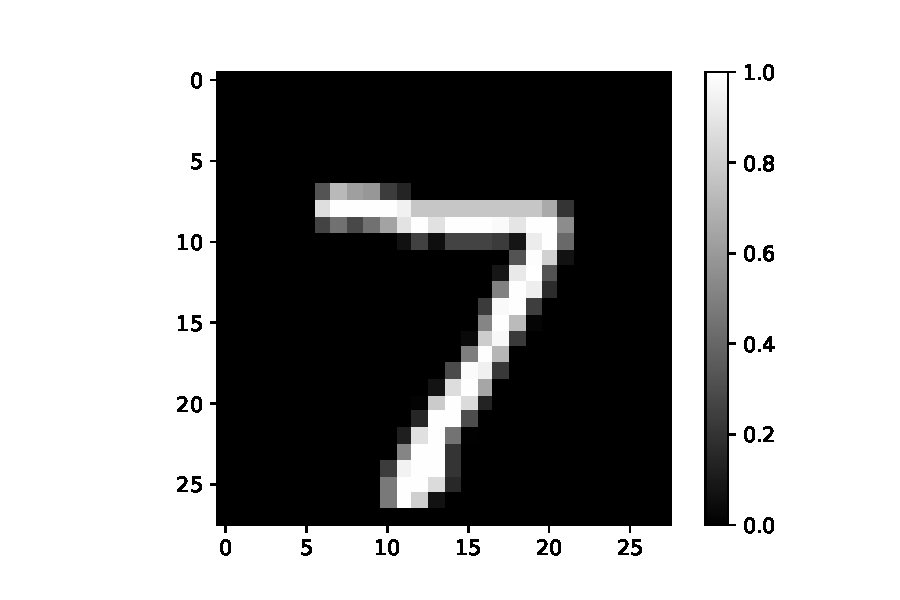
\includegraphics[width=0.22\textwidth]{figs/mnist_digit.pdf} & 
    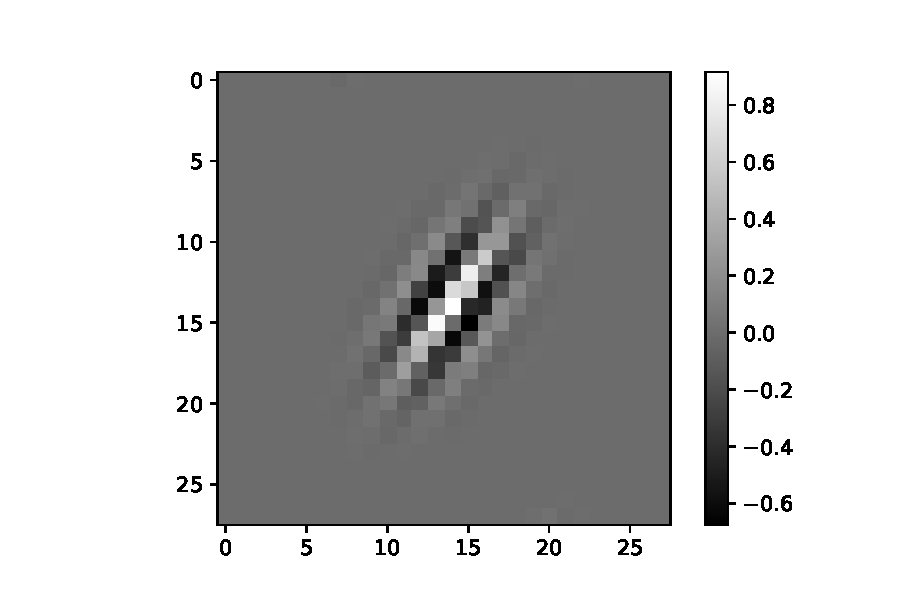
\includegraphics[width=0.22\textwidth]{figs/conv_kernel.pdf} & 
    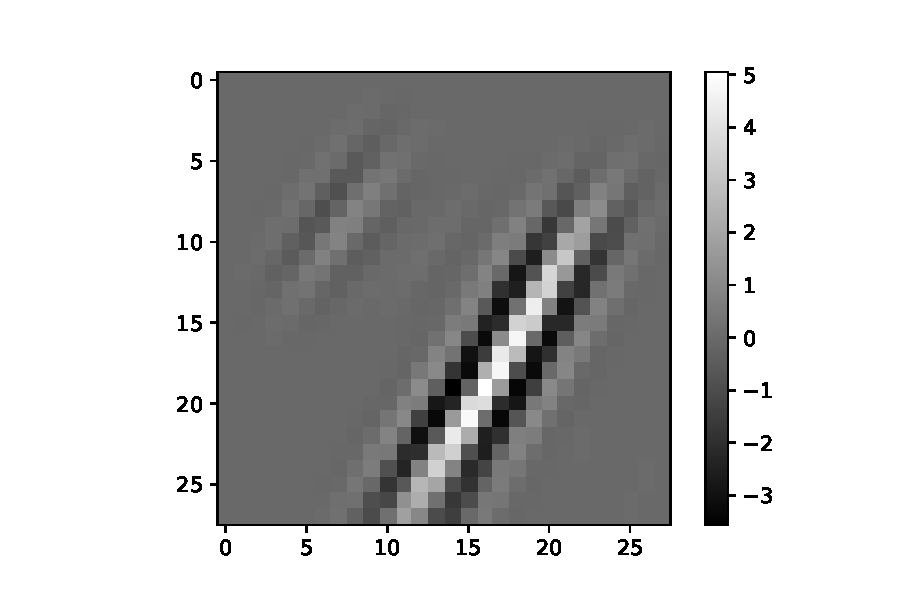
\includegraphics[width=0.22\textwidth]{figs/conv_output.pdf} & 
    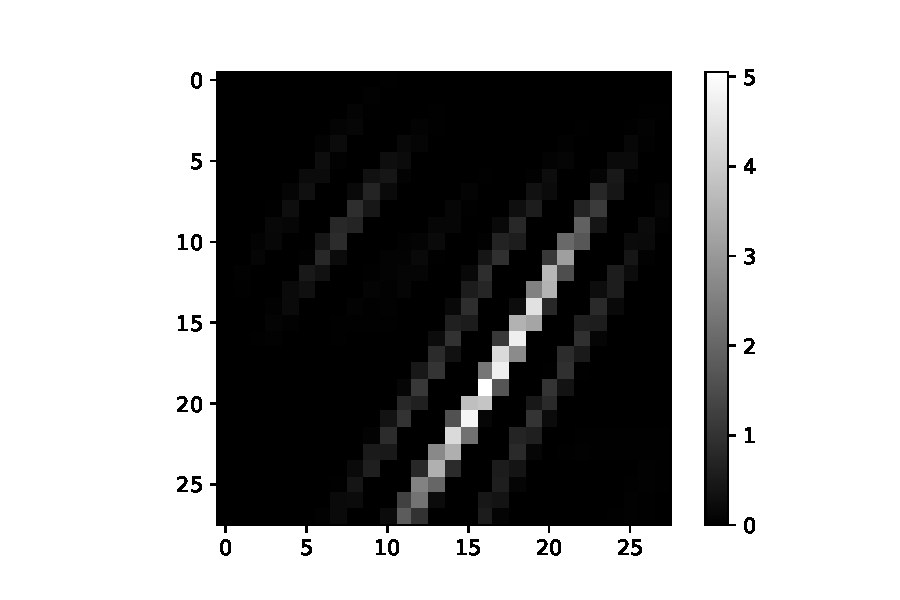
\includegraphics[width=0.22\textwidth]{figs/relu_output.pdf} \\
    Input image & Convolutional filter & Output of convolution & Output after ReLU \\
    \end{tabular}
    \caption{Example of the convolution operation for a single image and single filter.}
    \label{fig:conv}
\end{figure}

The convolution operation exploits a 2D local structure in images, formally described in~\citep{bronstein2017geometric}:
\vspace{-3pt}
\begin{itemize}
    \setlength{\itemsep}{1pt}
    \item Shift-invariance -- if we spatially translate an object on the image to the left/right/up/down, we still should be able to recognize it. This is exploited by sharing filters across all locations.
    \item Locality -- nearby pixels are closely related and often represent some semantic concepts, such as object parts. This is exploited by using filters with spatial dimensions $h > 1$ and $w > 1$, which can capture image features in a local spatial neighborhood.
    \item Compositionality (or hierarchy) -- a larger region in the image is often a semantic parent of smaller regions it contains. For example, a dog is a parent of a head, body, legs, etc. 
    %Likewise, the head is a parent of ears, nose, eyes, etc. 
    This implicitly is exploited by stacking convolutional layers.
\end{itemize}

Another important component of \cnns is the downsampling operation. Downsampling reduces the spatial size of inputs, which is important for computational efficiency, particularly for large inputs. Downsampling is usually based on spatial pooling applied to a local region similar to convolution. Typically, average or max poolings are used that do not have trainable parameters. In practice, pooling can be replaced with modified (strided) convolution to simplify the overall network~\citep{springenberg2014striving}.\looseness-1

As compared to MLPs, \cnns applied to images have another strength besides those listed above. In particular, the number of trainable parameters in convolutional filters $\mathcal{W}$ does not depend on the input spatial dimensions $H,W$. In principle, the same \cnn can be trained on images with $H=W=28$ as well as $H=W=500$. In addition, \cnns are highly efficient due to their ability to apply filters $\mathcal{W}$ independently and in parallel for each spatial location, each filter and each image. As a result, \cnns have been adapted to a broad range of tasks beyond image classification.
%In other words, the model is parametric.

\vspace{-3pt}
\paragraph{Applications of \cnns.} \cnns initially were proposed for simple image classification tasks, such as handwritten digit recognition (MNIST)~\citep{lecun1998gradient}. Subsequently, a larger and deeper network proposed in \citep{krizhevsky2012imagenet} led to the top-1 result on the ImageNet 2012 challenge of large-scale image classification~\citep{russakovsky2015imagenet} outperforming hand-designed visual features such as SIFT~\citep{lowe2004distinctive}.
Compared to~\citep{lecun1998gradient}, the main changes made in \citep{krizhevsky2012imagenet} to \cnns were: i) dramatically increased size of a \cnn possible due to larger and cheaper computational resources available, ii) a large annotated dataset (\ie ImageNet), iii) applying nonlinearities and regularization methods such as ReLU and Dropout~\citep{hinton2012improving}.
Since then, \cnns have dominated visual tasks~\citep{gu2018recent} and grown significantly in size showing superior results in image and video object
%(\eg a dog, a surfboard in \fig{\ref{fig:problem}})
detection~\citep{ren2015faster,wang2017video,he2016deep,he2015delving}, image and video semantic segmentation~\citep{long2015fully,shelhamer2016clockwork}, video recognition~\citep{simonyan2014two}, image and video generation~\citep{goodfellow2014generative,vondrick2016generating}, learning to estimate the optical flow between a pair of images~\citep{dosovitskiy2015flownet}, and many other tasks.
In these and more complex tasks, such as visual question answering (VQA)~\citep{antol2015vqa}, \cnns are typically used as a ``backbone'' to extract visual features from images. The same backbone and its trained parameters can be used across different tasks. The procedure of reusing the backbone parameters from one task to improve on another task is called ``transfer learning''. Typically, backbones trained on large image tasks such as ImageNet show the best transfer learning abilities~\citep{huh2016makes,kornblith2019better}.
%``Transfer learning'' is a common practice in/for X that transfer \cnns pretrained on large image datasets such as ImageNet. 
Finally, \cnns' computational efficiency has been significantly improved. In particular, architectural enhancements~\citep{howard2017mobilenets,cai2019onceforall}, as well as compression and distillation techniques~\citep{cheng2017survey} together with very efficient implementations~\citep{chetlur2014cudnn} enabled the deployment of \cnns on low-resource mobile devices further extending \cnns' application reach.\looseness-1
% to a downstream task
%For example, object detectors predict a set of bounding boxes (x,y,width,height) for each object and their category. In \fig{\ref{fig:problem}} the object detector should detect a dog, surfboard, wave and, ideally, fine-grained details such as vest and dog's body parts.
%The widespread utility of \cnns is reinforced by their efficiency, which is due to the parallelization of the convolution operation. \looseness-1

%\cnns are the main backbone of computer vision models, such as object detectors~\citep{ren2015faster}. 

\subsection{Graph neural networks\label{sec:bg_gnn}}

The wide success of \cnns have motivated their application to more tasks.
%methods in other tasks where 
%One of such tasks is learning from graph-structured data. 
In tasks such as chemistry, physics and social networks,
% Graph-structured data are ubiquitous in
%, transportation, 3D geometry, visual reasoning, and others
the data are represented as graphs. 
%However, applying \cnns to graphs is not straightforward as there is no notion of spatial translation in graphs. 
However, convolution \eqref{eq:conv} requires data to reside on a ``regular grid'', a Euclidean coordinate system where all the data points are located at the discrete and equally spaced coordinates consistent among all samples~\citep{bronstein2017geometric}. For example, all MNIST images reside on the same 28$\times$28 regular grid. In contrast, graphs generally reside on ``irregular grids'' that do not have a notion of spatial translation, preventing the application of convolution as per \eqref{eq:conv}.\looseness-1

Formally, a graph $\G$ consists of an unordered set of $N$ nodes, $\V$, connected by edges, $\E$. 
The edges are often encoded by an adjacency matrix $\A \in \R^{N \times N}$. The number of neighbors for each node can be then defined as a diagonal matrix $\D$, where $\D_{ii} = \sum_j \A_{ij}$. %, which is binary if the graph is unweighted.
Defining convolution on graphs is non-trivial because the nodes are generally unordered, and not attached to a particular coordinate system, and the node degree $\D_{ii}$ can vary for each $i$-th node.

To define convolution on graphs, a spectral graph theory has been applied~\citep{bruna2013spectral}. This theory is based on extending the spectral definition of convolution in signal processing. For signals, we can define spectral convolution equivalent to the spatial definition in~\eqref{eq:conv} using the Discrete Fourier Transform. Similarly, spectral convolution on graphs can be computed~\citep{belkin2001laplacian,chung1997spectral,bruna2013spectral}\footnote{An extended description of defining spectral convolution on graphs can be found in my blog post: \url{https://towardsdatascience.com/spectral-graph-convolution-explained-and-implemented-step-by-step-2e495b57f801}.} based on the eigendecomposition of the graph Laplacian $\Lapl = \mathbf{I}_N - \D^{-1/2}\A\D^{-1/2}$, where $\mathbf{I}_N$ is an $N \times N$ identity matrix. In particular, the eigendecomposition of $\Lapl$ is defined as $\Lapl=\mathbf{V}\mathbf{\Lambda}\mathbf{V}^T$, where $\mathbf{V}$ are eigenvectors and $\mathbf{\Lambda}$ are eigenvalues.
Given node features $\X^{(l)} \in \R^{N \times d}$, the spectral graph convolution layer with filters $\W^{(l)}$ can be then defined as:
%
\begin{equation}
 \label{eq:graph_spectral_conv}    
 \X^{(l+1)} = \sigma \Big( \mathbf{V} (\mathbf{V}^T\X^{(l)} \odot \mathbf{V}^T\W^{(l)}) \Big),
\end{equation}
%
\noindent where $\odot$ is element-wise multiplication. Similarly to the spectral convolution in signal processing, in \eqref{eq:graph_spectral_conv} the features and filters are first projected into the spectral domain where they are multiplied. The result is then reconstructed back to the original domain.

A major disadvantage of spectral graph convolution defined in \eqref{eq:graph_spectral_conv} is the necessity to compute the eigendecomposition for each graph. In many graph tasks, graphs have very different structures (and different eigenvectors $\mathbf{V}$) and it is unclear if the same $\W^{(l)}$ can adapt to different $\mathbf{V}$~\citep{nilsson2020experimental}. 
%For example, at test time, for a new graph and a new set of eigenvectors, these filters might be inappropriate.
Moreover, computing eigendecomposition for large graphs is a computationally intensive process.
To eliminate the need of eigendecomposition, %\citet{defferrard2016convolutional} proposed to approximate \eqref{eq:graph_spectral_conv} with Chebyshev polynomials of order $K \in [1, N]$. Chebyshev convolution aggregates node features within the $K$-hop neighborhood. 
spectral graph convolution \eqref{eq:graph_spectral_conv} can be approximated using recursive Chebyshev polynomials $T_k$ and the property of eigendecomposition that $\Lapl^k=(\mathbf{V} \mathbf{\Lambda} \mathbf{V}^T)^k = \mathbf{V} \mathbf{\Lambda}^k \mathbf{V}^T$.
To derive approximate Chebyshev graph convolution, 
the polynomials $T_k$ are first applied to the rescaled graph Laplacian $\tilde{\Lapl}=2\Lapl/\lambda_{\max} - \mathbf{I}_N$~\citep{hammond2011wavelets, defferrard2016convolutional}:\looseness-1
%
\begin{equation}
\label{eq:cheb_lapl}
T_k(\tilde{\Lapl}) = 2 \tilde{\Lapl} T_{k-1}(\tilde{\Lapl}) - T_{k-2}(\tilde{\Lapl}), 
\end{equation}
%
\noindent where $k \in [1, N]$, $T_0(\tilde{\Lapl}) = \mathbf{I}_N$ and $T_1(\tilde{\Lapl}) = \tilde{\Lapl}$; $\lambda_{\max}$ is the largest eigenvalue of $\Lapl$.
Using \eqref{eq:cheb_lapl} and the aforementioned property of eigendecomposition that $\Lapl^k= \mathbf{V} \mathbf{\Lambda}^k \mathbf{V}^T$, \citet{hammond2011wavelets, defferrard2016convolutional} derived that spectral graph convolution can be approximated as a sum of the $T_k(\tilde{\Lapl})$ terms weighted by trainable parameters $\W^{(l)}_k$. Hence, the Chebyshev graph convolution layer can be defined as:
%
\begin{equation}
\label{eq:cheb_graph_conv}
\X^{(l+1)} = \sigma \Big(\sum^{K-1}_{k=0} T_k(\tilde{\Lapl}) \X^{(l)} \W^{(l)}_k \Big),
\end{equation}
%
\noindent where $K \in [1, N]$ is a hyperparameter controlling how global is the receptive field of the convolution. In particular, the terms $T_k(\tilde{\Lapl})$ include powers $\tilde{\Lapl}^k$ enabling a $(k-1)$-hop receptive field and allowing to approximate spectral convolution. For example, for $K=N$ the convolution \eqref{eq:cheb_graph_conv} is performed globally based on the entire graph structure making it approximately equal to spectral convolution \eqref{eq:graph_spectral_conv}. For $K=1$ we have $T_0(\tilde{\Lapl}) = \mathbf{I}_N$, so the convolution is performed ignoring the graph structure, while for $K=2$ the convolution is performed based on the 1-hop neighborhood of nodes, and so forth.
Stacking Chebyshev graph convolution layers \eqref{eq:cheb_graph_conv} form a graph neural network called a ChebyNet studied in our works~\citep{knyazev2018spectral,knyazev2019image,knyazev2019understanding}.

\citet{kipf2016semi} studied the 1-hop Chebyshev graph convolution (with $K=2$) and proposed its highly-effective and efficient simplification:\looseness-1
%
\begin{equation}
    \label{eq:graph_conv_kipf}
    \X^{(l+1)} = \sigma(\hat{\A}\X^{(l)}\W^{(l)}),
\end{equation}
%
\noindent where $\hat{\A}$ is a normalized adjacency matrix similar to the rescaled graph Laplacian $\tilde{\Lapl}$: $\hat{\A} = \tilde{\D}^{-1/2}\tilde{\A}\tilde{\D}^{-1/2}$, and $\tilde{\D}_{ii} = \sum_j \tilde{\A}_{ij}$; $\tilde{\A} = \A + I_N$ to include self-loops into convolution. Essentially, \eqref{eq:graph_conv_kipf} combines the first two terms of \eqref{eq:cheb_graph_conv} for $k=[1,2]$ into a single operation. The model based on multiple convolutions \eqref{eq:graph_conv_kipf} is commonly referred to as a graph convolutional network (GCN). In this thesis, we will use a more general term ``graph neural network'' (\gnn) to refer to this and other graph models.\looseness-1

The graph layer defined in~\eqref{eq:graph_conv_kipf} is remarkably similar to the one of the MLP layer~\eqref{eq:mlp}. The only difference is the normalized adjacency matrix $\hat{A}$ used in~\eqref{eq:graph_conv_kipf}. Therefore, a \gnn can be viewed as an MLP exploiting the relational information between data points (or node features). 

Following the example in \fig{\ref{fig:conv}} (\S~\ref{sec:bg_cnn}), graph convolution \eqref{eq:graph_conv_kipf} can be illustrated based on an MNIST image. To represent an image as a graph, nodes correspond to pixel coordinates and edges connect only four spatially adjacent pixels (\fig{\ref{fig:graph_conv}}). In the graphs, pixel intensities are inverted for better visualization with black nodes corresponding to white pixels. The image is resized to 14$\times$14 and a small amount of Gaussian noise is added to illustrate the effect of graph convolution. To compute the output, only $\hat{\A}\X^{(l)}$ is used while $\W^{(l)}$ is ignored. Such graph convolution is equivalent to a low-pass mean filter commonly used in signal processing to denoise the signal. The low-pass effect helps \gnns to excel in tasks where aggregating 1-hop node features is sufficient for high performance. However, 1-hop low-pass filtering also limits the expressive power of \gnns in tasks where complex long-range interactions between nodes are important~\citep{nt2019revisiting,knyazev2019image}.~\looseness-1


\begin{figure}[htbp]
    \centering
    \newcommand{\figwidth}{0.16\textwidth}
    \begin{tabular}{ccc}
        {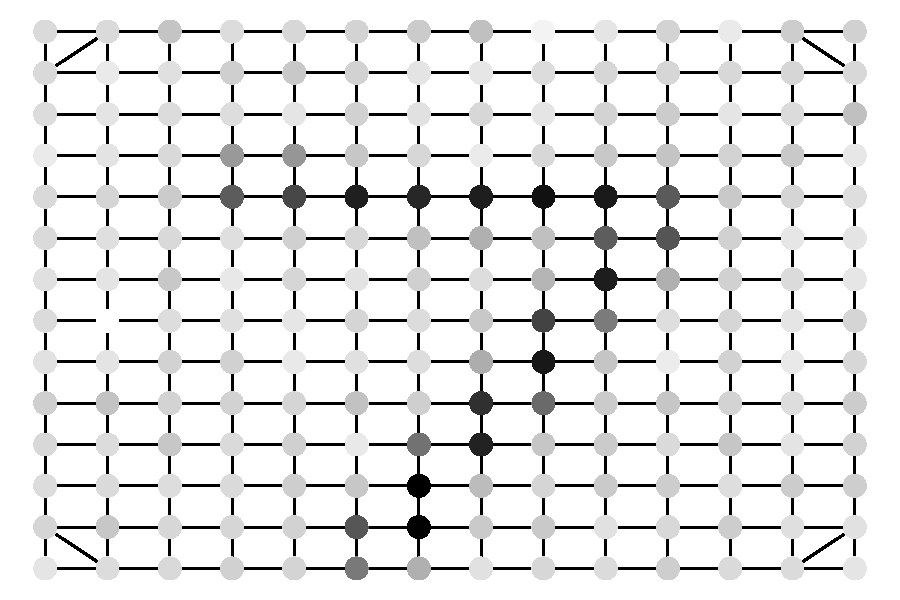
\includegraphics[width=\figwidth,height=\figwidth,clip,trim={1.65cm 0 1.65cm 0}]{figs/graph_conv_in.pdf}} &  
        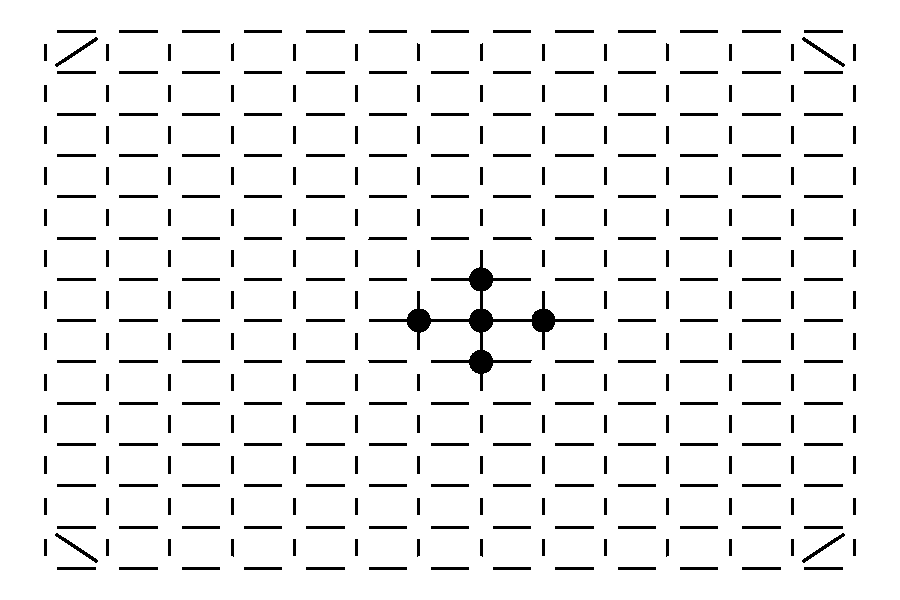
\includegraphics[width=\figwidth,height=\figwidth,clip,trim={1.65cm 0 1.65cm 0}]{figs/graph_conv_kernel.pdf} &
        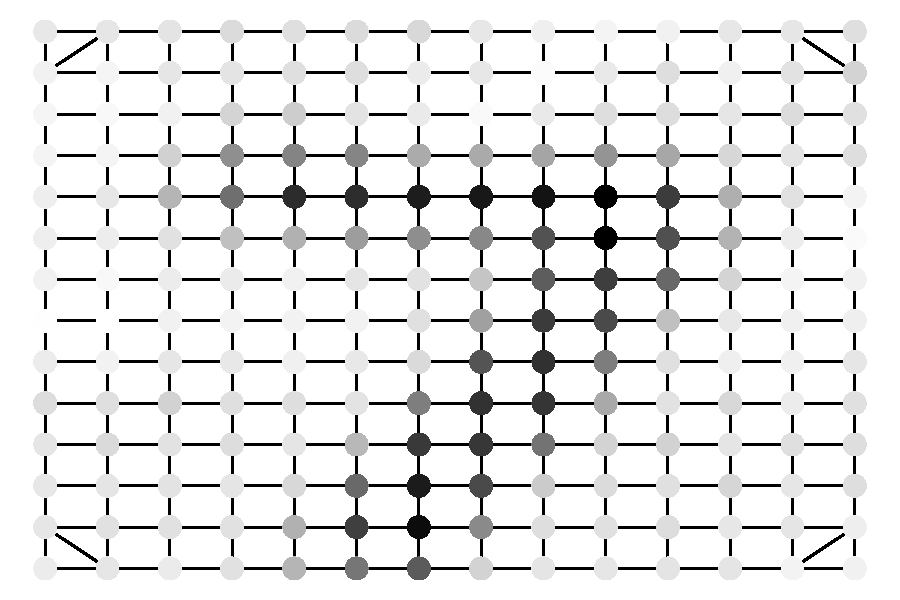
\includegraphics[width=\figwidth,height=\figwidth,clip,trim={1.65cm 0 1.65cm 0}]{figs/graph_conv_out.pdf} \\
        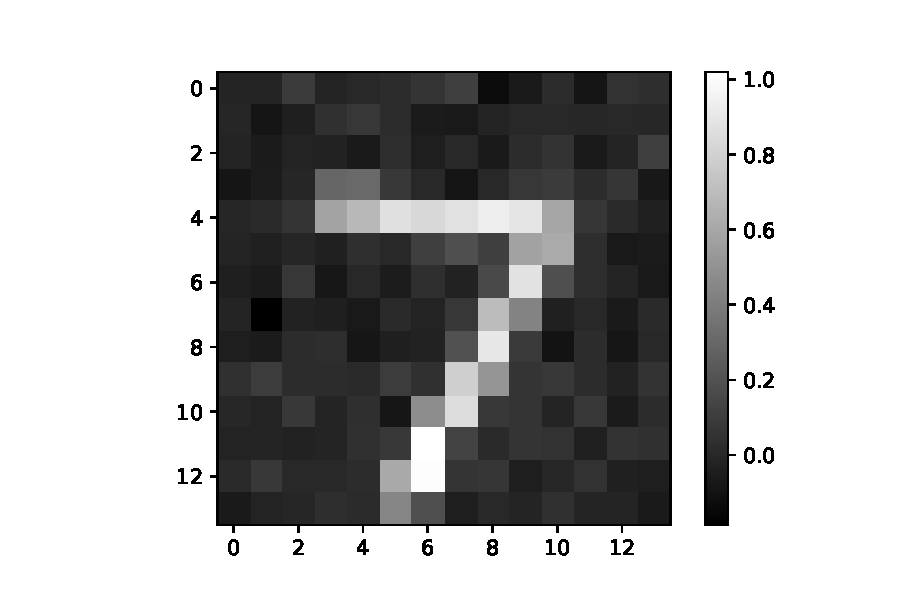
\includegraphics[width=0.27\textwidth]{figs/graph_conv_in_im.pdf} &  
        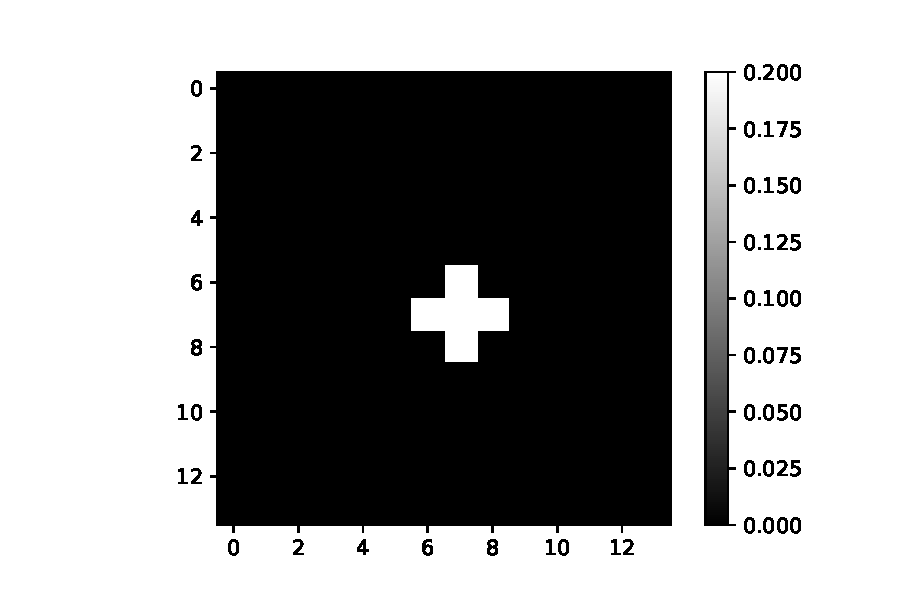
\includegraphics[width=0.27\textwidth]{figs/graph_conv_kernel_im.pdf}
        &
        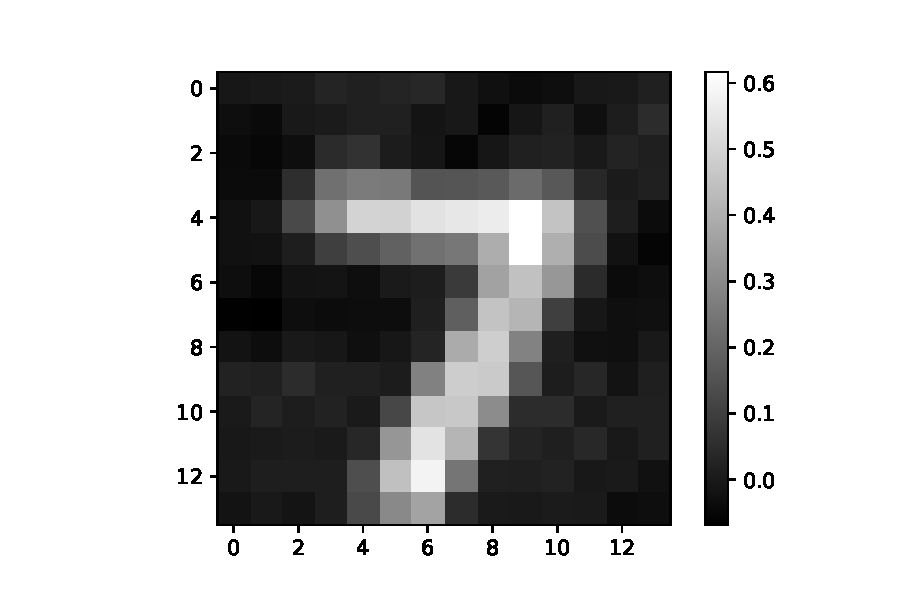
\includegraphics[width=0.27\textwidth]{figs/graph_conv_out_im.pdf} \\
        Input graph/image & Convolutional filter & Output graph/image \\
    \end{tabular}
    \caption{Example of the graph convolution operation for a single graph and single filter.}
    \label{fig:graph_conv}
\end{figure}


\vspace{-3pt}
\paragraph{Extensions of \gnns.}
\gnns were first proposed as early as in 1997 by~\citet{sperduti1997supervised} and subsequently integrated with recurrent neural networks in~\citep{gori2005new,scarselli2008graph}.
The works of~\citet{defferrard2016convolutional} and~\citet{kipf2016semi} synergized with deep learning and the \gnns field has grown considerably.
Notable extensions include Graph Attention Networks~\citep{velickovic2017graph} that learn pairwise attention between nodes to better capture regularities in graphs. Graph Isomorphism Networks~\citep{xu2018how} and Principal Neighbourhood Aggregation~\citep{corso2020principal} use novel more expressive feature aggregation strategies to better differentiate graphs and showed one of the best results in a large-scale graph benchmark~\citep{hu2020open}. Simple GCNs~\citep{wu2019simplifying} propose a single layer \gnn that is computationally efficient yet performant in many tasks. 
Message Passing Networks~\citep{gilmer2017neural,battaglia2018relational} generalize \gnns to support edge features in addition to node features. 
Gated \gnns~\citep{li2015gated} extended earlier \gnns~\citep{gori2005new,scarselli2008graph} based on recurrent networks and recently showed top results among other \gnns in different tasks~\citep{dwivedi2020benchmarking}.

\vspace{-3pt}
\paragraph{Applications of \gnns.} \gnns primarily focus on solving node and graph classification tasks and link prediction~\citep{hamilton2017representation,wu2020comprehensive,battaglia2018relational}. Graph generation~\citep{you2018graphrnn,liao2019efficient} and analysis of dynamic graphs~\citep{kazemi2019relational,trivedi2019dyrep} are also becoming common tasks. Graphs can be used to model virtually any kind of data, so besides solving classic graph tasks such as molecule classification~\citep{xu2018how,knyazev2018spectral}, \gnns have been recently applied to more diverse tasks: image classification~\citep{knyazev2019image,meyer2020large}, semantic segmentation~\citep{li2018beyond,zhang2019dual}, visual relationship detection~\citep{xu2017scene,yang2018graph}, modelling neural network architectures~\citep{zhang2018graph,wen2020neural}, program synthesis~\citep{zhang2018neural}, learning interactions between elements of complex systems~\citep{kipf2018neural,bapst2019structured} and many other tasks. Such a wide range of tasks shows a great potential of \gnns and, therefore, \gnns are a central focuses of this thesis.\looseness-1

\paragraph{Alternatives to \gnns.} Recently, Transformers~\citep{vaswani2017attention,dosovitskiy2020image} have become competitive in diverse tasks. In principle, these models are capable of capturing graph-structured data if the relational information is properly modelled. For example, if relative positional encoding is used~\citep{shaw2018self}, Transformers can learn a graph representation similar to such \gnns as GATs~\citep{velickovic2017graph}. The relation between Transformers and \gnns has been more formally confirmed in~\citep{dwivedi2020generalization,yun2019graph}.


\paragraph{Graph pooling.} Like \cnns, \gnns can exploit the local structure of data to perform some type of downsampling or pooling of the input graph.
In \gnns, pooling methods generally follow the same idea as in \cnns. However, in \gnns the pooling regions (sets of nodes) are often found based on clustering, since there is no regular grid as in images~\citep{defferrard2016convolutional,shaham2018spectralnet,ying2018hierarchical}.
Differently from clustering-based graph pooling, top-k pooling was proposed~\citep{graphunet2018}. Instead of clustering ``similar'' nodes, top-k propagates only part of the input disregarding the rest.
%Top-k pooling can thus select some part of the input graph disregarding the rest. 
%For this reason at first glance it does not appear to be logical.
Formally, given node features $\X^{(l)}$ for layer $l$, the output node features $\mathbf{Z}^{(l)}$ of top-k pooling can be defined as:\looseness-1
%However, we can notice that pooled feature maps in~\cite[Eq.~2]{graphunet2018} are computed in the same way as attention outputs $\mathbf{Z}$ in Eq.~\ref{eq:attn} above, if we rewrite their Eq.~2 in the following way:
%
\begin{equation}
%\label{eq:top-k}
%	Z_i = \alpha_i X_i, \forall i \in P, Z_i = \emptyset, \forall i \notin P
%\[
\mathbf{Z}^{(l)}_i =
\begin{cases}
\mathbf{a}_i \X^{(l)}_i,& \forall i \in P\\
\emptyset, & \text{otherwise} ,
\end{cases}
%\]
\end{equation}
%
where $P$ is a set of indices of pooled nodes, $|P| \leq N$, and $\emptyset$ denotes the unit is absent in the output. $\mathbf{a} \in \R^N$ is predicted by some auxiliary subnetwork: $\mathbf{a}=f(\X^{(l)}, \A)$, where for $f$ a \gnn can be used as in~\citep{lee2019self} or an MLP ignoring the graph structure (adjacency matrix $\A$) can be used as in~\citep{graphunet2018}.
The indices $P$ are the indices of the $|P|$ largest (top) values in $\mathbf{a}$.

Both \gnns and \cnns are built by stacking convolutional and pooling layers to form a deep network. Sometimes, \cnns are augmented with \gnns to improve learning in visual tasks~\citep{li2018beyond,liu2020non}.\looseness-1

\section{Compositional and graph reasoning\label{sec:bg_comp}}

With the basic building blocks, MLPs, \cnns and \gnns, we can build systems that solve complex \textit{compositional reasoning} tasks. In this thesis, by compositional reasoning we assume the process of making a decision by analyzing the collection, or \textit{composition}, of entities where the entities can refer to graph nodes and edges; objects, object parts and relations; or abstract concepts or patterns (\eg subgraphs, strokes, stripes).
In this section, we will describe compositional reasoning methods that mainly concern vision tasks, since these tasks are well studied and easy to understand with simple examples. But similar tasks and methods solving them exist in different domains of compositional reasoning, such as graph reasoning~\citep{hamilton2018embedding} or natural language processing~\citep{lake2018generalization}.\looseness-1

A classic example of compositional visual reasoning is visual question answering (VQA)~\citep{antol2015vqa}. In VQA, the decision is the answer obtained by visually reasoning over a set of objects and relationships between them given a question, \eg \textit{how many chairs are on the left of the table in this image?}. Simpler tasks such as classifying images can also be considered as visual reasoning tasks. Visual reasoning methods may be grouped into low-level and high-level ones and different methods are used in each case. 
%The methods proposed in \S~\ref{sec:completed} and \S~\ref{sec:proposal} will concern both of these groups and, in fact, will be aimed to bridge the gap between them in the context of a specific problem -- compositional generalization.\looseness-1

\subsection{Low-level compositional reasoning\label{sec:bg_low}}
% Explain image classification as a low-level reasoning
We can view image classification as a low-level visual reasoning task, since the model needs to recognize low-level components and relate them to each other in order to make an accurate prediction.
%the category of the object in an image
The low-level components can be object attributes and parts, parts of parts, or even individual pixels.
%in case of tasks such as MNIST~\citep{lecun1998gradient} . 
Reasoning over object parts and attributes rather than making a direct decision about an image enables more explainable decisions~\citep{ul2019explaining} and zero-shot object classification~\citep{lampert2013attribute,demirel2017attributes2classname,naeem2021learning,tokmakov2019learning}. 
For example, a relatively complex zebra image can be recognized if the model detects stripes, a tail, a head, long legs (\fig{\ref{fig:attrib}}a). A simple MNIST image can be recognized based on the composition of strokes and other patterns (\fig{\ref{fig:attrib}}b).
Regardless of image complexity, the lowest level of reasoning is individual pixels. In complex images, the compositions of individual pixels are less likely to directly lead to a particular semantic decision. However, individual pixels can still affect the prediction of object parts and attributes, which in turn can affect the final prediction. Therefore, it is important to consider low-level reasoning both in simple and complex images to develop more robust and explainable models.\looseness-1
%compared to simple images. 
%So in complex images, low-this form of reasoning is rather abstract. 
%Since this reasoning still affects the final decision, it can be called ``hidden'' reasoning. Low-level reasoning includes all these different forms of reasoning.
%\paragraph{Hidden reasoning}
%By low-level reasoning we will also assume pixel level reasoning that does not directly lead to a particular decision. Maybe call this hidden reasoning?


\begin{figure}[htbp]
    \centering
    \setlength{\tabcolsep}{10pt}
    \begin{tabular}{cc}
         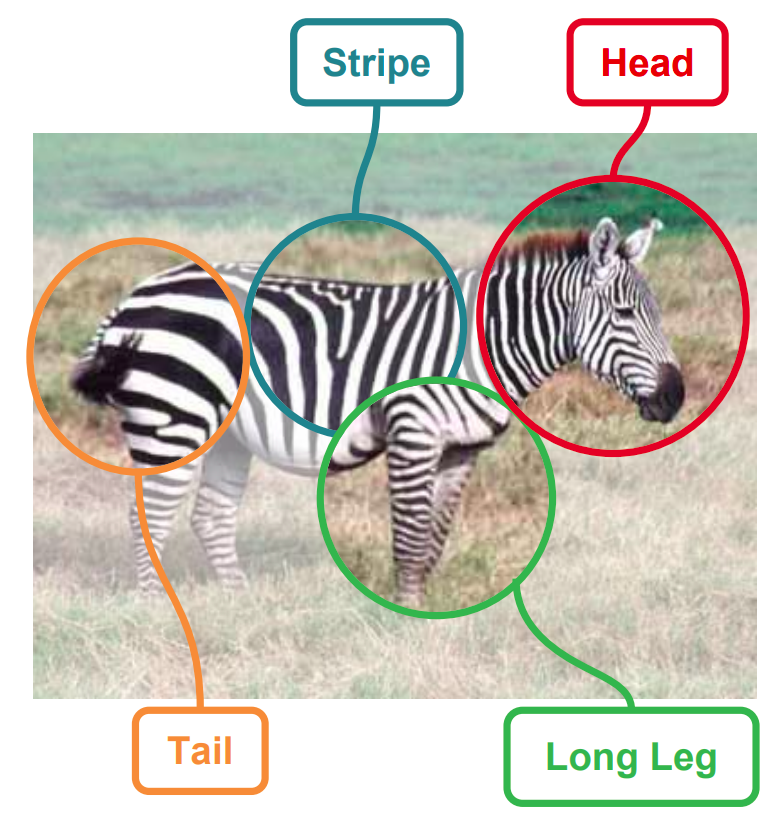
\includegraphics[width=0.3\textwidth,align=c]{figs/zebra_atrib.png}
         & 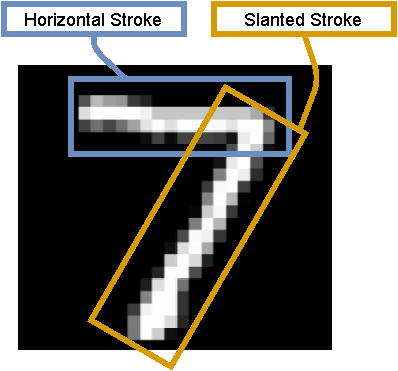
\includegraphics[width=0.3\textwidth,align=c]{figs/mnist_atrib.pdf} \\
         (a) & (b)
    \end{tabular}
    \vspace{-5pt}
    \caption{ (a) A zebra can be described as a collection of object parts, patterns and attributes (figure from~\citep{demirel2017attributes2classname}); (b) A digit can be described as a collection of primitive strokes and patterns.}
    \label{fig:attrib}
    \vspace{-10pt}
\end{figure}

\subsection{High-level compositional reasoning\label{sec:bg_high}}
\vspace{-3pt}

High-level visual reasoning has been more extensively  studied in different tasks than low-level reasoning. The most common, and perhaps, comprehensive high-level reasoning task is Visual Question Answering (VQA)~\citep{antol2015vqa,johnson2017clevr}. One of the ways to effectively solve VQA is to first extract a semantic image description -- a scene graph~\citep{NSM2019,yi2018neural,zhang2019empirical}. 
Formally, a scene graph~\citep{johnson2015image} ${\cal G}=(O,R)$ consists of a set of subjects and objects ($O$) as nodes and a set of relationships or predicates ($R$) between them as edges. The nodes and edges form visual relationship \textit{triplets}: $\langle$\textit{subject}, \textit{predicate}, \textit{object}$\rangle$, \eg
% $\langle$person, on, surfboard$\rangle$, 
$\langle$cup, on, table$\rangle$. %Each node in the graph corresponds to a subject or object (with a specific image location) and edges correspond to predicates. 
%Besides bridging the gap, SGs can be used to verify how well the model has understood the visual world, as opposed to just exploiting one of the biases in a dataset~\citep{jabri2016revisiting,anand2018blindfold,bahdanau2018systematic}.
% Thus, scene graphs are semantic descriptions of images. 
Solving VQA becomes much easier when the input to the question-answering module is semantic, such as a scene graph, rather than raw pixels or abstract features. Similar to VQA, in image captioning~\citep{yang2019auto, gu2019unpaired} and retrieval~\citep{johnson2015image,belilovsky2017joint,tang2020unbiased}, extracting a scene graph from images also simplifies the task improving the downstream performance. Inferring a scene graph is also beneficial for explainable visual reasoning~\citep{shi2019explainable} within the explainable AI (XAI) paradigm~\citep{gunning2019darpa}, since the final predictions can be traced back to semantic concepts of scene graphs.
Extracting a scene graph generally requires a predefined vocabulary of concepts, which is a time-consuming process that must be done for each new task. Therefore, a more flexible strategy is to describe images using abstract entities~\citep{norcliffe2018learning,vedantam2019probabilistic,locatello2020object,burgess2019monet,greff2020binding} that, if necessary, can be tied to semantic concepts (see \S~\ref{sec:bg_methods}).\looseness-1
% -- a semantic collection of objects and relationships between them. 
%As reasoning over abstract entities is not necessary high-level, so the corresponding methods are reviewed separately in § 3.2.4.
% \begin{figure}[thbp]
% 	\centering
% 	\begin{scriptsize}
% 		\setlength{\tabcolsep}{1pt}
% 		\begin{tabular}{c} 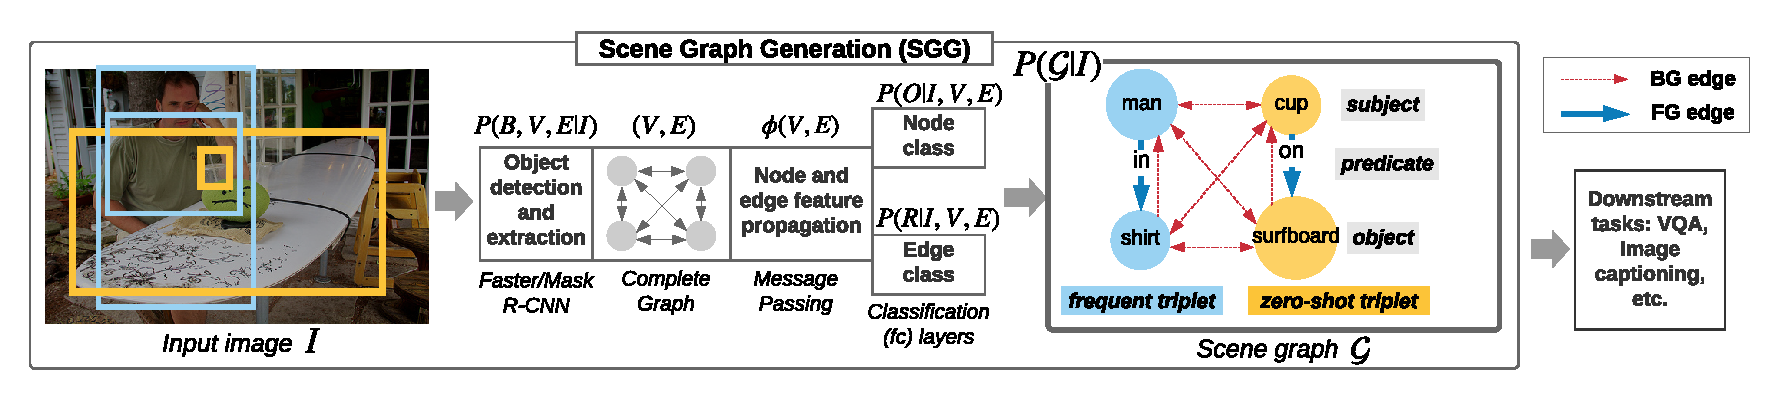
\includegraphics[width=0.99\textwidth,align=c,trim={0 0.2cm 0 0.2cm},clip]{2020_bmvc/figs/cup_on_surfboard_overview1.pdf} \\
% 		\end{tabular}
% 	\end{scriptsize}
% 	\vspace{-5pt}
% 	\caption{\small Typical scene graph generation pipeline used in high-level visual reasoning tasks (figure from~\citep{knyazev2020graph}). Foreground (FG) edges denote annotated relations, while background (BG) ones denote the absence of relations as deemed by the annotator or annotation system.} %In many downstream tasks, such as VQA, the result directly depends on the accuracy of predicted scene graphs.}
% 	\label{fig:overview_sg}
% \end{figure}

\begin{figure}[thbp]
	\centering
	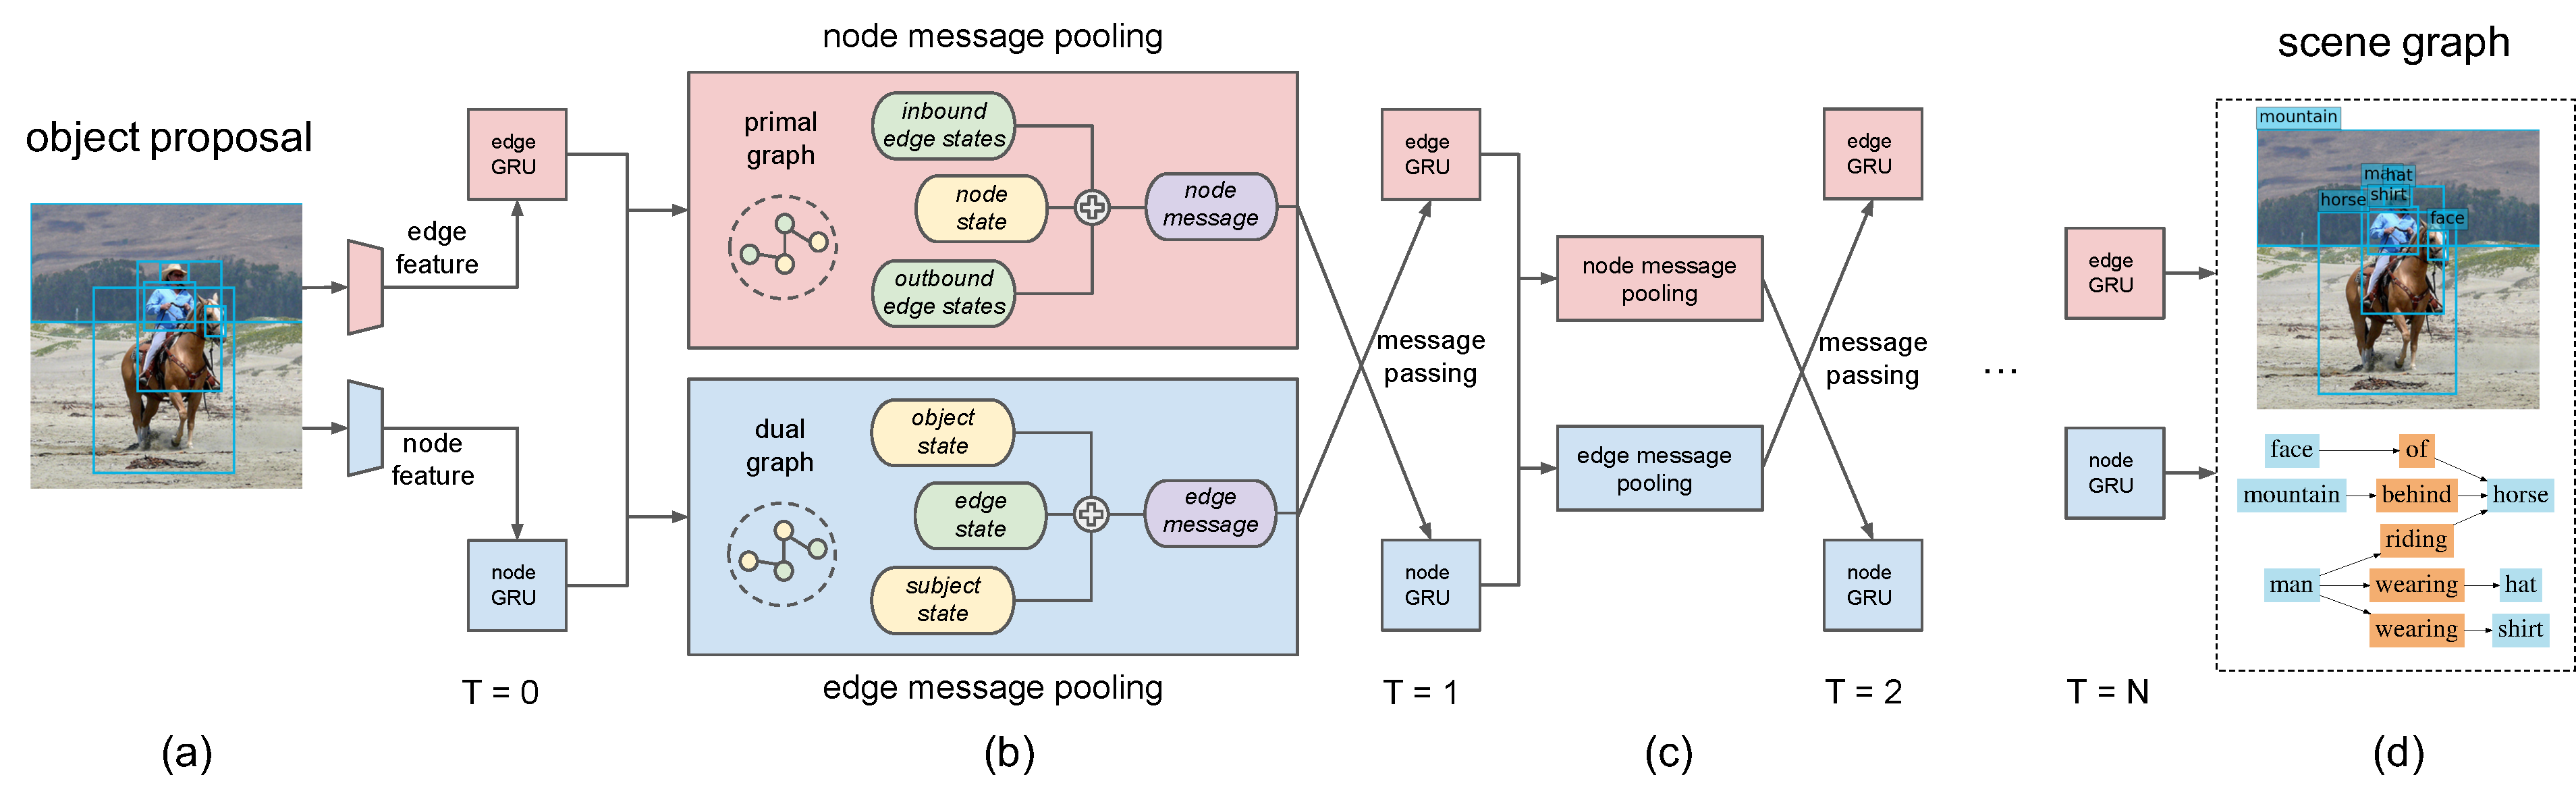
\includegraphics[width=0.99\textwidth,align=c,trim={0 2.1cm 0cm 0.2cm},clip]{figs/stanford_network.pdf}
	%\vspace{-5pt}
	\caption{\small A scene graph generation model from~\citep{xu2017scene} used in high-level visual reasoning tasks. This and other SGG models~\citep{yang2018graph} are often based on message passing networks that resemble graph neural networks~\citep{gilmer2017neural,battaglia2018relational}.}
	\label{fig:overview_sg}
\end{figure}

%In scene graph generation} (SGG) the task is to predict a scene graph (SG) given an input image. %The inferred SG can be used directly for downstream tasks such as VQA~\citep{zhang2019empirical,NSM2019}, image captioning~\citep{yang2019auto, gu2019unpaired} or retrieval~\citep{johnson2015image,belilovsky2017joint,tang2020unbiased}.
%A model which performs well on SGG should demonstrate the ability to ground visual concepts to images and generalize to compositions of objects and predicates in new contexts.
% \paragraph{Overview of Scene Graph Generation}
% 	\label{sec:baseline}
Extracting a scene graph $\cal G$ from an image $I$ is a standard high-level visual reasoning task and is called scene graph generation (SGG)~\citep{xu2017scene}. In general, SGG models first extract a complete graph from an image, where nodes correspond to detected objects~\citep{zellers2018neural,yang2018graph}. Then several message passing rounds update node and edge features. The goal of the SGG model is to predict a sparse scene graph $\cal G$ given the dense graph of node and edge features (\fig{\ref{fig:overview_sg}}).
Typically, many different $\cal G$ can be valid for a single image $I$, so obtaining $\cal G$ resembles a generative process. However, in practice there is typically only one ground-truth $\cal G$ annotated for each image and the SGG models are typically deterministic, so the task is rather ``scene graph prediction''. Nevertheless, we will use the term SGG to be consistent with the scene graph literature.


\subsection{Compositional generalization\label{sec:bg_comp_gen}}

In real world images, some compositions, \eg~$\langle$cup, on, table$\rangle$ or $\langle$person, on, surfboard$\rangle$, appear more frequently than other unusual ones, \eg~$\langle$cup, on, \textit{surfboard}$\rangle$, $\langle$cup, \textit{under}, table$\rangle$ or $\langle$\textit{dog}, on, surfboard$\rangle$. %, which creates a strong frequency bias. 
Such a difference in frequencies -- the \textit{frequency bias} -- is often present in commonly-used visual relationship datasets, such as Visual Genome~\citep{krishna2017visual}.
% (\fig{\ref{fig:motivation_gan}}). 
The frequency bias is purely statistical and poorly reflects the physical plausibility of object interactions. For example, according to the statistics of Visual Genome the probability of $\langle$cup, on, {surfboard}$\rangle$ is exactly zero because such a composition has never occurred. However, from the physical point of view (in the real world), such a composition would have a greater than zero probability. In fact, $\langle$cup, on, {surfboard}$\rangle$ appears in the test set of Visual Genome.
%of  and are often called the frequency bias.
The ability of models to recognize such novel (\textit{zero-shot} or ZS) and rare (\textit{few-shot} or FS) compositions accurately, despite the frequency bias, is called \textit{\cg} (\cgshort). 
Compositional generalization has been widely studied in the language~\citep{atzmon2016learning, keysers2019measuring, lake2019compositional} and reinforcement learning domains~\citep{jiang2019language,cogswell2019emergence,kipf2019compile}, as well as multi-domain tasks~\citep{johnson2017clevr,bahdanau2018systematic,bahdanau2019closure,agrawal2017c,agrawal2018don}.
In the visual domain, compositional reasoning has been addressed in the scene graph generation (SGG) task and image classification from attributes~\citep{lampert2013attribute,demirel2017attributes2classname,naeem2021learning} (\fig{\ref{fig:zeroshots}}).

\begin{figure}[thbp]
	\centering
	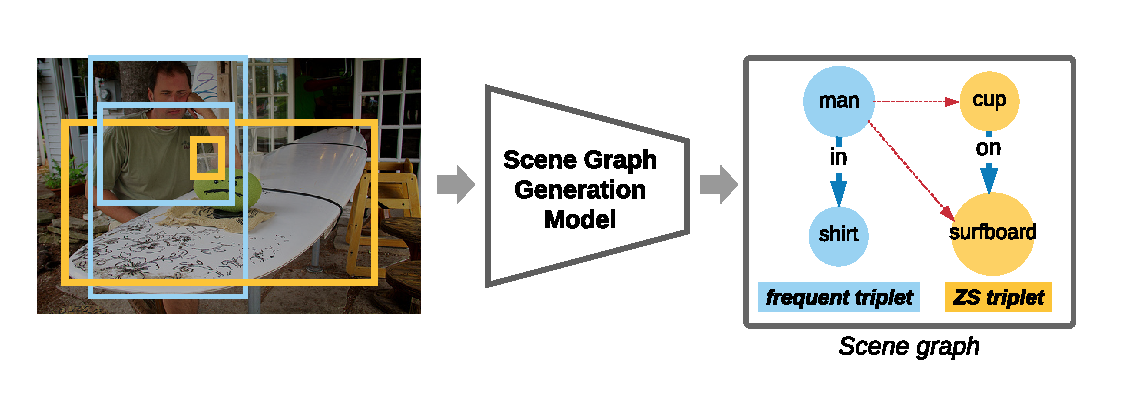
\includegraphics[width=0.99\textwidth,align=c,trim={0 0cm 0cm 0cm},clip]{figs/zeroshots.pdf}
	\vspace{-15pt}
	\caption{\small An example of a ground truth scene graph with a zero-shot composition (ZS triplet) that must be predicted by an SGG model for an input image. The figure is adapted from~\citep{knyazev2020graph}. Dashed red arrows denote the relationships that have not been annotated by a human.}
	\label{fig:zeroshots}
\end{figure}

%So, unless the models have a strong inductive prior , they will tend to predict `person' rather than `dog' on a surfboard. 
While compositional reasoning about concepts is easy for humans, for machines this task has remained extremely challenging. 
The reasons for the challenging nature of \cgshort are not well understood.
The challenge may relate to the fact that learning-based models tend to capture spurious statistical correlations and biases of datasets during training~\citep{arjovsky2019invariant,niu2020counterfactual,tang2020unbiased}. 
%The frequency bias of visual relationship datasets is particularly pronounced making it hard for the models to recognize relationships without relying on the bias.
The frequency bias of visual relationship datasets is particular pronounced, so for the learning-based models it is hard to not rely on this bias.
%The presence of the strong frequency bias in data and the tendency of models to rely on this bias make the \cgshort problem extremely challenging.
The \cgshort challenge has been largely overlooked, since the test sets often have the same frequency bias and the evaluation metrics do not penalize models for blindly relying on the bias. However, when the evaluation is explicitly focused on \cgshort, the models have been found to fail remarkably~\citep{atzmon2016learning, lu2016visual, tang2020unbiased, knyazev2020graph}.

In the SGG task, recall-based metrics are typically used for evaluation. So, on frequent compositions these metrics can reach $\sim$41\%, while on zero-shot compositions the state-of-the-art result is only 4.5\% -- a nearly 10 fold drop in performance~\citep{tang2020unbiased}.
Previous SGG works often assume \cgshort is similar to few-shot predicate generalization and so attempt to improve mean (or predicate-normalized) recall metrics that are not directly related to \cgshort~\citep{chen2019knowledge, dornadula2019visual,tang2019learning,zhang2019graphical,tang2020unbiased,chen2019scene,zareian2020bridging,yan2020pcpl}.  
Predicate imbalance can be treated by simple resampling-based methods, while \cgshort is more challenging~\citep{tang2020unbiased}. Therefore, \cgshort rather than predicate imbalance has to be a focus of visual reasoning tasks.


\subsection{Methods to improve compositional generalization\label{sec:bg_methods}}

The methods to improve visual \cg (\cgshort) can be grouped into two categories. These are: methods that explicitly impose some compositional inductive prior on the models, and those where \cgshort comes, or can potentially come, as a side-effect. The side-effect can be, for example, a result of a regularization method applied to neural networks.\looseness-1

\paragraph{Explicit Compositionality.}
Methods to introduce explicit compositionality can be grouped into high-level and lower-level reasoning tasks. The works on other forms of generalization related to high-level \cg are also discussed.

\begin{itemize}[leftmargin=5mm]
    \item \textbf{High-level visual reasoning}: High-level visual \cgshort was first evaluated in~\citep{lu2016visual} on the VRD dataset using a joint vision-language model.
    Several follow-up works attempted to improve upon it: by learning a translation operator in the embedding space~\citep{zhang2017visual}, clustering in a weakly-supervised fashion~\citep{peyre2017weakly}, using conditional random fields~\citep{cong2018scene} or optimizing a cycle-consistency loss to learn object-agnostic features~\citep{yang2018shuffle}. Augmentation using generative models to synthesize more examples of rare compositions is another promising approach~\citep{wang2019generating}, because we can generate many instances of rare compositions mitigating the frequency bias. 
    But, in \citep{wang2019generating} this approach was only evaluated on a simple predicate classification task.
    %In our work, we also consider subject/object classification to enable the classification of the whole triplets, making the ``image to scene graph'' pipeline complete. 
    Most recently,~\citet{tang2020unbiased} proposed to mitigate the bias by inferring causal rather than correlated relationships and, consequently, showed strong performance on zero-shot visual compositions. In a subsequent work, \citet{suhail2021energy} improved the SGG loss function \eqref{eq:scene_graph_prob_simple} to reduce the bias and better handle \cgshort.
    %In the visual domain, compositionality has been introduced in the form of translation operators~\citep{zhang2017visual}, decoupling object and predicate features~\citep{yang2018shuffle} and constructing causal graphs~\citep{tang2020unbiased}.
    In the VQA task, compositionality has been improved by predefining neural modules~\citep{andreas2016neural} and their more flexible end-to-end extensions \citep{hu2017learning,johnson2017inferring}.
    However, since the VQA task often relies on accurately extracting scene graphs, the methods that impose a compositional prior on scene graph prediction improve \cgshort in VQA~\citep{yi2018neural,mascharka2018transparency,shi2019explainable}.
    
    \item %Explicit compositionality has been introduced in lower-level reasoning tasks such as image and attribute classification. 
    \textbf{Lower-level visual reasoning}: The area of low-level visual reasoning is less organized and there is no standard evaluation benchmark. So different works have focused on different aspects of compositionality at the level of simple objects, object parts and attributes. In particular, to improve compositionality of simple objects, a mask-based loss term was added to image classification networks in~\citep{stone2017teaching}. However, this loss requires expensive pixel-wise mask annotations for training images. 
    %However, the loss was shown to improve compositionality.
    In another work~\citep{sylvain2019locality}, to improve generalization to unseen object categories, a more local representation using self-supervised objectives based on Deep InfoMax~\citep{hjelm2018learning} was learned. 
    %To recognize novel object categories, compositional understanding at the level of object parts and attributes is essential.
    Zero-shot object classification was also studied in~\citep{tokmakov2019learning}. The model in \citep{tokmakov2019learning} is based on decomposing the image representation into a set of attribute representations in the visual space. However, the model does not require to annotate attributes for novel classes to predict their labels.
    Generalization to zero-shot objects and object-attribute compositions may be approached by learning an image extraction \cnn together with a \gnn that learns a knowledge graph from existing object categories and their attributes~\citep{naeem2021learning}. 
    Another approach to this task is based on a prototypical model that learns object representations disentangled from attribute representations to enable strong generalization to unseen compositions of objects and attributes~\citep{ruis2021independent}. To further progress in the lower-level \cgshort, more standardized benchmarks are needed. Integration of the lower-level and higher-level \cgshort methods and evaluation protocols can also enable faster progress towards better generalization in visual reasoning.
    
    \item \textbf{Other tasks}: Several general methods exist that can be potentially useful for \cgshort. One such method is unsupervised domain adaptation (UDA) by backpropagation~\citep{ganin2015unsupervised} closely connected to domain-adversarial neural networks\citep{ajakan2014domain,JMLR:v17:15-239}. UDA achieved strong results by learning features invariant to the domain. Such a model allows to recognize objects in novel domains and contexts.
    Another general method is meta-learning~\citep{hospedales2020meta} that typically targets few-shot generalization in classification tasks. 
    The idea of commonly-used meta-learning methods, such as MAML~\citep{finn2017model}, is to take the original training dataset and split it into a sequence of training and validation subsets (episodes). The critical part is to make the validation set largely composed of few-shot data. This way, the meta-learning algorithm aims to update the parameters of a model on the validation loss thereby improving it by learning to generalize to a few examples. In compositional language reasoning, such a meta-learning based objective was proposed in~\citep{lake2019compositional}, where the validation set is largely composed of zero and few shot compositions. This method yielded improvement \cgshort on language tasks, and potentially, can be applied to visual tasks.
\end{itemize}


\paragraph{Implicit Compositionality via Object-centric Learning.}

Unsupervised learning has recently received more attention in different visual tasks~\citep{radford2015unsupervised,hjelm2018learning,chen2020simple,verma2021towards}, and is potentially useful for \cgshort as well.
In particular, one of the reasons for poor \cgshort of models might be the biased annotations in the datasets on which models are trained. Therefore, a logical way to mitigate such bias is to rely less on the annotations. In an extreme case, we can train a model without any labels, in a purely unsupervised fashion.
In the context of compositional visual reasoning, a growing body of unsupervised learning works focus on object-centric learning~\citep{greff2020binding}, usually by employing an encoder-decoder model~\citep{engelcke2019genesis,burgess2019monet,greff2019multi,locatello2020object}.
Object-centric learning methods generally decompose an image representation into a set of object representations without accessing the labels of the objects. Some methods also allow to disentangle physical attributes of objects, such as color, shape and material~\citep{greff2019multi}. The decomposition of an image into objects is typically done by iteratively running encoder-decoder inference until the image is fully reconstructed~\citep{greff2019multi}. 
%The method in~\citep{greff2019multi} allows to not only separate objects from each other, but also to disentangle objects from their physical attributes. 
Due to its iterative nature, the inference procedure is computationally inefficient.
Another method, slot attention~\citep{locatello2020object}, is more efficient, since it only requires a single encoder iteration to extract all object representations. Yet, it is unclear if this model disentangles object attributes as in~\citep{greff2019multi}. Slot attention is reminiscent to the k-means clustering method. Unlike k-means, slot attention is fully-differentiable and employs self-attention~\citep{vaswani2017attention} with the softmax function to enforce more sparse representation. Object-centric learning methods are typically evaluated using pixel-wise segmentation metrics similar to earlier unsupervised semantic segmentation works~\citep{arbelaez2010contour}.
In addition, in \citep{locatello2020object,greff2019multi} the evaluation includes how well the representation encodes visual object properties.
Overall, object-centric learning is a promising direction for \cgshort as it enables an unbiased (w.r.t. human annotations) decomposition of images into entities that often have a semantic meaning. Such unbiased decomposition recently allowed object-centric learning methods to improve results on several out-of-distribution generalization tasks~\citep{dittadi2021generalization}.\looseness-1

\paragraph{Implicit Compositionality via Regularized Training.}

Regularization methods are often aimed at reducing overfitting and improving different generalization abilities. An open question remains whether or not these methods can also improve \cgshort.
% Among the regularization methods to reduce overfitting and improve overall generalization, 
In the following, the methods that can be more directly leveraged for compositional generalization are considered.

Let us consider the feature activations after some layer $l$: $\X^{(l)} \in \R^{N \times d_l}$, where 
$N$ is the number of data points (in a batch) and
%$n \in [1, N]$ is an index of a sample in the batch of $N$ sample and 
$d_l$ is dimensionality\footnote{$\X^{(l)}$ can be outputs of a fully-connected, convolutional, graph layer, etc. In the case of 2D or 3D dimensions in $\X^{(l)}$, such as after convolutions, it can be flattened to a 1D tensor.\looseness-1}. 
To index the $i$-th individual feature (scalar) of the $n$-th sample, the notation $\X_{n,i}$ will be used.
In the visual domain, when a \cnn is used to extract $\X$, these activations tend to be highly-correlated due to the regularities in the input data and co-adaptation of weights to capture those regularities~\citep{hinton2012improving}, \ie the probability $p(\X_{n,i} | \X_{n,j})$ tends to be high. For example, if the $i$-th feature is activated when the input image contains `surfboard', then the $j$-th feature associated with the entity `person' is likely to be activated regardless if the image actually contains the `person' or another object such as `dog'. On the one hand, relying on co-adaptation allows neural networks to fit data more easily. %similarly as relying on (spurious) context in %high-level visual reasoning. 
On the other hand, heavy reliance on co-adaptation can hurt generalization, so some regularization strategies are needed to mitigate that.\looseness-1

Many regularization strategies to alleviate overfitting have been proposed. One common strategy is Dropout~\citep{hinton2012improving}: $\text{dropout}(\X, r)$. Dropout stochastically sets to zero the values of $\X$ with probability $r$ during training. \citet{ghiasi2018dropblock} generalized this method to convolutions by setting to zero locally connected activations rather than arbitrary ones.
In contrast, \citet{cogswell2015reducing} proposed a covariance loss penalty to explicitly reduce correlation of features.
Adding the loss penalty to the task objective helped the networks to obtain better generalization properties compared to using Dropout. 
However, due to the expensive procedure of computing covariance, this approach does not scale well to high-dimensional features typically present in visual tasks. 
This limitation was addressed by introducing a locally connected decorrelation penalty specific for convolutional features~\citep{rodriguez2016regularizing}.
Instead of adding a loss penalty~\citep{cogswell2015reducing,rodriguez2016regularizing}, enforcing orthogonality on weights in \cnns during initialization may help to better regularize the model and, subsequently, achieve better generalization results~\citep{bansal2018can,wang2020orthogonal}. However, it is important to maintain the orthogonality regularization during the whole training procedure, because the weights tend to diverge to a poor solution otherwise~\citep{wang2020orthogonal}. Alternatively, generalization can also be improved using decorrelated batch normalization (BN)~\citep{huang2018decorrelated}, which can also be viewed as a form of regularization. While decorrelated BN improves generalization compared to original BN~\citep{ioffe2015batch}, it remains unclear if decorrelated BN is better for generalization than other regularization strategies, such as orthogonal regularization.\looseness-1

The discussed regularization methods mainly improve generalization results in a more classic machine learning sense, such as generalization to the in-distribution test images.
%, they only address the linear independence of features. Nonlinear correlations and, hence redundancy, can be well present in networks. Moreover,
However, except for a few synthetic experiments in~\citep{cogswell2015reducing}, the effect of these methods on out-of-distribution and, especially, compositional generalization has not been systematically evaluated. Meanwhile, these regularization techniques, in particular the orthogonal one, can facilitate learning a representation where entities are more (linearly) independent, and hence disentangled, from each other. This might directly improve \cgshort, which needs to be empirically confirmed.
  % means the % means the 2019_neurips folder, file folder, file background.tex
\graphicspath{{Ch3_2019_neurips/figs/}}

\chapter{{Understanding Attention and Generalization in Graph Neural Networks}\label{ch:neurips2019}}

%\chapter{PROLOGUE TO FIRST ARTICLE}
\section*{Prologue}
\addcontentsline{toc}{section}{Prologue}

%\hspace{-8pt}
% \begin{tabular}{p{0.16\linewidth}p{0.78\linewidth}}
%      \textit{Title:} & Understanding Attention and Generalization in Graph Neural Networks \\
%      \textit{Authors:} & Boris Knyazev, Graham Taylor, Mohamed Amer \\
%      \textit{Published at:} & \venue{Neural Information Processing Systems (NeurIPS 2019)} \\
%     \textit{Code release:} & \url{https://github.com/bknyaz/graph_attention_pool} \\
%     \textit{Personal contributions:} & developed the key components of algorithms and models; developed the code; designed
% and ran all experiments; wrote most of the article.
% \end{tabular}

\vspace{5pt}
\densepar{Context.}
Graph neural networks (\gnns) are state of the art models for machine learning on graphs (see~\citep{wu2020comprehensive,bronstein2017geometric,hamilton2017representation} for reviews). The downstream performance of \gnns is often improved by learning an attention module deciding which graph substructures are important for a given task~\citep{graphunet2018}. However, prior work on attention has not analyzed if attention learns anything useful about the task or whether the performance improvement is due to other confounding factors associated with adding attention. Compared to more intuitive tasks like image classification, in graph tasks it is often challenging to annotate ground truth about which graph substructures are important for the task. Therefore, it is especially challenging to understand the effect of attention in \gnns.


%\vspace{-3pt}
\densepar{Contributions.}
We developed synthetic tasks where we can easily define ground truth importance of graph substructures for the task. Using these tasks, we found that attention can learn useful patterns about data if attention modules are initialized in a ``good'' way. We also found that the initialization effect is especially pronounced on the generalization ability of \gnns, in particular when evaluated on larger and more noisy graphs compared to the graphs used to train \gnns.
%We show that a strong inductive bias to generalization to larger and noisy graphs can be incorporated by carefully initializing the attention modules of \gnns. 
We show that on real graph datasets, such a ``good'' initialization is hard to achieve. To this end, we provide a simple method that makes attention modules less sensitive to initialization. Consequently, we show improved generalization in several real graph tasks.


%\vspace{-3pt}
\densepar{Recent works.}
The datasets we had introduced in our paper have been subsequently used in recent works~\citep{dwivedi2020benchmarking,vincent2021online,ma2020adaptive,wang2020haar}. Motivated by our work, attention and attention-based pooling in \gnns has been improved to extract graph substructures more accurately~\citep{kim2020find,wang2020haar,ji2020hopgat}.
Evaluating the generalization of \gnns \wrt the graph size and other properties have become common~\citep{velivckovic2019neural,verma2019stability,sinha2020evaluating}.
%While ours and most other works study generalization in \gnns from the empirical view, 
Theoretical generalization bounds for \gnns studied in~\citep{garg2020generalization} complement our empirical results by providing conditions for \gnns generalization.


\section{Attention meets pooling in graph neural networks}\label{sec:attn_intro}

The practical importance of attention in deep learning is well-established and there are many arguments in its favor~\citep{vaswani2017attention}, including interpretability~\citep{park2016attentive, deac2018attentive}.
In graph neural networks (\gnns), attention can be defined over edges~\citep{velickovic2017graph, zhang2018gaan} or over nodes~\citep{lee2018graph}. In this work, we focus on the latter, because, despite being equally important in certain tasks, it is not as thoroughly studied~\citep{lee2018attention}. To begin our description, we first establish a connection between attention and pooling methods.
In convolutional neural networks (CNNs), pooling methods are generally based on uniformly dividing the regular grid (such as one-dimensional temporal grid in audio) into local regions and taking a single value from that region (average, weighted average, max, stochastic, etc.), while attention in CNNs is typically a separate mechanism that weights $C$-dimensional input $\X \in \mathbb{R}^{N \times C}$:
%
\begin{equation}
\label{eq:attn}
\Z = \mathbf{\alpha} \odot \X,
\end{equation}
%
\noindent where $\Z_i = \mathbf{\alpha}_i \X_i$ - output for unit (node in a graph) $i$, $\sum_i^N \mathbf{\alpha}_i = 1$, $\odot$ - element-wise multiplication, $N$ - the number of units in the input (i.e. number of nodes in a graph).

In \gnns, pooling methods generally follow the same pattern as in CNNs, but the pooling regions (sets of nodes) are often found based on clustering~\citep{defferrard2016convolutional, shaham2018spectralnet, ying2018hierarchical}, since there is no grid that can be uniformly divided into regions in the same way across all examples (graphs) in the dataset.
Recently, top-k pooling~\citep{graphunet2018} was proposed, diverging from other methods: instead of clustering ``similar'' nodes, it propagates only part of the input and this part is not uniformly sampled from the input. Top-k pooling can thus select some local part of the input graph, completely ignoring the rest. For this reason at first glance it does not appear to be logical.

However, we can notice that pooled feature maps in~\cite[Eq.~2]{graphunet2018} are computed in the same way as attention outputs $\Z$ in \eqref{eq:attn} above, if we rewrite their Eq.~2 in the following way:
%
\begin{equation}
\label{eq:top-k}
%	\Z_i = \mathbf{\alpha}_i X_i, \forall i \in P, \Z_i = \emptyset, \forall i \notin P
%\[
\Z_i =
\begin{cases}
\mathbf{\alpha}_i \X_i,& \forall i \in P\\
\emptyset, & \text{otherwise} ,
\end{cases}
%\]
\end{equation}
%
where $P$ is a set of indices of pooled nodes, $|P| \leq N$, and $\emptyset$ denotes the unit is absent in the output.

The only difference between \eqref{eq:top-k} and \eqref{eq:attn} is that $\Z \in \mathbb{R}^{|P| \times C}$, i.e. the number of units in the output is smaller or, formally, there exists a ratio $r=|P| / N \leq 1$ of preserved nodes.
We leverage this finding to integrate attention and pooling into a unified computational block of a GNN.
In contrast, in CNNs, it is challenging to achieve this, because the input is defined on a regular grid, so we need to maintain resolution for all examples in the dataset after each pooling layer.
In \gnns, we can remove any number of nodes, so that the next layer will receive a smaller graph. When applied to the input layer, this form of attention-based pooling also brings us interpretability of predictions, since the network makes a decision only based on pooled nodes.

\begin{figure}[t]
	\begin{center}
		\small
		\begin{tabular}{ccc}
			{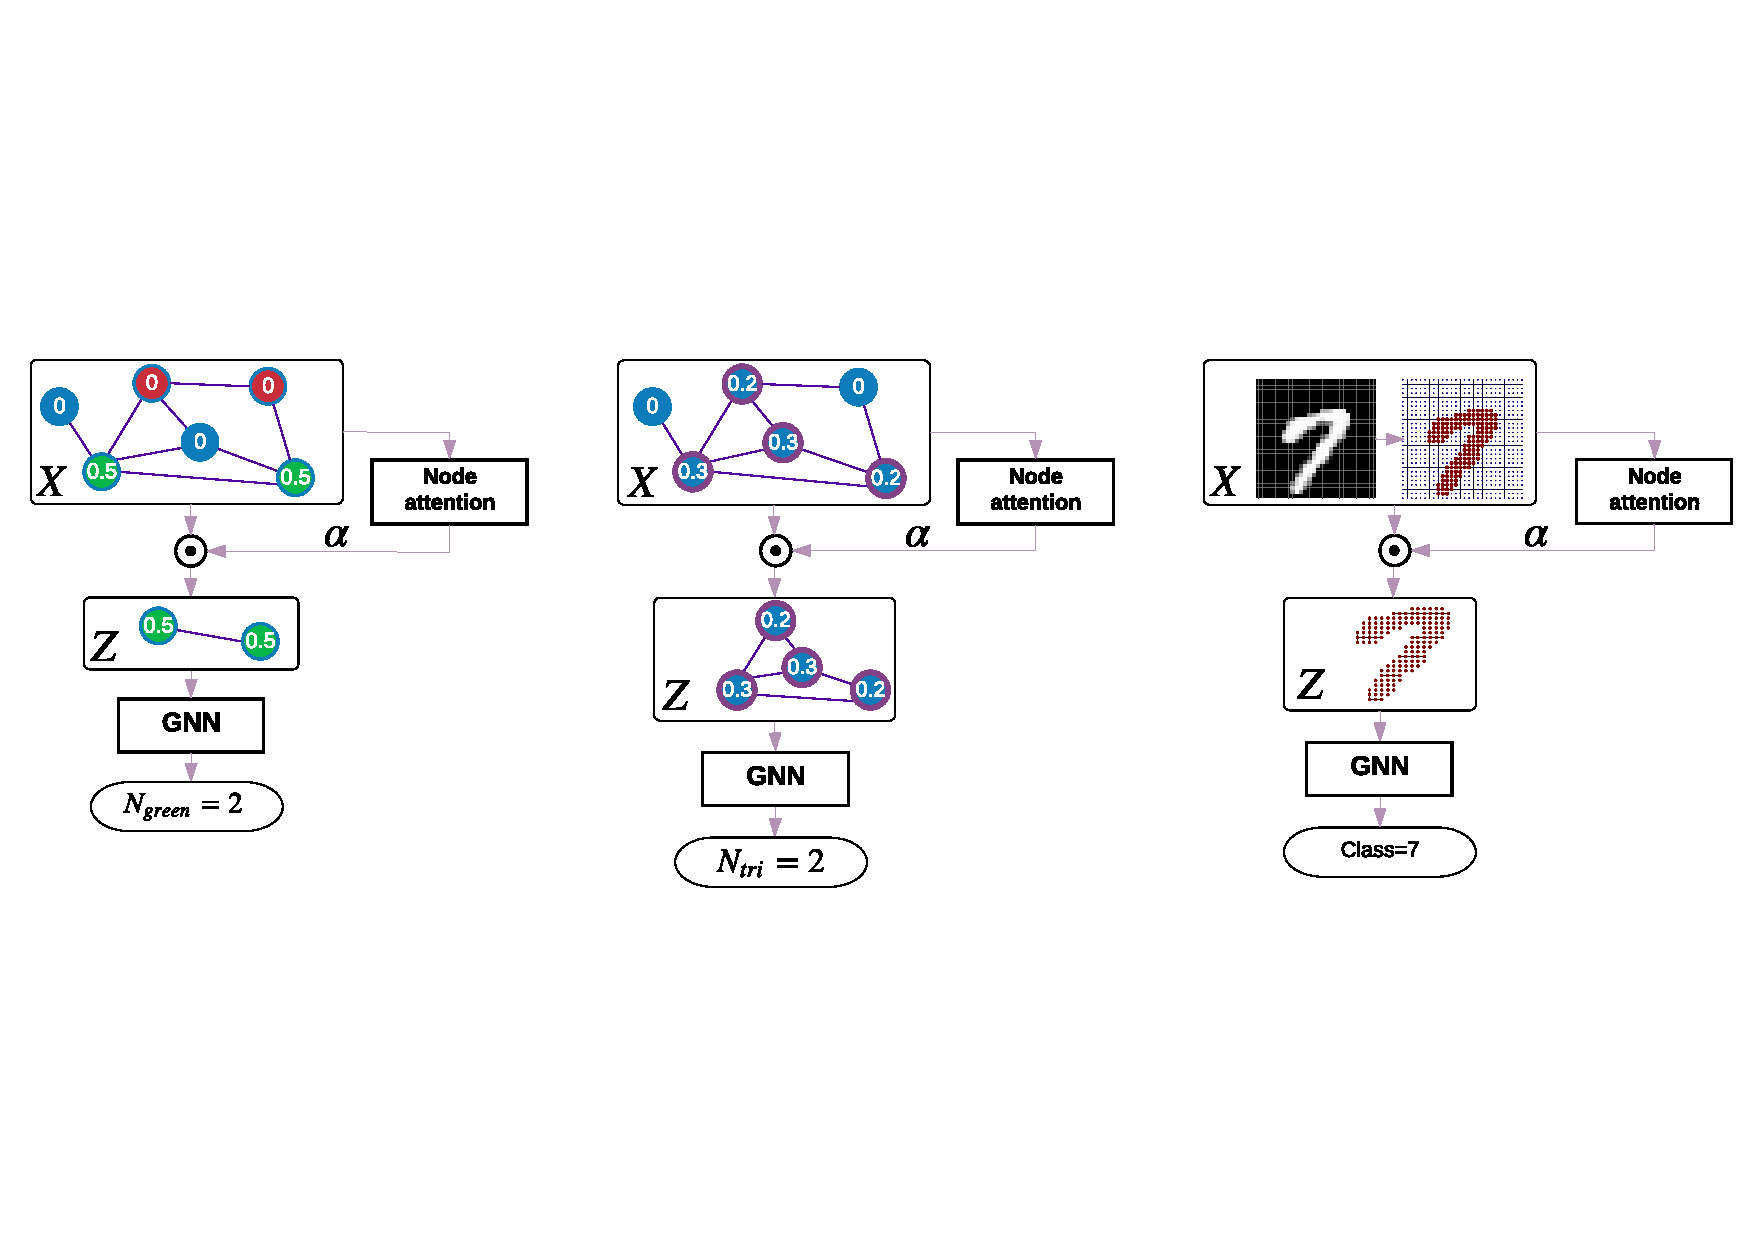
\includegraphics[width=0.3\textwidth, align=c, trim={0cm 6.5cm 20.7cm 6cm}, clip]{tasks}} &
			{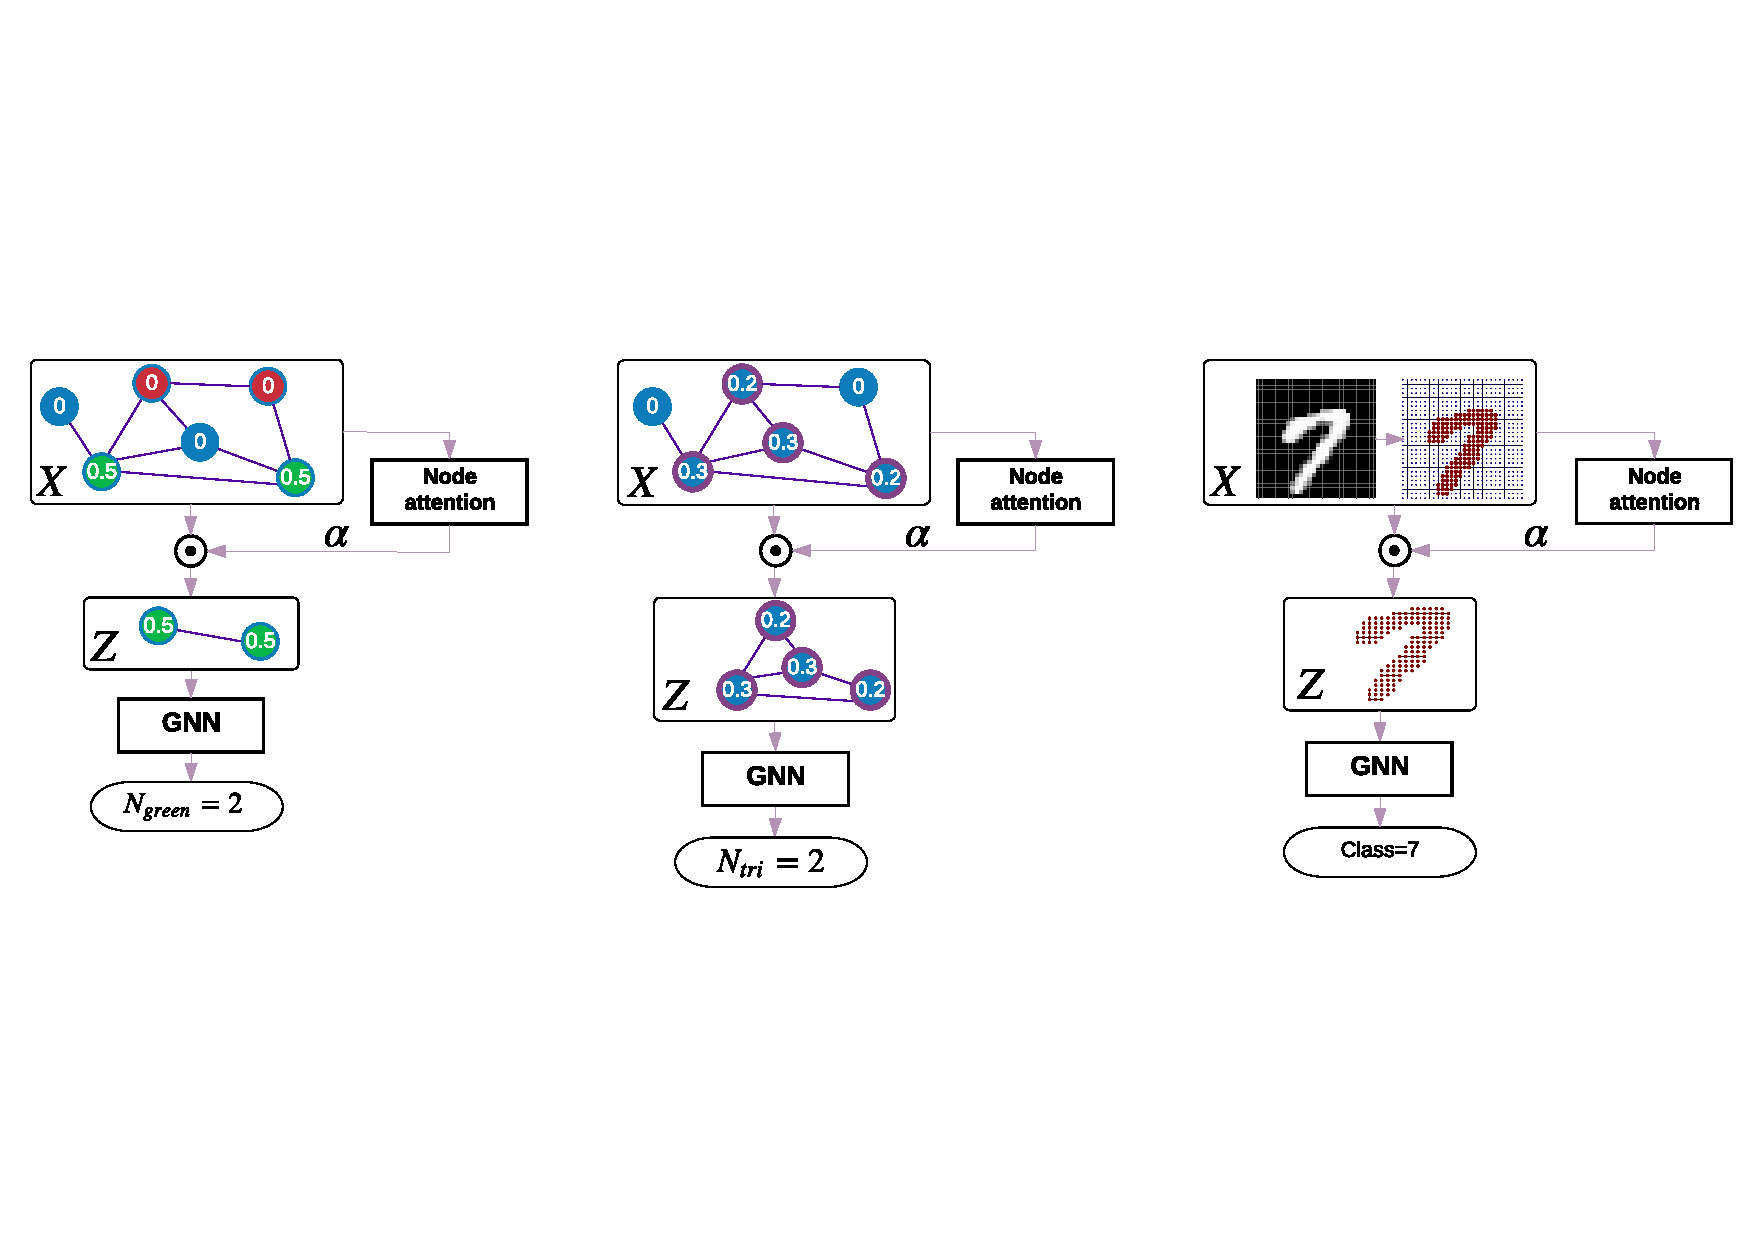
\includegraphics[width=0.27\textwidth, align=c, trim={10cm 6cm 10.8cm 6.1cm}, clip]{tasks}} &
			{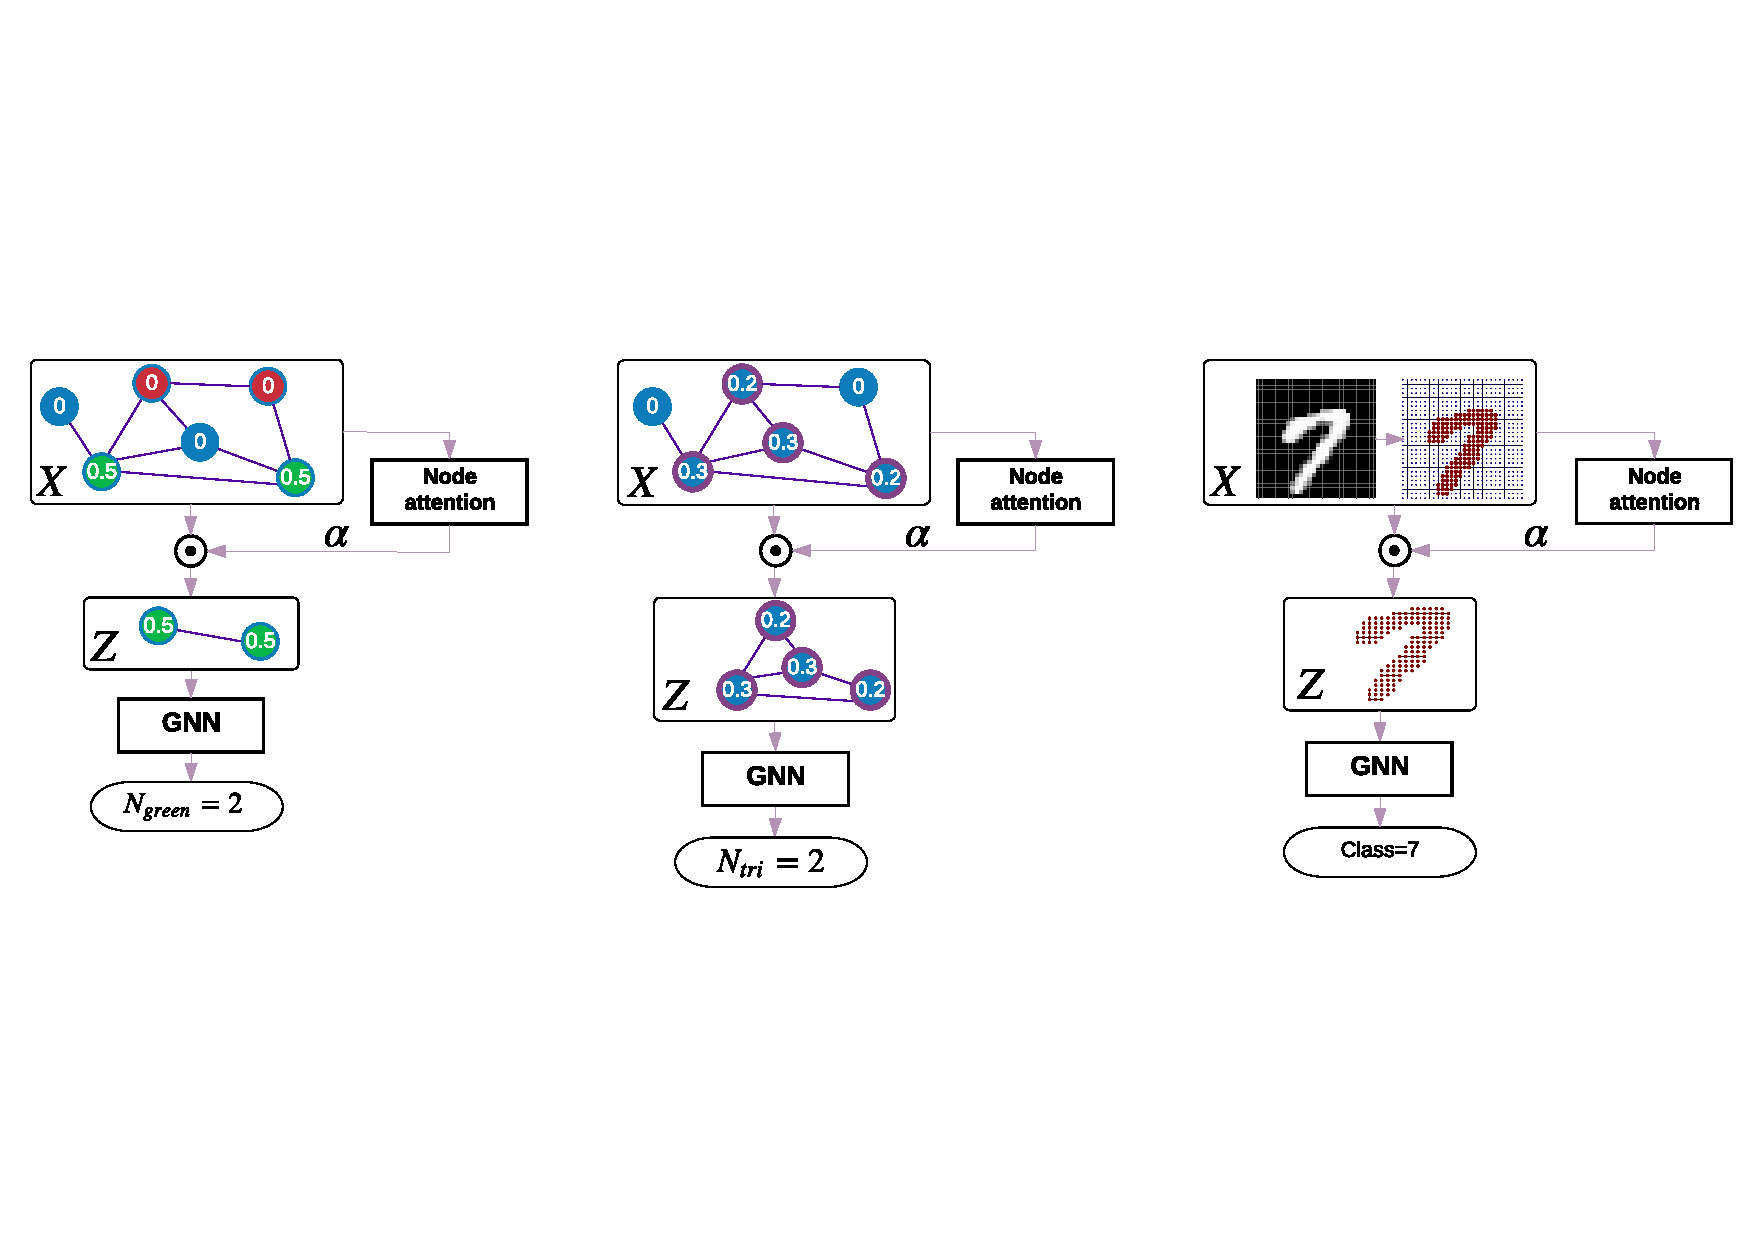
\includegraphics[width=0.3\textwidth, align=c, trim={20cm 6cm 0.3cm 6cm}, clip]{tasks}} \\
			(a) \textsc{Colors} & (b) \textsc{Triangles} & (c) \mnistfull \\
		\end{tabular}
	\end{center}
	\vspace{-10pt}
	\caption{\small Three tasks with a controlled environment we consider in this work. The values inside the nodes are ground truth attention coefficients, $\mathbf{\alpha}_i^{GT}$, which we find heuristically (see \secref{\ref{sec:datasets}}).}
	\label{fig:tasks}
\end{figure}
%
Despite the appealing nature of attention, it is often unstable to train and the conditions under which it fails or succeeds are unclear.
Motivated by insights of~\citep{xu2018powerful} recently proposed Graph Isomorphism Networks (GIN), we design two simple graph reasoning tasks
that allow us to study attention in a controlled environment where we know ground truth attention.
The first task is counting colors in a graph (\textsc{Colors}), where a color is a unique discrete feature. The second task is counting the number of triangles in a graph (\textsc{Triangles}). We confirm our observations on a standard benchmark, \mnistfull~\citep{lecun1998gradient} (\fig{\ref{fig:tasks}}), and identify factors influencing the effectiveness of attention.

Our synthetic experiments also allow us to study the ability of attention \gnns to generalize to larger, more complex or noisy graphs. Aiming to provide a recipe to train more effective, stable and robust attention \gnns, we propose a \wsup~scheme to train attention, that does not require ground truth attention scores, and as such is agnostic to a dataset and the choice of a model.
We validate the effectiveness of this scheme on our synthetic datasets, as well as on \mnistfull~and on real graph classification benchmarks in which ground truth attention is unavailable and hard to define, namely \collab~\citep{leskovec2007graph, shrivastava2014new}, \proteins~\citep{borgwardt2005protein}, and \dd~\citep{dobson2003distinguishing}.

\section{Model}

We study two variants of \gnns: Graph Convolutional Networks (GCN)~\citep{kipf2016semi} and Graph Isomorphism Networks (GIN)~\citep{xu2018powerful}. One of the main ideas of GIN is to replace the \textsc{Mean} aggregator over nodes, such as the one in GCN, with a \textsc{Sum} aggregator, and add more fully-connected layers after aggregating neigboring node features. The resulting model can distinguish a wider range of graph structures than previous models~\cite[Figure 3]{xu2018powerful}.

\subsection{Thresholding by attention coefficients}
To pool the nodes in a graph using the method from\citep{graphunet2018} a predefined ratio $r=|P| / N$ must be chosen for the entire dataset \eqref{eq:top-k}. For instance, for $r=0.8$ only 80\% of nodes are left after each pooling layer. Intuitively, it is clear that this ratio should be different for small and large graphs.
Therefore, we propose to choose threshold $\tilde{\mathbf{\alpha}}$, such that only nodes with attention values $\mathbf{\alpha}_i > \tilde{\mathbf{\alpha}}$ are propagated:
%
\begin{equation}
\label{eq:top-k_ours}
%\Z_i = \mathbf{\alpha}_i \X_i, \forall\ i: \mathbf{\alpha}_i > \tilde{\mathbf{\alpha}}.
\Z_i =
\begin{cases}
\mathbf{\alpha}_i \X_i,& \forall i: \mathbf{\alpha}_i > \tilde{\mathbf{\alpha}} \\
\emptyset, & \text{otherwise}.
\end{cases}
\end{equation}
%
Note, that dropping nodes from a graph is different from keeping nodes with very small, or even zero, feature values, because a bias is added to node features after the following graph convolution layer affecting features of neighbors. An important potential issue of dropping nodes is the change of graph structure and emergence of isolated nodes. However, in our experiments we typically observe that the model predicts similar $\mathbf{\alpha}$ for nearby nodes, so that an entire local neighborhood is pooled or dropped, as opposed to clustering-based methods which collapse each neighborhood to a single node. We provide a quantitative and qualitative comparison in \secref{\ref{sec:exper}}.

\subsection{Attention subnetwork}
To train an attention model that predicts the coefficients for nodes, we consider two approaches: (1)~Linear Projection~\citep{graphunet2018}, where a single layer projection $\mathbf{p} \in \mathbb{R}^C$ is trained: $\mathbf{\alpha}_{pre} = \X \mathbf{p}$; and (2)~DiffPool~\citep{ying2018hierarchical}, where a separate \gnn is trained:
%
\begin{equation}
\label{eq:attn_gcn}
\mathbf{\alpha}_{pre} = \text{GNN}(\A, \X),
\end{equation}
%
where $\A$ is the adjacency matrix of a graph.
In all cases, we use a softmax activation~\citep{vaswani2017attention,park2016attentive} instead of tanh in~\citep{graphunet2018}, because it provides more interpretable results  and ecourages sparse outputs: $\mathbf{\alpha} = \text{softmax}(\mathbf{\alpha}_{pre})$.
To train attention in a supervised or \wsup~way, we use the Kullback-Leibler divergence loss (see \secref{\ref{sec:arch_train}}).

Note that the GNN used in \eqref{eq:attn_gcn} is called an attention subnetwork because its outputs $\mathbf{\alpha} = \text{softmax}(\mathbf{\alpha}_{pre})$ are used to weight the input node features $\X$ according to \eqref{eq:top-k_ours}: $\Z = \mathbf{\alpha} \odot \X$. This way $\mathbf{\alpha}$ defines how much the following layers pay attention (or attend) to each of the nodes as we discuss in \secref{\ref{sec:attn_intro}}.

\subsection{ChebyGIN}

In some of our experiments, the performance of both GCNs and GINs is quite poor and, consequently, it is also hard for the attention subnetwork to learn. By combining GIN~\citep{xu2018powerful} with ChebyNet~\citep{defferrard2016convolutional}, we propose a stronger model, ChebyGIN.
ChebyNet is a multiscale extension of GCN~\citep{kipf2016semi}, so that for the first scale, $k=0$, node features are node features themselves, for $k=1$ features are averaged over one-hop neighbors, for $k=2$ - over two-hop neighbors and so forth (see \eqref{eq:cheb_graph_conv} in \S~\ref{sec:bg_gnn}).
To implement the \textsc{Sum} aggregator in ChebyGIN, we multiply node features $\X$ by a diagonal node degree matrix $\D_{ii}=\sum_j \A_{ij}$ starting from $k=1$. We also add more fully-connected layers (denoted as $\text{MLP}^{(l)}$) after feature aggregation as in GIN. Thus, following \eqref{eq:cheb_graph_conv}, the $l$-th layer of our ChebyGIN is defined as:
%
\begin{equation}
\label{eq:chebygin}
\X^{(l+1)} = \text{MLP}^{(l)} \Big(\sum^{K-1}_{k=0} \D_{ii}^{(k)} T_k(\tilde{\Lapl}) \X^{(l)} \W^{(l)}_k \Big),
\end{equation}
%
\noindent where $\D_{ii}^{(k)} = \mathbf{I}_N$ for $k=0$ and $\D_{ii}^{(k)} = \sum_j \A_{ij}$ for $k > 0$. $T_k(\tilde{\Lapl})$ are the Chebyshev polynomials applied to a rescaled graph Laplacian $\tilde{\Lapl}$; $\W^{(l)}_k$ are trainable weights. See a detailed description of these terms in \S~\ref{sec:bg_gnn} and the implementation details of ChebyGIN in our code \url{https://github.com/bknyaz/graph_attention_pool/blob/master/chebygin.py}.

\section{Experiments}
\label{sec:exper}
We introduce the color counting task (\textsc{Colors}) and the triangle counting task (\textsc{Triangles}) in which we generate synthetic training and test graphs. We also experiment with MNIST images~\citep{lecun1998gradient} and three molecule and social datasets. In \colors, \tri~and \mnistfull~tasks (\fig{\ref{fig:tasks}}), we assume to know ground truth attention, i.e. for each node~$i$ we heuristically define its importance in solving the task correctly, $\mathbf{\alpha}_i^{GT} \in [0,1]$, which is necessary to train (in the supervised case) and evaluate our attention models.


\subsection{Datasets}
\label{sec:datasets}
\densepar{\textsc{Colors}.} We introduce the color counting task. We generate random graphs where features for each node are assigned to one of the three one-hot values (colors): [1,0,0] (red), [0,1,0] (green), [0,0,1] (blue). The task is to count the number of green nodes, $N_{green}$. This is a trivial task, but it lets us study the influence of initialization of the attention model $\mathbf{p} \in \mathbb{R}^3$ on the training dynamics.
In this task, graph structure is unimportant and edges of graphs act like a medium to exchange node features. Ground truth attention is $\mathbf{\alpha}_i^{GT}=1 / N_{green}$, when $i$ corresponds to green nodes and $\mathbf{\alpha}_i^{GT}=0$ otherwise.
We also extend this dataset to higher $n$-dimensional cases $\mathbf{p} \in \mathbb{R}^n$ to study how model performance changes with $n$.
In these cases, node features are still one-hot vectors and we classify the number of nodes where the second feature is one.

\densepar{\textsc{Triangles}.} Counting the number of triangles in a graph is a well-known task which can be solved analytically by computing $\text{trace}(\A^3) / 6$, where $\A$ is an adjacency matrix. This task turned out to be hard for \gnns, so we add node degree features as one-hot vectors to all graphs, so that the model can exploit both graph structure and features. Compared to the \textsc{Colors} task, here it is more challenging to study the effect of initializing $\mathbf{p}$, but we can still calculate ground truth attention as $\mathbf{\alpha}_i^{GT}=T_i / \sum_i T_i$, where $T_i$ is the number of triangles that include node $i$, so that $\mathbf{\alpha}_i^{GT} = 0$ for nodes that are not part of triangles.

\densepar{\textsc{Mnist-75sp}.} \textsc{Mnist}~\citep{lecun1998gradient} contains 70k grayscale images of size 28$\times$28 pixels. While each of 784 pixels can be represented as a node, we follow~\citep{monti2017geometric, fey2018splinecnn} and consider an alternative approach to highlight the ability of \gnns to work on irregular grids. In particular, each image can be represented as a small set of superpixels without losing essential class-specific information (see \fig{\ref{fig:test_subsets}}). We compute SLIC~\citep{achanta2012slic} superpixels for each image and build a graph, in which each node corresponds to a superpixel with node features being pixel intensity values and coordinates of their centers of masses. We extract $N\leq75$ superpixels, hence the dataset is denoted as \mnist.
Edges are formed based on spatial distance between superpixel centers as in~\cite[Eq.~8]{defferrard2016convolutional}. Each image depicts a handwritten digit from 0 to 9 and the task is to classify the image. Ground truth attention is considered to be $\mathbf{\alpha}_i^{GT}=1 / N_{nonzero}$ for superpixels with nonzero intensity, and $N_{nonzero}$ is the total number of such superpixels. The idea is that only nonzero superpixels determine the digit class.\looseness-1

\densepar{Molecule and social datasets.}
\label{sec:graph_data}
We extend our study to more practical cases, where ground truth attention is not available, and experiment with protein datasets: \proteins~\citep{borgwardt2005protein} and \dd~\citep{dobson2003distinguishing}, and a scientific collaboration dataset, \collab~\citep{leskovec2007graph, shrivastava2014new}.
These are standard graph classification benchmarks.
A standard way to evaluate models on these datasets is to perform 10-fold cross-validation and report average accuracy~\citep{yanardag2015deep, ying2018hierarchical}.
In this work, we are concerned about a model's ability to generalize to larger and more complex or noisy graphs, therefore, we generate splits based on the number of nodes. For instance, for \proteins~we train on graphs with $ N \leq 25$ nodes and test on graphs with $ 6 \leq N \leq 620$ nodes (see Table~\ref{table:results_graphs} for details about splits of other datasets and results).\looseness-1

%A detailed description of tasks and model hyperparameters is provided in the \apdx.

%\vspace{-10pt}
\subsection{Generalization to larger and noisy graphs}
%\vspace{-10pt}
One of the core strengths of attention is that it makes it easier to generalize to unseen, potentially more complex and/or noisy, inputs by reducing them to better resemble certain inputs in the training set. To examine this phenomenon, for \textsc{Colors} and \textsc{Triangles} tasks we add test graphs that can be several times larger (\textsc{Test-Large}) than the training ones. For \textsc{Colors} we further extend it by adding unseen colors to the test set (\textsc{Test-LargeC}) in the format $[c_1, c_2, c_3, c_4]$, where $c_i=0$ for $i \neq 2$ if $c_2=1$ and $c_i \in [0,1]$ for $i \neq 2$ if $c_2=0$, i.e.~there is no new colors that have nonzero values in a green channel. This can be interpreted as adding mixtures of red, blue and transparency channels, with nine possible colors in total as opposed to three in the training set (\fig{\ref{fig:test_subsets}}).


\newcommand{\figwidth}{0.14\textwidth}
\newcommand{\rangeupper}[1]{\tiny{($N\leq#1$)}}
\newcommand{\rangetwo}[2]{\tiny{($#1<N\leq#2$)}}
\begin{figure}[h!]
    \newcommand{\figtasks}[2]{\includegraphics[width=\figwidth, align=c, trim=#1, clip]{#2}}
    \centering
	\begin{center}
		\scriptsize
		\setlength{\tabcolsep}{7pt}
		\begin{tabularx}{\textwidth}{ccccc}
			{\rotatebox[origin=c]{90}{\textsc{\textbf{Colors}} }} &
			\figtasks{{2cm 0.5cm 1.3cm 1.3cm}}{colors_train.pdf} &
			\figtasks{{2cm 0.5cm 1.3cm 1.3cm}}{colors_test1.pdf} &
			\figtasks{{2cm 0.5cm 1.3cm 1.3cm}}{colors_test2.pdf} &
			\figtasks{{2cm 0.5cm 1.3cm 1.3cm}}{colors_test_mix.pdf} \\
			& \textsc{Train} \rangeupper{25} & \textsc{Test-Orig} \rangeupper{25} & \textsc{Test-Large} \rangetwo{25}{200} & \textsc{Test-LargeC} \rangetwo{25}{200} \\
			\hline \\
		\end{tabularx}
		\setlength{\tabcolsep}{21pt}
		\begin{tabularx}{\textwidth}{cccc}
			\hspace{-25pt}
			\multirow{2}{*}{\rotatebox[origin=c]{90}{\parbox{0.8cm}{\textsc{\textbf{Triangles}}}}} &
			\figtasks{{1.5cm 0.7cm 0cm 0cm}}{triangles_train1.pdf} &
			\figtasks{{1.5cm 0.7cm 0cm 0cm}}{triangles_test1.pdf} &
			\figtasks{{1.5cm 0.7cm 0cm 0cm}}{triangles_test2.pdf} \\
			& \textsc{Train} \rangeupper{25} & \textsc{Test-Orig} \rangeupper{25} & \textsc{Test-Large} \rangetwo{25}{100}\\
			\hline \\
		\end{tabularx}
		\setlength{\tabcolsep}{12pt}
		\begin{tabularx}{\textwidth}{ccccc}
			\hspace{-7pt} \multirow{2}{*}{\rotatebox[origin=c]{90}{\parbox{0.9cm}{\mbox{\textbf{\mnist}}}}} &
			\figtasks{{0cm 0cm 0cm 0cm}}{7_train_75sp.pdf} &
			\figtasks{{0cm 0cm 0cm 0cm}}{7_test_75sp.pdf} &
			\figtasks{{0cm 0cm 0cm 0cm}}{7_noise0_4_test_75sp.pdf} &
			\figtasks{{0cm 0cm 0cm 0cm}}{7_colornoise0_6_test_75sp.pdf} \\
			& \textsc{Train}\tiny{($N=64$)} & \textsc{Test-Orig}\tiny{($N=63$)} & \textsc{Test-Noisy}\tiny{($N=63$)} & \textsc{Test-NoisyC}\tiny{($N=63$)} \\
		\end{tabularx}
	\end{center}
	\vspace{-10pt}
	\caption{\small Examples from training and test sets. For \colors, the correct label is $N_{green}=4$ in all cases; for \tri~$N_{tri}=3$ and color intensities denote ground truth attention values $\mathbf{\alpha}^{GT}$. The range of the number of nodes, $N$, is shown in each case. For \mnist, we visualize graphs for digit 7 by assigning an average intensity value to all pixels within a superpixel. Even though superpixels have certain shapes and borders between each other (visible only on noisy graphs), we feed only superpixel intensities and coordinates of their centers of masses to our \gnns.}
	\label{fig:test_subsets}
	\vspace{-8pt}
\end{figure}

Neural networks (NNs) have been observed to be brittle if they are fed with test samples corrupted in a subtle way, i.e.~by adding a noise~\citep{dodge2017study} or changing a sample in an adversarial way~\citep{szegedy2013intriguing}, such that a human can still recognize them fairly well. To study this problem, test sets of standard image benchmarks have been enlarged by adding corrupted images~\citep{hendrycks2019benchmarking}.

Graph neural networks, as a particular case of NNs, inherit this weakness. The attention mechanism, if designed and trained properly, can improve a net's robustness by attending to only important and ignoring misleading parts (nodes) of data. In this work, we explore the ability of \gnns with and without attention to generalize to noisy graphs and unseen node features. This should help us to understand the limits of \gnns, and potentially NNs in general, with attention and conditions when it succeedes and when it does not. To this end, we generate two additional test sets for \mnist. In the first set, \textsc{Test-Noisy}, we add Gaussian noise, drawn from $\mathcal{N}(0, 0.4)$, to superpixel intensity features, i.e.~the shape and coordinates of superpixels are the same as in the original clean test set. In the second set, \textsc{Test-Noisy-C}, we colorize images by adding two more channels and add independent Gaussian noise, drawn from $ \mathcal{N}(0, 0.6)$, to each channel (\fig{\ref{fig:test_subsets}}).

\subsection{Network architectures and training}
\label{sec:arch_train}
We build 2 layer \gnns for \textsc{Colors} and 3 layer \gnns for other tasks with 64 filters in each layer, except for \mnist~where we have more filters. Our baselines are \gnns with global sum or max pooling (gpool), DiffPool~\citep{ying2018hierarchical} and top-k pooling~\citep{graphunet2018}. We add two layers of our pooling for \tri, each of which is a \gnn with 3 layers and 32 filters \eqref{eq:attn_gcn}; whereas a single pooling layer in the form of vector $\mathbf{p}$ is used in other cases.
We train all models with Adam~\citep{kingma2014adam}, learning rate 1e-3, batch size 32, weight decay 1e-4.

For \textsc{Colors} and \textsc{Triangles} we minimize the regression loss (MSE) and cross entropy (CE) for other tasks, denoted as $\mathcal{L}_{MSE/CE}$. For experiments with supervised and \wsup~(described below in \secref{\ref{sec:wsup}}) attention, we additionally minimize the Kullback-Leibler (KL) divergence loss between ground truth attention $\mathbf{\alpha}^{GT}$ and predicted coefficients $\mathbf{\alpha}$. The KL term is weighted by scale $\beta$, so that the total loss for some training graph with $N$ nodes becomes:
%
\begin{equation}
\label{eq:kl_div_loss}
\mathcal{L} = \mathcal{L}_{MSE/CE} + \frac{\beta}{N}\sum_i \mathbf{\alpha}_i^{GT} \text{log}(\frac{\mathbf{\alpha}_i^{GT}}{\mathbf{\alpha}_i}).
\end{equation}
%
%where $\beta$ controls the scale and importance of the KL term.
%
We repeat experiments at least 10 times and report an average accuracy and standard deviation in Tables~\ref{table:results} and~\ref{table:results_graphs}.
For \colors~we run experiments 100 times, since we observe larger variance.
In Table~\ref{table:results} we report results on all test subsets independently.
In all other experiments on \synthetic, we report an average accuracy on the combined test set.
For \real, we run experiments 10 times using splits described in \secref{\ref{sec:graph_data}}.

The only hyperparameters that we tune in our experiments are threshold $\tilde{\mathbf{\alpha}}$ in our method \eqref{eq:top-k_ours}, ratio $r$ in top-k \eqref{eq:top-k} and $\beta$ in \eqref{eq:kl_div_loss}. For synthetic datasets, we tune them on a validation set generated in the same way as \textsc{Test-Orig}. For \mnist, we use part of the training set. For \real, we tune them using 10-fold cross-validation on the training set.


\densepar{Attention correctness.} We evaluate attention correctness using area under the ROC curve (AUC) as an alternative to other methods, such as~\citep{liu2017attention}, which can be overoptimistic in some extreme cases, such as when all attention is concentrated in a single node or attention is uniformly spread over all nodes. AUC allows us to evaluate the ranking of $\mathbf{\alpha}$ instead of their absolute values. Compared to ranking metrics, such as rank correlation, AUC enables us to directly choose a pooling threshold $\tilde{\mathbf{\alpha}}$ from the ROC curve by finding a desired balance between false-positives (pooling unimportant nodes) and false-negatives (dropping important nodes).

To evaluate attention correctness of models with global pooling, we follow the idea from convolutional neural networks~\citep{zeiler2014visualizing}. After training a model, we remove node $i \in [1, N]$ and compute an absolute difference from prediction $y$ for the original graph:
%
\begin{equation}
\label{eq:heat_maps}
\mathbf{\alpha}_i^{WS} = \frac{|y_i - y|}{\sum_{j=1}^N |y_j - y|},
\end{equation}
%
where $y_i$ is a model's prediction for the graph without node $i$.
While this method shows surprisingly high AUC in some tasks, it is not built-in in training and thus does not help to train a better model and only implicitly interprets a model's prediction (Figures~\ref{fig:attn_mnist} and~\ref{fig:attn_graphs}). However, these results inspired us to design a \wsup~method described below.

\subsection{Weakly-supervised attention supervision}
\label{sec:wsup}
Although for \colors, \tri~and \mnist~we can define ground truth attention, so that it does not require manual labeling, in practice it is usually not the case and such annotations are hard to define and expensive, or even unclear how to produce. Based on results in Table~\ref{table:results}, supervision of attention is necessary to reveal its power. Therefore, we propose a weakly-supervised approach, agnostic to the choice of a dataset and model, that does not require ground truth attention labels, but can improve a model's ability to generalize.
Our approach is based on generating attention coefficients $\mathbf{\alpha}_i^{WS}$ \eqref{eq:heat_maps} and using them as labels to train our attention model with the loss defined in Eq~\ref{eq:kl_div_loss}.
We apply this approach to \colors, \tri~and \mnist~and observe peformance and robustness close to supervised models. We also apply it to \collab, \proteins~and \dd, and in all cases we are able to improve results compared to unsupervised attention.

\textbf{Training weakly-supervised models.}
Assume we want to train model \textbf{A} with ``weak-sup'' attention on a dataset without ground truth attention. We first need to train model \textbf{B} that has the same architecture as \textbf{A}, but does not have any attention/pooling between graph convolution layers. So, model \textbf{B} has only global pooling. After training \textbf{B} with the $\mathcal{L}_{MSE/CE}$ loss, we need to evaluate training graphs on \textbf{B} in the same way as during computation of $\mathbf{\alpha}^{WS}$ in \eqref{eq:heat_maps}. In particular, for each training graph $\cal G$ with $N$ nodes, we first make a prediction $y$ for the entire $\cal G$. Then, for each $i \in [1,N]$, we remove node $i$ from $\cal G$, and feed this reduced graph with $N-1$ nodes to model \textbf{B} recording the model's prediction $y_i$. We then use \eqref{eq:heat_maps} to compute $\mathbf{\alpha}^{WS}$ based on $y$ and $y_i$. Now, we can train \textbf{A} and use $\mathbf{\alpha}^{WS}$ instead of ground truth $\mathbf{\alpha}^{GT}$ in \eqref{eq:kl_div_loss} to optimize both \textit{MSE/CE} and \textit{KL} losses.\looseness-1

%\definecolor{extreme}{gray}{0.85}
%\definecolor{bad}{gray}{0.95}


\begin{table}[b!]
	%\newcommand\crule[3][black]{\textcolor{#1}{\rule{#2}{#3}}}
	%\vspace{-8pt}
	\caption{\small \textbf{Results on three tasks for different test subsets.} $\pm$ denotes standard deviation, not shown in case of small values (large values are explained in \secref{\ref{sec:results}}). \textsc{Attn} denotes attention accuracy in terms of AUC and is computed for the combined test set. The best result in each column (ignoring upper bound results) is bolded.
	\crule[bad]{12pt}{8pt} denotes poor results with relatively low accuracy and/or high variance;
	\crule[extreme]{12pt}{8pt} denotes failed cases with accuracy close to random and/or extremely high variance. $^\dagger$~For \colors~and \mnist, ChebyNets are used instead of ChebyGINs.\looseness-1}
    \vspace{-10pt}
	\scriptsize
	\label{table:results}
	\begin{center}
		\setlength{\tabcolsep}{2pt}
		\begin{tabular}{clllll|lll|llll}
			\toprule
			&  &\multicolumn{4}{c|}{\bf \colors} & \multicolumn{3}{c|}{\bf \tri}  & \multicolumn{4}{c}{\bf \mnist}\Tstrut\\
			& & \textsc{Orig} & \textsc{Large} & \textsc{LargeC} & \textsc{Attn} & \textsc{Orig} & \textsc{Large} & \textsc{Attn} & \textsc{Orig} & \textsc{Noisy} & \textsc{NoisyC} & \textsc{Attn} \\
			\midrule\\
			\multirow{3}{*}{\rotatebox[origin=c]{90}{\parbox{0.6cm}{\tiny \centering Global pool}}}
			& GCN & 97 & \cellcolor{bad}72\std{15} & \cellcolor{extreme}20\std{3} & 99.6 & 46\std{1} & \cellcolor{extreme}23\std{1}  & 79 & \cellcolor{bad}78.3\std{2} & \cellcolor{extreme}38\std{4} & \cellcolor{extreme}36\std{4} & 72\std{2}\\
			& GIN & \cellcolor{bad}96\std{10} & \cellcolor{bad}71\std{22} & \cellcolor{extreme}26\std{11} & 99.2 & 50\std{1} & \cellcolor{extreme}22\std{1} & 77 & 87.6\std{3} & \cellcolor{extreme}55\std{11} & \cellcolor{extreme}51\std{12} & 71\std{5} \\
			& ChebyGIN$^\dagger$ & \textbf{100} & \cellcolor{bad}93\std{12} & \cellcolor{extreme}15\std{7} & 99.8 & 66\std{1} & \cellcolor{bad}30\std{1} & 79 & \textbf{97.4} & \cellcolor{bad}80\std{12} & \cellcolor{bad}79\std{11} & 72\std{3} \\
			\hline \\
			\multirow{4}{*}{\rotatebox[origin=c]{90}{\parbox{1cm}{\tiny \centering Unsuperv.}}} &
			GIN, top-k & 99.6 & \cellcolor{extreme}17\std{4} & \cellcolor{extreme}9\std{3}  & 75\std{6} & 47\std{2} & \cellcolor{extreme}18\std{1} & 63\std{5} & 86\std{6} & \cellcolor{extreme}59\std{26} & \cellcolor{extreme}55\std{23} & \cellcolor{extreme}65\std{34} \\
			& GIN, ours & \cellcolor{bad}94\std{18} & \cellcolor{extreme}13\std{7} & \cellcolor{extreme}11\std{6} & \cellcolor{bad}72\std{15} & 47\std{3} & \cellcolor{extreme}20\std{2} & 68\std{3} & 82.6\std{8} & \cellcolor{extreme}51\std{28} & \cellcolor{extreme}47\std{24} & \cellcolor{extreme}58\std{31} \\
			& ChebyGIN$^\dagger$, top-k & \textbf{100} & \cellcolor{extreme}11\std{7} & \cellcolor{extreme}6\std{6} & \cellcolor{bad}79\std{20} & 64\std{5} & \cellcolor{extreme}25\std{2} & 76\std{6} & 92.9\std{4} & \cellcolor{extreme}68\std{26} & \cellcolor{extreme}67\std{25} & \cellcolor{extreme}52\std{37} \\
			& ChebyGIN$^\dagger$, ours & \cellcolor{extreme}80\std{30} & \cellcolor{extreme}16\std{10} & \cellcolor{extreme}11\std{6} & \cellcolor{bad}67\std{31} & 67\std{3} & \cellcolor{extreme}26\std{2} & 77\std{4} & 94.6\std{3} & \cellcolor{bad}80\std{23} & \cellcolor{bad}77\std{22} & \cellcolor{bad}78\std{31} \\
			\hline \\
			\multirow{4}{*}{\rotatebox[origin=c]{90}{\parbox{1cm}{\tiny Supervised}}}
			& GIN, topk & \cellcolor{bad}87\std{1} & \cellcolor{extreme}39\std{18} & \cellcolor{extreme}28\std{8} & \textbf{99.9} & 49\std{1} & \cellcolor{extreme}20\std{1} & 88 & 90.5\std{1} & 85.5\std{2} & \cellcolor{bad}79\std{5} & 99.3 \\
			& GIN, ours  & \textbf{100} & \textbf{96\std{9}} & \cellcolor{bad}\textbf{89\std{18}} & 99.8 & 49\std{1} & \cellcolor{extreme}22\std{1} & 76\std{1} & 90.9\std{0.4} & 85.0\std{1} & \cellcolor{bad}80\std{3} & 99.3 \\
			& ChebyGIN$^\dagger$, topk & \textbf{100} & \cellcolor{bad}86\std{15} & \cellcolor{extreme}31\std{15} & 99.8 & 83\std{1} & \cellcolor{bad}39\std{1} & \textbf{97} & 95.1\std{{0.3}} & 90.6\std{0.8} & \cellcolor{bad}83\std{16} & \textbf{100}  \\
			& ChebyGIN$^\dagger$, ours & \textbf{100} & 94\std{8} & \cellcolor{bad}75\std{17} & 99.8 & \textbf{88\std{1}} & \textbf{48\std{1}} & 96 & 95.4\std{0.2} & \textbf{92.3\std{0.4}} & \cellcolor{bad}\textbf{86\std{16}} & \textbf{100} \Bstrut \\
			\hline \Tstrut \\
			\multirow{1}{*}{\rotatebox[origin=c]{90}{\parbox{0.15cm}{\tiny \centering Weak sup.}}} &
			ChebyGIN$^\dagger$, ours & \textbf{100} &  90\std{6} & \cellcolor{bad}73\std{14} & \textbf{99.9} & 68\std{1} & \cellcolor{bad}30\std{1} & 88 & 95.8\std{0.4} & 88.8\std{4} & \textbf{86\std{9}} & 96.5\std{1} \Tstrut \Bstrut\\
			\hline
			\hline \\
			\multirow{2}{*}{\rotatebox[origin=c]{90}{\parbox{0.5cm}{\tiny \centering Upper bound}}}
			& GIN & 100 & 100 & 100 & 100 & 94\std{1} & 85\std{2} & 100 & 93.6\std{0.4} & 90.8\std{1} & 90.8\std{1} & 100 \\
			& ChebyGIN$^\dagger$ & 100 & 100 & 100 & 100 & 99.8 & 99.4\std{1} & 100 & 96.9\std{0.1} & 94.8\std{0.3} & 95.1\std{0.3} & 100 \\
			\bottomrule
			\vspace{-15pt}
		\end{tabular}
	\end{center}
\end{table}


\begin{figure}%[]
	\begin{center}
		\small
		\setlength{\tabcolsep}{1.5pt}
		\begin{tabular}{cccc}
			\begin{tikzpicture}
			\node[anchor=south west,inner sep=0] (image) at (0,0) {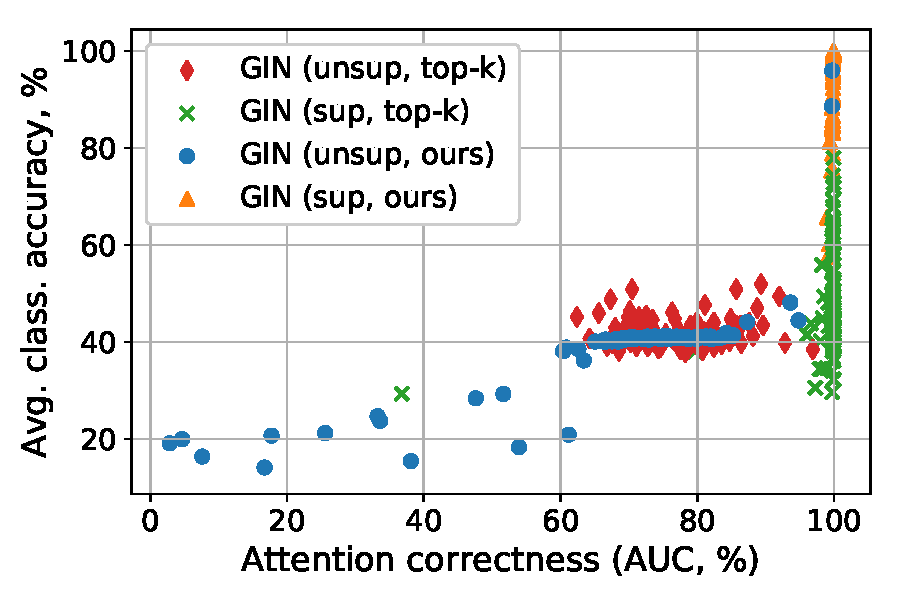
\includegraphics[width=0.24\textwidth, trim={0.3cm 0.4cm 0.3cm 0.3cm}, clip]{fig3/colors_gin_sup_ada_top_Acc_vs_AUC_dim3}};
			\begin{scope}[x={(image.south east)},y={(image.north west)}]
			\draw[green,thick,dashed,dash pattern=on 3pt off 2pt] (0.88,0.25) rectangle (0.97,0.98);
			\end{scope}
			\end{tikzpicture}
			&
			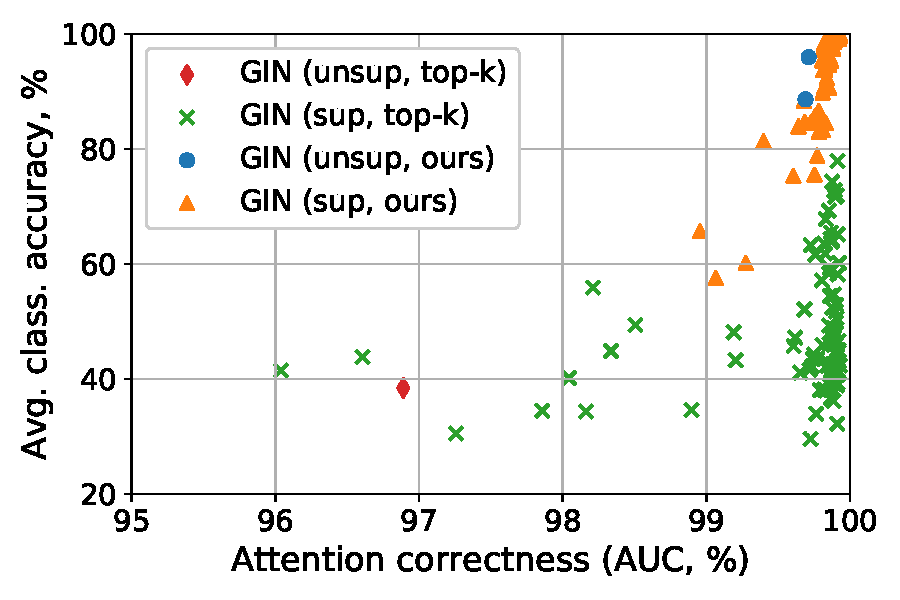
\includegraphics[width=0.24\textwidth, trim={0.3cm 0.4cm 0.3cm 0.3cm}, clip]{fig3/colors_gin_sup_ada_top_Acc_vs_AUC_zoomed_dim3} &

			\begin{tikzpicture}
			\node[anchor=south west,inner sep=0] (image) at (0,0) {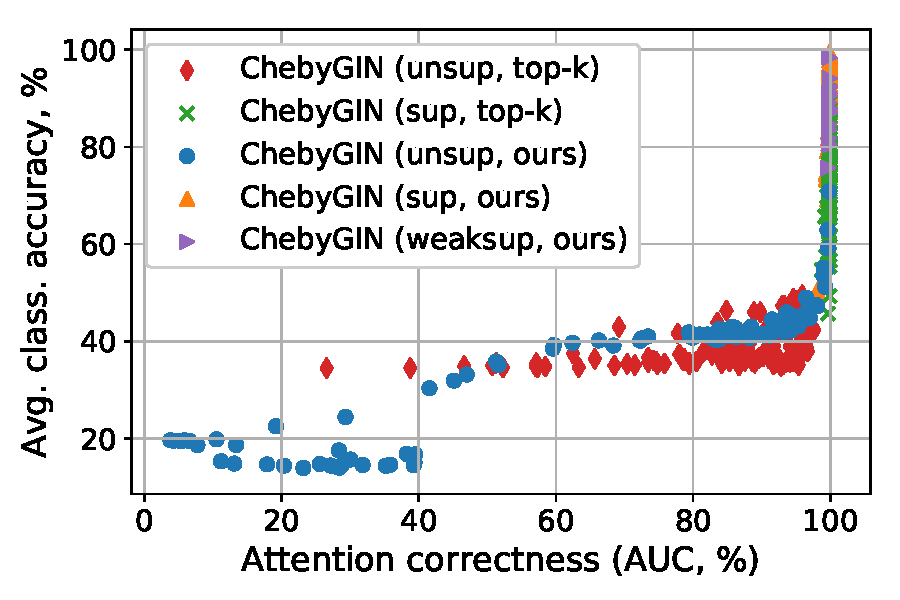
\includegraphics[width=0.24\textwidth, trim={0.3cm 0.4cm 0.3cm 0.3cm}, clip]{fig3/colors_cheb_sup_ada_top_Acc_vs_AUC_dim3}};
			\begin{scope}[x={(image.south east)},y={(image.north west)}]
			\draw[green,thick,dashed,dash pattern=on 3pt off 2pt] (0.88,0.25) rectangle (0.97,0.98);
			\end{scope}
			\end{tikzpicture}
			&
			{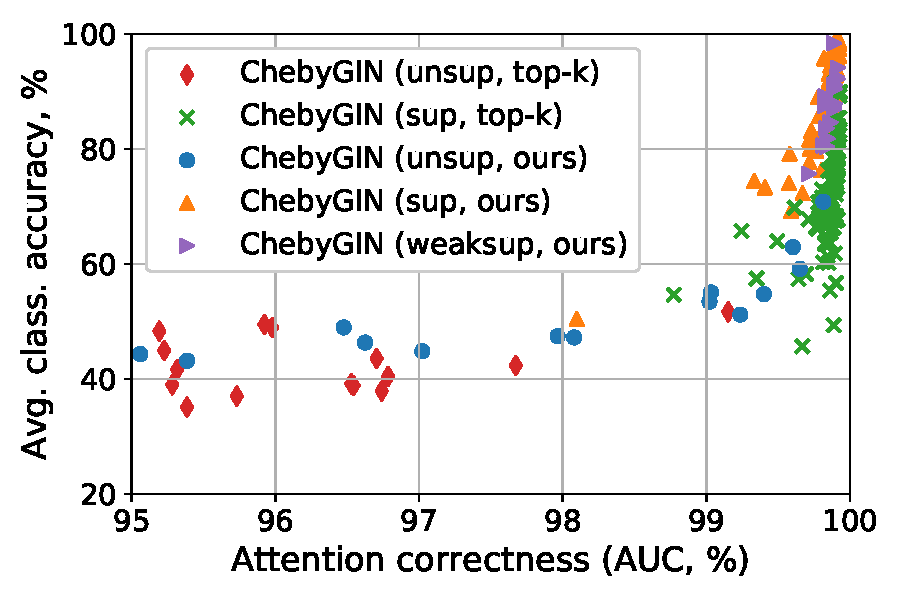
\includegraphics[width=0.24\textwidth, trim={0.3cm 0.4cm 0.3cm 0.3cm}, clip]{fig3/colors_cheb_sup_ada_top_Acc_vs_AUC_zoomed_dim3}} \\
			(a) & (a)-zoomed & (b) & (b)-zoomed \\

			{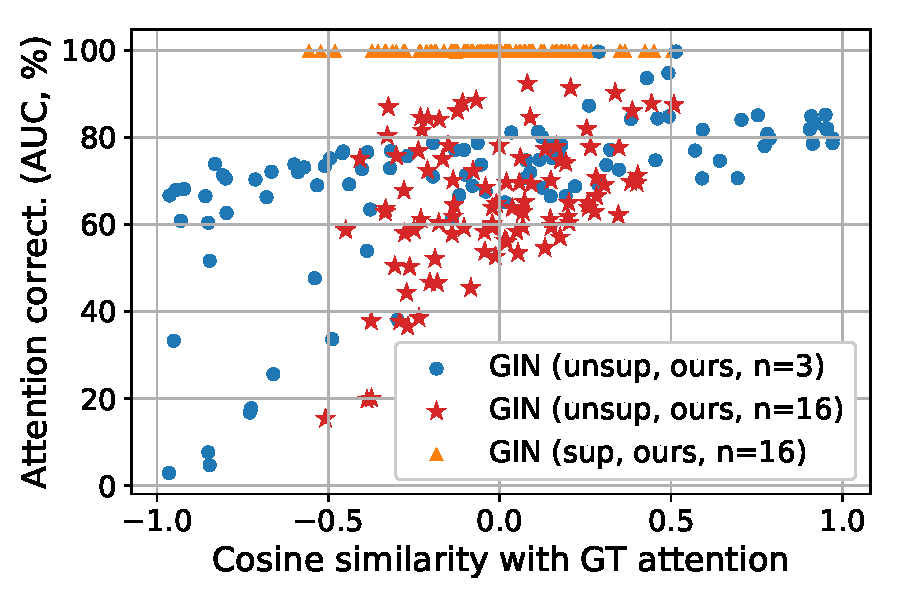
\includegraphics[width=0.24\textwidth, align=c, trim={0.3cm 0.4cm 0.3cm 0.3cm}, clip]{fig3/GIN_AUC_vs_Cos_dim3_16}} &
			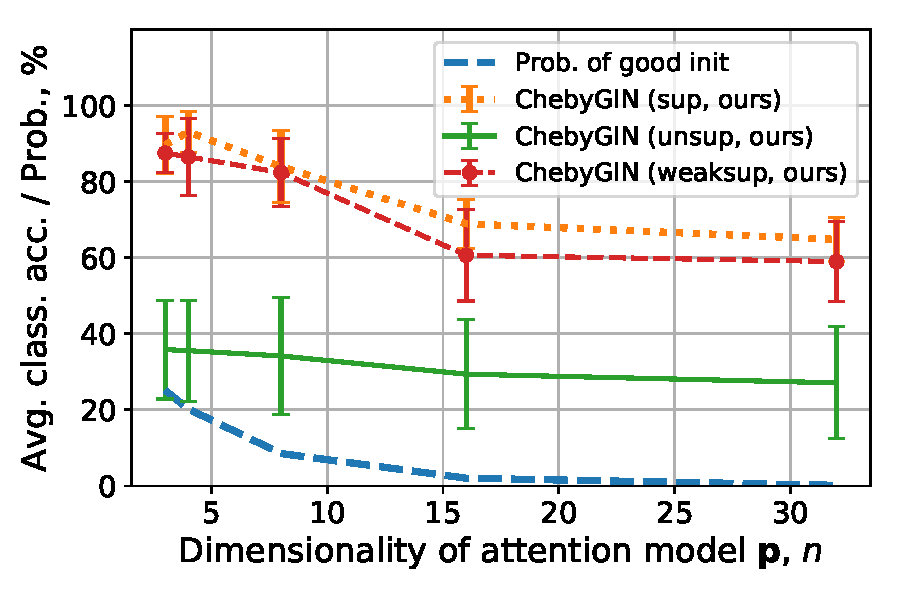
\includegraphics[width=0.24\textwidth, align=c, trim={0.3cm 0.4cm 0.3cm 0.3cm}, clip]{fig3/Cheb_ACC_vs_Dim} &

			{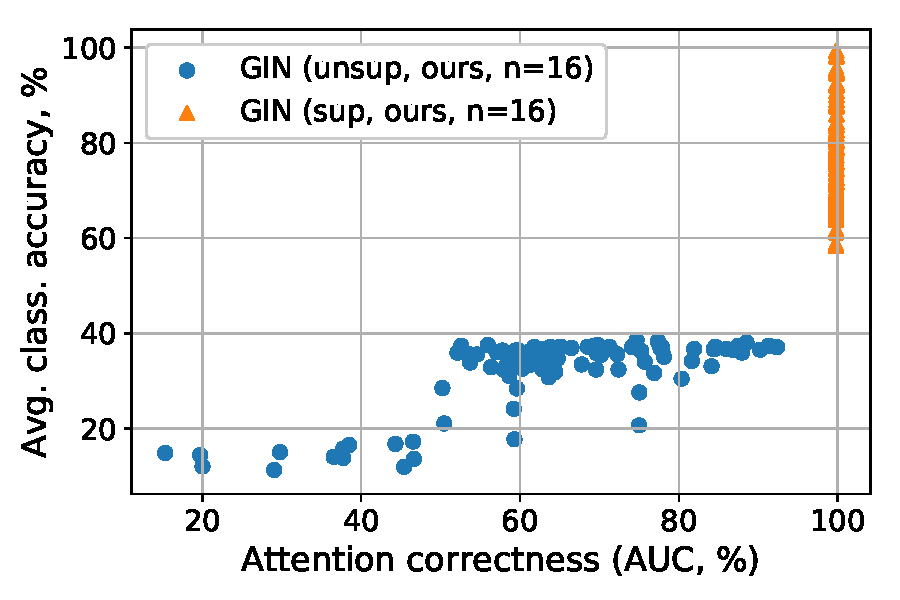
\includegraphics[width=0.24\textwidth, align=c, trim={0.3cm 0.4cm 0.3cm 0cm}, clip]{fig3/colors_gin_sup_ada_top_Acc_vs_AUC_dim16}} &
			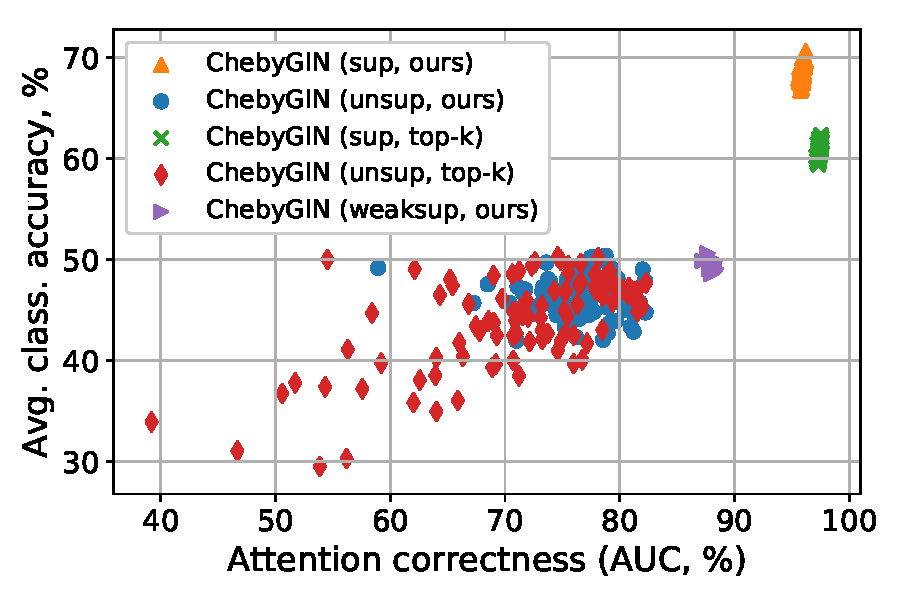
\includegraphics[width=0.24\textwidth, align=c, trim={0.3cm 0.4cm 0.3cm 0cm}, clip]{fig3/triangles_cheb_ACC_vs_Acc} \\
			(c) & (d) & (e)  & (f)
		\end{tabular}
	\end{center}
	\vspace{-18pt}
	\caption{\small Disentangling factors influencing attention and classification accuracy for \textsc{Colors} \textit{(a-e)} and \textsc{Triangles} \textit{(f)}. Accuracies are computed over all test subsets. Notice the exponential growth of classification accuracy depending on attention correctness \textit{(a,b)}, see zoomed plots \textit{(a)}-zoomed, \textit{(b)}-zoomed for cases when attention AUC$>$95\%. \textit{(d)} Probability of a good initialization is estimated as the proportion of cases when cosine similarity $>$ 0.5; error bars indicate standard deviation. \textit{(c-e)} show results using a higher dimensional attention model, $\mathbf{p} \in \mathbb{R}^n$.}
	%\vspace{-10pt}
	\label{fig:accuracy_cos_sim}
\end{figure}

\section{Analysis of results}
\label{sec:results}
In this work, we aim to better understand attention and generalization in graph neural networks, and,  based on our empirical findings, below we provide our analysis for the following questions.

\densepar{How powerful is attention over nodes in \gnns?}
Our results on the \synthetic~datasets suggest that the main strength of attention over nodes in \gnns is the ability to generalize to more complex or noisy graphs at test time. This ability essentially transforms a model that fails to generalize into a fairly robust one. Indeed, a classification accuracy gap for \textsc{Colors-LargeC} between the best model without supervised attention (GIN with global pooling) and a similar model with supervised attention (GIN, sup) is more than 60\%. For \textsc{Triangles-Large} this gap is 18\%  and for \textsc{MNIST-75sp-Noisy} it is more than 12\%. This gap is even larger if compared to upper bound cases indicating that our supervised models can be further tuned and improved. Models with supervised or \wsup~attention also have a more narrow spread of results (\fig{\ref{fig:accuracy_cos_sim}}).



\begin{figure}[thb]
	\newcommand{\width}{0.28\textwidth}
	\begin{center}
		\begin{small}
			\setlength{\tabcolsep}{3pt}
			\begin{tabular}{cccc}
				\multicolumn{4}{c}{
					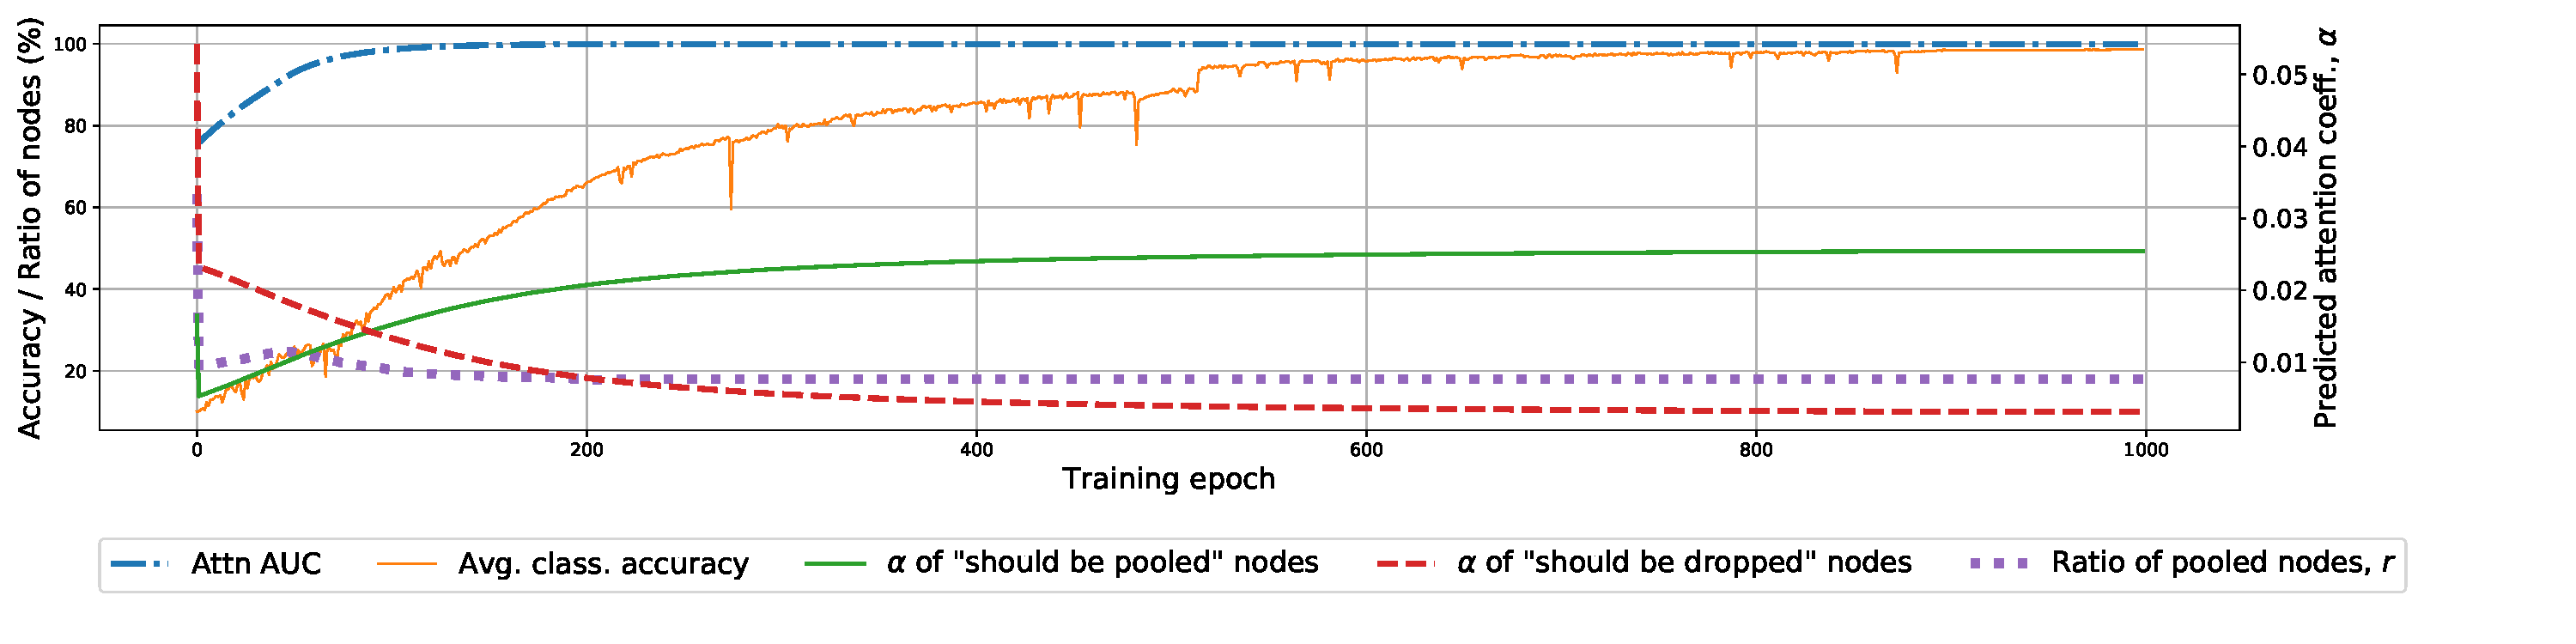
\includegraphics[width=0.95\textwidth, trim={1.5cm 1cm 3cm 10.5cm}, clip]{colors_init/legend.pdf}} \\
				& \scriptsize bad initialization (cos.~sim.=-0.75) &\scriptsize
				good initialization (cos.~sim.=0.75) &
				\scriptsize optimal initialization (cos.~sim.=1.00) \\
				\rotatebox[origin=c]{90}{\small \textsc{Unsupervised}} &
				{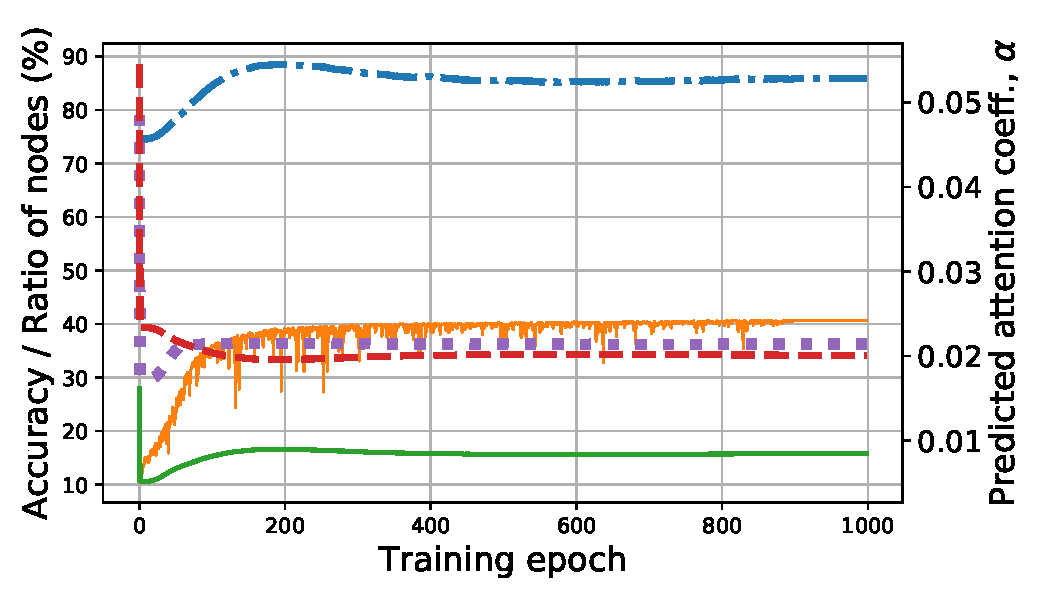
\includegraphics[width=\width, align=c, trim={0cm 0cm 0.5cm 0cm}, clip]{colors_init/bad_unsup}} & %\hspace{0.5cm}
				{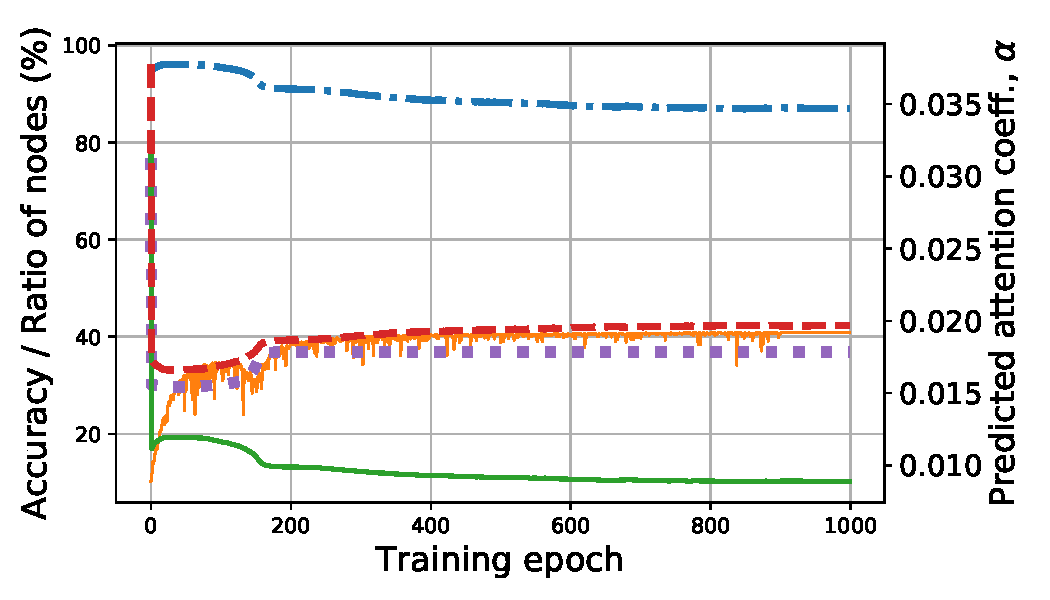
\includegraphics[width=\width, align=c, trim={0cm 0cm 0.5cm 0cm}, clip]{colors_init/good1_unsup}} &
				{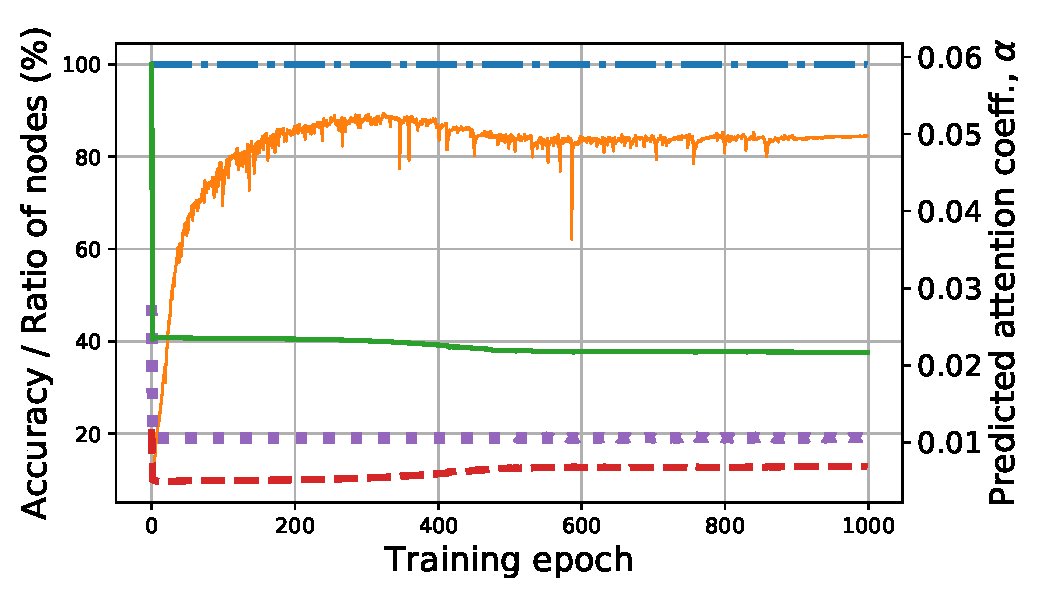
\includegraphics[width=\width, align=c, trim={0cm 0cm 0.5cm 0cm}, clip]{colors_init/optimal4_unsup}} \\
				& (a) & (b) & (c) \\
				\rotatebox[origin=c]{90}{\small \textsc{Supervised}} &
				{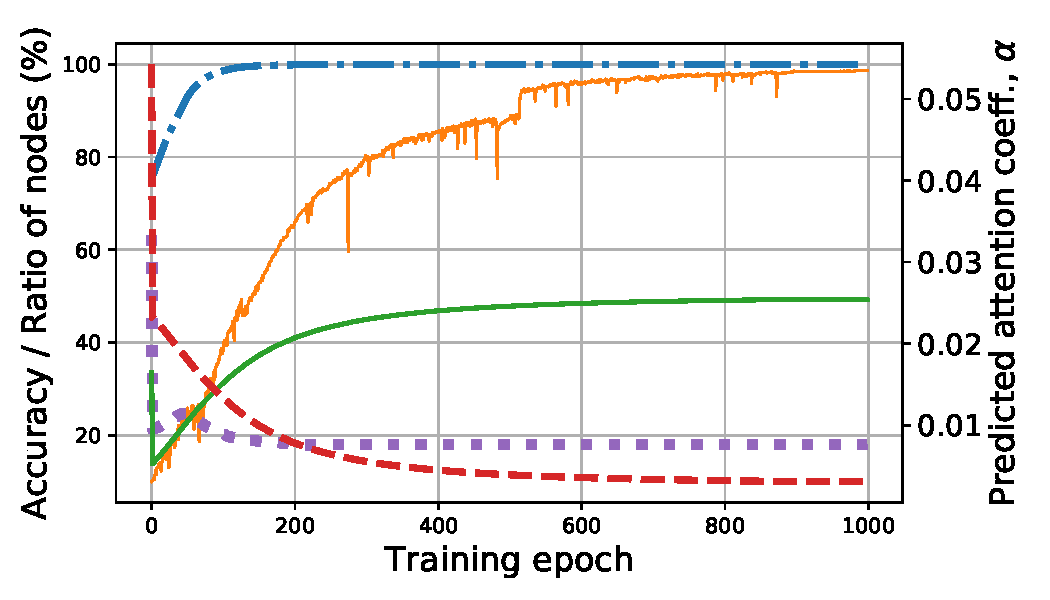
\includegraphics[width=\width, align=c, trim={0cm 0cm 0.5cm 0cm}, clip]{colors_init/bad_sup}} & %\hspace{0.5cm}
				{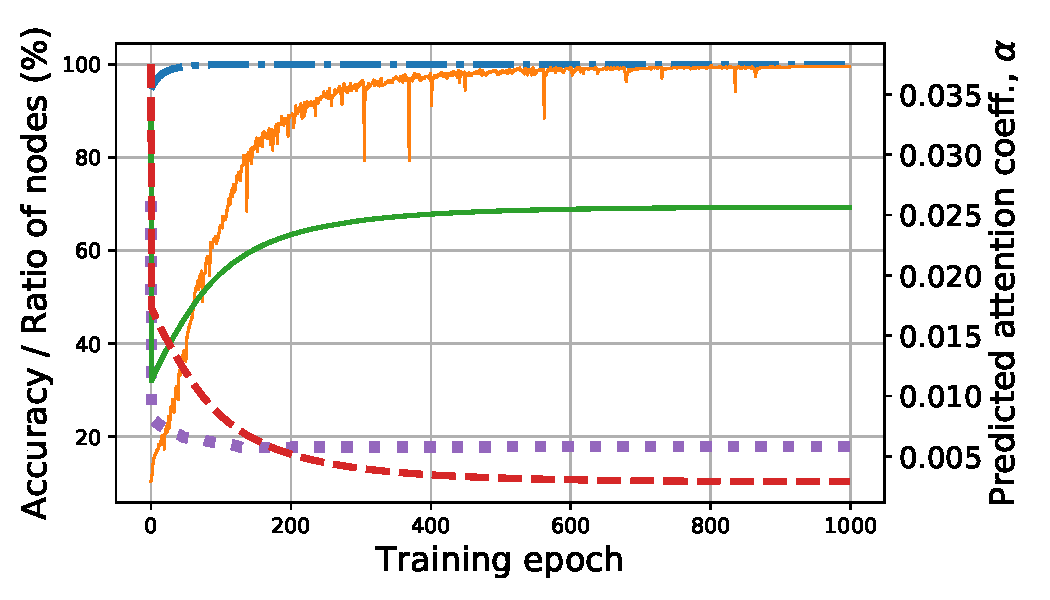
\includegraphics[width=\width, align=c, trim={0cm 0cm 0.5cm 0cm}, clip]{colors_init/good1_sup}} &
				{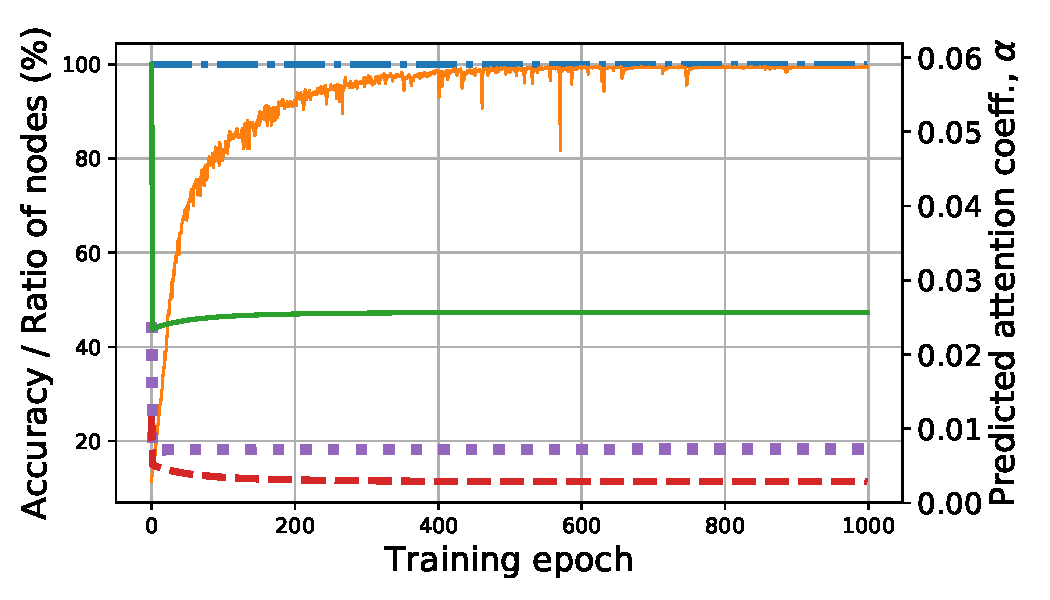
\includegraphics[width=\width, align=c, trim={0cm 0cm 0.5cm 0cm}, clip]{colors_init/optimal4_sup}} \\
				& (d) & (e) & (f) \\
			\end{tabular}
		\end{small}
		\vspace{-18pt}
	\end{center}
	\caption{\small Influence of initialization on training dynamics for \textsc{Colors} using GIN trained in unsupervised (a-c) and supervised (d-e) ways. The nodes that should be pooled according to our ground truth prior, must have larger attention values $\alpha$. However, in the unsupervised cases, only the model with an optimal initialization (c) reaches a high accuracy, while other models (a,b) are stuck in a suboptimal state and wrong nodes are pooled, which degrades performance. In the supervised cases (d-f), models converge to a perfect accuracy and initialization only affects the speed of convergence. In these experiments, we train models longer to see if they can recover from a bad initialization.}
	\label{fig:training_curves_unsup}
\end{figure}


\densepar{What are the factors influencing performance of \gnns with attention?}
We identify three key factors influencing performance of \gnns with attention: initialization of the attention model (i.e.~vector $\mathbf{p}$ or \gnn in \eqref{eq:attn_gcn}), strength of the main \gnn model (i.e.~the model that actually performs classification), and finally other hyperparameters of the attention and \gnn models.

We highlight initialization as the critical factor. We ran 100 experiments on \colors~with random initializations (\fig{\ref{fig:accuracy_cos_sim}}, \textit{(a-e)}) of the vector $\mathbf{p}$ and measured how performance of both attention and classification is affected depending on how close (in terms of cosine similarity) the initialized $\mathbf{p}$ was to the optimal one, $\mathbf{p} = [0,1,0]$.
We disentangle the dependency between the classification accuracy and cos.~sim. into two functions to make the relationship clearer (\fig{\ref{fig:accuracy_cos_sim}}, \textit{(a, c)}).
Interestingly, we found that classification accuracy depends \textit{exponentially} on attention correctness and becomes close to 100\% only when attention is also close to being perfect. In the case of slightly worse attention, even starting from 99\%, classification accuracy drops significantly.
This is an important finding that can also be valid for other more realistic applications. In the \textsc{Triangles} task we only partially confirm this finding, because our attention models could not achieve AUC high enough to boost classification. However, by observing the upper bound results obtained by training with ground truth attention, we assume that this boost potentially should happen once attention becomes accurate enough.\looseness=-1

\begin{figure}[tbh]
	\begin{center}
		\small
		\setlength{\tabcolsep}{0pt}
		\begin{minipage}{.55\textwidth}
		\begin{tabular}{cccc}
			& \textsc{Test-Orig} & \textsc{Test-Noisy} & \textsc{Test-NoisyC} \\
			\rotatebox[origin=c]{90}{\tiny \textsc{Input}} &
			{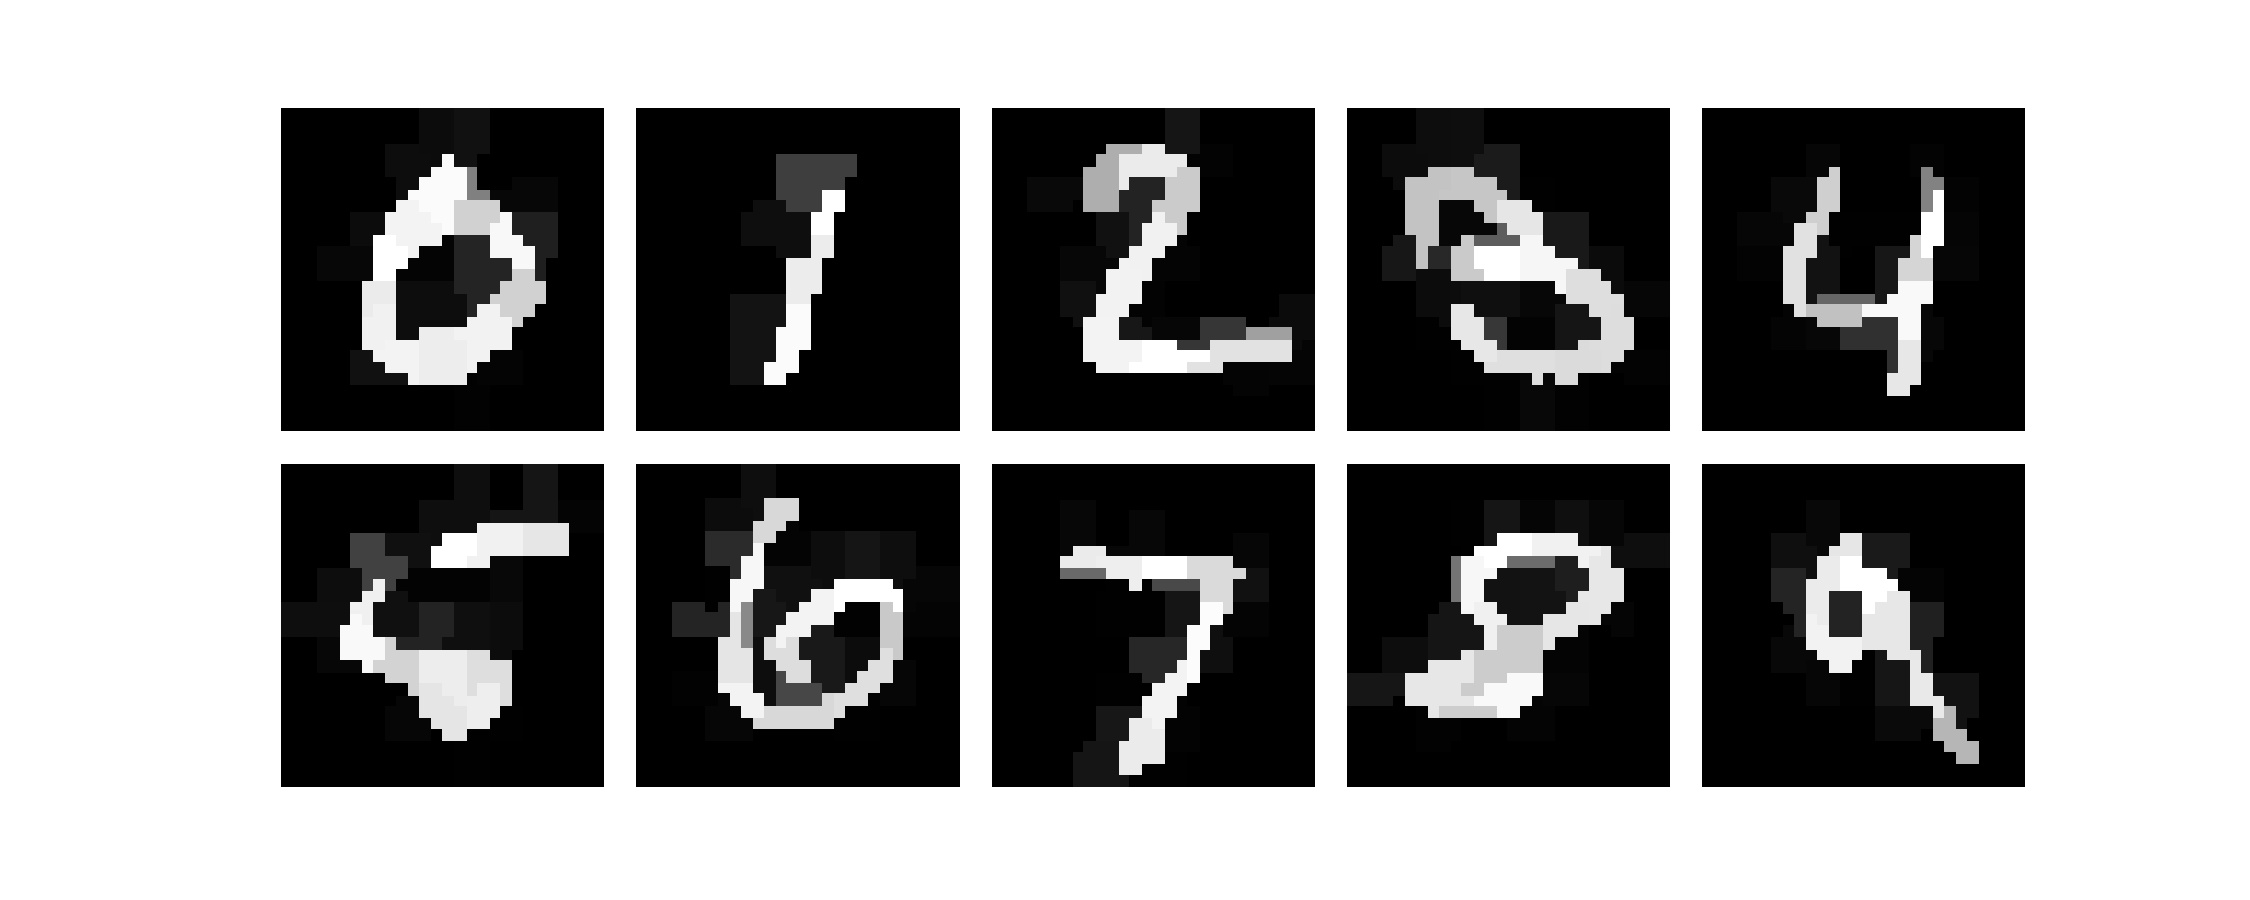
\includegraphics[width=0.3\textwidth, align=c, trim={4cm 1cm 3cm 1cm}, clip]{cheb_weak_sup/fig_0.pdf}} &
			{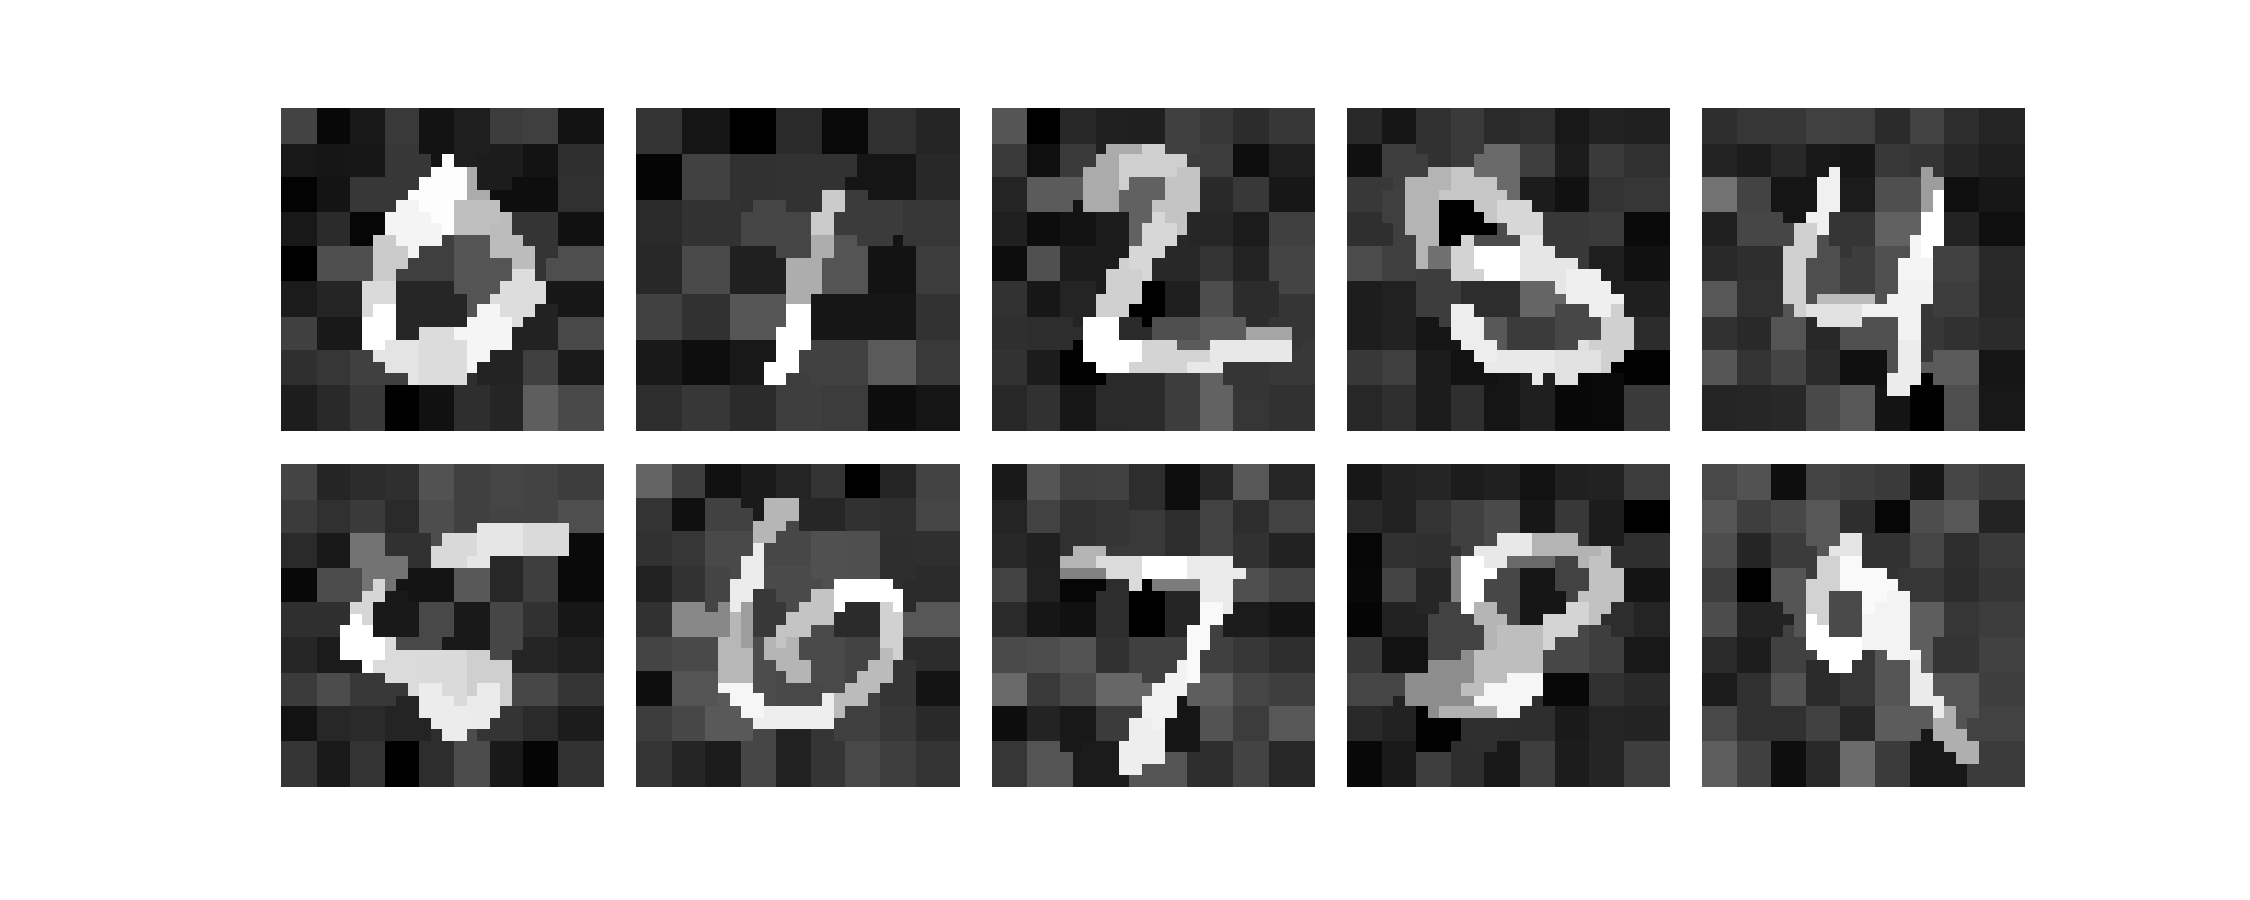
\includegraphics[width=0.3\textwidth, align=c, trim={4cm 1cm 3cm 1cm}, clip]{cheb_weak_sup/fig_1.pdf}} &
			{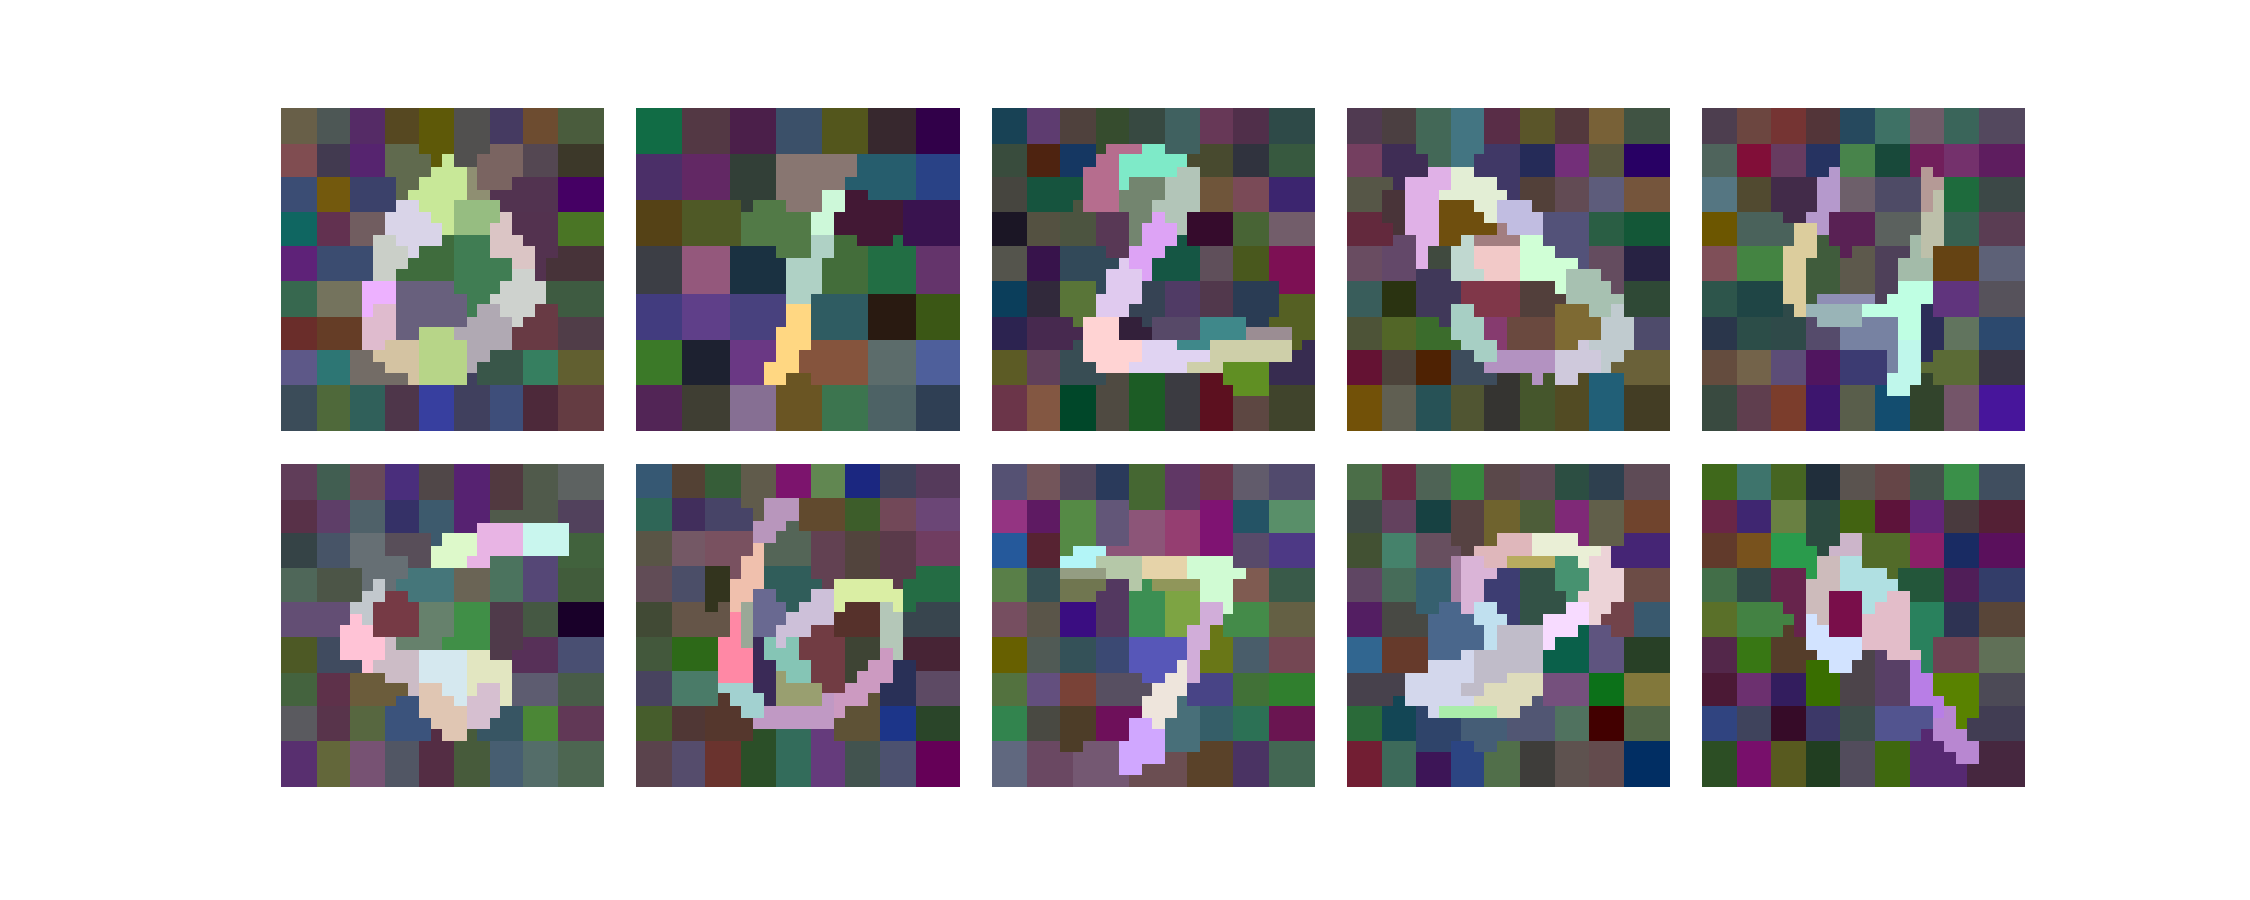
\includegraphics[width=0.3\textwidth, align=c, trim={4cm 1cm 3cm 1cm}, clip]{cheb_weak_sup/fig_2.pdf}} \\

			\rotatebox[origin=c]{90}{\tiny \textsc{DiffPool}} &
			{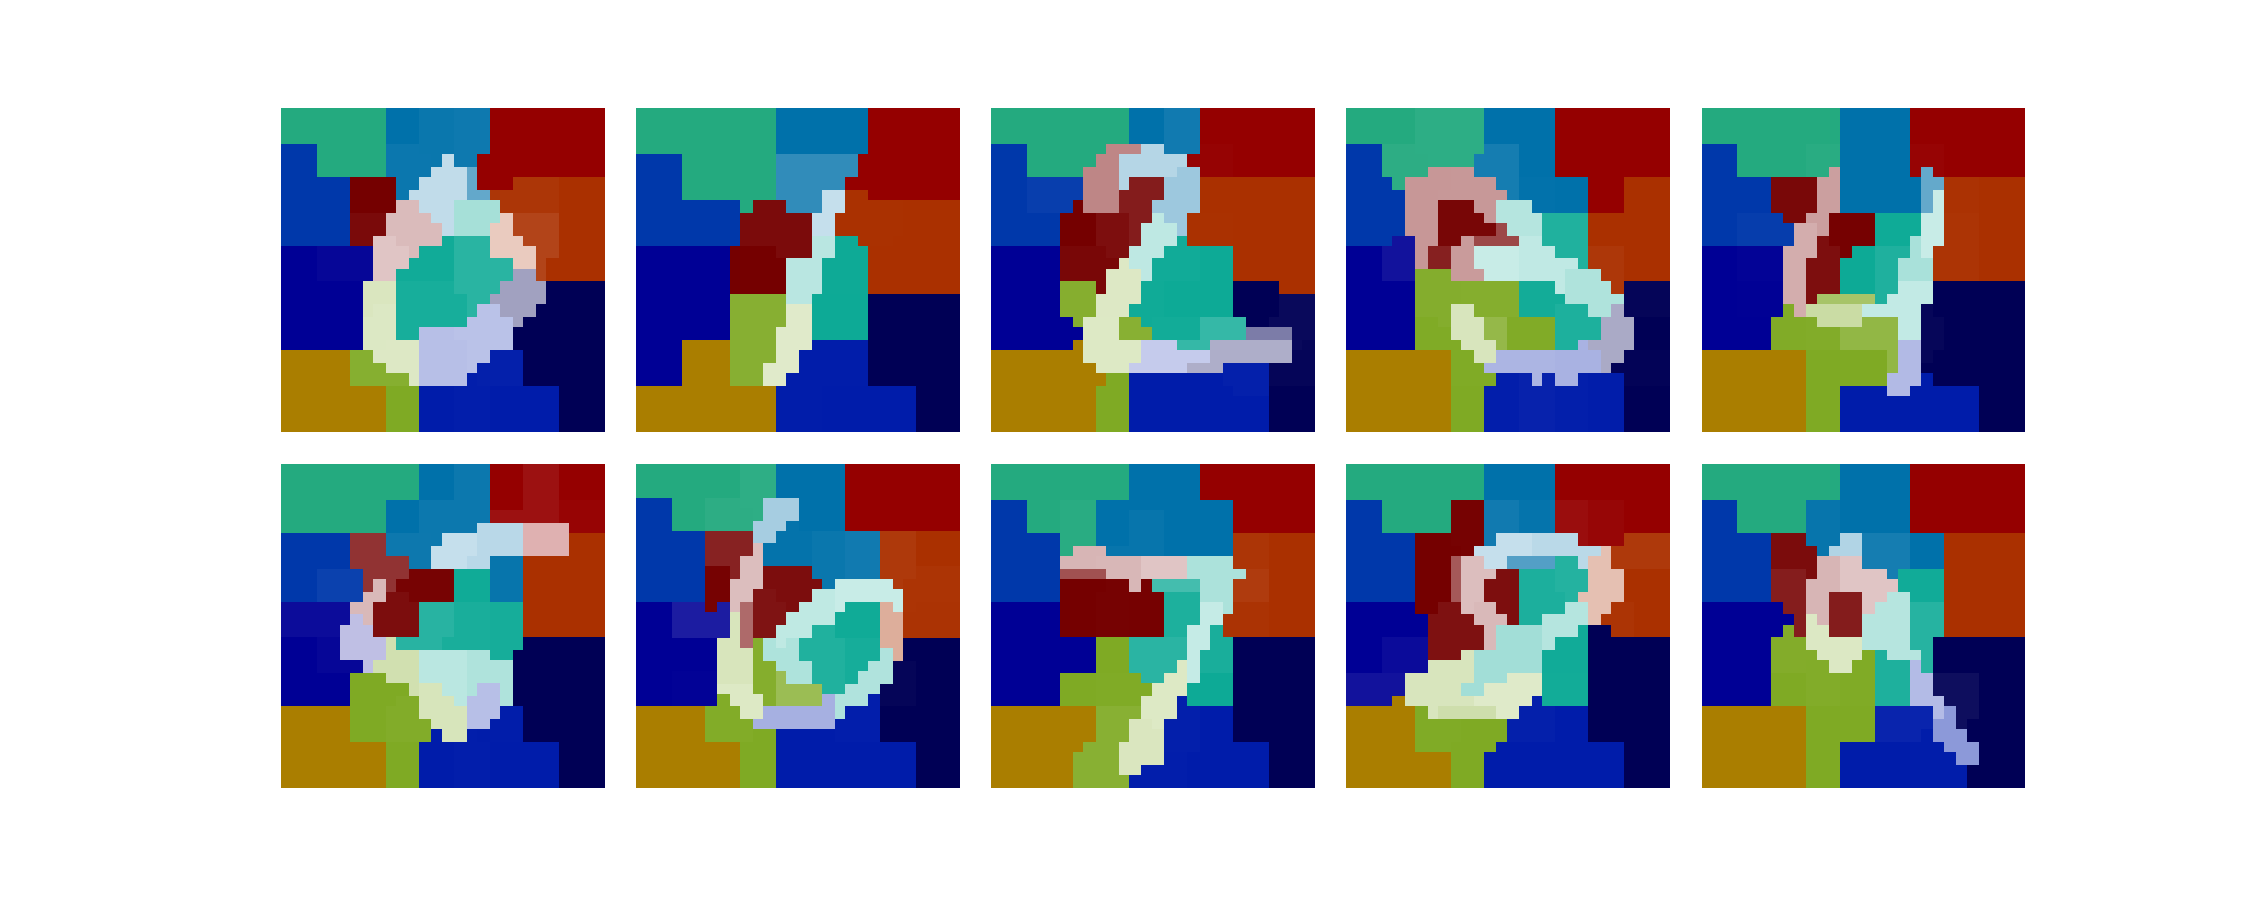
\includegraphics[width=0.3\textwidth, align=c, trim={4cm 1cm 3cm 1cm}, clip]{cheb_diff_pool_clusters/fig_diffpool_3.pdf}} &
			{\includegraphics[width=0.3\textwidth, align=c, trim={4cm 1cm 3cm 1cm}, clip]{cheb_diff_pool_clusters/fig_diffpool_4.pdf}} &
			{\includegraphics[width=0.3\textwidth, align=c, trim={4cm 1cm 3cm 1cm}, clip]{cheb_diff_pool_clusters/fig_diffpool_5.pdf}} \\

			\rotatebox[origin=c]{90}{$\mathbf{\alpha}^{WS}$} &
			{\includegraphics[width=0.3\textwidth, align=c, trim={4cm 1cm 3cm 1cm}, clip]{cheb_global_max_heat/fig_heat_3.pdf}} &
			{\includegraphics[width=0.3\textwidth, align=c, trim={4cm 1cm 3cm 1cm}, clip]{cheb_global_max_heat/fig_heat_3.pdf}} &
			{\includegraphics[width=0.3\textwidth, align=c, trim={4cm 1cm 3cm 1cm}, clip]{cheb_global_max_heat/fig_heat_5.pdf}} \\

			\rotatebox[origin=c]{90}{$\mathbf{\alpha}$} &
			{\includegraphics[width=0.3\textwidth, align=c, trim={4cm 1cm 3cm 1cm}, clip]{cheb_weak_sup/fig_3.pdf}} &
			{\includegraphics[width=0.3\textwidth, align=c, trim={4cm 1cm 3cm 1cm}, clip]{cheb_weak_sup/fig_4.pdf}} &
			{\includegraphics[width=0.3\textwidth, align=c, trim={4cm 1cm 3cm 1cm}, clip]{cheb_weak_sup/fig_5.pdf}} \\
		\end{tabular}
		\end{minipage}
%		\hspace{-2pt}
		\begin{minipage}{0.35\textwidth}
		\begin{tabular}{cc}
			\multicolumn{2}{c}{\textsc{Triangles Test-Large}} \rule[-7pt]{0pt}{0pt} \\
			{{\includegraphics[width=0.45\textwidth, align=c, trim={1cm 1cm 2cm 1.5cm}, clip]{cheb_weak_sup_triangles/triangles_test2_large.png}}} &
			{\includegraphics[width=0.5\textwidth, align=c, trim={2cm 1cm 0cm 1.5cm}, clip]{cheb_weak_sup_triangles/triangles_test2_gt_pool_large.pdf}} \\
			\tiny $N=93$ & \tiny $N=16$ \rule[-10pt]{0pt}{0pt} \\
			{\includegraphics[width=0.45\textwidth, align=c, trim={1cm 1cm 2cm 1.5cm}, clip]{cheb_weak_sup_triangles/triangles_test2_pred_large.png}} &
			{\includegraphics[width=0.5\textwidth, align=c, trim={2cm 1cm 0cm 1.5cm}, clip]{cheb_weak_sup_triangles/triangles_test2_pred_layer1_large.pdf}} \\
			\tiny $N=93$ & \tiny $N=27$ \\
		\end{tabular}
		\end{minipage}
	\end{center}
	\vspace{-10pt}
	\caption{\small Qualitative analysis. For \mnist~(on the left) we show examples of input test images (top row), results of DiffPool~\citep{ying2018hierarchical} (second row), attention weights $\mathbf{\alpha}^{WS}$ generated using a model with global pooling based on \eqref{eq:heat_maps} (third row), and $\mathbf{\alpha}$ predicted by our \wsup~model (bottom row). Both our attention-based pooling and DiffPool can be strong and interpretable depending on the task, but in our tasks DiffPool was inferior.
	For \tri~(on the right) we show an example of a test graph with $N=93$ nodes with six triangles and the results of pooling based on ground truth attention weights $\mathbf{\alpha}^{GT}$ (top row); in the bottom row we show attention weights predicted by our \wsup~model and results of our threshold-based pooling \eqref{eq:top-k_ours}. Note that during training, our model has not encountered noisy images (\mnist) nor graphs larger than with $N=25$ nodes (\tri). }
	\label{fig:attn_mnist}
	\vspace{-1pt}
\end{figure}

\densepar{Why is the variance of some results so high?}
In Table~\ref{table:results} we report high variance of results, which is mainly due to initialization of the attention model as explained above. This variance is also caused by initialization of other trainable parameters of a GNN, but we show that once the attention model is perfect, other parameters can recover from a bad initialization leading to better results. The opposite, however, is not true: we never observed recovery of a model with poorly initialized attention (\fig{\ref{fig:training_curves_unsup}}).\looseness=-1

\densepar{How top-k compares to our threshold-based pooling method?}
Our method to attend and pool nodes \eqref{eq:top-k_ours} is based on top-k pooling~\citep{graphunet2018} and we show that the proposed threshold-based pooling is superior in a principle way. When we use supervised attention our results are better by more than 40\% on \textsc{Colors-LargeC}, by 9\%  on \textsc{Triangles-Large} and by 3\% on \textsc{MNIST-75sp}. In \fig{\ref{fig:accuracy_cos_sim}} (\textit{(a,b)}-zoomed) we show that GIN and ChebyGIN models with supervised top-k pooling never reach an average accuracy of more than 80\% as opposed to our method which reaches 100\% in many cases.

\densepar{How results change with increase of attention model input dimensionality or capacity?}
We performed experiments using ChebyGIN-h - a model with higher dimensionality of an input to the attention model. In such cases, it becomes very unlikely to initialize it in a way close to optimal (\fig{\ref{fig:accuracy_cos_sim}}, \textit{(c-e)}), and attention accuracy is concentrated in the 60-80\% region. Effect of the attention model of such low accuracy is neglible or even harmful, especially on the large and noisy graphs. We also experimented with a deeper attention model (ChebyGIN-h), i.e. a 2 layer fully-connected layer with 32 hidden units for \colors~and \mnist, and a deeper \gnn \eqref{eq:attn_gcn} for \tri. This has a positive effect overall, except for \tri, where our attention models were already deep \gnns.\looseness-1

\begin{figure}[htpb]
	\vspace{-1pt}
	\setlength{\tabcolsep}{0pt}
	\begin{tabular}{ccccc}
		{\includegraphics[width=0.2\textwidth, align=c, trim={0cm 0cm 0cm 0cm}, clip]{init/unsup_colors3.pdf}} &
		{\includegraphics[width=0.2\textwidth, align=c, trim={0cm 0cm 0cm 0cm}, clip]{init/sup_colors3.pdf}} &
		{\includegraphics[width=0.2\textwidth, align=c, trim={0cm 0cm 0cm 0cm}, clip]{init/wsup_colors3.pdf}} &
		{\includegraphics[width=0.2\textwidth, align=c, trim={0cm 0cm 0cm 0cm}, clip]{init/acc_scale_cos_colors3.pdf}} &
		{\includegraphics[width=0.2\textwidth, align=c, trim={0cm 0cm 0cm 0cm}, clip]{init/acc_scale_cos_colors3_gcn.pdf}}
	\end{tabular}
	\caption{\small Influence of distribution parameters used to initialize the attention model $\mathbf{p}$ in the \colors~task with $n=3$ dimensional features. We show points corresponding to the commonly used initialization strategies of \ul{Xavier}~\citep{he2015delving} and \ul{Kaiming}~\citep{he2015delving}. \textit{(a-c)} Shaded areas show range, bars show $\pm1$ std.}
	\label{fig:init}
	\vspace{-10pt}
\end{figure}

\densepar{Can we improve initialization of attention?}
In all our experiments, we initialize $\mathbf{p}$ from the Normal distribution, ${\cal N}(0, 1)$. To verify if the performance can be improved by choosing another distribution, we evaluate GIN and GCN models on a wide range of random distributions, Normal ${\cal N}(0, \sigma)$ and Uniform $U(-\sigma, \sigma)$, by varying scale $\sigma$ (\fig{\ref{fig:init}}).
We found out that for unsupervised training (\fig{\ref{fig:init}}, \textit{(a)}), larger initial values and the Normal distribution should be used to make it possible to converge to an optimal solution, which is still unlikely and greatly depends on cosine similarity with GT attention (\fig{\ref{fig:init}}, \textit{(d,e)}). For supervised and ``weak-sup'' attention, smaller initial weights and either the Normal or Uniform distribution should be used (\fig{\ref{fig:init}}, \textit{(b,c)}).


\begin{table}[tbhp]%{R}{7.2cm}%[t]
	%\vspace{-12pt}
	\caption{\small \textbf{Results on the social (\collab) and molecule (\proteins~and \dd) datasets.} We use 3 layer GCNs~\citep{kipf2016semi} or ChebyNets~\citep{defferrard2016convolutional}. Dataset subscripts denote the maximum number of nodes in the training set according to our splits (\secref{\ref{sec:graph_data}}).\looseness-1}
	\vspace{-10pt}
	\scriptsize
	\label{table:results_graphs}
	\begin{center}
		%\setlength{\tabcolsep}{2.4pt}
		\begin{tabular}{lcccc}
			\toprule
			& \textbf{\collab}$_{35}$ & \textbf{\proteins}$_{25}$ & \textbf{\dd}$_{200}$ & \textbf{\dd}$_{300}$\Tstrut\Bstrut\\
			\midrule \\
			\# train / test graphs & 500 / 4500  & 500 / 613 & 462 / 716 & 500 / 678 \\
			\# nodes ($N$) train & 32-35 & 4-25 & 30-200 & 30-300 \\
			\# nodes ($N$) test & 32-492 & 6-620 & 201-5748 & 30-5748 \\
			\hline \\
			Global max & 65.9\std{3.4} & 74.4\std{1.0} & 29.7\std{4.9} & 72.7\std{3.6} \\
			Unsup, ours & 65.7\std{3.5} & 75.6\std{1.4} & 51.9\std{5.3} & 77.2\std{2.9} \\
			\hline \\
			Weak-sup & \textbf{67.0\std{1.7}} & \textbf{76.2\std{0.7}} &  \textbf{54.3\std{5.0}} & \textbf{78.4\std{1.1}} \\
			\bottomrule
		\end{tabular}
	\end{center}
	%\vspace{-8pt}
\end{table}




\begin{figure}[tbhp]
	\newcommand{\imgwidth}{0.17\textwidth}
	\begin{center}
		\small
		\setlength{\tabcolsep}{3pt}
		\begin{tabular}{cccccc}
			& \small \textsc{Global pool} & \small \textsc{Unsup} & \small \textsc{Unsup pooled} & \small \textsc{Weak-sup} &  \small \textsc{Weak-sup pooled} \\
			\rotatebox[origin=c]{90}{\small \collab$_{35}$} &
			{\includegraphics[width=\imgwidth, align=c, trim={0 0 0 0}, clip]{collab/56_96_32nodes_0_0_global.pdf}} &
			{\includegraphics[width=\imgwidth, align=c, trim={0 0 0 0}, clip]{collab/56_96_32nodes_0_1_unsup.pdf}} &
			{\includegraphics[width=\imgwidth, align=c, trim={0 0 0 0}, clip]{collab/56_96_21nodes_0_1_unsup_pooled.pdf}} &
			{\includegraphics[width=\imgwidth, align=c, trim={0 0 0 0}, clip]{collab/56_96_32nodes_0_0.pdf}} &
			{\includegraphics[width=\imgwidth, align=c, trim={0 0 0 0}, clip]{collab/56_96_14nodes_0_0_pooled.pdf}} \\ \\
			\rotatebox[origin=c]{90}{\small \proteins$_{25}$} &
			{\includegraphics[width=\imgwidth, align=c, trim={0 0 0 0}, clip]{proteins/46_437_134nodes_0_0_global.pdf}} &
			{\includegraphics[width=\imgwidth, align=c, trim={0 0 0 0}, clip]{proteins/46_437_134nodes_0_0_unsup.pdf}} &
			{\includegraphics[width=\imgwidth, align=c, trim={0 0 0 0}, clip]{proteins/46_437_79nodes_0_0_unsup_pooled.pdf}} &
			{\includegraphics[width=\imgwidth, align=c, trim={0 0 0 0}, clip]{proteins/46_437_134nodes_0_0.pdf}} &
			{\includegraphics[width=\imgwidth, align=c, trim={0 0 0 0}, clip]{proteins/46_437_72nodes_0_0_pooled.pdf}} \\ \\
			\rotatebox[origin=c]{90}{\small \dd$_{200}$} &
			{\includegraphics[width=\imgwidth, align=c, trim={0 0 0 0}, clip]{dd/65_640_212nodes_1_1_global.pdf}} &
			{\includegraphics[width=\imgwidth, align=c, trim={0 0 0 0}, clip]{dd/65_640_212nodes_1_1_unsup.pdf}} &
			{\includegraphics[width=\imgwidth, align=c, trim={0 0 0 0}, clip]{dd/65_640_70nodes_1_1_unsup_pooled.pdf}} &
			{\includegraphics[width=\imgwidth, align=c, trim={0 0 0 0}, clip]{dd/65_640_212nodes_1_1.pdf}} &
			{\includegraphics[width=\imgwidth, align=c, trim={0 0 0 0}, clip]{dd/65_640_73nodes_1_1_pooled.pdf}} \\
		\end{tabular}
	\end{center}
	\vspace{-10pt}
	\caption{\small Qualitative results. In \collab, a graph represents an ego-network of a researcher, therefore \textit{center nodes} are important. In \proteins~and \dd, a graph is a protein and nodes are amino acids, so it is important to attend to a \textit{connected chain} of amino acids to distinguish an enzyme from a non-enzyme protein. Our \wsup~method attends to and pools more relevant nodes compared to global and unsupervised models, leading to better classification results. }
	\label{fig:attn_graphs}
\end{figure}

\densepar{What is the recipe for more powerful attention \gnns?}
We showed that \gnns with supervised training of attention are significantly more accurate and robust, although in case of a bad initialization it can take a long time to reach the performance of a better initialization.
However, supervised attention is often infeasible. We suggested an alternative approach based on \wsup~training and validated it on our synthetic (Table~\ref{table:results}) and real (Table~\ref{table:results_graphs}) datasets. In case of \synthetic~we can compare to both unsupervised and supervised models and conclude that our approach shows performance, robustness and relatively low variation  (i.e. sensitivity to initialization) similar to supervised models and much better than unsupervised models. In case of \real~we can only compare to unsupervised and global pooling models and confirm that our method can be effectively employed for a wide diversity of graph classification tasks and attends to more relevant nodes (Figures~\ref{fig:attn_mnist} and~\ref{fig:attn_graphs}). Tuning the distribution and scale $\sigma$ for the initialization of attention can further improve results. For instance, on \proteins~for the \wsup~case, we obtain 76.4\% as opposed to 76.2\%.\looseness-1

\section{Conclusion}
%\vspace{-10pt}
We have shown that learned attention can be extremely powerful in graph neural networks, but only if it is close to optimal. This is difficult to achieve due to the sensitivity of initialization, especially in the unsupervised setting where we do not have access to ground truth attention. Thus, we have identified initialization of attention models for high dimensional inputs as an important open issue.
We also show that attention can make \gnns more robust to larger and noisy graphs, and that the weakly-supervised approach proposed in our work brings advantages similar to the ones of supervised models, yet at the same time can be effectively applied to datasets without annotated attention.

\vfill
\clearpage


\graphicspath{{Ch4_2020_bmvc/figs/}}

\chapter{{Graph Density-Aware Losses for Novel Compositions in Scene Graph Generation}\label{ch:bmvc2020}}

%\chapter{PROLOGUE TO SECOND ARTICLE}
\section*{Prologue}
\addcontentsline{toc}{section}{Prologue}

% \begin{tabular}{p{0.16\linewidth}p{0.78\linewidth}}
%      \textit{Title:} & Graph Density-Aware Losses for Novel Compositions in Scene Graph Generation \\
%      \textit{Authors:} & Boris Knyazev, Harm de Vries, Cătălina Cangea, Graham Taylor, Aaron Courville, Eugene Belilovsky \\
%      \textit{Published at:} & \venue{British Machine Vision Conference (BMVC 2020)} \\
%     \textit{Code release:} & \url{https://github.com/bknyaz/sgg} \\
%     \textit{Personal contributions:} & developed the key components of algorithms and models; developed the code; designed
% and ran all experiments; wrote most of the article.
% \end{tabular}

\vspace{10pt}
\densepar{Context.}
Visual recognition models have been greatly improved across different applications largely due to the advances in convolutional neural networks (\cnns). Scene graph generation (SGG) is a task where objects and the relationships between them must be recognized from images~\citep{xu2017scene}. Many state of the art SGG models have tuned their performance for frequent compositions of objects and relationships~\citep{zellers2018neural}. Unfortunately, there is an extreme reduction in performance of these models on rare or unseen compositions~\citep{tang2020unbiased}. Understanding and addressing this problem in a realistic large-scale setup is challenging yet needed to increase the  practical value of SGG models.\looseness-1

\densepar{Contributions.}
We analyzed the loss function typically used to train SGG models and found that it ignores an important property of visual scene graphs --- graph density (number of edges \wrt the number of nodes). To address this issue, we developed a loss with terms that are normalized according to the graph density. The SGG models trained with our graph-density normalized loss significantly improve in generalization to rare and unseen compositions.

\densepar{Recent works.}
\citet{tang2020unbiased} proposed a method based on causal inference to ``debias'' SGG models and improve generalization. In line with our work, \citet{suhail2021energy} proposed an improved loss function based on energy defined on graphs. \citet{khandelwal2021segmentation} added more precise object representation in the form of segmentation masks that also improved compositional generalization. \citet{liu2021fully} proposed relation affinity fields to better generalize to unseen/rare compositions. While these approaches are applied to the SGG task, object-centric learning is a more general-purpose method that can potentially improve generalization in a larger variety of visual tasks~\citep{locatello2020object,dittadi2021generalization}.

\section{Introduction}

In recent years, there has been growing interest to connect successes in visual perception with language and reasoning~\citep{su2019vl,zhou2019unified}. This requires us to design systems that can not only recognize objects, but understand and reason about the relationships between them. 
This is essential for such tasks as visual question answering (VQA)~\citep{antol2015vqa,hudson2019gqa,cangea2019videonavqa} or caption generation~\citep{yang2019auto, gu2019unpaired}. 
However, predicting a high-level semantic output (\eg~answer) from a low-level visual signal (\eg~image) is challenging due to a vast gap between the modalities.
To bridge this gap, it would be useful to have some intermediate representation that can be relatively easily generated by the low-level module and, at the same time, can be effectively used by the high-level reasoning module.
We want this representation to semantically describe the visual scene in terms of objects and relationships between them, which leads us to a structured image representation, the \textbf{scene graph} (SG)~\citep{johnson2015image, Krishna_2017}.
A scene graph is a collection of visual relationship \textit{triplets}: <\textit{subject}, \textit{predicate}, \textit{object}> (\eg~<cup, on, table>). Each node in the graph corresponds to a subject or object (with a specific image location) and edges to predicates~(\fig{\ref{fig:overview}}). 
Besides bridging the gap, SGs can be used to verify how well the model has understood the visual world, as opposed to just exploiting one of the biases in a dataset~\citep{jabri2016revisiting,anand2018blindfold,bahdanau2018systematic}.
Alternative directions to SGs include, for example, attention~\citep{norcliffe2018learning} and neural-symbolic models~\citep{vedantam2019probabilistic}.\looseness-1

\begin{figure}[t]
	\centering
	\begin{scriptsize}
		\setlength{\tabcolsep}{1pt}
		\begin{tabular}{c} \includegraphics[width=0.99\textwidth,align=c,trim={0 0.2cm 0 0.2cm},clip]{cup_on_surfboard_overview1.pdf} \\
		\end{tabular}
	\end{scriptsize}
	\vspace{-5pt}
	\caption{\small In this work, we improve scene graph generation $P({\cal G} | I)$. In many downstream tasks, such as VQA, the result directly depends on the accuracy of predicted scene graphs.}
	\label{fig:overview}
\end{figure}

\begin{figure}
	\scriptsize
	\centering
	\setlength{\tabcolsep}{3pt}
	{
		\begin{minipage}{0.5\linewidth}
			\hspace{-20pt}
			\begin{tabular}{cc}
				\multicolumn{2}{c}{{\hspace{30pt}\includegraphics[width=0.95\textwidth,trim={3.5cm 8.3cm 7cm 0.8cm},clip]{legend.pdf}}} \vspace{-3pt} \\
				\vspace{-3pt}
				\includegraphics[align=c,height=2.7cm]{large_graphs_train_labels.pdf} &
				\includegraphics[align=c,height=2.7cm]{large_graphs_vs_recall_predcls_zs.pdf} \\
				\hspace{20pt} (a) & \hspace{20pt} (b) 
			\end{tabular}
		\end{minipage}
	}
	\hspace{10pt}
	{
		\begin{minipage}{0.4\linewidth}
			\vspace{8pt}
			\begin{tabular}{p{3cm}p{3cm}}
				\centering
				\includegraphics[height=2cm, align=c]{2409758_stanford_nolabel.png} & \includegraphics[height=2cm, align=c]{1160208_stanford_nolabel.png} \Bstrut \\ 
				\centering (c) Image with a small scene graph & \centering (d) Image with a large scene graph
			\end{tabular}
		\end{minipage}
	}
	\vspace{-3pt}
	\caption{\small \textbf{Motivation of our work.} We split the training set of Visual Genome~\citep{Krishna_2017} into two subsets: those with relatively small ($\leq 10$ nodes) and large ($>10$ nodes) graphs. (\textbf{a}) While each subset contains a similar number of images (the three left bars), larger graphs contain more few-shot labels (the three right bars). (\textbf{b}) Baseline methods (\citep{xu2017scene} in this case) fail to learn from larger graphs due to their loss function. However, training on large graphs and corresponding few-shot labels is important for stronger generalization. We address this limitation and significantly improve results on zero and few-shots. (\textbf{c, d}) Small and large scene graphs typically describe simple and complex scenes respectively. \looseness-1 
	}
	%\vspace{-10pt}
	\label{fig:motivation}
\end{figure}


\textbf{Scene graph generation} (SGG) is the task of predicting a SG given an input image. The inferred SG can be used directly for downstream tasks such as VQA~\citep{zhang2019empirical,NSM2019}, image captioning~\citep{yang2019auto, gu2019unpaired} or retrieval~\citep{johnson2015image,belilovsky2017joint,tang2020unbiased}.
A model which performs well on SGG should demonstrate the ability to ground visual concepts to images and generalize to compositions of objects and predicates in new contexts. In real world images, some compositions (\eg~<cup, on, table> ) appear more frequently than others (\eg~<cup, on, \textit{surfboard}> or <cup, \textit{under}, table>), which creates a strong frequency bias. This makes it particularly challenging for models to generalize to novel (zero-shot) and rare (few-shot) compositions, even though each of the subjects, objects and predicates have been observed at training time.
The problem is exacerbated by the test set and evaluation metrics, which do not penalize models that blindly rely on such bias. Indeed,~\citet{zellers2018neural} has pointed out that SGG models largely exploit simple co-occurrence information. In fact, the performance of models predicting solely based on frequency  (i.e. a cup is most likely to be \textit{on} a \textit{table}) is not far from the state-of-the-art using common metrics (see \textsc{Freq} in Table~\ref{table:main_results}).\looseness-1

In this work, we reveal that (a) the frequency bias exploited by certain  models leads to poor generalization on few-shot and zero-shot compositions; (b) existing models disproportionately penalize large graphs, even if these often contain many of the infrequent visual relationships, which leads to performance degradation on few and zero-shot cases (\fig{\ref{fig:motivation}}). We address these challenges and show that our suggested improvements can provide benefits for two strong baseline models~\citep{xu2017scene,zellers2018neural}. Overall, we make the following four \textbf{contributions}:

\begin{enumerate}[leftmargin=10pt,labelsep=2pt]
	\itemsep0em 
	\item \textbf{Improved loss}: we introduce a density-normalized edge loss, which improves results on all metrics, especially for few and zero-shots (\secref{\ref{sec:loss_norm}});
	\item \textbf{Novel weighted metric}: we illustrate several issues in the evaluation of few and zero-shots, proposing a novel weighted metric which can better track the performance of this critical desiderata (\secref{\ref{sec:metric}});
	\item \textbf{Frequency bias}: we demonstrate a negative effect of the frequency bias, proposed in Neural Motifs~\citep{zellers2018neural}, on few and zero-shot performance (\secref{\ref{sec:experiments}}); 
	\item \textbf{Scaling to GQA}: in addition to evaluating on Visual Genome (VG)~\citep{Krishna_2017}, we confirm the usefulness of our loss and metrics on GQA~\citep{hudson2019gqa} -- an improved version of VG. GQA has not been used to evaluate SGG models before and is interesting to study, because compared to VG its scene graphs are cleaner, larger, more dense and contain a larger variety of objects and predicates (\secref{\ref{sec:experiments}}).
\end{enumerate}
\vspace{-10pt}


\section{Related work}

\textbf{Zero-shot learning.}
In vision tasks, such as image classification, zero-shot learning has been extensively studied, and the main approaches are based on attributes~\citep{lampert2013attribute} and semantic embeddings~\citep{frome2013devise, xian2016latent}.
The first approach is related to the zero-shot problem we address in this work: it assumes that all individual attributes of objects (color, shape, etc.) are observed during training, such that novel classes can be detected at test time based on \textit{compositions} of their attributes.
Zero-shot learning in scene graphs is similar: all individual subjects, objects and predicates are observed during training, but most of their compositions are not. This task was first evaluated in~\citep{lu2016visual} on the VRD dataset using a joint vision-language model. 
Several follow-up works attempted to improve upon it: by learning a translation operator in the embedding space~\citep{zhang2017visual}, clustering in a weakly-supervised fashion~\citep{peyre2017weakly}, using conditional random fields~\citep{cong2018scene} or optimizing a cycle-consistency loss to learn object-agnostic features~\citep{yang2018shuffle}.
Augmentation using generative networks to generate more examples of rare cases is another promising approach~\citep{wang2019generating}; but, it was only evaluated in the predicate classification task. In our work, we also consider subject/object classification to enable the classification of the whole triplets, making the ``image to scene graph'' pipeline complete. Most recently,~\citet{tang2020unbiased} proposed learning causal graphs and showed strong performance in zero-shot cases.

While these works improve generalization, none of them has identified the challenges and importance of learning from large graphs for generalization. By concentrating the model's capacity on smaller graphs and neglecting larger graphs, baseline models limit the variability of training data, useful for stronger generalization~\citep{hill2019environmental}. Our loss enables this learning, increasing the effective data variability. Moreover, previous gains typically incur a large computational cost, while our loss has negligible cost and can be easily added to other models.\looseness-1


\textbf{Few-shot predicates.} 
Several recent works have addressed the problem of imbalanced and few-shot predicate classes ~\citep{chen2019knowledge, dornadula2019visual,tang2019learning,zhang2019graphical,tang2020unbiased,chen2019scene}. However, compared to our work, these works have not considered the imbalance between foreground and background edges, which is more severe than other predicate classes (\fig{\ref{fig:pred_distr}}) and is important to be fixed as we show in this work.
Moreover, we argue that the compositional generalization, not addressed in those works, can be more difficult than generalization to rare predicates. For example, the triplet <cup, on, surfboard> is challenging to be predicted correctly as a whole; even though `on' can be the most frequent predicate, it has never been observed together with `cup' and `surfboard'. Experimental results in previous work~\citep{lu2016visual,zhang2017visual,yang2018shuffle,wang2019generating,tang2020unbiased} highlight this difficulty. Throughout this work, by ``few-shot'' we assume triplets, not predicates.

\textbf{``Unbiasing'' methods.}
Our idea is similar to the Focal loss~\citep{lin2017focal}, which addresses the imbalance between foreground and background objects in the object detection task. However, directly applying the focal loss to Visual Genome is challenging, due to the large amount of missing and mislabeled examples in the dataset. In this case, concentrating the model's capacity on ``hard'' examples can be equivalent to putting more weight on noise, which can hurt performance. \citet{tang2020unbiased} compared the focal loss and other unbiasing methods, such as upsampling and upweighting, and did not report significantly better results.


\section{Methods}
\label{sec:methods}
In this section, we will review a standard loss used to train scene graph generation models (\secref{\ref{sec:baseline}}) and describe our improved loss (\secref{\ref{sec:loss_norm}}). We will then discuss issues with evaluating rarer combinations and propose a new weighted metric (\secref{\ref{sec:metric}}). 



\subsection{Overview of scene graph generation}
\label{sec:baseline}
In scene graph generation, given an image $I$, we aim to output a scene graph ${\cal G}=(O,R)$ consisting of a set of subjects and objects ($O$) as nodes and a set of relationships or predicates ($R$) between them as edges (\fig{\ref{fig:overview}}). So the task is to maximize the probability $P({\cal G} | I)$, which can be expressed as  $P(O,R | I) = P(O |I)\ P(R | I,O)$.
Except for works that directly learn from pixels~\citep{newell2017pixels}, the task is commonly~\citep{xu2017scene,yang2018graph,zellers2018neural} reformulated by first detecting bounding boxes $B$ and extracting corresponding object and edge features, $V=f(I,B)$ and $E=g(I,B)$ respectively, using some functions $f,g$ (\eg~a ConvNet followed by ROI Align~\citep{he2017mask}):
\begin{equation}
\label{eq:scene_graph_prob_box}
P({\cal G} |I) = P(V,E |I)\ P(O,R | V,E,I).%
\end{equation}
The advantage of this approach is that solving $P(O,R | V,E,I)$ is easier than solving $P(O,R | I)$. At the same time, to compute $P(V,E |I)$ we can use pretrained object detectors~\citep{ren2015faster, he2017mask}.
Therefore, we follow~\citep{xu2017scene,yang2018graph,zellers2018neural} and use this approach to scene graph generation.

In practice, we can assume that the pretrained object detector is fixed or that ground truth bounding boxes $B$ are available, so we can assume $P(V,E|I)$ is constant. In addition, following~\citep{lu2016visual,xu2017scene,yang2018graph}, we can assume conditional independence of variables $O$ and $R$: $P(O,R|V,E,I)=P(O|V,E,I)P(R|V,E,I)$. We thus obtain the scene graph generation loss:
\begin{equation}
\label{eq:scene_graph_prob_simple}
-\text{log} P({\cal G} |I) = -\text{log} P(O | V,E,I) - \text{log} P(R | V,E,I).
\end{equation}
Some models~\citep{zellers2018neural,zhang2019graphical} do not assume the conditional independence of $O$ and $R$, making predicates explicitly depend on subject and object labels: $P(O,R|V,E,I)=P(O|V,E,I) P(R|O,V,E,I)$. However, such a model must be carefully regularized, since it can start to ignore $(V,E,I)$ and mainly rely on the frequency distribution $P(R|O)$ as a stronger signal. For example, the model can learn that between `cup' and `table' the relationship is most likely to be `on', regardless the visual signal. As we show, this can hurt generalization.\looseness-1

\begin{wrapfigure}{r}{5.7cm}%
	\vspace{-10pt}
	\centering
	\includegraphics[width=5.5cm,align=c]{rel_distr_train_VG.pdf} \\
	\vspace{-5pt}
	\caption{\small Predicate distribution in Visual Genome (split~\citep{xu2017scene}). BG edges (note the log scale) dominate, with >96\% of all edges, creating an extreme imbalance. For clarity, only some most and least frequent predicate classes are shown.\looseness-1}
	\label{fig:pred_distr}
	%\vspace{-20pt}
\end{wrapfigure}

\eqref{eq:scene_graph_prob_simple} is commonly handled as a multitask classification problem, where each task is optimized by the cross-entropy loss ${\cal L}$.
In particular, given a batch of scene graphs with $N$ nodes and $M$ edges in total, the loss is the following:
\begin{equation}
\label{eq:loss_baseline}
{\cal L} = {\cal L}_{node} + {\cal L}_{edge} = \frac{1}{N}\sum_i^N{\cal L}_{obj,i} + \frac{1}{M}\sum_{ij}^M {\cal L}_{rel,ij}.
\end{equation}
Node and edge features $(V,E)$ output by the detector form a complete graph without self-loops (\fig{\ref{fig:overview}}). So, conventionally~\citep{xu2017scene,yang2018graph,zellers2018neural}, the loss is applied to all edges: $M \approx N^2$.
These edges can be divided into foreground (FG), corresponding to annotated edges, and background (BG), corresponding to not annotated edges: $M = M_{FG} + M_{BG}$.
The BG edge type is similar to a ``negative'' class in the object detection task and has a similar purpose.
Without training on BG edges, at test time the model would label all pairs of nodes as ``positive'', i.e. having some relationship, when often it is not the case (at least, given the vocabulary in the datasets). Therefore, not using the BG type can hurt the quality of predicted scene graphs and can lower recall.\looseness-1

\subsection{Hyperparameter-free normalization of the edge loss}
\label{sec:loss_norm}

\textbf{Baseline loss as a function of graph density.}
In scene graph datasets such as Visual Genome, the number of BG edges is greater than FG ones (\fig{\ref{fig:pred_distr}}), yet the baseline loss~\eqref{eq:loss_baseline} does not explicitly differentiate between BG and other edges. If we assume a fixed probability for two objects to have a relationship, then as the number of nodes grows we can expect fewer of them to have a relationship. Thus the graph density can vary based on the number of nodes (\fig{\ref{fig:graph_density}}), a fact not taken into account in \eqref{eq:loss_baseline}.
To avoid this, we start by decoupling the edge term of~\eqref{eq:loss_baseline} into the foreground (FG) and background (BG) terms:\looseness-1
%
\begin{equation}
{\cal L}_{edge} = \frac{1}{M}\sum_{ij}^M{\cal L}_{rel,ij} =  \frac{1}{M_{FG} + M_{BG}} \bigg[ \underbrace{\sum\nolimits_{ij \in \cal E}^{M_{FG}}{\cal L}_{rel,ij}}_{\text{FG edges}} + \underbrace{\sum\nolimits_{ij \notin \cal E}^{M_{BG}}{\cal L}_{rel,ij}}_{\text{BG edges}} \bigg]  ,
\end{equation}
%
\noindent where ${\cal E}$ is a set of FG edges, $M_{FG}$ is the number of FG edges ($|{\cal E}|$) and $M_{BG}$ is the number of BG edges.
Next, we denote FG and BG edge losses averaged per batch as ${\cal L}_{FG}=1/M_{FG}\sum_{ij \in \cal E}^{M_{FG}}{\cal L}_{rel,ij}$ and ${\cal L}_{BG}=1/M_{BG}\sum_{ij \notin \cal E}^{M_{BG}}{\cal L}_{rel,ij}$, respectively.
Then, using the definition of graph density as a proportion of FG edges to all edges, $d=M_{FG} / (M_{BG} + M_{FG})$, we can express the total baseline loss equivalent to \eqref{eq:loss_baseline} \textbf{as a function of graph density}:\looseness-1
%
\begin{equation}
\label{eq:loss_decouple}
\boxed{
	{\cal L} = {\cal L}_{node} + d {\cal L}_{FG}  + (1 - d) {\cal L}_{BG}.}
\end{equation}


\noindent\textbf{Density-normalized edge loss.}
\eqref{eq:loss_decouple} and \fig{\ref{fig:graph_density}} allow us to notice two issues:

\begin{enumerate}[leftmargin=10pt,labelsep=2pt]%
	\itemsep0em 
	\item \textbf{Discrepancy of the loss between graphs of different sizes.} Since $d$ exponentially decreases with graph size (~\ref{fig:graph_density}, left), FG edges of larger graphs are weighted less than edges of smaller graphs in the loss (\fig{\ref{fig:graph_density}}, middle), making the model neglect larger graphs.\looseness-1
	
	\item \textbf{Discrepancy between object and edge losses.}
	Due to $d$ tending to be small on average, $L_{edge}$ is much smaller than $L_{node}$, so the model might focus mainly on $L_{node}$ (\fig{\ref{fig:graph_density}}, right).\looseness-1
\end{enumerate}

\vspace{-5pt}
Both issues can be addressed by normalizing FG and BG terms by graph density $d$:
\begin{equation}
\label{eq:loss_norm}
\boxed{{\cal L} = {\cal L}_{node} + \gamma \big[ {\cal L}_{FG}  + {M_{BG}}/{M_{FG}} {\cal L}_{BG}\big].}
\end{equation}
\noindent where $\gamma=1$ in our default hyperparameter-free variant and $\gamma \neq 1$ only to empirically analyze the loss (Table~\ref{table:loss_ablations}). Even though the BG term still depends on graph density, we found it to be less sensitive to variations in $d$, since the BG loss quickly converges to some stable value, performing a role of regularization (\fig{\ref{fig:graph_density}}, right).
We examine this in detail in \secref{\ref{sec:experiments}}.

\begin{figure}%[h]
	\centering
	\begin{small}
		\setlength{\tabcolsep}{1pt}
		\begin{tabular}{ccc}
			\includegraphics[width=0.3\textwidth,align=c]{VG_graphs_bg_b1.pdf} &
			\includegraphics[width=0.3\textwidth,align=c]{loss_adaptive4_b6_graphsize.pdf} & \includegraphics[width=0.3\textwidth,align=c]{losses_vs_iter_loss_adaptive4_b6.pdf} \\ $d \rightarrow 0 $ for large graphs & Large graphs are downweighted by $d$ & $L_{edge} \ll L_{node}$ \\
		\end{tabular}
	\end{small}
	%\vspace{-5pt}
	\caption{
		\small (\textbf{left}) The number of FG edges grows much more slowly with graph size than the number of BG edges (on VG: $M_{FG}\approx 0.5N$). This leads to: (\textbf{middle}) Downweighting of the FG loss on larger graphs and effectively limiting the amount and variability of training data, since large graphs contain a lot of labeled data (\fig{\ref{fig:motivation}}); here, losses of converged models for batches sorted by graph size are shown. (\textbf{right}) Downweighting of the edge loss $L_{edge}$ overall compared to $L_{node}$, even though both tasks are equally important to correctly predicting a scene graph. Our normalization fixes both issues.}
	\label{fig:graph_density}
\end{figure}

\subsection{Weighted triplet recall}
\label{sec:metric}

The common evaluation metric for scene graph prediction is image-level Recall@K or R@K \citep{xu2017scene, yang2018graph, zellers2018neural}.
To compute it, we first need to extract the top-$K$ triplets, $\text{Top}_K$, from the \textit{entire image} based on ranked predictions of a model . Given a set of ground truth triplets, \text{GT}, the image-level R@K is computed as (see \fig{\ref{fig:eval}} for a visualization): 
%\setlength{\abovedisplayskip}{3pt}
%\setlength{\belowdisplayskip}{3pt}
\begin{equation}
\label{eq:recall_image}
\text{R}@\text{K} = {|\text{Top}_K \cap \text{GT}|}/{|\text{GT}|}.
\end{equation}
There are four issues with this metric:
%(we discuss additional details in~\apdx):

\begin{enumerate}[label=(\alph*),wide, labelindent=0pt, leftmargin=0pt, listparindent=0pt, labelsep=3pt]
	\itemsep0em 
	\item The frequency bias of triplets means more frequent triplets will dominate the metric.
	\item The denominator in~\eqref{eq:recall_image} creates discrepancies between images with different $|\text{GT}|$ (the number of ground truth triplets in an image), especially pronounced in few/zero shots.
	\item Evaluation of zero ($n=0$) and different few-shot cases $n=1,5,10,...$~\citep{wang2019generating} leads to many R@K results~\citep{wang2019generating}. This complicates the analysis. Instead, we want a single metric for all $n$.
	\item Two ways of computing the image-level recall~\citep{newell2017pixels,zellers2018neural}, graph \textit{constrained} and \textit{unconstrained}, lead to very different results and complicate the comparison (\fig{\ref{fig:eval}}).%
\end{enumerate}

To address issue \textbf{(a)}, the predicate-normalized metric, mean recall (mR@K)~\citep{chen2019knowledge,tang2019learning} and weighted mR@K were introduced~\citep{zhang2019graphical}. These metrics, however, only address the imbalance of predicate classes, not whole triplets.
Early work~\citep{lu2016visual,dai2017detecting} used triplet-level Recall@K (or R$_{tr}$@K) for some tasks (\eg~predicate detection), which is based on ranking predicted triplets for each ground truth subject-object pair independently; the pairs without relationships are not evaluated. Hence, R$_{tr}$@K is similar to top-$K$ accuracy.
This metric avoids issues \textbf{(b)} and \textbf{(d)}, but the issues of the frequency bias \textbf{(a)} and unseen/rare cases \textbf{(c)} still remain.
To alleviate these, we adapt this metric to better track unseen and rare cases. We call our novel metric Weighted Triplet Recall wR$_{tr}$@K, which computes a recall at each triplet and reweights the average result based on the frequency of the GT triplet in the training set: 
%\setlength{\abovedisplayskip}{3pt}
%\setlength{\belowdisplayskip}{3pt}
\begin{equation}
\label{eq:recall_triplet}
\text{wR}_{tr}@\text{K} =  \sum\nolimits_t^T w_t [\text{rank}_t \leq K],
\end{equation}
\noindent where $T$ is the number of all test triplets, $[\cdot]$ is the Iverson bracket, $w_t=\frac{1}{(n_t + 1)\sum_t 1/(n_t + 1)} \in [0,1]$ and $n_t$ is the number of occurrences of triplet $t$ in the training set; $n_t + 1$ is used to handle zero-shot triplets; $\sum_t w_t = 1$. Since wR$_{tr}$@K is still a triplet-level metric, we avoid issues \textbf{(b)} and \textbf{(d)}. Our metric is also robust to the frequency-bias \textbf{(a)}, since frequent triplets (with high $n_t$) are downweighted proportionally, which we confirm by evaluating the \textsc{Freq} model from~\citep{zellers2018neural}. Finally, a single wR$_{tr}$@K value shows zero and few-shot performance linearly aggregated for all $n \geq 0$, solving issue \textbf{(c)}. 

\begin{figure}%[h]
	\centering
% 	\vspace{-10pt}
	{\includegraphics[width=\textwidth]{metrics.pdf}}
	\vspace{-10pt}
	\caption{\small Existing image-level recall metrics \textit{versus} our proposed weighted triplet recall. We first make unweighted predictions $\text{rank}_t \leq K$ for all GT triplets in all test images, then reweight them according to the frequency distribution~\eqref{eq:recall_triplet}. Computing our metric per image would be noisy.
	}
	\label{fig:eval}
\end{figure}

\vspace{-5pt}
\section{Experiments}
\label{sec:experiments}
\vspace{-5pt}

\textbf{Datasets.}
We evaluate our loss and metric on Visual Genome~\citep{Krishna_2017}. Since it is a noisy dataset, several ``clean'' variants were introduced. We mainly experiment with the most common variant (VG)~\citep{xu2017scene}, which consists of the 150 most frequent object and 50 predicates classes. An alternative variant (VTE)~\citep{zhang2017visual} has been often used for zero-shot evaluation. Surprisingly, we found that the VG split~\citep{xu2017scene} is better suited for this task, given a larger variability of zero-shot triplets in the test set
%(see Table~\ref{table:datasets} in~\apdx). 
Recently, GQA~\citep{hudson2019gqa} was introduced, where scene graphs were cleaned to automatically construct question answer pairs. GQA has more object and predicate classes, so that zero and few-shot triplets are more likely to occur at test time. To the best of our knowledge, scene graph generation (SGG) results have not been reported on GQA before, even though some VQA models have relied on SGG~\citep{NSM2019}.\looseness-1

\textbf{Training and evaluation details.}
We experiment with two models: Message Passing (MP)~\citep{xu2017scene} and Neural Motifs (NM)~\citep{zellers2018neural}. We use publicly available implementations of MP and NM\footnote{\url{https://github.com/rowanz/neural-motifs}}, with all architecture details and hyperparameters kept the same. %(except for the small changes outlined in Table~\ref{table:arch} in~\apdx).
To be consistent with baseline models, for Visual Genome we use Faster R-CNN~\citep{ren2015faster} with VGG16 as a backbone to extract node and edge features. For GQA we choose a more recent Mask R-CNN~\citep{he2017mask} with ResNet-50-FPN as a backbone pretrained on COCO. We also use this detector on the VTE split.
We perform more experiments with Message Passing, since our experiments revealed that it better generalizes to zero and few-shot cases, while performing only slightly worse on other metrics. In addition, it is a relatively simple model, which makes the analysis of its performance easier.
We evaluate models on three tasks, according to~\citep{xu2017scene}: 1) predicate classification (\textbf{PredCls}), in which the model only needs to label a predicate given ground truth object labels and bounding boxes, i.e. $P(R|I,B,O)$; 2) scene graph classification (\textbf{SGCls}), in which the model must also label objects, i.e. $P(O,R|I,B)$; 3) scene graph generation \textbf{SGGen} (sometimes denoted as \textbf{SGDet}), $P({\cal G}|I)$, which includes detecting bounding boxes first (reported separately in Tables~\ref{table:sggen_results},~\ref{table:gqa_sgg}).

\subsection{Results}
Table~\ref{table:main_results} shows our main results, where for each task we report five metrics: image-level recall on all triplets (R@K) and zero-shot triplets (R$_{ZS}$@K), triplet-level recall (R$_{tr}$@K) and our weighted triplet recall (wR$_{tr}$@K), and mean recall (mR@K). We compute recalls without the graph constraint since
%, as we discuss in~\apdx, 
this is a more accurate metric. We denote graph-constrained results as \textbf{PredCls-GC}, \textbf{SGCls-GC}, \textbf{SGGen-GC} and report them only in Tables~\ref{table:zs_comparison_vte},~\ref{table:zs_comparison_vg} and Table~\ref{table:sggen_results}.


%\newcommand{\rel}[1]{{\tiny{+#1\%}}}

\begin{table}[t]
	%\vspace{-10pt}
	\caption{\small Results on Visual Genome (split~\citep{xu2017scene}) and GQA~\citep{hudson2019gqa}. We obtain particularly strong results in columns R$_{ZS}$, wR$_{tr}$ and mR in each of the two tasks. \crule[bad]{12pt}{8pt} denotes cases with $\geq 15\%$ relative difference between the baseline and our result; \crule[extreme]{12pt}{8pt} denotes a difference of $\geq 50\%$. Best results for each dataset (VG, GQA and GQA-nLR) are bolded.
		GQA-nLR: our version of GQA with left/right spatial relationships excluded, where scene graphs become much sparser 
		%(see~\apdx~for dataset details)
		. $^\star$Results are provided for the reference and evaluating our loss with these methods is left for future work. %\citet{tang2020unbiased} do not report results for their TDE method without the graph constraint. 
		$^\dagger$The correctness of this evaluation is discussed in~\citep{tang2020github}.
		References: \textsuperscript{1}\citep{zellers2018neural},
		\textsuperscript{2}\citep{xu2017scene},
		\textsuperscript{3}\citep{chen2019knowledge},
		\textsuperscript{4}\citep{zhang2019graphical}.}\label{table:main_results}
	\vspace{-10pt}
	\scriptsize
	\setlength{\tabcolsep}{0.4pt}
	\begin{center}
		\begin{tabular}{p{0.7cm}|llcccccp{0.1cm}ccccc}
			\toprule
			\multirow{2}{*}{\rotatebox[origin=c]{90}{\hspace{1pt}\centering\tiny\parbox{0.85cm}{\vspace{0pt}\textbf{Dataset}}}} & \multirow{2}{*}{\textbf{Model}} & \multirow{2}{*}{\textbf{Loss}} & \multicolumn{5}{c}{\textbf{Scene Graph Classification}} & & \multicolumn{5}{c}{\textbf{Predicate Classification}}\Tstrut\Bstrut\\
			\cline{4-8}\cline{10-14}
			& & & \tiny R@100 & \tiny R$_{ZS}$@100 & \tiny R$_{tr}$@20& \tiny wR$_{tr}$@20 & \tiny mR@100 &
			& \tiny R@50 & \tiny R$_{ZS}$@50 & \tiny R$_{tr}$@5 & \tiny wR$_{tr}$@5 & \tiny mR@50 \Tstrut \Bstrut\\
			%\Xhline{2\arrayrulewidth} 
			\midrule
			\multirow{8}{*}{\rotatebox[origin=c]{90}{\hspace{-10pt}\parbox{1.1cm}{\centering\tiny\textbf{Visual Genome}}}}
			& \textsc{Freq}\textsuperscript{1} & $-$ & 45.4 & 0.5 & 51.7 & 18.3 & 19.1 & & 69.8 & 0.3 & 89.8 & 31.0 & 22.1 \Tstrut \Bstrut\\ 
			\cline{2-14}
			& \multirow{2}{*}{MP\textsuperscript{1,2}}
			& \textsc{Baseline~\eqref{eq:loss_baseline}} & 47.2 & 8.2 & 51.9 & 26.2 & \cellcolor{extreme}17.3 & & 74.8 & \cellcolor{bad}23.3 & 86.6 & \cellcolor{bad}51.3 & \cellcolor{extreme}20.6 \Tstrut \\
			& & \textsc{Ours~\eqref{eq:loss_norm}} & 48.6 & \textbf{9.1} & \textbf{52.6} & \textbf{28.2} & \cellcolor{extreme}\textbf{26.5} & & 78.2 & \cellcolor{bad}\textbf{28.4} & 89.4 & \cellcolor{bad}58.4 & \cellcolor{extreme}32.1 \Bstrut \\
			\cline{2-14}
			& \multirow{3}{*}{NM\textsuperscript{1}} & \textsc{Baseline~\eqref{eq:loss_baseline}} & 48.1 & \cellcolor{bad}5.7 & 51.9 & 26.5 & \cellcolor{bad}20.4 & & 80.5 & \cellcolor{extreme}11.1 & 91.0 & \cellcolor{bad}51.8 & \cellcolor{bad}26.9\Tstrut\\
			& & \textsc{Ours~\eqref{eq:loss_norm}} & {48.4} & \cellcolor{bad}{7.1} & {52.0} & {27.7} & \cellcolor{bad}25.5 & & 82.0 & \cellcolor{extreme}{16.7} & {92.0} & \cellcolor{bad}{56.4} & \cellcolor{bad}34.8 \\
			& & \textsc{Ours~\eqref{eq:loss_norm}, no Freq} & {48.4} & \cellcolor{bad}{8.9} & 51.8 & {28.0} & \cellcolor{bad}26.1 & & {82.5} & \cellcolor{extreme}{26.6} & \textbf{{92.4}} & \cellcolor{bad}{\textbf{60.3}} & \cellcolor{bad}35.8\Bstrut \\
			\cline{2-14}
			& KERN$^\star$\textsuperscript{3} & \textsc{Baseline~\eqref{eq:loss_baseline}} & 49.0 & 3.7 & \textbf{52.6} & 27.7 & 26.2 & & 81.9 & 5.8 & 91.9 & 49.1 & \textbf{36.3}\Tstrut\\
			& RelDN$^\star$\textsuperscript{4} & \textsc{Baseline~\eqref{eq:loss_baseline}} & \textbf{50.8$^\dagger$} & $-$ & $-$ & $-$ & $-$ & & \textbf{93.7$^\dagger$} & $-$ & $-$ & $-$ & $-$\Bstrut\\
			%& VCTree+TDE$^\star$~\citep{tang2020unbiased} & \textsc{Baseline~\eqref{eq:loss_baseline}} & 27.9 & $-$ & $-$ & $-$ & 14.0 & &  & $-$ & $-$ & $-$ & 9.3\Bstrut\\
			%\Xhline{2\arrayrulewidth}
			\hline\hline\\
			\multirow{2}{*}{\rotatebox[origin=c]{90}{\parbox{0.48cm}{\tiny\vspace{2pt}\textbf{GQA}}}} & \multirow{2}{*}{MP\textsuperscript{1,2}} & \textsc{Baseline~\eqref{eq:loss_baseline}} & 27.1 & 2.8 & 31.9 & \textbf{{8.9}} & \cellcolor{extreme}1.6 & & 59.7 & 34.9 & 96.4 & 88.4 & \cellcolor{extreme}1.8\\
			\multirow{3}{*}{\rotatebox[origin=c]{90}{\parbox{1.6cm}{\tiny\vspace{0pt}\centering\hspace{-5pt}\textbf{GQA\\-nLR}}}} & & \textsc{Ours~\eqref{eq:loss_norm}} & \textbf{27.6} & \textbf{{3.0}} & \textbf{{32.2}} & \textbf{{8.9}} & \cellcolor{extreme}\textbf{2.8} & & \textbf{{61.0}} & {\textbf{37.2}} & {\textbf{96.9}} & \textbf{89.5} & \cellcolor{extreme}\textbf{2.9} \Bstrut \\
			\hline
			& \multirow{2}{*}{MP\textsuperscript{1,2}} & \textsc{Baseline~\eqref{eq:loss_baseline}} & 24.9 & 3.0 & \textbf{30.2} & 12.4 & \cellcolor{extreme}2.8 & & 58.1 & \cellcolor{bad}21.7 & 71.6 & \cellcolor{bad}47.0 & \cellcolor{extreme}4.6 \Tstrut\\
			& & \textsc{Ours~\eqref{eq:loss_norm}} & \textbf{25.0} & \textbf{3.2} & 29.4 & \textbf{12.6} & \cellcolor{extreme}\textbf{7.0} & & \textbf{62.4} & \cellcolor{bad}\textbf{26.2} & \textbf{77.9} & \cellcolor{bad}\textbf{55.0} & \cellcolor{extreme}\textbf{12.1} \\
			\bottomrule
		\end{tabular}
	\end{center}
	%\vspace{-10pt}
\end{table}

\vspace{-3pt}
\paragraph{VG results.} We can observe that both Message Passing (MP) and Neural Motifs (NM) greatly benefit from our density-normalized loss on all reported metrics. Larger gaps are achieved on metrics evaluating zero and few-shots. For example, in PredCls on Visual Genome, MP with our loss is 22\% better (in relative terms) on zero-shots, while NM with our loss is 50\% better. The gains arising from other zero-shot and weighted metrics are also significant.

\vspace{-3pt}
\paragraph{GQA results.} On GQA, our loss also consistently improves results, especially in PredCls. However, the gap is lower compared to VG. There are two reasons for this: 1) scene graphs in GQA are much denser
%(see~\apdx)
, 
i.e. the imbalance between FG and BG edges is less pronounced, which means that in the baseline loss the edge term is not diminished to the extent it is in VG; and 2) the training set of GQA is more diverse than VG (with 15 times more labeled triplets), which makes the baseline model generalize well on zero and few-shots. We confirm these arguments by training and evaluating on our version of GQA: \textbf{GQA-nLR} with left and right predicate classes excluded making scene graph properties, in particular sparsity, more similar to those of VG.\looseness-1


\begin{figure}
%	\vspace{-25pt}
	\centering
	\begin{tabular}{cc}
	\includegraphics[width=0.4\textwidth,align=c,trim={0.2cm 0 0 0},clip]{freq_bias_vs_ZS.pdf}
	& 
	\includegraphics[width=0.4\textwidth,align=c,trim={0.2cm 0 0 0},clip]{large_graphs_vs_loss_norm.pdf}
	%\vspace{-10pt}
	%\caption{\small }\label{fig:results_graph_size}
	\end{tabular}
	%\vspace{-10pt}
	\caption{\small (\textbf{left}) Ablating \textsc{Freq}. \textsc{Freq} only marginally improves results on R@50. At the same time, it leads to large drops in zero-shot recall R$_{ZS}$@50 (and our weighted triplet recall, see Table~\ref{table:main_results}). (\textbf{right}) Learning from small ($N \leq 10$) \textit{vs.}~large ($N>10$) graphs. Our loss makes models learn from larger graphs more effectively, which is important for generalization, because such graphs contain a lot of labels (see \fig{\ref{fig:motivation}}).}\label{fig:freq}
\end{figure}

\vspace{-3pt}
\paragraph{Effect of the Frequency Bias (\textsc{Freq}) on Zero and Few-Shot Performance.}
The \textsc{Freq} model~\citep{zellers2018neural} simply predicts the most frequent predicate between a subject and an object, $P(R|O)$.
Its effect on few-shot generalization has not been empirically studied before. 
We study this by adding/ablating \textsc{Freq} from baseline MP and NM on Visual Genome (\fig{\ref{fig:freq}}, left). Our results show that \textsc{Freq} only marginally improves results on unweighted metrics. At the same time, perhaps unsurprisingly, it leads to severe drops in zero-shot and weighted metrics, especially in NM. For example, by ablating \textsc{Freq} from NM, we improve PredCls-R$_{ZS}$@50 from 11\% to 25\%. This highlights that the existing metrics are a poor choice to measure the effectiveness of a model.\looseness-1

% \begin{wrapfigure}{r}{6.1cm}
% 	\vspace{-45pt}
% 	\centering
	
% 	\vspace{-25pt}
% \end{wrapfigure}

\paragraph{Why does loss normalization help more on few and zero-shots?}
The baseline loss effectively ignores edge labels of large graphs, because it is scaled by a small $d$ in those cases (\fig{\ref{fig:graph_density}}). To validate that, we split the training set of Visual Genome in two subsets, with a comparable number of images in each: with relatively small and large graphs evaluating on the original test set in both cases. We observe that the baseline model does not learn well from large graphs, while our loss enables this learning (\fig{\ref{fig:freq}}, right). Moreover, when trained on small graphs only, the baseline is even better in PredCls than when trained on all graphs. This is because in the latter case, large graphs, when present in a batch, make the whole batch more sparse, downweighting the edge loss of small graphs as well. 
At the same time, larger graphs predictably contain more labels, including many few-shot labels (\fig{\ref{fig:motivation}}). %
Together, these two factors make the baseline ignore many few-shot triplets pertaining to larger graphs at training time, so the model cannot generalize to them at test time.
Since the baseline essentially observes less variability during training, it leads to poor generalization on zero-shots as well. This argument aligns well to the works from other domains~\citep{hill2019environmental}, showing that generalization strongly depends on the diversity of samples during training.
Our loss fixes the issue of learning from larger graphs, which, given the reasons above, directly affects the ability to generalize.\looseness-1


\begin{table}%[]
    \vspace{5pt}
	\scriptsize
	\begin{center}
		\setlength{\tabcolsep}{4pt}
		\begin{minipage}{.46\linewidth}
			%\vspace{-10pt}
			\centering
			\caption{\small{Zero-shot results (R$_{ZS}$@100) on the VTE split~\citep{zhang2017visual}. References: \textsuperscript{1}\citep{zhang2017visual}, \textsuperscript{2}\citep{wang2019generating}, \textsuperscript{3}\citep{yang2018shuffle}, \textsuperscript{4}\citep{wang2019generating}.}}\label{table:zs_comparison_vte}
			\begin{tabular}{lcc}
				\toprule
				\textbf{Model} & \textbf{SGCls-GC} & \textbf{PredCls-GC}\Tstrut\Bstrut\\ 
				\noalign{\smallskip}
				\midrule
				\noalign{\smallskip}
				VTE\textsuperscript{1,2} & $-$ & 16.4 \\
				STA\textsuperscript{3} & $-$ & 18.9 \\
				ST-GAN\textsuperscript{4} & $-$ & 19.0 \\
				MP, baseline~\eqref{eq:loss_baseline} & 2.3 & 20.4 \\
				\noalign{\smallskip}
				\hline
				\noalign{\smallskip}
				MP, ours~\eqref{eq:loss_norm} & \textbf{3.1} & \textbf{21.4} \\
				\bottomrule
			\end{tabular}
		\end{minipage}%
		\hspace{20pt}
		\begin{minipage}{.46\linewidth}
			\setlength{\tabcolsep}{2pt}
			\centering
			\caption{\small {Zero-shot results (R$_{ZS}$@100) on the VG split~\citep{xu2017scene}. \citet{tang2020unbiased} use ResNeXt-101 as a backbone, which helps to improve results.}}\label{table:zs_comparison_vg}
			\begin{tabular}{lcc}
				\toprule
				\textbf{Model} & \textbf{SGCls-GC} & \textbf{PredCls-GC}\Tstrut\Bstrut\\ 
				\noalign{\smallskip}
				%\Xhline{3\arrayrulewidth}
				\midrule
				\noalign{\smallskip}
				NM+TDE~\citep{tang2020unbiased} & \textbf{4.5} & 18.2 \\
				NM, baseline~\eqref{eq:loss_baseline} & 1.7 & 9.5 \\
				MP, baseline~\eqref{eq:loss_baseline} & 3.2 & 20.1 \\
				\noalign{\smallskip}
				\hline
				\noalign{\smallskip}
				NM, ours~\eqref{eq:loss_norm}, no Freq & 3.9 & 20.4 \\
				MP, ours~\eqref{eq:loss_norm} & 4.2 & \textbf{21.5} \\
				\bottomrule
			\end{tabular}
			
		\end{minipage}
		\smallskip \smallskip \smallskip \smallskip \smallskip \smallskip \\
		\caption{\small Comparing our loss to other approaches using MP~\citep{xu2017scene,zellers2018neural} and R/R$_{ZS}$@K metrics. Best results for each metric are bolded.}\label{table:loss_ablations}
		%\vspace{-5pt}
		\setlength{\tabcolsep}{1.2pt}
		\begin{tabular}{l|ll|cc|cc}
			\toprule
			\multicolumn{1}{c|}{} & \multicolumn{2}{c|}{} & \multicolumn{2}{c|}{\textbf{Testing on VG}} & \multicolumn{2}{c}{\textbf{Testing on GQA}}\Tstrut\\
			%\cline{4-7}
			\multirow{1}{*}{\textbf{Tuning dataset}} &
			\multirow{1}{*}{\textbf{Hyperparams}} & 
			\multirow{1}{*}{\textbf{Loss}} & \multicolumn{1}{c}{{SGCls@100}} & \multicolumn{1}{c|}{{PredCls@50}} & \multicolumn{1}{c}{{SGCls@100}} & \multicolumn{1}{c}{{PredCls@50}} \Tstrut\Bstrut\\
			%\Xhline{3\arrayrulewidth}
			\midrule
			No tune (baseline) & $-$ & \eqref{eq:loss_baseline} & 47.2/8.2 & 74.8/23.3 & 27.1/2.8 & 59.7/34.9 \Tstrut \Bstrut\\
			\hline
			VG & $\lambda=20$ & \eqref{eq:loss_tune2} & 48.9/9.2 & \textbf{78.3}/27.9 & 26.6/2.6 & 60.4/36.9 \Tstrut \\
			VG & $\alpha=0.5, \beta=20$ & \eqref{eq:loss_tune1} & \textbf{49.1}/9.4 & 78.2/27.8 & 27.1/2.9 & 60.5/36.3  \\
			GQA & $\lambda=5$ & \eqref{eq:loss_tune2} & 48.8/9.2 & 78.0/26.8 & \textbf{27.8}/2.9 & 60.5/36.1 \\
			GQA & $\alpha=1, \beta=5$ & \eqref{eq:loss_tune1} & 48.6/8.7 & 77.4/27.8 & 27.5/2.9 & 60.7/36.6 \Bstrut \\
			\hline
			No tune (ours, independ. norm) & $\alpha=\beta=1$ & \eqref{eq:loss_tune1} & 47.5/8.4 & 74.3/25.3 & 27.4/2.9 & 59.5/35.4 \Tstrut\\
			No tune (ours, no upweight) & $\gamma=0.05/0.2$ for VG/GQA & \eqref{eq:loss_norm} & 48.7/\textbf{9.6} & \textbf{78.3}/28.2 & 27.4/2.9 & \textbf{61.1}/36.8 \\
			No tune (ours) & $\gamma=1$ & \eqref{eq:loss_norm} & 48.6/9.1 & 78.2/\textbf{28.4} & 27.6/\textbf{3.0} & 61.0/\textbf{37.2} \\
			\bottomrule
		\end{tabular}
	\end{center}
	%\vspace{-5pt}
\end{table}

\paragraph{Alternative approaches.}
We compare our loss to ones with tuned hyperparameters $\alpha,\beta,\lambda$ (Table~\ref{table:loss_ablations}):
\begin{align}
{\cal L} = {\cal L}_{node} + &\alpha {\cal L}_{FG}  + \beta {\cal L}_{BG},\label{eq:loss_tune1} \\
{\cal L} = {\cal L}_{node} + &\lambda {\cal L}_{edge}.\label{eq:loss_tune2}
\end{align}
Our main finding is that, while these losses can give similar or better results in some cases, the parameters $\alpha$, $\beta$ and $\lambda$ do not generally transfer across datasets and must be tuned every time, which can be problematic at larger scale~\citep{zhang2019large}. In contrast, our loss does not require tuning and achieves comparable performance.



To study the effect of density normalization separately from upweighting the edge loss (which is a side effect of our normalization), we also consider downweighting our edge term~\eqref{eq:loss_norm} by some $\gamma<1$ to cancel out this upweighting effect.
This ensures a similar range for the losses in our comparison.
We found (Table~\ref{table:loss_ablations}) that the results are still significantly better than the baseline and, in some cases, even better than our hyperparameter-free loss. This further confirms that normalization of the graph density is important on its own. When carefully fine-tuned, the effects of normalization and upweighting are complimentary (\eg~when $\alpha,\beta$ or $\gamma$ are fine-tuned, the results tend to be better).

\vspace{-6pt}
\paragraph{Comparison to other zero-shot works.}
We also compare to previous works studying zero-shot generalization (Tables~\ref{table:zs_comparison_vte} and~\ref{table:zs_comparison_vg}). %
For comprehensive evaluation, we test on both VTE and VG splits. We achieve superior results on VTE, even by just using the baseline MP, because, as shown in our main results, it generalizes well. On the VG split, we obtain results that compete with a more recent Total Direct Effect (TDE) method~\citep{tang2020unbiased}, even though the latter uses a more advanced detector and feature extractor.
In all cases, our loss improves baseline results and, except for R$_{ZS}$@100 in SGCls, leads to state-of-the-art generalization.
Our loss and TDE can be applied to a wide range of models, beyond MP and NM, to potentially have a complementary effect on generalization, which is interesting to study in future work.


\begin{table}%[]
	%\vspace{-7pt}
	\caption{\small Comparison of our SGG methods to the state-of-the-art on Visual Genome (split~\citep{xu2017scene}). We report results with and without the graph constraint, \textbf{SGGen-GC} and \textbf{SGGen} respectively. %
		All models use Faster R-CNN~\citep{ren2015faster} as a detector, but the models we evaluate use a weaker backbone compared to~\citep{tang2020unbiased}. Interestingly, TDE's improvement on zero-shots (R$_{ZS}$) and mean recall (mR) comes at a significant drop in R@100, which means that frequent triplets are recognized less accurately. Our loss does not suffer from this. Table cells are colored the same way as in Table~\ref{table:main_results}.
		References: \textsuperscript{1}\citep{zellers2018neural},
		\textsuperscript{2}\citep{xu2017scene},
		\textsuperscript{3}\citep{chen2019knowledge},
		\textsuperscript{4}\citep{zhang2019graphical},
		\textsuperscript{5}\citep{tang2020unbiased}. %
	}\label{table:sggen_results}
	\vspace{-10pt}
	\scriptsize
	\setlength{\tabcolsep}{3pt}
	\begin{center}
		\begin{tabular}{llllccccccc} %
			\toprule
			& \multirow{2}{*}{\textbf{Model}} & \multirow{2}{*}{\textbf{Backbone}} & \multirow{2}{*}{\textbf{Loss}} & \multicolumn{3}{c}{\textbf{SGGen-GC}} & &  \multicolumn{3}{c}{\textbf{SGGen}}\Tstrut\Bstrut\\
			\cline{5-7}\cline{9-11}
			& & & & \tiny R@100 & \tiny R$_{ZS}$@100 & \tiny mR@100 & 
			& \tiny R@100 & \tiny R$_{ZS}$@100 & \tiny mR@100 \Tstrut \Bstrut\\
			%\Xhline{2\arrayrulewidth}
			\midrule
			& 
			\textsc{Freq}\textsuperscript{1} & VGG16 & & 27.6 & 0.02 & 5.6 & & 30.9 & 0.1 & 8.9\Tstrut\Bstrut \\
			\cline{2-11}
			& \multirow{3}{*}{MP\textsuperscript{1,2}} & VGG16 & \textsc{Baseline~\eqref{eq:loss_baseline}} & 24.3 & 0.8 & \cellcolor{bad}4.5 & & 27.2 & \cellcolor{bad}0.9 & \cellcolor{bad}7.1\Tstrut \\
			& & VGG16 & \textsc{Ours~\eqref{eq:loss_norm}} & 25.2 & 0.9 & \cellcolor{bad}5.8 & & 28.2 & \cellcolor{bad}1.2 & \cellcolor{bad}9.5\Bstrut\\
			
			& \multirow{3}{*}{NM\textsuperscript{1}} & VGG16 & \textsc{Baseline~\eqref{eq:loss_baseline}} & 29.8 & \cellcolor{extreme}0.3 & \cellcolor{bad}5.9 & & 35.0 & \cellcolor{extreme}0.8 & \cellcolor{bad}12.4\Tstrut \\
			& & VGG16 & \textsc{Ours~\eqref{eq:loss_norm}} & 29.4 & \cellcolor{extreme}1.0 & \cellcolor{bad}\textbf{8.1} & & 35.0 & \cellcolor{extreme}1.8 & \cellcolor{bad}15.4 \\
			& & VGG16 & \textsc{Ours~\eqref{eq:loss_norm}, no Freq} & {30.4} & \cellcolor{extreme}\textbf{1.7} & \cellcolor{bad}7.8 & & {35.9} & \cellcolor{extreme}\textbf{2.4} & \cellcolor{bad}15.3\Bstrut \\
			& KERN\textsuperscript{3} & VGG16 & \textsc{Baseline~\eqref{eq:loss_baseline}} & 29.8 & 0.04 & 7.3 & & 35.8 & 0.02 & \textbf{16.0}\Tstrut\\
			& RelDN\textsuperscript{4} & VGG16 & \textsc{Baseline~\eqref{eq:loss_baseline}} & \textbf{32.7} & $-$ & $-$ & & \textbf{ 36.7} & $-$ & $-$\Bstrut \\
			\cline{2-11}
			& RelDN\textsuperscript{4} & ResNeXt-101 & \textsc{Baseline~\eqref{eq:loss_baseline}} & 36.7 & $-$ & $-$ & & 40.0 & $-$ & $-$\Tstrut \\
			& NM\textsuperscript{5} & ResNeXt-101 & \textsc{Baseline~\eqref{eq:loss_baseline}} & \textbf{36.9} & 0.2 & 6.8 & & $-$ & $-$ & $-$ \\
			& NM+TDE\textsuperscript{5} & ResNeXt-101 & \textsc{Baseline~\eqref{eq:loss_baseline}} & 20.3 & 2.9 & 9.8 & & $-$ & $-$ & $-$  \\
			& VCTree+TDE\textsuperscript{5} & ResNeXt-101 & \textsc{Baseline~\eqref{eq:loss_baseline}} & 23.2 & \textbf{3.2} & \textbf{11.1} & & $-$ & $-$ & $-$\Bstrut \\
			\bottomrule
		\end{tabular}
	\end{center}
	\vspace{-15pt}
	
\end{table}

\vspace{-6pt}
\paragraph{Comparison on SGGen, $P ({\cal G}|I)$.}
In SGCls and PredCls, we relied on ground truth bounding boxes $B_{gt}$, while in SGGen the bounding boxes $B_{pred}$ predicted by a detector should be used to enable a complete image-to-scene graph pipeline. Here, even small differences between $B_{gt}$ and $B_{pred}$ can create large distribution shifts between corresponding extracted features $(V,E)$ (see \secref{\ref{sec:baseline}}), on which SGCls models are trained. Therefore, it is important to \textit{refine} the SGCls model on $(V,E)$ extracted based on predicted $B_{pred}$, according to previous work~\citep{zellers2018neural,chen2019knowledge}. In our experience, this refinement can boost the R@100 result by around 3\% for Message Passing and up to 8\% for Neural Motifs (in absolute terms). In Table~\ref{table:sggen_results}, we report results after the refinement completed both for the baseline loss and our loss in the same way. Similarly to the SGCls and PredCls results, our loss consistently improves baseline results in SGGen. It also allows Neural Motifs (NM) to significantly outperform KERN~\citep{chen2019knowledge} on zero-shots (R$_{ZS}$@100), while being only slightly worse in one of the mR@100 results. The main drawback of KERN is its slow training, which prevented us to explore this model together with our loss. 
Following our experiments in Table~\ref{table:main_results} and \fig{\ref{fig:freq}}, we also confirm the positive effect of removing \textsc{Freq} from NM.
A more recent work of~\citet{tang2020unbiased} shows better results on zero-shots and mean recall, however, we note their more advanced feature extractor, therefore it is difficult to compare our results to theirs in a fair fashion. But, since they also use the baseline loss~\eqref{eq:loss_baseline}, our loss~\eqref{eq:loss_norm} can potentially improve their model, which we leave for future work. 



Finally, we evaluate SGGen on GQA using Message Passing (Table~\ref{table:gqa_sgg}), where we also obtain improvements with our loss. GQA has 1703 object classes compared to 150 in VG making object detection harder. When evaluating SGGen, the predicted triplet is matched to ground truth (GT) if predicted and GT bounding boxes have an intersection over union (IoU) of $\geq$50\%, so more misdetections lead to a larger gap between SGCls and SGGen results.\looseness-1

\begin{table}
	%\vspace{-3pt}
	\centering
	\caption{\small \textbf{SGGen} results on GQA~\citep{hudson2019gqa} using MP. Mask R-CNN~\citep{he2017mask} fine-tuned on GQA is used in this task.}\label{table:gqa_sgg}
	\footnotesize
	\vspace{-3pt}
	%\setlength{\tabcolsep}{1.5pt}
	\begin{tabular}{lccc} 
		%\Xhline{2\arrayrulewidth} 
		\toprule
		\textbf{Loss} & \footnotesize R@300 & \footnotesize R$_{ZS}$@300 &  \footnotesize mR$_{tr}$@300\Bstrut\Tstrut\\
		%\Xhline{2\arrayrulewidth} 
		\midrule
		\textsc{Baseline}~\eqref{eq:loss_baseline} & 6.2 & 0.5 & 1.3 \Tstrut \\ 
		\textsc{Ours}~\eqref{eq:loss_norm}  & \textbf{6.3} & \textbf{0.7} & \textbf{2.4} \Bstrut\\
		\bottomrule 
	\end{tabular}
\end{table} 

%\vspace{-10pt}
\densepar{Qualitative results.}
To qualitatively inspect the effect of our loss on predicted scene graphs, we visualize two cases (\fig{\ref{fig:example}}): (\textbf{top four rows}) when the baseline (MP) model makes a correct prediction, while our model is incorrect; and (\textbf{bottom four rows}) when the baseline is incorrect, while ours is correct. For the purpose of this visualization, a prediction is considered correct when the zero-shot triplet is in the top-20\footnote{Conventionally~\citep{xu2017scene,zellers2018neural}, triplets are ranked according to the product of softmax scores of the subject, object and predicate.} triplets in the image regardless if the detected bounding boxes overlap with the ground truth. In the first case (when the baseline is correct), the predicted triplet often includes the `on' predicate, which we believe is due to the baseline being more biased to the frequency distribution. The model with our loss makes more diverse predictions showing a better understanding of scenes. Also, the ground truth is often mislabeled (see `leaf on bike') or a synonym is predicted by our model (\eg~a plant and a flower), which counts as an error. In the second case (when ours is correct), the baseline model tends to return a poor ranking of triplets and often simply gives a higher rank to frequent triplets. 

\begin{figure}
	\vspace{-10pt}
	\newcommand\Tstrutmore{\rule{0pt}{10ex}}         %
	\newcommand\Bstrutmore{\rule[-2.3ex]{0pt}{0pt}}
	\newcommand{\figwidthvis}{0.14\textwidth}
	\centering
	\tiny
	\setlength{\tabcolsep}{0pt}
	\begin{tabular}{p{0.3cm}|rc|p{0.1cm}rc|p{0.1cm}rc}
		& \multicolumn{2}{c|}{\textsc{Ground truth}} & & \multicolumn{2}{c|}{\textsc{Baseline}} & & \multicolumn{2}{c}{\textsc{Ours}} \\
		& \textsc{Detections} & \textsc{Scene Graph} & & \textsc{Detections} & \textsc{Scene Graph} & & \textsc{Detections} & \textsc{Scene Graph} \\
		\Xhline{5\arrayrulewidth}
		\multirow{8}{*}{\rotatebox[origin=c]{90}{\footnotesize\parbox{6cm}{\vspace{0pt}\textbf{Baseline is correct, Ours is \textcolor{red}{\textbf{incorrect}}}}}} &  \includegraphics[width=\figwidthvis, align=c]{2337395_baseline_zs.png} &
		\includegraphics[width=\figwidthvis, align=c]{2337395_baseline_zs_graph_gt.png} & & \includegraphics[width=\figwidthvis, align=c]{2337395_baseline_zs_baseline.png} &
		\includegraphics[width=\figwidthvis, align=c]{2337395_baseline_zs_graph_baseline.png} & 
		& \includegraphics[width=\figwidthvis, align=c]{2337395_baseline_zs_ours.png} & 
		\includegraphics[width=\figwidthvis, align=c]{2337395_baseline_zs_graph_ours.png} \Tstrutmore\Bstrut\\
		& zero-shot triplet: & {boat on snow} & & match: & boat on snow & & closest match: & {boat \textcolor{red}{\textbf{in}} snow} \Bstrut\\
		\cline{2-9} 
		& \includegraphics[width=\figwidthvis, align=c]{2412160_baseline_zs.png} &
		\includegraphics[width=\figwidthvis, align=c]{2412160_baseline_zs_graph_gt.png} & & \includegraphics[width=\figwidthvis, align=c]{2412160_baseline_zs_baseline.png} &
		\includegraphics[width=\figwidthvis, align=c]{2412160_baseline_zs_graph_baseline.png} & 
		& \includegraphics[width=\figwidthvis, align=c]{2412160_baseline_zs_ours.png} & 
		\includegraphics[width=\figwidthvis, align=c]{2412160_baseline_zs_graph_ours.png} \Tstrutmore\Bstrut\\
		& \multicolumn{2}{r|}{zero-shot triplet: \textcolor{violet}{\textbf{leaf on bike}} (mislabeled)} & & match: & leaf on bike & & closest match: & {leaf on \textcolor{red}{\textbf{sidewalk}}} \Bstrut\\
		\cline{2-9} 
		& \includegraphics[width=\figwidthvis, align=c]{2326876_baseline_zs.png} &
		\includegraphics[width=\figwidthvis, align=c]{2326876_baseline_zs_graph_gt.png} & & \includegraphics[width=\figwidthvis, align=c]{2326876_baseline_zs_baseline.png} &
		\includegraphics[width=\figwidthvis, align=c]{2326876_baseline_zs_graph_baseline.png} & 
		& \includegraphics[width=\figwidthvis, align=c]{2326876_baseline_zs_ours.png} & 
		\includegraphics[width=\figwidthvis, align=c]{2326876_baseline_zs_graph_ours.png} \Tstrutmore\Bstrut\\
		& zero-shot triplet: & {wire on bed} & & match: & wire on bed & & closest match: & {wire \textcolor{red}{\textbf{near}} bed} \Bstrut\\
		\cline{2-9} 
		& \includegraphics[width=\figwidthvis, height=1.8cm, align=c]{2315538_baseline_zs.png} &
		\includegraphics[width=\figwidthvis, align=c]{2315538_baseline_zs_graph_gt.png} & 
		& \includegraphics[width=\figwidthvis, height=1.8cm, align=c]{2315538_baseline_zs_baseline.png} &
		\includegraphics[width=\figwidthvis, align=c]{2315538_baseline_zs_graph_baseline.png} & 
		& \includegraphics[width=\figwidthvis, height=1.8cm, align=c]{2315538_baseline_zs_ours.png} &
		\includegraphics[width=\figwidthvis, align=c]{2315538_baseline_zs_graph_ours.png} \Tstrutmore\Bstrut\\
		& zero-shot triplet: & {plant in bottle} & & match: & plant in bottle & & closest match: & {\textcolor{red}{\textbf{flower}} in bottle}\Bstrut\\
		
		\Xhline{5\arrayrulewidth}
		\multirow{8}{*}{\rotatebox[origin=c]{90}{\footnotesize\parbox{6cm}{\textbf{Baseline is \textcolor{red}{\textbf{incorrect}}, Ours is correct}}}} &
		\includegraphics[width=\figwidthvis, height=1.8cm, align=c]{2317051_ours_zs.png} &
		\includegraphics[width=\figwidthvis, align=c]{2317051_ours_zs_graph_gt.png} & &  \includegraphics[width=\figwidthvis, height=1.8cm, align=c]{2317051_ours_zs_baseline.png} &
		\includegraphics[width=\figwidthvis, align=c]{2317051_ours_zs_graph_baseline.png} & 
		& 
		\includegraphics[width=\figwidthvis, height=1.8cm, align=c]{2317051_ours_zs_ours.png} & 
		\includegraphics[width=\figwidthvis, align=c]{2317051_ours_zs_graph_ours.png} \Tstrutmore\Bstrut\\
		& zero-shot triplet: & {banana on tile} & & \multicolumn{2}{r|}{no triplet involving a banana in top-20} & & match: & {banana on tile} \Bstrut\\
		\cline{2-9} 
		& \includegraphics[width=\figwidthvis, height=1.8cm, align=c]{2320180_ours_zs.png} &
		\includegraphics[width=\figwidthvis, align=c]{2320180_ours_zs_graph_gt.png} & & \includegraphics[width=\figwidthvis, height=1.8cm, align=c]{2320180_ours_zs_baseline.png} &
		\includegraphics[width=\figwidthvis, align=c]{2320180_ours_zs_graph_baseline.png} & 
		& \includegraphics[width=\figwidthvis, height=1.8cm, align=c]{2320180_ours_zs_ours.png} & 
		\includegraphics[width=\figwidthvis,align=c]{2320180_ours_zs_graph_ours.png} \Tstrutmore\Bstrut\\
		& \multicolumn{2}{r|}{zero-shot triplet: horse walking on sidewalk} & & \multicolumn{2}{r|}{no triplet involving a sidewalk in top-20} & & \multicolumn{2}{r}{match: horse walking on sidewalk} \Bstrut\\
		\cline{2-9}  
		& \includegraphics[width=\figwidthvis, align=c]{2334137_ours_zs.png} &
		\includegraphics[width=\figwidthvis, align=c]{2334137_ours_zs_graph_gt.png} & & \includegraphics[width=\figwidthvis, align=c]{2334137_ours_zs_baseline.png} &
		\includegraphics[width=\figwidthvis, align=c]{2334137_ours_zs_graph_baseline.png} & 
		& \includegraphics[width=\figwidthvis, align=c]{2334137_ours_zs_ours.png} & 
		\includegraphics[width=\figwidthvis, align=c]{2334137_ours_zs_graph_ours.png} \Tstrutmore\Bstrut\\
		& zero-shot triplet: & {bear in wave} & & closest match: & bear \textcolor{red}{\textbf{on}} wave & & match: & bear in wave \Bstrut\\
		\cline{2-9} 
		& \includegraphics[width=\figwidthvis, height=1.8cm, align=c]{2320504_ours_zs.png} &
		\includegraphics[width=\figwidthvis, align=c]{2320504_ours_zs_graph_gt.png} & & \includegraphics[width=\figwidthvis, height=1.8cm, align=c]{2320504_ours_zs_baseline.png} &
		\includegraphics[width=\figwidthvis, align=c]{2320504_ours_zs_graph_baseline.png} & 
		& 
		\includegraphics[width=\figwidthvis, height=1.8cm, align=c]{2320504_ours_zs_ours.png} & 
		\includegraphics[width=\figwidthvis, align=c]{2320504_ours_zs_graph_ours.png} \Tstrutmore\Bstrut\\
		& zero-shot triplet: & {woman sitting on rock} & & \multicolumn{2}{r|}{no triplet involving a rock in top-20} & & \multicolumn{2}{r}{match: woman sitting on rock}\\
		\hline
	\end{tabular}
	\vspace{-5pt}
	\caption{\small Visualizations of scene graph generation for zero-shots (denoted as thick red arrows) on Visual Genome using Message Passing with the baseline loss versus our loss. Most edges are two-way, but for clarity we show them one-way.
		{These examples are picked randomly. Intended to be viewed on a computer display.}}
	\label{fig:example}
\end{figure}

%\vspace{-5pt}
\section{Conclusions}
\vspace{-8pt}

Scene graphs are a useful semantic representation of images, accelerating research in many applications including visual question answering.
It is vital for the SGG model to perform well on rare/unseen compositions of objects and predicates, which are inevitable due to an extremely long tail of the distribution over triplets. We show that baseline models do not effectively learn from all labels, leading to poor generalization on few/zero shots. Moreover, current evaluation metrics do not reflect this problem, exacerbating it instead.
We also show that learning well from larger graphs is essential to enable stronger generalization. To this end, we modify the loss commonly used in SGG and achieve significant gains and, in certain cases, state-of-the-art results, on both the existing and our novel weighted metric.\looseness-1

\graphicspath{{Ch5_2021_iccv/figs/}}

\chapter{{Generative Compositional Augmentations for Scene Graph Prediction}\label{ch:iccv2021}}

%\chapter{PROLOGUE TO THIRD ARTICLE}
\section*{Prologue}
\addcontentsline{toc}{section}{Prologue}

% \begin{tabular}{p{0.16\linewidth}p{0.78\linewidth}}
%      \textit{Title:} & Generative Compositional Augmentations for Scene Graph Prediction \\
%      \textit{Authors:} & Boris Knyazev, Harm de Vries, Cătălina Cangea, Graham Taylor, Aaron Courville, Eugene Belilovsky \\
%      \textit{Published at:} & \venue{International Conference on Computer Vision (ICCV 2021)} \\
%     \textit{Code release:} & \url{https://github.com/bknyaz/sgg} \\
%     \textit{Personal contributions:} & developed the key components of algorithms and models; developed the code; designed
% and ran all experiments; wrote most of the article.
% \end{tabular}

\vspace{5pt}
\densepar{Context.}
In the previous chapter, our proposed method improved compositional generalization in the scene graph generation (SGG) task. %Specifically, we improved model's generalization to rare and unseen visual compositions. 
Despite our work and other works addressing compositional generalization, the performance of SGG models remains very low on rare and unseen compositions. The low performance may be in large part due to the inherent bias present in the training datasets. In particular, most training images and corresponding annotations contain only very frequent visual compositions. Therefore, one straightforward approach to mitigate this bias may be to directly increase the size of the training dataset by adding more of the rare compositions. However, it is challenging to augment graphs and to collect or synthesize corresponding images, especially for a large-scale SGG task.

\densepar{Contributions.}
We develop a method based on conditional generative adversarial networks (cGANs). Our cGAN leverages recent advancements in GANs (\eg \citep{SPADE}) and allows to generate visual features conditioned on rare and unseen compositions. We create these compositions by perturbing existing scene graphs from the Visual Genome dataset. Our cGAN model can be added to existing SGG models and we show that it improves their generalization ability.


%\vspace{-3pt}
\densepar{Recent works.}
In the scene understanding domain, there was an approach similar to ours that also generated features for novel compositions created randomly~\citep{wang2019generating}.
%However, our approach is applied in a more challenging SGG task and allows for creation of more realistic rare composition. 
In other visual tasks, where there is no extra complexity due to graphs, simple augmentation approaches based on adversarial training~\citep{shetty2020towards}, and cut-paste techniques~\citep{dwibedi2017cut,dvornik2018modeling,tripathi2019learning,ghiasi2021simple} have been improving generalization.
In domains beyond vision, such as natural language processing (NLP)~\citep{joshi2021investigation} and reinforcement learning~\citep{hill2019environmental}, ideas similar to ours (generally based on counter-factual augmentation in NLP~\citep{kaushik2019learning}) have been adopted to reduce bias and improve generalization.

\section{Introduction\label{sec:intro}}

Reasoning about the world in terms of objects and relationships between them is an important aspect of human and machine cognition~\citep{greff2020binding}. 
In our environment, we can often observe frequent compositions such as ``person on a surfboard'' or ``person next to a dog''. When we are faced with a rare or previously unseen composition such as ``dog on a surfboard'', to understand the scene we need to understand the concepts of `person', `dog', `surfboard' and `on'. While such unbiased reasoning about concepts is easy for humans, for machines this task has remained extremely challenging~\citep{atzmon2016learning, johnson2017clevr, bahdanau2018systematic, keysers2019measuring, lake2019compositional}. 
Learning-based models tend to capture spurious statistical correlations in the training data~\citep{arjovsky2019invariant,niu2020counterfactual}, \eg~`person' rather than `dog' has always occurred on a surfboard. When the evaluation is explicitly focused on \textit{compositional generalization} -- ability to recognize novel or rare combinations of objects and relationships -- such models then can fail remarkably~\citep{atzmon2016learning, lu2016visual, tang2020unbiased, knyazev2020graph}.

\begin{figure}[t] 
    \centering
	\includegraphics[width=0.57\textwidth]{motivation.pdf}
% 	\vspace{-5pt}
	\caption{ \small (\textbf{a}) The triplet distribution in Visual Genome~\citep{krishna2017visual} is extremely long-tailed, with numerous few- and zero-shot compositions (highlighted in red and yellow respectively). (\textbf{b}) The training set contains a tiny fraction (3\%) of all possible triplets, while many other plausible triplets exist. We aim to ``hallucinate'' such compositions using GANs to increase the diversity of training samples and improve generalization. Recall results are from~\citep{tang2020unbiased}.}
	\label{fig:iccv_motivation}
	%\vspace{-5pt}
\end{figure}

Predicting compositions of objects and the relationships between them from images is part of the scene graph generation (SGG) task. SGG is important, because accurately inferred scene graphs can improve downstream results in tasks, such as VQA~\citep{zhang2019empirical,NSM2019,cangea2019videonavqa,lee2019visual,shi2019explainable,hildebrandt2020scene,damodaran2021understanding}, image captioning~\citep{yang2019auto, gu2019unpaired,li2019know,wang2019role,milewski2020scene}, retrieval~\citep{johnson2015image,belilovsky2017joint,tang2020unbiased,tripathi2019compact,schroeder2020structured} and others~\citep{agarwal2020visual,xu2020survey}.
However, inferring scene graphs accurately is challenging due to a long tail data distribution and inevitable appearance of zero-shot (ZS) compositions (triplets) of objects and relationships at test time, \eg~``cup on surfboard''
(Figure~\ref{fig:iccv_motivation}).
The SGG results using the recent Total Direct Effect (TDE) method~\citep{tang2020unbiased} show a severe drop in ZS recall highlighting the extreme challenge of compositional generalization. This might appear surprising given that the marginal distributions in the entire scene graph dataset (\eg~Visual Genome~\citep{krishna2017visual}) and the ZS subset are very similar (\fig{\ref{fig:predicates}}). More specifically, the predicate and object categories that are frequent in the entire dataset, such as `on', `has' and `man', `person' \textit{also dominate} among the ZS triplets. For example, both ``cup on surfboard'' and ``bear has helmet'' consist of frequent entities, but represent extremely rare compositions (\fig{\ref{fig:iccv_motivation}}). 
This strongly suggests that the challenging nature of correctly predicting ZS triplets does not directly stem from the imbalance of predicates (or objects), as commonly viewed in the previous SGG works, where the models attempt to improve mean (or predicate-normalized) recall metrics~\citep{chen2019knowledge, dornadula2019visual,tang2019learning,zhang2019graphical,tang2020unbiased,chen2019scene,zareian2020bridging,lin2020gps,zareian2020learning,yan2020pcpl}.
Therefore, we focus on compositional generalization and associated zero- and few-shot metrics.\looseness-1


\begin{figure}[t]
\begin{scriptsize}
\setlength{\tabcolsep}{5pt}
\begin{center}
\begin{tabular}{cc}
	\includegraphics[width=0.4\textwidth]{rel_distr_test_VG_test_zs.pdf} & \includegraphics[width=0.4\textwidth]{obj_distr_test_VG_test_zs.pdf} \\
\end{tabular}
\end{center}
\end{scriptsize}
\vspace{-20pt}
\caption{ \small The distributions of top-25 predicate (\textbf{left}) and object (\textbf{right}) categories in Visual Genome~\citep{krishna2017visual} (split of~\citep{xu2017scene}).
}
\vspace{-12pt}
\label{fig:predicates}
\end{figure}

Despite recent improvements in compositional generalization within the SGG task~\citep{tang2020unbiased,knyazev2020graph,suhail2021energy}, the state-of-the-art result in zero-shot recall is still 4.5\% compared to 41\% for all-shot recall (Figure~\ref{fig:history}). 
To address compositional generalization, we consider exposing the model to a large diversity of training examples that can lead to emergent generalization~\citep{hill2019environmental,ravuri2019seeing}. To avoid expensive labeling of additional data, we propose a compositional augmentation approach based on conditional generative adversarial networks (GANs)~\citep{goodfellow2014generative,mirza2014conditional}. Our general idea is augmenting the dataset by perturbing scene graphs and corresponding visual features of images, such that together they represent a novel or rare situation. 

Overall, we make the following \textbf{contributions}:
\vspace{-2pt}
\begin{itemize}[labelsep=1pt]
	\vspace{-5pt}
	\itemsep0em
	\item We propose scene graph perturbation methods (\S~\ref{sec:perturb}) as part of a GAN-based model (\S~\ref{sec:model}), to augment the training set with underrepresented compositions;
	\vspace{-3pt}
	\item We propose natural language- and dataset-based metrics to evaluate the quality of (perturbed) scene graphs (\S~\ref{sec:sg_quality});
	\vspace{-3pt}
	\item We extensively evaluate our model and outperform a strong baseline in zero-, few- and all-shot recall (\S~\ref{sec:iccv_exper}).
	\vspace{-5pt}
\end{itemize}

Our code is available at {\url{https://github.com/bknyaz/sgg}}.

\begin{figure}
\begin{scriptsize}
%\setlength{\tabcolsep}{3.4pt}
%\renewcommand{\arraystretch}{1.3}
\begin{center}
\includegraphics[width=0.6\textwidth]{results_history.pdf}\vspace{-15pt}
\end{center}
%\begin{tabular}{cccccccc}
	%\multicolumn{8}{c}{
		
	%\vspace{-8pt}\\
	%\hspace{48pt} \citep{xu2017scene} & \citep{zellers2018neural} & \citep{zellers2018neural} & \citep{chen2019knowledge} & \citep{tang2020unbiased} & \citep{tang2020unbiased} & \citep{knyazev2020graph} & \hspace{-10pt}{\tiny}\\
%\end{tabular}
\end{scriptsize}
\vspace{-5pt}
\caption{\small In this work, the compositional augmentations we propose improve on zero-shot (ZS) as well as all-shot recall.}
\vspace{-10pt}
\label{fig:history}
\end{figure}


\begin{figure}[t]
	\centering
	\vspace{-5pt}
	\centering
	{\includegraphics[width=0.92\textwidth,trim={0 0.3cm 0 0.2cm},clip]{perturbations.pdf}}
	\vspace{-1pt}
	\caption{\small Illustrative examples of different perturbation schemes we consider. Only the subgraph is shown for clarity. }
	\vspace{-10pt}
	\label{fig:perturb}
\end{figure}

\section{Related work}\label{sec:related}
\vspace{-5pt}

\textbf{Scene Graph Generation.} SGG~\citep{xu2017scene} extended an earlier visual relationship detection (VRD) task~\citep{lu2016visual,sadeghi2011recognition}, enabling generation of a complete scene graph (SG) for an image.
This spurred more research at the intersection of vision and language, where a SG can facilitate high-level visual reasoning tasks such as VQA~\citep{zhang2019empirical,NSM2019,shi2019explainable} and others~\citep{agarwal2020visual,xu2020survey,raboh2020differentiable}.
Follow-up SGG works~\citep{li2017scene,yang2018graph, zellers2018neural,zhang2019graphical,gu2019scene,tang2019learning,lu2019learning,lu2021multi} have significantly improved the performance in terms of all-shot recall (\fig{\ref{fig:history}}).
While the problem of zero-shot (ZS) generalization was already actively explored in the VRD task~\citep{zhang2017visual,yang2018shuffle,wang2019generating}, in a more challenging SGG task and on a realistic dataset, such as Visual Genome~\citep{krishna2017visual}, this problem has been addressed only recently in~\citep{tang2020unbiased} 
by proposing Total Direct Effect (TDE), in~\citep{knyazev2020graph} by normalizing the graph loss, and in~\citep{suhail2021energy} by the energy-based loss.
Previous SGG works have not addressed the compositional generalization issue by synthesizing rare SGs.
The closest work that also considers a generative approach is~\citep{wang2019generating} solving the VRD task. Compared to it, our model follows a standard SGG pipeline and evaluation~\citep{xu2017scene,zellers2018neural} including object and predicate classification, instead of classifying only the predicate.
We also condition a GAN on SGs rather than triplets, which combinatorially increases the number of possible augmentations.
To improve SG's likelihood, we leverage both the language model and dataset statistics as opposed to random compositions as in~\citep{wang2019generating}.\looseness-1

\textbf{Predicate imbalance and mean recall.}
Recent SGG works have focused on the predicate imbalance problem~\citep{chen2019knowledge, dornadula2019visual,tang2019learning,zhang2019graphical,tang2020unbiased,chen2019scene,zareian2020bridging,lin2020gps,zareian2020learning,yan2020pcpl} and mean (over predicates) recall as a metric not sensitive to the dominance of frequent predicates. However, as we discussed in \S~\ref{sec:intro}, the challenge of compositional generalization does not directly stem from the imbalance of predicates, since frequent predicates (\eg~`on') still dominate in unseen/rare triplets (\fig{\ref{fig:predicates}}).
Moreover, \citep{tang2020unbiased} showed mean recall is relatively easy to improve by standard Reweight/Resample methods, while ZS recall is not.

\textbf{Data augmentation with GANs.} Data augmentation is a standard method for improving machine learning models \citep{ratner2017learning}. Typically these methods rely on domain specific knowledge such as applying known geometric transformations to images~\citep{devries2017improved,cubuk2018autoaugment}. 
In the case of SGG we require more general augmentation methods, so here we explore a GAN-based approach as one of them.
GANs~\citep{goodfellow2014generative} have been significantly improved w.r.t.~stability of training and the quality of generated samples~\citep{brock2018large,karras2020training}, with recent works considering their usage for data augmentation~\citep{ravuri2019seeing,shin2018medical, sandfort2019data}. Furthermore, recent work has shown that it is possible to produce plausible out-of-distribution (OOD) examples conditioned on unseen label combinations, by intervening on the underlying graph~\citep{kocaoglu2017causalgan,casanova2020generating,sun2020learning,deng2021generative,greff2019multi}. In this work, we have direct access to the underlying graphs of images in the form of SGs, which allows us to condition on OOD compositions as in~\citep{casanova2020generating,deng2021generative}.\looseness-1


\section{Methods}\label{sec:iccv_methods}
\vspace{-5pt}

We consider a dataset of $N$ tuples ${\cal D}=\{(I,\graph,B)\}^N$, where $I$ is an image with a corresponding \textit{scene graph} $\graph$~\citep{johnson2015image} and bounding boxes $B$.
A scene graph $\graph=(O, R)$ consists of $n$ objects $O= \{o_1, ... , o_n\}$, and $m$ relationships between them $R=\{r_1, ..., r_m\}$. 
For each object $o_i$ there is an associated bounding box
$b_i \in \mathbb{R}^{4}, B = \{b_1, ... , b_n\}$.
Each object $o_i$ is labeled with a particular category $o_i \in \cal{C}$, while each relationship $r_k=(i, e_k, j)$ is a triplet with a subject (start node) $i$, an object (end node) $j$ and a predicate $e_k \in {\cal R}$, where $\cal R$ is a set of all predicate classes. 
For further convenience, we define a categorical triplet (\textit{composition})  $\tilde{r}_k=(o_i, e_k, o_j)$ consisting of object and predicate categories, $\tilde{R}=\{\tilde{r}_1, ..., \tilde{r}_m\}$.
An example of a scene graph is presented in Figure~\ref{fig:perturb} with objects $O=\{\text{\texttt{person}}, \text{\texttt{surfboard}}, \text{\texttt{wave}} \}$ and relationships $R=\{ (3,\text{\texttt{near}}, 1), (1,\text{\texttt{on}},2) \}$ and categorical relationships $\tilde{R}=\{ (\text{\texttt{wave}},\text{\texttt{near}},\text{\texttt{person}}), (\text{\texttt{person}},\text{\texttt{on}},\text{\texttt{surfboard}}) \}$.

\vspace{-5pt}
\subsection{Generative compositional augmentations\label{sec:model}}
\vspace{-5pt}

In a given dataset $\cal D$, such as Visual Genome~\citep{krishna2017visual}, the distribution of triplets is extremely long-tailed with a small fraction of dominating triplets (\fig{\ref{fig:iccv_motivation}}). To address the long-tail issue, we consider a GAN-based approach to augment $\cal D$ and artificially upsample rare compositions.
Our model is based on the high-level idea of generating an additional set $\hat{\cal D} = \{ (\hat{I},\pgraph, \hat{B}) \}^{\hat{N}}$. A typical scene-graph-to-image generation pipeline is~\citep{johnson2018image} $\pgraph \rightarrow \hat{B} \rightarrow \hat{I} $. We describe our model accordingly by beginning with constructing $\pgraph$ and $\hat{B}$ (\S~\ref{sec:perturb}) followed by the generation of $\hat{I}$ (in our case, features) (\S~\ref{sec:generation}). See Figure~\ref{fig:iccv_overview} for the overall pipeline.

\begin{figure}[tbph]
	\centering
	%\vspace{-5pt}
	{\includegraphics[width=0.99\textwidth, trim={1cm 0cm 2cm 0.5cm}, clip]{overview}}
	\caption{\small Our generative scene graph augmentation pipeline with its main components: discriminators $D$, a generator $G$ and a scene graph classification model $F$. See \S~\ref{sec:iccv_methods} for a detailed description of our pipeline and model architectures.\looseness-1}
	\vspace{-5pt}
	\label{fig:iccv_overview}
\end{figure}

%\vspace{-3pt}
\subsubsection{Scene Graph Perturbations\label{sec:perturb}}
%\vspace{-3pt}

We propose three methods to synthetically upsample underrepresented triplets in the dataset (\fig{\ref{fig:perturb}}). 
Our goal is to construct diverse compositions avoiding both very likely (already abundant in the dataset) and very unlikely (``implausible'') combinations of objects and predicates, so that the distribution of synthetic $\pgraph$ will resemble the tail of the real distribution of $\graph$.
To construct $\pgraph$, we perturb existing $\graph$ available in $\cal D$, since constructing graphs from scratch is more difficult:
$\graph \rightarrow \pgraph$. We focus on perturbing nodes only as it allows the creation of highly diverse compositions, so $\pgraph=(\hat{O}, R)$, where $\hat{O} = \{ \hat{o}_1, ..., \hat{o}_n\}$ are the replacement object categories. We perturb only $L\cdot n$ nodes, where $L \in \mathbb{R}^{[0,1]}$, so 
$\hat{o}_i = o_i$ for $n (1 - L)$ nodes.
We sample $L\cdot n$ nodes for perturbation based on their sum of in and out degrees. Each scene graph typically has a few ``hub'' nodes densely connected to other nodes.
So, by perturbing the hubs, we introduce more novel compositions with fewer perturbations.\looseness-1

\textbf{\textsc{Rand}} (random) is the simplest strategy, where for a node $i$ we uniformly sample a category $\hat{o}$ from $\cal C$, so that $o_i=\hat{o}$.

\textsc{\textbf{Neigh}} (semantic neighbors) leverages pretrained GloVe word embeddings~\citep{pennington2014glove} available for each of the object categories $\cal C$. Thus, given node $i$ of category $o_i$ we retrieve the top-k neighbors of $o_i$ in the embedding space using cosine similarity. We then uniformly sample $\hat{o}$ from the top-k neighbors replacing $o_i$ with $\hat{o}$.

\textsc{\textbf{\structn}} (graph-structured semantic neighbors). \textsc{Rand} and \textsc{Neigh} do not take into account the graph structure or dataset statistics leading to unlikely or not diverse enough compositions. To alleviate that, we propose the \structn~method. Given node $i$ of category $o_i$ in the graph $\cal G$, we consider all triplets $\tilde{R}_i=\{\tilde{r}_{k,i}\}$ in $\cal G$ that contain $i$ as the start or end node, i.e. $\tilde{r}_{k,i}=(o_i, e_k, o_j) \text{ or } (o_j, e_k, o_i)$. 
For example in Figure~\ref{fig:perturb}, if $o_i$ is `person', then $\tilde{R}_i=\{ (\text{\texttt{person}},\text{\texttt{on}},\text{\texttt{surfboard}}), (\text{\texttt{wave}},\text{\texttt{near}},\text{\texttt{person}})\}$.
For each $\tilde{r}_{k,i}$ we find all triplets $\tilde{R}_c$ in the dataset $\cal D$ matching $(o_c, e_k, o_j)$ or $(o_j, e_k, o_c)$, where $o_c \neq o_i$ is a candidate replacement for $o_i$.
For each candidate $o_c$, we count matched triplets $n_c=|\tilde{R}_c|$ and define unnormalized probabilities $\hat{p}_c$ based on the inverse of $n_c$, namely $\hat{p}_c=1/n_c$.
This way we define a set of possible replacements $\{o_c, \hat{p}_c \}$ for node $i$. 

One of our key observations is that depending on the evaluation metric and amount of noise in the dataset, we might want to avoid sampling candidates with very high $\hat{p}_c$ (low $n_c$).
Therefore, to control for that, we introduce an additional hyperparameter $\alpha$ that allows to filter out candidates with $n_c < \alpha$ by setting their $\hat{p}_c$ to 0. 
This way we can trade-off between upsampling rare and frequent triplets.
We then normalize $p_c$ to ensure $\sum p_c = 1$ and sample $o^\prime \sim p_c$. To further increase the diversity, the final $\hat{o}$ is chosen from the top-k semantic neighbors of $o^\prime$ as in \textsc{Neigh}, including $o^\prime$ itself.
\structn~is a sequential perturbation procedure, where for each node the perturbation is conditioned on the current graph state. In contrast, \textsc{Rand} and \textsc{Neigh} perturb all $L\cdot n$ nodes in parallel.\looseness-1

\textbf{Bounding boxes.} Since we perturb only a few nodes, for simplicity we assume that the perturbed graph has the same bounding boxes $B$: $\hat{B}=B$. While one can reasonably argue that object sizes and positions vary a lot depending on the category, i.e. ``elephant'' is much larger than ``dog'', we can often find instances disproving that, \eg~if a toy ``elephant'' or a drawing of an elephant is present. Empirically we found this approach to work well. 
%Please see \S~\ref{sec:pred_box} in \apdx~for the experiments with predicting $\hat{B}$ conditioned on $\pgraph$.




\subsubsection{Scene Graph to Visual Features\label{sec:generation}}

Given perturbed $(\pgraph, \hat{B})$, the next step in our GAN-based pipeline is to generate visual features (Figure~\ref{fig:iccv_overview}). 
To train such a model, we first need to extract real features from the dataset ${\cal D}=\{(I,\graph,B)\}^N$.
Following~\citep{xu2017scene,zellers2018neural}, we use a pretrained and frozen object detector~\citep{ren2015faster} to extract global visual features $H$ from input images. 
Then, given $B$ and $H$, we use RoIAlign~\citep{he2017mask} to extract visual features $(V,E)$ of nodes and edges, respectively. To extract edge features between a pair of nodes, the union of their bounding boxes is used~\citep{zellers2018neural}.
Since we do not update the detector, we do not need to generate images as in scene-graph-to-image models~\citep{johnson2018image}, just intermediate features $\hat{H}, \hat{V}, \hat{E}$.


\textbf{Main scene graph classification model $F$.}
Given extracted $(V,E)$, the main model $F$ predicts a scene graph $\graph=(O,R)$, i.e. it needs to correctly assign object labels $O$ to node features $V$ and predicate classes $R$ to edge features $E$. 
Our pipeline is not constrained to the choice of $F$.

\textbf{Generator $G$.}
Our scene-graph-to-features generator $G$ follows the architecture of~\citep{johnson2018image}. First, a scene graph $\pgraph$ is processed by a graph convolutional network (GCN) to exchange information between nodes and edges. We found it beneficial to concatenate output GCN features of all nodes with visual features $V^\prime$, where $V^\prime$ are sampled from the set $\{V_{o_i}\}$ precomputed at the previous stage and ${o_i}$ is the category of node $i$. 
By conditioning the generator on visual features, the main task of $G$ becomes simply to align and smooth the features appropriately, which we believe is easier than generating visual features from the categorical distribution.
In addition, the randomness of this sampling step injects noise improving the diversity of generated features. 
The generated node features and the bounding boxes $\hat{B}$ are used to construct the layout followed by feature refinement~\citep{johnson2018image} to generate $\hat{H}$.
Afterwards, $(\hat{V}, \hat{E})$ are extracted from $\hat{H}$ the same way as $(V,E)$.\looseness=-1

\textbf{Discriminators $D$.}
We have independent discriminators for nodes and edges, $D_{\text{node}}$ and  $D_{\text{edge}}$, that discriminate real features ($V$, $E$) from fake ones ($\hat{V}$, $\hat{E}$) conditioned on their class as per the CGAN~\citep{mirza2014conditional,radford2015unsupervised}. We add a global discriminator $D_{\text{global}}$ acting on feature maps $H$, which encourages global consistency between nodes and edges.
Thus, $D_{\text{node}}$ and $D_{\text{edge}}$ are trained to match marginal distributions, while $D_{\text{global}}$ is trained to match the joint distribution. The right balance between these discriminators should enable the generation of realistic visual features conditioned on OOD scene graphs. Please see our source code for the detailed architectures of $D$ and $G$.\looseness-1

\textbf{Losses.}
To train our generative model, we define several losses. These include the baseline SG classification loss \eqref{eq:baseline} and ones specific to our generative pipeline \eqref{eq:rec}-\eqref{eq:adv_full}. The latter are motivated by a CycleGAN~\citep{zhu2017unpaired} and, similarly, consist of the reconstruction and adversarial losses~\eqref{eq:rec}-\eqref{eq:adv_full}. 

We use an improved \textbf{scene graph classification loss} from~\citep{knyazev2020graph}, which is a sum of the node cross-entropy loss ${\cal L}^{O}$ and graph density-normalized edge cross-entropy loss ${\cal L}^{R}$:
%
%\vspace{-5pt}
%\setlength{\abovedisplayskip}{2pt}
%\setlength{\belowdisplayskip}{2pt}
\begin{align}
\label{eq:baseline}
{\cal L}_\text{CLS} = {\cal L}(F(V, E), \graph) = {\cal L}^{O}(F( V, E), O) + {\cal L}^{R}(F( V, E), R).
\end{align}
%

${\cal L}^{R}$ is computed based on the ratio of foreground (annotated) to background (not annotated) edges in a batch of scene graphs~\citep{knyazev2020graph}.
To improve $F$ by training it on augmented features $(\hat{V}, \hat{E})$, we define the \textbf{reconstruction (cycle-consistency) loss} analogous to \eqref{eq:baseline}:
%
\begin{align}
\label{eq:rec}
{\cal L}_\text{REC} = {\cal L}(F(G(\pgraph, \hat{B}, V^\prime)), {\pgraph}) = {\cal L}^{O}(F( \hat{V}, \hat{E}), \hat{O}) + {\cal L}^{R}(F( \hat{V}, \hat{E} ), R).
\end{align}
%
We do not update $G$ on this loss to prevent its potential undesirable collaboration with $F$.
Instead, to train $G$ as well as $D$, we optimize \textbf{conditional adversarial losses}~\citep{mirza2014conditional}.
We first write these separately for $D$ and $G$ in a general form.
So, for some features $\bm{x}$ and their corresponding class $\bm{y}$:
%
\begin{align}
\label{eq:adv_D}
\mathcal{L}^D_{\text{ADV}}(\bm{x}, \bm{y}) =& \ \mathbb{E}_{\bm{x} \sim p_{\text{data}}(\bm{x})}[\log D(\bm{x}|\bm{y})] + \mathbb{E}_{\pgraph \sim p_{\pgraph}(\pgraph)}[\log (1-D(G(\pgraph)|\bm{y})] \\
\mathcal{L}^G_{\text{ADV}}(\bm{y}) =& \ \mathbb{E}_{\pgraph \sim p_{\pgraph}(\pgraph)}[\log D(G(\pgraph)| \bm{y}) ] .\
\end{align}
%

We compute these losses for object and edge visual features by using the discriminators $D_{\text{node}}$ and  $D_{\text{edge}}$. This loss is also computed for global features $H$ using $D_{\text{global}}$, so that the total discriminator and generator losses are:
%
\begin{align}
\label{eq:adv_full}
\mathcal{L}^D_{\text{ADV}} &= \mathcal{L}^D_{\text{ADV}}(V,O) + \mathcal{L}^D_{\text{ADV}}(E,R) + \mathcal{L}^D_{\text{ADV}}(H,\emptyset) \nonumber \\
\mathcal{L}^G_{\text{ADV}} &= \mathcal{L}^G_{\text{ADV}}(O) + \mathcal{L}^G_{\text{ADV}}(R) + \mathcal{L}^G_{\text{ADV}}(\emptyset),
\end{align}
%
\noindent where $\emptyset$ denotes that our global discriminator is unconditional for simplicity.
Thus, the total loss to minimize is:
\vspace{-5pt}
\begin{align}
\label{eq:total_loss}
\mathcal{L} = \underbrace{{\cal L}_{\text{CLS}}  + {\cal L}_{\text{REC}}}_{\text{update } F} - \gamma(\underbrace{\mathcal{L}^D_{\text{ADV}}}_{\text{update } D} + \underbrace{\mathcal{L}^G_{\text{ADV}}}_{\text{update } G}),
\end{align}
%
\noindent where the loss weight $\gamma=5$ worked well in our experiments.
Compared to a similar work of~\citep{wang2019generating}, in our model all of its components ($F,D,G$) are learned jointly end-to-end. 


\subsection{Semantic plausibility of scene graphs\label{sec:sg_quality}}

\textbf{Language model.} To directly evaluate the quality of perturbations, it is desirable to have some quantitative measure other than downstream SGG performance. We found that a cheap (relative to human evaluation) and effective way to achieve this goal is to use a language model. In particular, we use a pretrained BERT~\citep{devlin2018bert} model and estimate the ``semantic plausibility'' of both ground truth and perturbed scene graphs in the following way.
We create a textual query from a scene graph by concatenating all triplets (in a random order). We then mask out one of the perturbed nodes (in case of $\pgraph$) or a random node (in case of $\graph$) in the triplet, so that BERT can return (unnormalized) likelihood scores for the object category of the masked out token. 
We have also considered using this strategy to create SG perturbations as an alternative to \structn. However, we did not find it effective for obtaining rare scene graphs, since BERT is not grounded to visual concepts and not aware of what is considered ``rare'' in a particular SG dataset. For qualitative evaluation and when BERT scores are averaged over many samples, we found them still useful as a rough measure of SG quality. 
%Please see \S~\ref{apdx:bert} in \apdx~for an example of the BERT-based estimation of scene graph quality.\looseness-1

\textbf{Hit rate}. For perturbed SGs, we compute an additional qualitative metric, which we call the `Hit rate'. Assuming we perturbed $M$ triplets in total for all training SGs, this metric computes the percentage of the triplets matching an actual annotation in an evaluation test subset (zero-, few- or all-shot).\looseness-1


\section{Experiments}
\label{sec:iccv_exper}
\vspace{-3pt}
\subsection{Dataset, models and hyperparameters\label{sec:settins}}
\vspace{-3pt}
We use a publicly available SGG codebase\footnote{\url{https://github.com/rowanz/neural-motifs}} for evaluation and baseline model implementations.
For the model $F$, we use Iterative Message Passing (IMP+)~\citep{xu2017scene, zellers2018neural} and Neural Motifs (NM)~\citep{zellers2018neural}.
IMP+ shows strong compositional generalization capabilities~\citep{knyazev2020graph} and, therefore is more explored in this work.
We use an improved loss for \eqref{eq:baseline} from~\citep{knyazev2020graph}, so we denote our baselines as IMP++ and NM++. %(Table~\ref{tab:losses}). 
We use the default hyperparameters and identical setups for the baseline models without a GAN and our models with a GAN. We borrow the detector Faster-RCNN with the VGG16 backbone pretrained on Visual Genome (VG) from~\citep{zellers2018neural} and use it in all our experiments. We evaluate the models on a standard split of VG~\citep{krishna2017visual}, with the 150 most frequent object classes and 50 predicate classes, introduced in~\citep{xu2017scene}. The training set has 57723 and the test set has 26446 images. Similarly to~\citep{knyazev2020graph,wang2019generating,tang2020unbiased,suhail2021energy}, in addition to the all-shot (all test scene graphs) case, we define zero-shot, 10-shot and 100-shot test subsets.
For each such subset we keep only those triplets in a scene graph that occur 0, 1-10 or 11-100 times during training and remove samples without such triplets, which results in 4519, 9602 and 16528 test scene graphs (and images) respectively. 
We use a held-out validation set of 5000 images for tuning the hyperparameters.


\begin{table}[tbhp]
	\setlength{\tabcolsep}{0.5pt}
	\tiny
	\centering
	\begin{center}
		\caption{\small Results on Visual Genome~\citep{krishna2017visual} using models based on IMP++~\citep{knyazev2020graph}. The top-1 result in each column is \textbf{bolded} (ignoring \oracle). \oracle~results are an upper bound estimate of ZS recall obtained by directly using ZS test triplets for perturbations. }
		\label{table:iccv_main_results}
		\vspace{-2pt}
		\begin{tabular}{l|c|cp{0.1cm}|c|cp{0.1cm}|c|cp{0.1cm}|c|c|c}
			\toprule
			& \multicolumn{2}{c}{\textsc{\textbf{Zero-shot Recall}}} & &
			\multicolumn{2}{c}{\textsc{\textbf{10-shot Recall}}} & &
			\multicolumn{2}{c}{\textsc{\textbf{100-shot Recall}}} & & 
			\multicolumn{3}{c}{\textsc{\textbf{All-Shot Recall}}}\Tstrut\Bstrut\\
			\textsc{\textbf{Model}} &
			\multicolumn{1}{c}{\scriptsize{SGCls}} & \multicolumn{1}{c}{\scriptsize{PredCls}} & &
			\multicolumn{1}{c}{\scriptsize{SGCls}} & \multicolumn{1}{c}{\scriptsize{PredCls}} & & \multicolumn{1}{c}{\scriptsize{SGCls}} & \multicolumn{1}{c}{\scriptsize{PredCls}} & & \multicolumn{1}{c}{\scriptsize{SGCls}} & \multicolumn{1}{c}{\scriptsize{PredCls}} &  \multicolumn{1}{c}{\scriptsize{SGCls-mR}}\\
			\cline{1-3}\cline{5-6}\cline{8-9}\cline{11-13}
			%\midrule
			Baseline (IMP++) & 9.27\std{0.10} & 28.14\std{0.05} & & 21.80\std{0.19} & 42.78\std{0.32} & & 40.42\std{0.02} & 67.78\std{0.07} & & 48.70\std{0.08} & 77.48\std{0.09} & 27.78\std{0.10}\Tstrut\Bstrut\\

			GAN+\structn, $\alpha=2$ & \textbf{9.89}\std{0.15} & 28.90\std{0.14} & & 21.96\std{0.30} & \textbf{43.79}\std{0.27} & & 41.22\std{0.33} & 69.17\std{0.24} & & 50.06\std{0.29} & 78.98\std{0.09} & 27.79\std{0.48}\\
			
			GAN+\structn, $\alpha=5$ & 9.62\std{0.29} & \textbf{29.18}\std{0.33} & & \textbf{22.24}\std{0.11} & 43.74\std{0.10} & & 41.39\std{0.26} & 69.11\std{0.05} & & 50.14\std{0.21} & 78.94\std{0.03} & 27.98\std{0.23}\\
			
			GAN+\structn, $\alpha=10$ & 9.84\std{0.17} & 28.90\std{0.46} & & 22.04\std{0.33} & 43.54\std{0.36} & & 41.46\std{0.15} & 69.13\std{0.24} & & 50.10\std{0.23} & 79.00\std{0.09} & 27.68\std{0.37}\\
			
			GAN+\structn, $\alpha=20$ & 9.65\std{0.15} & 28.68\std{0.28} & & 21.97\std{0.30} & 43.64\std{0.20} & & 41.24\std{0.08} & \textbf{69.31}\std{0.17} & & 49.89\std{0.28} & 78.95\std{0.04} & 27.42\std{0.36}\Bstrut\\ 
			
			\hline\hline
			\multicolumn{2}{l}{\textbf{Ablated models}} \Tstrut\\
			
			GAN (no perturb.) & 9.25\std{0.20} & 28.66\std{0.35} & & 22.15\std{0.21} & 43.66\std{0.29} & & \textbf{41.58}\std{0.20} & 69.16\std{0.16} & & \textbf{50.38}\std{0.28} & \textbf{79.05}\std{0.08} & 28.17\std{0.08}\\
			
			GAN+\textsc{Rand} & 
			9.71\std{0.09} & 28.71\std{0.40} & & 21.89\std{0.21} & 43.33\std{0.18} & & 41.01\std{0.32} & 68.88\std{0.23} & & 49.83\std{0.32} & 78.84\std{0.10} & 27.45\std{0.48}\\
			
			GAN+\textsc{Neigh} & 
			9.65\std{0.04} & 28.68\std{0.40} & & 21.86\std{0.23} & 43.77\std{0.15} & & 41.25\std{0.35} & 69.07\std{0.09} & & 50.00\std{0.36} & 78.94\std{0.10} & 27.41\std{0.51}\Bstrut \\
			
			\hline\hline
			\multicolumn{2}{l}{\textbf{Other baselines}} \Tstrut\\
			
			\textsc{Reweight} & 9.58\std{0.14} & 28.27\std{0.22} & & 22.19\std{0.09} & 42.98\std{0.17} & & 40.00\std{0.01} & 65.27\std{0.13} & & 48.13\std{0.10} & 74.68\std{0.13} & \textbf{30.95}\std{0.05}\\
			
			\textsc{Resample}-predicates & 9.13\std{0.06} & 27.77\std{0.10} & & 21.35\std{0.05} & 42.14\std{0.16} & & 39.69\std{0.06} & 66.74\std{0.01} & & 48.23\std{0.10} & 76.59\std{0.05} & 28.44\std{0.38} \\
			
    		\textsc{Resample}-triplets & 8.94\std{0.16} & 27.66\std{0.14} & & 21.65\std{0.10} & 42.60\std{0.17} & & 39.39\std{0.08} & 66.44\std{0.06} & & 47.77\std{0.10} & 76.38\std{0.14} & 27.56\std{0.10} \\
    		
    		TDE & 9.21\std{0.21} & 27.91\std{0.09} & & 21.20\std{0.16} & 41.61\std{0.32} & & 39.72\std{0.10} & 65.40\std{0.21} & & 48.35\std{0.08} & 76.22\std{0.17} & 28.25\std{0.21}\Bstrut\\
    		
    			
			\hline\hline
			\multicolumn{2}{l}{\textbf{\textsc{Oracle} perturbations $\pgraph$}} \Tstrut\\
			
			GAN+\oracle~$\pgraph$ & 
			10.11\std{0.34} & 29.27\std{0.10} & & 22.05\std{0.38} & 43.78\std{0.09} & & 41.38\std{0.50} & 69.06\std{0.16} & & 50.19\std{0.36} & 79.00\std{0.08} & 27.91\std{0.56}\\
			
			GAN+\oracle~$\pgraph + \hat{B}$ & 10.52\std{0.31} & 29.43\std{0.42} & & 21.98\std{0.39} & 43.03\std{0.13} & & 41.12\std{0.19} & 68.73\std{0.17} & & 50.05\std{0.35} & 78.65\std{0.09} & 27.52\std{0.46}\\
			
			\bottomrule
		\end{tabular}
	\end{center}
	\vspace{-10pt}
\end{table}

\begin{figure}[htpb]
	%\vspace{-5pt}
	\centering
	\small
	\setlength{\tabcolsep}{3.5pt}
	\begin{tabular}{ccccc}
 		& \textbf{(a)} Zero-shot hit rate &  \textbf{(b)} 10-shot hit rate & 
 		\textbf{(c)} 100-shot hit rate & 
 		\textbf{(d)} All-shot hit rate \vspace{-1pt} \\ 
 		{\includegraphics[align=c,width=0.13\textwidth,trim={8cm 3.5cm 1cm 3.5cm},clip]{allshot_vs_a_n3_topk3_legend.pdf}} 
 		&
        \includegraphics[align=c,width=0.2\textwidth,trim={0 0 0 0.5cm},clip]{zs_vs_a_n2_topk5.pdf} &
        \includegraphics[align=c,width=0.2\textwidth,trim={0 0 0 0.5cm},clip]{10shot_vs_a_n3_topk3.pdf} 
        &
        \includegraphics[align=c,width=0.2\textwidth,trim={0 0 0 0.5cm},clip]{100shot_vs_a_n3_topk3.pdf} 
        &
        \includegraphics[align=c,width=0.2\textwidth,trim={0 0 0 0.5cm},clip]{allshot_vs_a_n3_topk3.pdf} \\
	\end{tabular}
	\vspace{-5pt}
	\caption{\small Triplet hit rates (\S~\ref{sec:sg_quality}) versus the threshold $\alpha$ on four different VG test subsets using our perturbation methods.
	}
	%\vspace{-5pt}
	\label{fig:hit_rates}
\end{figure}

\textbf{Baselines.}
In addition to the IMP++ and NM++ baselines, we evaluate \textsc{Resample}, \textsc{Reweight} and TDE~\citep{tang2020unbiased} when combined with IMP++.
\textsc{Resample} samples training images based on the inverse frequency of predicates/triplets~\citep{tang2020unbiased}. \textsc{Reweight} increases the softmax scores of rare predicate classes.
{TDE} debiases contextual edge features of a SGG model. We use the Total Effect (TE) variant according to Eq.~6 in~\citep{tang2020unbiased}, since applying TDE to IMP++ is not straightforward due to the absence of conditioning on node labels when making predictions for edges in IMP++.
\textsc{Reweight} and TDE/TE do not require retraining IMP++.\looseness-1


\vspace{-2pt}
\textbf{GAN.} To train the generator $G$ and discriminators $D$ of a GAN, we generally follow hyperparameters suggested by SPADE~\citep{SPADE}. In particular, we use Spectral Norm~\citep{miyato2018spectral} for $D$,  Batch Norm~\citep{ioffe2015batch} for $G$, and TTUR~\citep{heusel2017gans} with learning rates of 1e-4 and 2e-4 for $G$ and $D$ respectively.

\textbf{Perturbation methods (\S~\ref{sec:perturb}).} 
We found that perturbing $L=20\%$ nodes works well across the methods, which we use in all our experiments. For \textsc{Neigh} we use top-k=10 as a compromise between too limited diversity and plausibility. For \structn, we set top-k=5, as the method enables larger diversity even with very small top-k. To train the GAN-based models with \structn, we use frequency threshold $\alpha=[2, 5, 10, 20]$.
In addition to the proposed perturbation methods, we also consider so called \oracle~perturbations.
These are created by directly using ZS triplets from the test set (all obtained triplets are the same as ZS triplets, so that zero-shot hit rate is 100\%). We also evaluate \oracle+$\hat{B}$, which in addition to exploiting test ZS triplets, uses bounding boxes from the test samples corresponding to the resulted ZS triplets. \oracle-based results are an upper bound estimate of ZS recall, highlighting the challenging nature of the task.\looseness-1

\textbf{Evaluation.} Following prior work~\citep{xu2017scene,zellers2018neural,knyazev2020graph,tang2020unbiased}, we focus our evaluation on two standard SGG tasks: scene graph classification (\textbf{SGCls}) and predicate classification (\textbf{PredCls}), using recall (R@K) metrics.
%The scene graph generation (\textbf{SGGen}) results are presented in \S~\ref{sec:sggen} in \apdx.
Unless otherwise stated, we report results with K=100 for SGCls and K=50 for PredCls, since the latter is an easier task with saturated results for K=100. We compute recall \textit{without} the graph constraint in Table~\ref{table:iccv_main_results}, since it is a less noisy metric~\citep{knyazev2020graph}.
We emphasize performance metrics that focus on the ability to recognize rare and novel visual relationship compositions~\citep{knyazev2020graph,tang2020unbiased,suhail2021energy}: \textbf{zero-shot} and \textbf{10-shot} recalls.
In Tables~\ref{table:iccv_main_results} and~\ref{table:zs_results}, the mean and standard deviations of 3 runs (random seeds) are reported.

\vspace{-3pt}
\subsection{Results\label{sec:iccv_results}}
\vspace{-3pt}

\textbf{Main SGG results (Table~\ref{table:iccv_main_results}).}
First, we compare the baseline IMP++ to our GAN-based model trained \textit{without} and \textit{with} perturbation methods.
Even without any perturbations, the GAN-based model significantly outperforms IMP++, especially on the 100-shot and all-shot recalls.
GANs with simple perturbation strategies, \textsc{Rand} (as in~\citep{wang2019generating}) and \textsc{Neigh}, improve on zero-shots, but at a drop in the 100-shot and all-shot recalls. 
GANs with \structn~further improve ZS and 10-shot recalls, but compared to \textsc{Rand} and \textsc{Neigh}, also show high recalls on the 100-shots and all-shots.%\looseness-1

For \structn, there is a connection between the SGG recall results (Table~\ref{table:iccv_main_results}) and triplet hit rates (\fig{\ref{fig:hit_rates}}) for different values of the threshold $\alpha$.
Specifically, 
\structn~with lower $\alpha$ values upsamples more of the rare compositions leading to higher ZS and 10-shot \textit{hit rate} (\fig{\ref{fig:hit_rates}} a,b) and, as a result, higher ZS and 10-shot \textit{recalls} (Table~\ref{table:iccv_main_results}).
\structn~with higher $\alpha$ values upsamples more of the frequent compositions leading to higher 100-shot and all-shot \textit{hit rates} (\fig{\ref{fig:hit_rates}}~c,d) and, as a result, higher 100-shot and all-shot \textit{recalls}.
Compared to \textsc{Rand} and \textsc{Neigh}, the compositions obtained using \structn~have higher triplet hit rates due to better respecting the graph structure and dataset statistics. As a result, \structn~shows overall better recalls in SGG, even approaching the \oracle~model (Table~\ref{table:iccv_main_results}). 
Devising a perturbation strategy universally strong across all metrics is challenging. \textsc{Neigh} can be viewed as such an attempt, which shows average hit rates for all test subsets, but lower performance in all SGG metrics.\looseness-1

\begin{table}[t]
	
	\begin{center}
		\caption{\small ZS recall results on VG using the graph constraint evaluation. $^\dagger$The results are obtained with a more advanced feature extractor and, thus, are not directly comparable.}
		\vspace{-5pt}
		\scriptsize
		\setlength{\tabcolsep}{5pt}
		\label{table:zs_results}
		\begin{tabular}{lcccc}
			\toprule
			\multirow{2}{*}{\textsc{\textbf{Model}}} &
			\multicolumn{2}{c}{{\textbf{SGCls}}} & 
			\multicolumn{2}{c}{{\textbf{PredCls}}}\Tstrut\\
            & \scriptsize zsR@50 & \scriptsize zsR@100 & \scriptsize zsR@50 & \scriptsize zsR@100 \\
			\midrule
			\textsc{Freq}~\citep{zellers2018neural} & 0.0 & 0.0 & 0.1 & 0.1\Tstrut\\
			KERN~\citep{chen2019knowledge} & $-$ & 1.5 & 3.9 & $-$\\
			VCTree$^\dagger$~\citep{tang2020unbiased} & 1.9 & 2.6 & 10.8 & 14.3\Bstrut\\
			\hline
			NM~\citep{zellers2018neural}  & 1.1 & 1.7 & 6.5 & 9.5\Tstrut\\
			
			NM$^\dagger$~\citep{tang2020unbiased} & 2.2 & 3.0 & 10.9 & 14.5\\
			
			NM, TDE$^\dagger$~\citep{tang2020unbiased} & 3.4 & \textbf{4.5} & 14.4 & 18.2\\
			
			NM, EBM$^\dagger$~\citep{suhail2021energy} & 1.3 & $-$ & 4.9 & $-$\\
			
			NM++~\citep{knyazev2020graph} & 1.8\std{0.1} & 2.3\std{0.1} & 10.2\std{0.1} & 13.4\std{0.3}\\
			
			NM++, GAN+\structn & 2.5\std{0.1} & 3.1\std{0.1} & 14.2\std{0.0} & 17.4\std{0.3}\Bstrut\\
			
			\hline
			
			IMP+~\citep{xu2017scene,zellers2018neural} & 2.5 & 3.2 & 14.5 & 17.2\Tstrut\\
			
			IMP+, EBM$^\dagger$~\citep{suhail2021energy} & 3.7 & $-$ & 18.6 & $-$\\
			
			IMP++~\citep{knyazev2020graph} & 3.5\std{0.1} & 4.2\std{0.2} & 18.3\std{0.4} & 21.2\std{0.5}\\
            
            IMP++, TDE & 3.5\std{0.1} & 4.3\std{0.1} & 18.5\std{0.3} & 21.5\std{0.3}\\
			
            IMP++, GAN+\structn & 3.7\std{0.1} &  4.4\std{0.1} & 19.1\std{0.3} &  21.8\std{0.4}\\
			IMP++, GAN+\structn~(max) & \textbf{3.8}  &  \textbf{4.5} & \textbf{19.5} &  \textbf{22.4}\\
			\bottomrule
		\end{tabular}
	\end{center}
	\vspace{-15pt}
\end{table}

Among the alternatives to our GAN approach, \textsc{Reweight} improves on zero-shots, 10-shots and mean recall (SGCls-mR) (Table~\ref{table:iccv_main_results}). However it downweights the class scores of frequent predicates, which directly degrades 100-shot and all-shot recalls.
\textsc{Resample} underperforms on all metrics except for SGCls-mR. The main limitation of \textsc{Resample} is that when we resample images with rare predicates/triplets, those images are likely to contain annotations of frequent predicates/triplets. 
Another method, TDE~\citep{tang2020unbiased}, only debiases the predicates similarly to \textsc{Reweight} and \textsc{Resample}-predicates. So, it may benefit little in recognizing ZS triplets such as $(\text{\texttt{cup}}, \text{\texttt{on}}, \text{\texttt{surfboard}})$, because the predicate `on' is the frequent one. 
ZS compositions with such frequent predicates are abundant in VG (\fig{\ref{fig:iccv_motivation}}). Thus, debiasing only the predicates fundamentally limits TDE's performance. In contrast, our GAN method does not suffer from this limitation, since we perturb scene graphs aiming to increase \textit{compositional diversity}, not merely the frequency of rare predicates.
As a result, our GAN method improves on all metrics, \textit{especially} on ZS (in relative terms).\looseness-1

\textbf{Comparison to other SGG works (Table~\ref{table:zs_results}).}
Our GAN approach also improves ZS recall (zsR) of other SGG models, namely NM++. For example in PredCls, GAN+\structn~improves zsR of NM++ by 4 percentage points.
Compared to the other previous methods presented in Table~\ref{table:zs_results}, we obtain competitive ZS results on par or better with TDE~\citep{tang2020unbiased} and recent EBM~\citep{suhail2021energy}. However, it is hard to directly compare to the results reported in~\citep{tang2020unbiased,suhail2021energy} due to the different object detectors and potential implementation discrepancies.


\begin{table}[t]
	\centering
	\caption{\small Evaluation of generated (fake) node feature using the metrics of ``similarity'' between two distributions $X$ and $Y$~\citep{kynkaanniemi2019improved,naeem2020reliable}. The same held-out set of real test features ($Y \sim V$) is used as the reference distribution in all cases. The percentage in the superscripts denotes a relative drop of the average metric when switching from test to test-zs conditioning. For all metrics, higher is better.\looseness-1}
	\label{tab:gen}
	\vspace{-5pt}
	\scriptsize
	\setlength{\tabcolsep}{5pt}
	\begin{tabular}{l|cc|cc|p{1.2cm}}
	\toprule
		\multirow{2}{*}{\tiny\bf\textsc{Distribution $X$}} & \multicolumn{2}{c|}{\bf Fidelity (realism)} & \multicolumn{2}{c|}{\bf Diversity} & \multicolumn{1}{c}{\multirow{2}{*}{\bf \textsc{Avg}}}\Tstrut\\
		& \bf \textsc{Precision} & \bf \textsc{Density} 
		& \bf \textsc{Recall} & \bf \textsc{Coverage} & \Bstrut\\
		\midrule
		Real test  & 0.74 & 1.02 & 0.75 & 0.97 & 0.87 \Tstrut\\
		Real test-zs & 0.66 & 0.99 & 0.70 & 0.94 & 0.82$^{-6\%}$ \\
		GAN: Fake test & 0.55 & 0.77 & 0.42 & 0.82 & 0.64 \\
		GAN: Fake test-zs & 0.47 & 0.60 & 0.41 & 0.75 & 0.56$^{-13\%}$\\
	    \bottomrule
    \end{tabular}
    %\vspace{-10pt}
\end{table}

\begin{figure}[t]
\centering
\footnotesize
\setlength{\tabcolsep}{6pt}
\begin{tabular}{cc}
      \textbf{\textsc{Real node features}} $V$ & \textbf{\textsc{Fake node features}} $\hat{V}$\vspace{1pt}\\
     \includegraphics[width=0.35\textwidth]{tsne_gan_nodes_test_zs_real.pdf} & \includegraphics[width=0.35\textwidth]{tsne_gan_nodes_test_zs_fake.pdf}\vspace{-5pt}\\
     \multicolumn{2}{c}{{\includegraphics[width=0.8\textwidth, trim={3cm 8.5cm 0.5cm 0.6cm}, clip]{tsne_gan_nodes_test_zs_legend.pdf}}}
     \vspace{-5pt}
\end{tabular}
  \caption{\small Real \textit{vs} generated node features plotted using t-SNE.}
\label{fig:tsne}
%\vspace{-10pt}
\end{figure}

\textbf{Evaluation of generated visual features.}
We evaluate the quality of generated features of our GAN trained with \structn~by comparing the generated (fake) features to the real ones. To obtain fake node features $\hat{V}$, we condition our GAN on test SGs. To obtain real node features $V$, we apply the pretrained object detector to test images as described in \S~\ref{sec:generation}.
First, for the qualitative evaluation of node features, we group features based on the object category's super-type, \eg `people' includes all features of `man', `woman', `person', etc. When projected on a 2D space using t-SNE~\citep{van2008visualizing}, the fake features $\hat{V}$ generated using our GAN are clustered similarly to the real features $V$ (\fig{\ref{fig:tsne}}). Therefore, qualitatively our GAN generates realistic and diverse features given a scene graph.\looseness-1

Second, we evaluate GAN features quantitatively. For that purpose, we follow~\citep{devries2020instance} and use Precision, Recall~\citep{kynkaanniemi2019improved} and Density, Coverage~\citep{naeem2020reliable} metrics. 
These metrics compare the manifolds spanned by real and fake features and do not require any labels.
We consider two cases: conditioning our GAN on test SGs and test zero-shot (test-zs) SGs. The motivation is similar to~\citep{casanova2020generating}: understand if novel compositions confuse the GAN and lead to poor features, that in our context may result in poor training of the main model $F$. 
Indeed, the features generated conditioned on test-zs SGs significantly degrade in quality compared to test SGs, especially in terms of fidelity (Table~\ref{tab:gen}). This result suggests that it is more challenging to produce realistic features for more rare compositions limiting our approach (see \S~\ref{sec:nolimit}).
The same qualitative and quantitative experiments for edge features $(E,\hat{E})$ and global features $(H,\hat{H})$ confirm our results: (1) when conditioned on test SGs, the generated features are realistic and diverse; (2) conditioning on more rare compositions degrades feature quality.% (see \S~\ref{apdx:gan}).\looseness-1




\begin{figure}[t]
\centering
\setlength{\tabcolsep}{0pt}
\vspace{-2pt}
\begin{tabular}{c}
\includegraphics[width=0.9\textwidth]{ablations.pdf} 
\end{tabular}
\vspace{-10pt}
\caption{
	\small Ablations of our GAN model on SGG and feature quality metrics. Error bars denote standard deviation. For feature quality the average metric on the test-zs SGs from Table~\ref{tab:gen} is used.}
%\vspace{-13pt}
\label{fig:ablations}
\end{figure}

\textbf{Ablations (Figure~\ref{fig:ablations}).} We also performed ablations to determine the effect of the proposed GAN losses \eqref{eq:total_loss} and other design choices on the (i) SGG performance and (ii) quality of generated features. As a reference model, we use our GAN model without any perturbations. 
In general, all ablated GANs degrade both in (i) and (ii) with correlated drops between (i) and (ii). So by improving generative models in future work, we can expect larger SGG gains. One exception is the GAN without the global terms in \eqref{eq:adv_full}, which performed better on zero-shots despite having lower feature quality. This might be explained as some regularization effect. We also found that this model did not combine well with perturbations.


\textbf{Evaluating the quality of SG perturbations.}
We show examples of SG perturbations in \fig{\ref{fig:examples}}. In case of \textsc{Rand}, most of the created triplets are implausible as a result of random perturbations. \textsc{Neigh} leads to very likely compositions, but less often provides rare plausible compositions.
In contrast, \structn~can create plausible compositions that are rare or more frequent depending on $\alpha$.

We also analyzed the quality of real and perturbed SGs using the BERT-based metric (\S~\ref{sec:sg_quality}).
We found that the overall test set has on average the highest BERT scores, while lower-shot subsets gradually decrease in ``semantic plausibility'', which aligns with our intuition. We then perturbed all nodes of all test SGs using our perturbation strategies. Surprisingly, real test-zs SGs have very low plausibility close to \textsc{Rand}-based SGs. \textsc{Neigh} produces SGs of plausibility between real 10-shot and 100-shot SGs. In contrast, with \structn~we can gradually slide between low and high plausibility, which enabled better SGG results. The BERT scores, however, are not tied to the VG dataset. So, semantic plausibility per BERT may be different from the likelihood per VG.\looseness-1


\begin{figure}[t]
	\centering
	%\vspace{-5pt}
	\centering
	\setlength{\tabcolsep}{0pt}
	\begin{tabular}{cc}
		\includegraphics[align=c,width=0.4\textwidth,trim={0 0 0 0},clip]{sem_plaus_1_0_vs_a.pdf} & 
        {\includegraphics[align=c,width=0.2\textwidth,trim={13.5cm 3cm 5.5cm 1.5cm},clip]{sem_plaus_legend.pdf}}\\
	\end{tabular}
	\vspace{-5pt}
	\caption{\small Semantic plausibility (as per BERT) depending on $\alpha$. These results should be interpreted with caution, because: (1) the variance of scores is very high (not shown); (2) in the zero- and few-shot test subsets the graphs are significantly smaller, which affects the amount of contextual information available to BERT. }
	\label{fig:results_semantic}
\end{figure}

\begin{figure}[t]
    %\vspace{-5pt}
	\centering
	\scriptsize
	\newcommand{\width}{0.22\textwidth}
	\setlength{\tabcolsep}{1pt}
	\begin{tabular}{p{0.25cm}c|c|c|c}
		& \includegraphics[width=0.22\textwidth]{2350517_sup.png} 
		& \includegraphics[width=\width,trim={2cm 0.1cm 7cm 0.1cm},clip]{2350517_gt_graph_sup.png} &
		\includegraphics[width=\width,trim={2cm 0.1cm 7cm 0.1cm},clip]{2350517_rand_L0_5_topk10_a2_graph_1.png} &
		\includegraphics[width=\width,trim={2cm 0.1cm 7cm 0.1cm},clip]{2350517_neigh_L0_5_topk10_a2_graph_1.png} \\
		& \textsc{\textbf{Image}} & \textbf{\textsc{Original SG}} & \textbf{\textsc{Rand}} & \textbf{\textsc{Neigh}}\Bstrut\\
		\toprule %\\
		\multicolumn{1}{c|}{\rotatebox[origin=c]{90}{\textbf{\structn}}} & \includegraphics[align=c,width=\width,trim={2cm 0.1cm 7cm 0.1cm},clip]{2350517_structn_L0_5_topk5_a2_graph_13.png} & 
		\includegraphics[align=c,width=\width,trim={2cm 0.1cm 7cm 0.1cm},clip]{2350517_structn_L0_5_topk5_a5_graph_3.png} & 
		\includegraphics[align=c,width=\width,trim={2cm 0.1cm 7cm 0.1cm},clip]{2350517_structn_L0_5_topk5_a10_graph_7.png} & \includegraphics[align=c,width=\width,trim={1.5cm 0.1cm 7cm 0.1cm},clip]{2350517_structn_L0_5_topk5_a20_graph_2.png}\Tstrut\\
		& $\alpha=2$ & $\alpha=5$ & $\alpha=10$ & $\alpha=20$ \\
	\end{tabular}
	\vspace{-5pt}
	\caption{\small Examples of perturbations (nodes in red) applied to a scene graph. The numbers on edges denote the count of triplets in the training set and a thick red arrow denotes matching a ZS triplet.\looseness-1}
	\label{fig:examples}
	%\vspace{-5pt}
\end{figure}

\subsection{Limitations\label{sec:nolimit}}
\vspace{-3pt}
Our method is limited in three main aspects. \textbf{First}, we rely on a pretrained object detector to extract visual features. Without generating augmentations all the way to the images --- in order to update the detector on rare compositions --- it is hard to obtain significantly stronger performance. While augmentations in the feature space can be effective~\citep{devries2017dataset, verma2019manifold}, their adoption for large-scale out-of-distribution generalization is underexplored. 
\textbf{Second}, by making a simplification and keeping GT bounding boxes for perturbed scene graphs, we limit (1) the amount of perturbations we can make (if we permit many nodes to be perturbed, then it is hard to expect the same layout), and (2) the diversity of spatial compositions, which might be an important aspect of compositional generalization. 
We attempted to verify that using \oracle~perturbations, which are created by directly using ZS triplets from the test set.
Using \oracle~with GT bounding boxes (our default setting) surprisingly does not result in large improvements. However, when we replace GT boxes with the ones taken from the corresponding samples of the test set, the results improve significantly.
This demonstrates that: (1) our GAN model may benefit from reliable bounding box prediction (e.g.~\citep{hong2018inferring}); (2) \structn~perturbations are already effective (close to \oracle) and improving the results further by relying solely on perturbations is challenging.
\textbf{Third}, the quality of generated features, especially, for novel and rare compositions is currently limited, which is also carefully analyzed in~\citep{casanova2020generating}. Addressing this challenge can further improve results both of \oracle~and non-\oracle~models.
\looseness-1	

\vspace{-3pt}
\section{Conclusion}
\vspace{-5pt}
We focus on the compositional generalization problem within the scene graph generation task. Our GAN-based augmentation approach can be used with different SGG models and can improve their zero-, few- and all-shot SGG results. To obtain better SGG results using our augmentations, it is important to rely on the structure of scene graphs and tune the augmentation parameters towards a specific SGG metric. Our evaluation confirmed that our augmentations provide plausible compositions and the generator generally produces high-fidelity and diverse features enabling gains in SGG.\looseness-1

\graphicspath{{Ch6_2021_neurips/figs/}}

\chapter{{Parameter Prediction for Unseen Deep Architectures}\label{ch:neurips2021}}

%\chapter{PROLOGUE TO FOURTH ARTICLE}
\section*{Prologue}
\addcontentsline{toc}{section}{Prologue}

% \begin{tabular}{p{0.16\linewidth}p{0.78\linewidth}}
%      \textit{Title:} & Parameter Prediction for Unseen Deep Architectures \\
%      \textit{Authors:} & Boris Knyazev, Michal Drozdzal, Graham Taylor, Adriana Romero \\
%      \textit{Published at:} & \venue{Neural Information Processing Systems (NeurIPS 2021)} \\
%     \textit{Code release:} & \url{https://github.com/facebookresearch/ppuda} \\
%     \textit{Personal contributions:} & developed the key components of algorithms and models; developed the code; designed
% and ran all experiments; wrote most of the article.
% \end{tabular}

\vspace{5pt}
\densepar{Context.}
Before deep learning it was often necessary to manually design features (\eg SIFT~\citep{lowe2004distinctive}). Now, we can simply learn features using gradient descent algorithms like SGD. However, SGD itself is manually designed and thus has its own limitations similar to manual feature engineering. In particular, SGD is computationally expensive and requires expertise to tune it. In addition, SGD does not accumulate the knowledge of previous optimizations, rather it starts from scratch. While replacing manually designed features with the learnable ones is extremely successful~\citep{krizhevsky2012imagenet}, replacing SGD appears to be more challenging. So far, learnable methods based on recurrent neural networks have been explored to tackle this task~\citep{andrychowicz2016learning}. However, these methods produce optimizers that are inefficient as SGD, motivating research into alternative approaches.


\densepar{Contributions.}
We build on Graph HyperNetworks (GHNs)~\citep{zhang2018graph} that take a neural network architecture and output its trained parameters in a single forward pass. To train and evaluate GHNs, we release the DeepNets-1M dataset of neural architectures for vision tasks: CIFAR-10 and ImageNet. We significantly improve on GHNs in terms of design and generalization ability. For example, we can take a common ResNet-50 neural network and predict all its parameters using our GHN-2 in less than a second even on a CPU. This ResNet-50 achieves 58.6\% on CIFAR-10 without any training, a remarkable performance since our GHN-2 has never observed models at the same scale and connectivity.

%\vspace{-3pt}
\densepar{Recent works.}
%Predicting performant parameters of arbitrary large-scale networks is a challenging task, so little progress has been made in this direction.
\citet{cai2019once} provide a method to obtain performant ImageNet parameters for diverse networks. However, all their networks are derived from a shared ``supernet'' based on MobileNet-v3~\citep{howard2019searching}. As a result, this method cannot be applied to arbitrary networks.
Other works are based on meta-optimizers~\citep{ravi2016optimization,metz2020tasks,wichrowska2017learned} and, as inherent to iterative optimizers, are computationally inefficient.
HyperTransformers can predict parameters for small-scale networks and can generalize across tasks~\citep{anonymous2021HyperTransformer}. Scaling up HyperTransformers and connecting them with GHNs may enable parameter prediction across tasks.\looseness-1


\section{Introduction}

Consider the problem of training deep neural networks on large annotated datasets, 
such as ImageNet~\citep{russakovsky2015imagenet}. This problem can be formalized as finding optimal parameters for a given neural network $a$, parameterized by $\w$, w.r.t. a loss function $\loss$ on the dataset $\domain=\{(\bx_i, y_i)\}_{i=1}^N$ of inputs $\bx_i$ and targets $y_i$:\looseness-1
%
\begin{equation}
\label{eq:optim1b}
\underset{\w}{\text{arg\,min }}\sum\nolimits_{i=1}^N \loss(f(\bx_i; \f, \w), y_i),
\end{equation}
%
where $f(\bx_i; a, \w)$ represents a forward pass.
\eqref{eq:optim1b} is usually minimized by iterative optimization algorithms -- e.g. SGD~\citep{ruder2016overview} and Adam~\citep{kingma2014adam}
-- that converge to performant parameters $\w_p$ of the architecture $\f$. Despite the progress in improving the training speed and convergence~\citep{huang2016deep,brock2017freezeout,choi2019faster,ioffe2015batch}, obtaining $\w_p$ remains a bottleneck in large-scale machine learning pipelines. For example, training a ResNet-50~\citep{he2016deep} on ImageNet can take many GPU hours~\citep{nvidia}. With the ever growing size of networks~\citep{brown2020language} and necessity of training the networks repeatedly (e.g.~for hyperparameter or architecture search), the classical process of obtaining $\w_p$ is becoming computationally unsustainable~\citep{strubell2019energy,cai2019onceforall,thompson2020computational}. 

\textbf{A new parameter prediction task.}
When optimizing the parameters for a \textit{new} architecture $\f$, typical optimizers disregard past experience gained by optimizing other nets. However, leveraging this past experience can be the key to reduce the reliance on iterative optimization and, hence the high computational demands.
To progress in that direction, we propose a new task where iterative optimization is replaced with a \textit{single forward pass} of a hypernetwork~\citep{ha2016hypernetworks} $H_\domain$.
To tackle the task, $H_\domain$ is expected to leverage the knowledge of how to optimize \textit{other}	networks $\nets$.
Formally, the task is to predict the parameters of an \textit{unseen} architecture $\f \notin \nets$ using $H_\domain$, parameterized by $\theta_p$: $\hat{\w}_p=H_{\domain}(\f; \theta_p)$.
The task is constrained to a dataset $\domain$, so $\hat{\w}_p$ are the predicted parameters for which the test set performance of $f(\bx; \f, \hat{\w}_p)$ is similar to the one of $f(\bx; \f, \w_p)$.
For example, we consider CIFAR-10~\citep{krizhevsky2009learning} and ImageNet image classification datasets $\domain$, where the test set performance is classification accuracy on test images.\looseness-1

\textbf{Approaching our task.}
A straightforward approach to expose $H_\domain$ to the knowledge of how to optimize other networks is to train it on a large training set of $\{(a_i, \w_{p,i})\}$ pairs, however, that is prohibitive\footnote{Training a single network $a_i$ can take several GPU days and thousands of trained networks may be required.\looseness-1}. Instead, we follow the bi-level optimization paradigm common in meta-learning~\citep{hospedales2020meta,andrychowicz2016learning,ravi2016optimization}, but rather than iterating over $M$ tasks, we iterate over $M$ training architectures $\nets=\{a_i\}_{i=1}^M$:\looseness-1
%
\begin{equation}
\label{eq:solution}
\underset{\theta}{\text{arg\,min }} \sum\nolimits_{j=1}^N \sum\nolimits_{i=1}^{M}\loss\Big(f\Big( \bx_j; a_i,  H_\domain(a_i;{\theta})\Big), y_j\Big).
\end{equation}

By optimizing \eqref{eq:solution}, the hypernetwork $H_{\domain}$ gradually gains knowledge of how to predict performant parameters for training architectures. It can then leverage this knowledge at test time -- when predicting parameters for \textit{unseen} architectures. 
To approach the problem in \eqref{eq:solution}, we need to design the network space $\nets$ and $H_{\domain}$.
For $\nets$, we rely on the previous design spaces for neural architectures~\citep{liu2018darts} that we extend
in two ways: the ability to sample distinct architectures and an expanded design space that includes diverse architectures, such as ResNets and Visual Transformers~\citep{dosovitskiy2020image}. 
Such architectures can be fully described in the form of computational graphs (\fig{\ref{fig:ghn_overview}}). So, to design the hypernetwork $H_{\domain}$, we rely on recent advances in machine learning on graph-structured data~\citep{kipf2016semi,velickovic2017graph,dwivedi2020benchmarking,zhang2018graph}.
In particular, we build on the Graph HyperNetworks method (GHNs)~\citep{zhang2018graph} that also optimizes \eqref{eq:solution}. However, GHNs do not aim to predict large-scale performant parameters as we do in this work, which motivates us to improve on their approach.\looseness-1

By designing our diverse space $\nets$ and improving on GHNs, we boost the accuracy achieved by the predicted parameters on \textit{unseen} architectures to 77\% (top-1) and 48\% (top-5) on CIFAR-10~\citep{krizhevsky2009learning} and ImageNet~\citep{russakovsky2015imagenet}, respectively. Surprisingly, our GHN shows good out-of-distribution generalization and predicts good \params for architectures that are much larger and deeper compared to the ones seen in training. For example, we can predict all 24 million parameters of ResNet-50 in less than a second either on a GPU or CPU achieving $\sim$60\% on CIFAR-10 without any gradient updates (Fig~\ref{fig:ghn_overview}, (b)).\looseness-1

Overall, our framework and results pave the road toward a new and significantly more efficient paradigm for training networks.
Our \textbf{contributions} are as follows: (\textbf{a}) we introduce the novel task of predicting performant \params for diverse feedforward neural networks with a single hypernetwork forward pass;
(\textbf{b}) we introduce \dataset~-- a standardized benchmark with in-distribution and out-of-distribution architectures to track progress on the task (\S~\ref{sec:dataset}); (\textbf{c}) we define several baselines and propose a GHN model (\S~\ref{sec:ghn_model}) that performs surprisingly well on CIFAR-10 and ImageNet (\S~\ref{sec:our_task}); (\textbf{d}) we show that our model learns a strong representation of neural network architectures (\S~\ref{sec:prop_pred}), and our model is useful for initializing neural networks (\S~\ref{sec:finetune}).
Our \dataset dataset, trained GHNs and code is available at \textcolor{violet}{\url{https://github.com/facebookresearch/ppuda}}.

\begin{figure}[tbhp]
	\centering
	\small 
	\setlength{\tabcolsep}{2pt}
	\vspace{-7pt}
	\begin{tabular}{cc}
		\multirow{2}{*}{\includegraphics[width=0.75\textwidth,align=c,trim={0 0 0 0}, clip]{overview_ghn2.pdf}} & \parbox{3cm}{\vspace{10pt} \scriptsize \centering Example of evaluating on an unseen architecture $a \notin \nets$ (ResNet-50)}\\
		& \includegraphics[width=0.22\textwidth,align=c,trim={0 0 0 0}, clip]{resnet_fig1.pdf} \vspace{5pt}\\
		(a) & (b) \\
	\end{tabular}
	\vspace{-5pt}
	\caption{\small \textbf{(a)} Overview of our GHN model (\S~\ref{sec:ghn_model}) trained by backpropagation through the predicted parameters ($\hat{\w}_p$) on a given image dataset and our \dataset dataset of architectures. Colored captions show our key improvements to vanilla GHNs (\S~\ref{sec:bg_ghn}). The red one is used only during training GHNs, while the blue ones are used both at training and testing time. The computational graph of $a_1$ is visualized as described in Table~\ref{tab:graphs}. \textbf{(b)} Comparing classification accuracies when all the parameters of a ResNet-50 are predicted by GHNs versus when its parameters are trained with SGD (see full results in \S~\ref{sec:ghn_exper}).
	}
	\label{fig:ghn_overview}
	\vspace{-15pt}
\end{figure}

\section{Background\label{sec:problem}}

We start by providing a brief background about the network design spaces leveraged in the creation of our \dataset dataset of neural architectures described in \S~\ref{sec:dataset}. We then cover elements of graph hypernetworks that we leverage when designing our specific GHN $H_\domain$ in \S~\ref{sec:ghn_model}.

\subsection{Network design space of DARTS\label{sec:bg_darts}}

DARTS~\citep{liu2018darts} is a differentiable NAS framework. For image classification tasks such as those considered in this work, its networks are defined by four types of building blocks: \emph{stems}, \emph{normal cells},  \emph{reduction cells}, and \emph{classification heads}. Stems are fixed blocks of convolutional operations that process input images. 
The normal and reduction cells are the main blocks of architectures and are composed of: 
3$\PLH$3 and 5$\PLH$5 separable convolutions,
3$\PLH$3 and 5$\PLH$5 dilated separable convolutions, 
3$\PLH$3 max pooling,  3$\PLH$3 average pooling, identity and zero (to indicate the absence of connectivity between two operations). Finally, the classification head defines the network output and is built with a global pooling followed by a single fully connected layer.

Typically, DARTS networks have one stem block, 14-20 cells, and one classification head, altogether forming a deep computational graph. The reduction cells, placed only at 1/3 and 2/3 of the total depth, decrease the spatial resolution and increase the channel dimensionality by a factor of 2. Summation and concatenation are used to aggregate outputs from multiple operations within each cell. To make the channel dimensionalities match, 1$\PLH$1 convolutions are used as needed. All convolutional operations use the ReLU-Conv-Batch Norm (BN)~\citep{ioffe2015batch} order. Overall, DARTS enables defining strong architectures that combine many principles of manual~\citep{simonyan2014very,he2016deep,xie2017aggregated,huang2017densely} and automatic~\citep{zhang2018graph,zoph2016neural,zoph2018learning,liu2018progressive,real2019regularized,chen2019progressive,howard2019searching} design of neural architectures. While DARTS learns the optimal task-specific cells, the framework can be modified to permit sampling randomly-structured cells. We leverage this possibility for the \dataset construction in \S~\ref{sec:dataset}.
%Please see \S~\ref{apdx:darts_bg} for further details on DARTS.
\looseness-1


\subsection{Graph hypernetwork: \ghnbase\label{sec:bg_ghn}}

\paragraph{Representation of architectures.} GHNs~\citep{zhang2018graph} directly operate on the computational graph of a neural architecture $\f$. Specifically, $\f$ is a directed acyclic graph (DAG), where nodes $V =\{v_i\}_{i=1}^{|V|}$ are operations (e.g. convolutions, fully-connected layers, summations, etc.) and their connectivity is described by a binary adjacency matrix $\mathbf{A}\in \{0,1\}^{|V|\times |V|}$. Nodes are further characterized by a matrix of initial node features $\mathbf{H}^{0}=[\h_1^{0}, \h_2^{0}, ..., \h_{|V|}^{0}]$, where each $\h_v^{0}$ is a one-hot vector representing the operation performed by the node. 
We also use such a one-hot representation for $\mathbf{H}^{0}$, but in addition encode the shape of parameters associated with nodes.
%as described in detail in \S~\ref{apdx:ghn_1}.\looseness-1

\paragraph{Design of the graph hypernetwork.} In~\citep{zhang2018graph}, the graph hypernetwork $H_\domain$ consists of three key modules. The first module takes the input node features $\mathbf{H}^{0}$ and transforms them into $d$-dimensional node features $\mathbf{H}^{1} \in \mathbb{R}^{|V| \times d}$ through an embedding layer. The second module takes $\mathbf{H}^{1}$ together with $\mathbf{A}$ and feeds them into a specific variant of the gated graph neural network (GatedGNN)~\citep{li2015gated}. In particular, their GatedGNN mimics the canonical order $\pi$ of node execution in the forward (fw) and backward (bw) passes through a computational graph.
To do so, it sequentially traverses the graph and performs iterative message passing operations and node feature updates as follows: 
%
\begin{align}
\label{eq:ghn_prop}
\forall t \in [1,...,T]:  \Big[ \forall \pi \in [\text{fw},\text{bw}]: \Big( \forall v \in \pi: \mathbf{m}^t_v = \sum\limits_{u \in \neigh_{v}^{\pi}} \text{MLP}(\mathbf{h}^{t}_u), \ \ \mathbf{\mathbf{h}}^{t}_v = \text{GRU}(\mathbf{h}_v^t, \mathbf{m}_v^t) \Big) \Big],
\end{align}
%   
where $T$ denotes the total number of forward-backward passes; $\mathbf{h}_v^t$ corresponds to the features of node $v$ in the $t$-th graph traversal; $\text{MLP}(\cdot)$ is a multi-layer perceptron; and $\text{GRU}(\cdot)$ is the update function of the Gated Recurrent Unit~\citep{cho2014learning}. In the forward propagation ($\pi=\text{fw}$), $\neigh_v^{\pi}$ corresponds to the incoming neighbors of the node defined by $\mathbf{A}$, then in the backward propagation ($\pi=\text{bw}$) it similarly corresponds to the outgoing neighbors of the node. The last module uses the GatedGNN output hidden states $\mathbf{h}_v^T$ to condition a decoder that produces the parameters $\hat{\w}_{p}^{v}$ (e.g. convolutional weights) associated with each node. 
In practice, to handle different parameter dimensionalities per operation type, the output of the hypernetwork is reshaped and sliced according to the shape of parameters in each node. We refer to the model described above as \ghnbase~(\fig{\ref{fig:ghn_overview}}). Further subtleties of implementing this model in the context of our task can be found in our source code.
% discussed in \S~\ref{apdx:ghn_1}.

\paragraph{How do graph hypernetworks learn?}

It may be not obvious why GHNs allow us to optimize such a difficult objective of learning to predict performant parameters \eqref{eq:solution}. In particular, perhaps the most surprising working principle behind training GHNs is that we sample a new architecture for each training iteration. 
This comes as a striking contrast to training a standard machine learning objective \eqref{eq:optim1b} that requires thousands or millions optimization steps just for a single architecture.
How is it possible that GHNs learn from just a single optimization step on each architecture?

There is no clear answer to this question in the literature so far. To provide a high-level answer we can draw an analogy between the \textit{distribution of images} used to train a neural network in~\eqref{eq:optim1b} and the \textit{distribution of architectures} used to train GHNs in~\eqref{eq:solution}. In \eqref{eq:optim1b}, when we train the parameters of a single network using SGD, we sample new images for each training iteration. While we can run optimization for the same images for more than one iteration, this is considered to be poor practice that will likely lead to overfitting. 
So typically we sample new images for each training iteration, however it is critical that at each iteration the images are drawn from the same distribution. This way the neural network gradually captures the regularities in the distribution of images to make better predictions in the subsequent steps. If we sample drastically different images for each training iteration (\eg natural images in the first iteration, medical images in the second iteration, then some binary QR codes, etc.), then \eqref{eq:optim1b} would be hard or impossible to optimize.
The same principle may be the key to enable training GHNs.
At each training iteration, a GHN slightly improves its parameters (by gradient descent) w.r.t. a single architecture sampled from some distribution.
If there are regularities in this distribution and the GHN can capture them, then the improvements of GHN parameters in the previous steps can result in improvements for the new architectures in the next steps as long as all the architectures are sampled from the same distribution. In terms of gradient descent, the direction of parameter updates of the GHN computed for a single architecture can be useful for the entire distribution of architectures. By following this direction using gradient descent, the GHN can gradually improve over time on the entire distribution.
These improvements depend heavily on the shape of the training distribution. We need to make sure that this distribution has strong regularities to enable training of GHNs, but at the same time has diverse enough samples to enable generalization (prediction of performant parameter for unseen architectures). The design of such a distribution is described in the next section.


%Instead of observing the same image repeatedly, we generally aim to observe more diverse images to improve generalization.

\vspace{-5pt}
\section{DeepNets-1M\label{sec:dataset}}
\vspace{-5pt}

The network design space of DARTS is limited by the number of unique operations that compose cells, and the low variety of stems and classification heads. Thus, many architectures are not realizable within this design space, including: VGG~\citep{simonyan2014very}, ResNets~\citep{he2016deep}, MobileNet~\citep{howard2019searching} or more recent ones such as Visual Transformer (ViT)~\citep{dosovitskiy2020image} and Normalization-free networks~\citep{brock2021characterizing,brock2021high}.
Furthermore, DARTS does not define a procedure to sample random architectures.	
By addressing these two limitations we aim to expose our hypernetwork to diverse training architectures and permit its evaluation on common architectures, such as ResNet-50. We hypothesize that increased training diversity can improve hypernetworks' generalization to unseen architectures making it more competitive to iterative optimizers.\looseness-1

\textbf{Extending the network design space.} We extend the set of possible operations with non-separable 2D convolutions\footnote{Non-separable convolutions have weights of e.g. shape 3$\PLH$3$\PLH$512$\PLH$512 as in ResNet-50. NAS works, such as DARTS and GHN, avoid such convolutions, since the separable ones~\citep{sifre2014rigid} are more efficient. Non-separable convolutions are nevertheless common in practice and can often boost the downstream performance.}, Squeeze\&Excite (SE\footnote{SE is common in many efficient networks~\citep{howard2017mobilenets,cai2019onceforall}.})~\citep{hu2018squeeze} and Transformer-based operations~\citep{vaswani2017attention,dosovitskiy2020image}: multihead self-attention (MSA), positional encoding and layer norm (LN)~\citep{ba2016layer}. 
Each node (operation) in our graphs has two attributes: \emph{primitive type} (e.g. convolution) and \emph{shape} (e.g. 3$\PLH$3$\PLH$512$\PLH$512). Overall, our extended set consists of 15 primitive types (Table~\ref{tab:graphs}).
We also extend the diversity of the generated architectures by introducing VGG-style classification heads and ViT stems. 
Finally, to further increase architectural diversity, we allow the operations to not include batch norm (BN)~\citep{ioffe2015batch} and permit networks without channel width expansion (e.g. as in~\citep{dosovitskiy2020image}).\looseness-1

\textbf{Architecture generation process.} We generate different subsets of architectures (see the description of each subset in the next two paragraphs and in Table~\ref{tab:graphs}). For each subset depending on its purpose, we predefine a range of possible model depths (number of cells), widths and number of nodes per cell. Then, we sample a stem, a normal and reduction cell and a classification head. The internal structure of the normal and reduction cells is defined by uniformly sampling from all available operations. 
Due to a diverse design space it is extremely unlikely to sample the same architecture multiple times, but we ran a sanity check using the Hungarian algorithm~\citep{kuhn1955hungarian} to confirm that.
%(see Figure~\ref{fig:vis_stats} in \S~\ref{apdx:stats} for details).\looseness-1

\begin{table}[t!]
	\centering
	\vspace{-10pt}
	\caption{\small Examples of computational graphs (visualized using NetworkX~\citep{hagberg2008exploring}) in each split and their key statistics, to which we add the average degree and average shortest path length often used to measure local and global graph properties respectively~\citep{barrat2004architecture,you2020graph}. In the visualized graphs, a node is one of the 15 primitives coded with markers shown at the bottom, where they are sorted by the frequency in the training set. For visualization purposes, a blue triangle marker differentiates a 1$\PLH$1 convolution (equivalent to a fully-connected layer over channels) from other convolutions, but its primitive type is still just convolution. \textsuperscript{*}Computed based on CIFAR-10.\looseness-1			
	}
	\vspace{-5pt}
	\label{tab:graphs}
	\tiny
	\newcommand{\width}{0.135\textwidth}
	\setlength{\tabcolsep}{0pt}
	\begin{tabular}{p{1.7cm}ccp{0.2cm}ccccc}
		\toprule
		& \multicolumn{2}{c}{{\small \textbf{\textsc{In-Distribution}}}} & &
		\multicolumn{5}{c}{{\small \textbf{\textsc{Out-of-Distribution}}}}
		\Bstrut\Tstrut\\
		\cline{2-3}\cline{5-9} \\[-2ex]
		& \multicolumn{2}{c}{{\includegraphics[width=\width,align=c,trim={3cm 3cm 3cm 3cm},clip]{dag_train_5.pdf}}} & & {\includegraphics[width=\width,align=c,trim={2.3cm 3cm 2.3cm 3cm},clip]{dag_test_0.pdf}} & 
		{\includegraphics[width=\width,align=c,trim={2.3cm 3cm 2.3cm 3cm},clip]{dag_ood_deep36_0.pdf}} & 
		\includegraphics[width=\width,align=c,trim={2.3cm 3cm 2.3cm 3cm},clip]{dag_ood_conn_0.pdf} & 
		{\includegraphics[width=\width,align=c,trim={2.3cm 3cm 2.3cm 3cm},clip]{dag_ood_nobn_0.pdf}} & 
		{\includegraphics[width=\width,align=c,trim={2.3cm 3cm 2.3cm 3cm},clip]{dag_resnet_50.pdf}} 
		\vspace{0pt}\Bstrut\\
		& {\small \textbf{\iidtrain}} & {\small \textbf{\iidval/\iidtest}} & & {\small \textbf{\wide}} & {\small \textbf{\deep}} & {\small \textbf{\dense}} & {\small \textbf{\bnfree}} & \scriptsize \textbf{\textsc{ResNet/ViT}} \Bstrut\Tstrut\\
		\cline{2-3}\cline{5-9}
		\#graphs & $10^6$ & 500/500 & & 100 & 100 & 100 & 100 & 1/1\Tstrut\\
		\#cells & 4-18 & 4-18 &  & 4-18 & \textbf{10-36} & 4-18 & 4-18 & 16/12 \\
		\#channels & 16-128 & 32-128 & &  \textbf{128-1216} & 32-208 & 32-240 & 32-336 & 64/128 \\
		\#nodes ($|V|$) & 21-827 & 33-579 &  & 33-579 & \textbf{74-1017} & \textbf{57-993} & 33-503 & 161/114\\
		\% w/o BN & 3.5\% & 4.1\% &  & 4.1\% & 2.0\% & 5.0\% & \textbf{100\%} & 0\%/\textbf{100\%} \\
		\#params(M)* & 0.01-3.1 & 2.5-35 & & \textbf{39-101} & 2.5-15.3 & 2.5-8.8 & 2.5-7.7 & \textbf{23.5}/1.0 \\
		
		avg degree & 2.3\std{0.1} & 2.3\std{0.1}  & & 2.3\std{0.1} & 2.3\std{0.1} & \textbf{2.4}\std{0.1} & \textbf{2.4}\std{0.1} & 2.2/2.3\\
		
		avg path & 14.5\std{4.8} & 14.5\std{4.9}  & & 14.7\std{4.9} & \textbf{26.2}\std{9.3} & 15.1\std{4.1} & 10.0\std{2.8} & 11.2/10.7\\			
	\end{tabular}
	\newcommand{\primwidth}{0.02\textwidth}
	\newcolumntype{x}{>{\centering\arraybackslash\hspace{0pt}}p{0.7cm}}
	\setlength{\tabcolsep}{2pt}
	\begin{tabular}{lxxxxxxxxxxxxxxx}
		\toprule
		marker & \includegraphics[width=\primwidth,align=c,trim={0.2cm 0.2cm 0.2cm 0.2cm},clip]{primitive_conv.png} & \includegraphics[width=\primwidth,align=c,trim={0.2cm 0.2cm 0.2cm 0.2cm},clip]{primitive_bn.png} & \includegraphics[width=\primwidth,align=c,trim={0.2cm 0.2cm 0.2cm 0.2cm},clip]{primitive_sum.png} & \includegraphics[width=\primwidth,align=c,trim={0.2cm 0.2cm 0.2cm 0.2cm},clip]{primitive_fc-b.png} & \includegraphics[width=\primwidth,align=c,trim={0.2cm 0.2cm 0.2cm 0.2cm},clip]{primitive_sep_conv.png} & \includegraphics[width=\primwidth,align=c,trim={0.2cm 0.2cm 0.2cm 0.2cm},clip]{primitive_concat.png} & \includegraphics[width=\primwidth,align=c,trim={0.2cm 0.2cm 0.2cm 0.2cm},clip]{primitive_dil_conv.png} & \includegraphics[width=\primwidth,align=c,trim={0.2cm 0.2cm 0.2cm 0.2cm},clip]{primitive_ln.png} & \includegraphics[width=\primwidth,align=c,trim={0.2cm 0.2cm 0.2cm 0.2cm},clip]{primitive_max_pool.png} & \includegraphics[width=\primwidth,align=c,trim={0.2cm 0.2cm 0.2cm 0.2cm},clip]{primitive_avg_pool.png} & \includegraphics[width=\primwidth,align=c,trim={0.2cm 0.2cm 0.2cm 0.2cm},clip]{primitive_msa.png} & \includegraphics[width=\primwidth,align=c,trim={0.2cm 0.2cm 0.2cm 0.2cm},clip]{primitive_cse.png} & \includegraphics[width=\primwidth,align=c,trim={0.2cm 0.2cm 0.2cm 0.2cm},clip]{primitive_input.png} & \includegraphics[width=\primwidth,align=c,trim={0.2cm 0.2cm 0.2cm 0.2cm},clip]{primitive_glob_avg.png} & \includegraphics[width=\primwidth,align=c,trim={0.2cm 0.2cm 0.2cm 0.2cm},clip]{primitive_pos_enc.png}\Tstrut\\
		
		primitive & conv & BN & sum & bias & group conv & concat & \tiny dilat. gr. conv & LN & max pool & avg pool & MSA & SE & input & glob avg & pos enc \\
		fraction in \iidtrain (\%) & 36.3 & 25.5 & 11.1 & 6.5 & 5.1 & 3.8 & 2.5 & 2.5 & 1.8 & 1.7 & 1.2 & 1.0 & 0.5 & 0.5 & 0.2 \\
		\bottomrule
	\end{tabular}
\end{table}

\textbf{In-distribution (\iid) architectures.} We generate a training set of $|\nets|=10^{6}$ architectures and validation/test sets of 500/500 architectures that follow the same generation rules and are considered to be \iid samples. 
However, training on large architectures can be prohibitive, e.g.~in terms of GPU memory. Thus, in the training set we allow the number of channels and, hence the total number of parameters, to be stochastically defined given computational resources. For example, to train our models we upper bound the number of parameters in the training architectures to around 3M by sampling fewer channels if necessary. In the evaluation sets, the number of channels is fixed. Therefore, this pre-processing step prior to training results in some distribution shift between the training and the validation/test sets. However, the shift is not imposed by our dataset.\looseness-1

\textbf{Out-of-distribution (\ood) architectures.}
We generate five \ood test sets that follow different generation rules.
In particular, we define \wide and \deep sets that are of interest due the stronger downstream performance of such nets in large-scale tasks~\citep{golubeva2020wider,zagoruyko2016wide,brown2020language}. These nets are often more challenging to train for fundamental~\citep{nguyen2017loss,srivastava2015training} or computational~\citep{hooker2020hardware} reasons, so predicting their parameters might ease their subsequent optimization.
We also define the \dense set, since networks with many operations per cell and complex connectivity are underexplored in the literature despite their potential~\citep{huang2017densely}.
Next, we define the \bnfree set that is of interest due to BN's potential negative side-effects~\citep{galloway2019batch,hendrycks2019benchmarking} and the difficulty or unnecessity of using it in some cases~\citep{wu2018group,qiao2019micro,zhang2019fixup,brock2021characterizing,brock2021high}. 
We finally add the \textsc{ResNet/ViT} set with two predefined image classification architectures: commonly-used ResNet-50~\citep{he2016deep} and a smaller 12-layer version of the Visual Transformer (ViT)~\citep{dosovitskiy2020image} that has recently received a lot of attention in the vision community.
%Please see \S~\ref{apdx:darts_bg} and \S~\ref{apdx:stats} for further details and statistics of our \dataset dataset.
	
%\vspace{-5pt}
\section{Improved graph hypernetworks: \ghnours\label{sec:ghn_model}}
%\vspace{-5pt}

In this section, we introduce our three key improvements to the baseline \ghnbase~described in \S~\ref{sec:bg_ghn} (\fig{\ref{fig:ghn_overview}}).
These components are essential to predict stronger parameters on our task. For the empirical validation of the effectiveness of these components see ablation studies in \S~\ref{sec:our_task}.\looseness-1
%and \S~\ref{apdx:ablations}.

%\vspace{-3pt}
\subsection{Differentiable normalization of predicted parameters\label{sec:renorm}}
%\vspace{-5pt}


When training the parameters of a given network from scratch using iterative optimization methods, the initialization of parameters is crucial. A common approach is to use He~\citep{he2015delving} or Glorot~\citep{glorot2010understanding} initialization to stabilize the variance of activations across layers of the network.
\citet{chang2019principled} showed that when the \params of the network are instead predicted by a hypernetwork, the activations in the network tend to explode or vanish.
To address the issue of unstable network activations especially for the case of predicting \params of diverse architectures, we apply \emph{operation-dependent normalizations} (Table~\ref{tab:norm}).
We normalize convolutional and fully-connected weights by following the \emph{fan-in} scheme of~\citep{he2015delving}:
%(see the comparison to \emph{fan-out} in \S~\ref{apdx:ablations})
$\hat{\w}_{p}^{v}\sqrt{{\beta}/{(C_{in}\mathcal{HW})}}$, where $C_{in},\mathcal{H,W}$ are the number of input channels and spatial dimensions of weights $\hat{\w}_{p}^{v}$, respectively; and $\beta$ is a nonlinearity specific constant following the analysis in~\citep{he2015delving}.
The parameters of normalization layers such as BN and LN, as well as biases typically initialized with constants, are normalized by applying a squashing function with temperature $T$ to imitate the empirical distributions of models trained with SGD (see Table~\ref{tab:norm}).	
These are differentiable normalizations, so that they are applied at training (and testing) time.
%Further analysis of our normalization and its stabilizing effect on activations is presented in \S~\ref{apdx:renorm}.\looseness-1

\begin{table}[htbp]%{r}{6cm}
	\centering
	%\vspace{-5pt}
	\footnotesize
	\caption{\small Parameter normalizations.}%\looseness-1}
	\vspace{-5pt}
	%\setlength{\tabcolsep}{8pt}
	\label{tab:norm}
	\begin{tabular}{l|l}
		\toprule
		Type of node $v$ & Normalization\Tstrut\Bstrut\\
		\midrule 
		Convolutional/fully-connected &  \(\displaystyle \hat{\w}_{p}^{v}\sqrt{{\beta}/{(C_{in}\mathcal{HW})}}  \)\Tstrut\\
		Normalization weights & \(\displaystyle 2 \times
		\text{sigmoid}(\hat{\w}_{p}^{v}/T) \) \\
		Biases & \(\displaystyle \text{ tanh}(\hat{\w}_{p}^{v} / T) \) \\
		\bottomrule
	\end{tabular}
	%\vspace{-3pt}
\end{table}

%\vspace{-3pt}
\subsection{Enhancing long-range message propagation\label{sec:sp_edges}}
%\vspace{-5pt}

Computational graphs often take the form of long chains (Table~\ref{tab:graphs}) with only a few incoming/outcoming edges per node. This structure might hinder long-range propagation of information between nodes~\citep{alon2020bottleneck}.	
Different approaches to alleviate the long-range propagation problem exist~\citep{el1996hierarchical,liu2020non,pei2020geom}, including stacking GHNs in~\citep{zhang2018graph}.
Instead we adopt simple graph-based heuristics in line with recent works~\citep{you2019position,yang2021spagan}. In particular, we add \emph{virtual edges} between two nodes $v$ and $u$ and weight them based on the shortest path $s_{vu}$ between them (\fig{\ref{fig:long_range}}). To avoid interference with the \emph{real} edges in the computational graph, we introduce a separate MLP\textsubscript{sp} to transform the features of the nodes connected through these virtual edges, and redefine the message passing of \eqref{eq:ghn_prop} as:\looseness-1
%
%\setlength{\belowdisplayskip}{1pt}
%\setlength{\abovedisplayskip}{1pt}
\begin{equation}
\label{eq:ghn_sp}
\mathbf{m}_v^t = \sum\nolimits_{u \in \neigh_v^{\pi}} \text{MLP}(\mathbf{h}_u^t) + \sum\nolimits_{u \in \neigh_{v}^{(\text{sp})}} \frac{1}{s_{vu}} \text{MLP}_{\text{sp}}(\mathbf{h}_u^t),
\end{equation}
%
\noindent where $\neigh_{v}^{(sp)}$ are neighbors satisfying $1 < s_{vu} \leq s^{(\max)}$, and $s^{(\max)}$ is a hyperparameter.
To maintain the same number of trainable parameters as in \ghnbase, we decrease MLPs' sizes appropriately.\looseness-1 
%Despite its simplicity, this approach is effective (see the comparison to stacking GHNs in \S~\ref{apdx:ablations}).

\begin{figure}[htbp]
\centering
%\vspace{-25pt}
%\small
\includegraphics[width=0.25\textwidth,align=c,trim={2.8cm 3cm 2.7cm 3cm}, clip]{dag_resnet_3_sp.png} 
\vspace{-5pt}
\caption{\small Virtual edges (in green) allow for better capture of global context.}\label{fig:long_range}
%\vspace{-25pt}
\end{figure}

%\vspace{-2pt}
\subsection{Meta-batching architectures during training\label{sec:meta_batch}}
%\vspace{-3pt}

\ghnbase~updates its parameters $\theta$ based on a single architecture sampled for each batch of images \eqref{eq:solution}.
In vanilla SGD training, larger batches of images often speed up convergence by reducing gradient noise and improve model's performance~\citep{radiuk2017impact}. Therefore, we define a meta-batch $b_m$ as the number of architectures sampled per batch of images. Both the parameter prediction and the forward/backward passes through the architectures in a meta-batch can be done in parallel. We then average the gradients across $b_m$ to update the parameters $\theta$ of $H_\domain$: $\nabla_\theta \loss = 1/{b_m} \sum_{i=1}^{b_m} \nabla_\theta \loss_i$. 
%Further analysis of the meta-batching effect on the training loss and convergence speed is presented in \S~\ref{apdx:meta}.\looseness-1	

%\vspace{-3pt}
\section{Experiments\label{sec:ghn_exper}}
%\vspace{-5pt}

We focus the evaluation of \ghnours~on our parameter prediction task (\S~\ref{sec:our_task}). In addition, we show beneficial side-effects of i) learning a stronger neural architecture representation using \ghnours in analyzing networks (\S~\ref{sec:prop_pred}) and ii) predicting parameters for fine-tuning (\S~\ref{sec:finetune}). 
%We provide further experimental and implementation details, as well as more results supporting our arguments in \S~\ref{apdx:exper}. 

\textbf{Datasets.} We use the \dataset dataset of architectures (\S~\ref{sec:dataset}) as well as two image classification datasets  $\domain_1$ (CIFAR-10~\citep{krizhevsky2009learning}) and $\domain_2$ (ImageNet~\citep{russakovsky2015imagenet}). CIFAR-10 consists of 50k training and 10k test images of size 32$\PLH$32$\PLH$3 and 10 object categories.
ImageNet is a larger scale dataset with 1.28M training and 50k test images of variable size and 1000 fine-grained object categories. We resize ImageNet images to 224$\PLH$224$\PLH$3 following~\citep{liu2018darts,zhang2018graph}. We use 5k/50k training images as a validation set in CIFAR-10/ImageNet and 500 validation architectures of \dataset for hyperparameter tuning.\looseness-1

\textbf{Baselines.} Our baselines include \ghnbase and a simple MLP that only has access to operations, but not to the connections between them.
This MLP baseline is obtained by replacing the GatedGNN with an MLP in our \ghnours.
Since GHNs were originally introduced for small architectures of $\sim50$ nodes and only trained on CIFAR-10, we reimplement\footnote{While source code for GHNs~\citep{zhang2018graph} is unavailable, we appreciate the authors' help in implementing some steps.\looseness=-1} them and scale them up by introducing minor modifications to their decoder that enable their training on ImageNet and on larger architectures of up to 1000 nodes.
%(see \S~\ref{apdx:ghn_1} for details). 
We use the same hyperparameters to train the baselines and \ghnours.\looseness-1

\textbf{Iterative optimizers.}
In the parameter prediction experiments, we also compare our model to standard optimization methods: SGD and Adam~\citep{kingma2014adam}.
We use off-the-shelf hyperparameters common in the literature~\citep{zhang2018graph,liu2018darts,chen2019progressive,yang2020cars,he2020milenas,li2020sgas}. On CIFAR-10, we train evaluation architectures with SGD/Adam, initial learning rate $\eta=0.025$ / $\eta=0.001$, batch size $b=96$ and up to 50 epochs. With Adam, we train only 300 evaluation architectures as a rough estimation of an average performance.
On ImageNet, we train them with SGD, $\eta=0.1$ and $b=128$,
and, for computational reasons (given 1402 evaluation architectures in total), we limit training with SGD to 1 epoch.
We have also considered meta-optimizers, such as~\citep{andrychowicz2016learning,ravi2016optimization}. However, we were unable to scale them to diverse and large architectures of our \dataset, since their LSTM requires a separate hidden state for every trainable parameter in the architecture. The scalable variants exist~\citep{wichrowska2017learned,metz2020tasks}, but are hard to reproduce without open source code.\looseness-1

\textbf{Additional experimental details.}
We follow~\citep{zhang2018graph} and train GHNs with Adam, $\eta=0.001$ and batch size of 64 images for CIFAR-10 and 256 for ImageNet. We train for up to 300 epochs, except for one experiment in the ablation studies,
where we train one GHN with $b_m = 1$ eight times longer, i.e. for 2400 epochs.
All GHNs in our experiments use $T=1$ propagation \eqref{eq:ghn_prop}, as we found the original $T=5$ of~\citep{zhang2018graph} to be inefficient and it did not improve the accuracies in our task.
\ghnours~uses $s^{(\max)}=50$ and $b_m=8$ and additionally uses LN that slightly further improves results.
%(see these ablations in \S~\ref{apdx:ablations}). 
Model selection is performed on the validation sets, but the results in our paper are reported on the test sets to enable their direct comparison.\looseness-1

%\vspace{-2pt}
\subsection{Parameter prediction\label{sec:our_task}}
%\vspace{-2pt}


\textbf{Experimental setup.} We trained our \ghnours and baselines on the training architectures and training images, i.e.~a separate model is trained for CIFAR-10 and ImageNet. According to our \dataset benchmark, we assess whether these models can generalize to unseen in-distribution (ID) and out-of-distribution (OOD) test architectures from our \dataset. We measure this generalization by predicting \params for the test architectures and computing their classification accuracies on the test images of CIFAR-10 (Table~\ref{tab:bench_c10}) and ImageNet (Table~\ref{tab:bench_imagenet}). The evaluation architectures with batch norm (BN) have running statistics, which are not learned by gradient descent~\citep{ioffe2015batch}, and hence are not predicted by our GHNs. To alleviate that, we follow~\citep{zhang2018graph} and evaluate the networks with BN by computing per batch statistics with batch size of 64 images.%This is further discussed in \S~\ref{apdx:details}.\looseness-1


\begin{table}[b!]
	\centering
	%\vspace{-10pt}
	\caption{\small CIFAR-10 results of predicted parameters for unseen ID and OOD architectures of \dataset. Mean (\sem{}standard error of the mean) accuracies are reported (random chance $\approx$10\%). $^\dagger$The number of parameter updates.\looseness-1}
	\label{tab:bench_c10}
	\vspace{-5pt}
	\footnotesize
	\centering
	\setlength{\tabcolsep}{3.5pt}
	\begin{tabular}{llp{0.1cm}llp{0.5cm}llllc}
		\toprule
		
		\textbf{\textsc{Method}} & \textbf{\#upd}$^\dagger$ & &
		\multicolumn{2}{c}{\textbf{\textsc{\iid-test}}} &
		& 
		\multicolumn{5}{c}{\textbf{\textsc{OOD-test}}} \\
		
		& & & \multicolumn{1}{c}{avg} & max & & \wide & \deep & \dense & \bnfree & \scriptsize \textsc{ResNet/ViT} \\ 
		\cline{1-2}\cline{4-5}\cline{7-11}
		
		MLP & 1 & & 42.2\sem{0.6} & 60.2 & & 22.3\sem{0.9} & 37.9\sem{1.2} & 44.8\sem{1.1} & 23.9\sem{0.7} & 17.7/10.0 \Tstrut \\
		
		\ghnbase & 1 & & 51.4\sem{0.4} & 59.9 &  & 43.1\sem{1.7} & 48.3\sem{0.8} & 51.8\sem{0.9} & 13.7\sem{0.3} & 19.2/\textbf{18.2} \\
		
		\ghnours & 1 & & \textbf{66.9}\sem{0.3} & \textbf{77.1} & & \textbf{64.0}\sem{1.1} & \textbf{60.5}\sem{1.2} & \textbf{65.8}\sem{0.7} & \textbf{36.8}\sem{1.5} & \textbf{58.6}/11.4 \\
		
		\hline\hline
		
		\multicolumn{10}{l}{\textbf{Iterative optimizers (all architectures are \iid in this case)}} \Tstrut \\
		
		SGD (1 epoch) & \scriptsize $0.5 \PLH 10^3$ & & 46.1\sem{0.4} & 66.5 & & 47.2\sem{1.1} & 34.2\sem{1.1} & 45.3\sem{0.7} & 18.0\sem{1.1} & 61.8/34.5 \\
		
		SGD (5 epochs) & \scriptsize $2.5\PLH 10^3$ & & 69.2\sem{0.4} & 82.4 & & 71.2\sem{0.3} & 56.7\sem{1.6} & 67.8\sem{0.9} & 29.0\sem{2.0} & 78.2/52.5\\

		SGD (50 epochs) & \scriptsize $25\PLH 10^3$ & & 88.5\sem{0.3} & 93.1 & & 88.9\sem{1.2} & 84.5\sem{1.2} & 87.3\sem{0.8} & 45.6\sem{3.6} & 93.5/75.7 \\
		
		Adam (50 epochs) & \scriptsize $25\PLH 10^3$ & & 84.0\sem{0.8} & 89.5 & & 82.0\sem{1.6} & 76.2\sem{2.6} & 84.8\sem{0.4} & 38.8\sem{4.8} & 91.5/79.4 \\
		
		\bottomrule
	\end{tabular}
	%\vspace{-5pt}
\end{table}

\begin{table}[b!]
	\centering
	%\vspace{-5pt}
	\caption{\small ImageNet results on \dataset.
		Mean (\sem{}standard error of the mean) top-5 accuracies are reported (random chance $\approx$0.5\%).
		$^*$Estimated on ResNet-50 with batch size 128.
	}
	\label{tab:bench_imagenet}
	\vspace{-5pt}
	\footnotesize
	\centering
	\setlength{\tabcolsep}{1.0pt}
	\begin{tabular}{llccllp{0.1cm}llllc}
		\toprule
		
		\textbf{\textsc{Method}} & \textbf{\#upd} & \scriptsize \textbf{GPU sec.} & \scriptsize \textbf{CPU sec.} & \multicolumn{2}{c}{\textbf{\textsc{\iid-test}}} &
		& 
		\multicolumn{5}{c}{\textbf{\textsc{OOD-test}}} \\
		
		& & \multicolumn{1}{c}{avg} & \multicolumn{1}{c}{avg} & \multicolumn{1}{c}{avg} & max & & \wide & \deep & \dense & \bnfree & \scriptsize \textsc{ResNet/ViT} \\
		\cline{1-4}\cline{5-6}\cline{8-12}
		
		\ghnbase & \scriptsize 1 & \scriptsize 0.3 & \scriptsize 0.5 & 17.2\sem{0.4} & 32.1 &  & 15.8\sem{0.9} & 15.9\sem{0.8} & 15.1\sem{0.7} & 0.5\sem{0.0} & \textbf{6.9}/0.9 \Tstrut\\ 
		
		\ghnours & \scriptsize 1 & \scriptsize 0.3 & \scriptsize 0.7 & \textbf{27.2}\sem{0.6} & \textbf{48.3} & & \textbf{19.4}\sem{1.4} & \textbf{24.7}\sem{1.4} & \textbf{26.4}\sem{1.2} & \textbf{7.2}\sem{0.6} & 5.3/\textbf{4.4} \Bstrut\\
		
		\hline\hline
		
		\multicolumn{10}{l}{\textbf{Iterative optimizers (all architectures are \iid in this case)}} \Tstrut \\
		
		SGD (1 step) & \scriptsize 1 & \scriptsize 0.4 & \scriptsize 6.0 & 0.5\sem{0.0} & 0.7 & & 0.5\sem{0.0} & 0.5\sem{0.0} & 0.5\sem{0.0} & 0.5\sem{0.0} & 0.5/0.5\\ 
		SGD (5000 steps) & \scriptsize $5$k & \scriptsize $2\PLH 10^{3}$ & \scriptsize $3\PLH 10^{4}$ & 25.6\sem{0.3} & 50.7 & & 26.2\std{1.4} & 13.2\sem{1.1} & 25.4\sem{1.1} & 4.8\sem{0.8} & 34.8/24.3 \\
		SGD (10000 steps) & \scriptsize $10$k & \scriptsize $4\PLH 10^{3}$ & \scriptsize $6\PLH 10^{4}$ & 37.7\sem{0.6} & 62.0 & & 38.7\sem{1.6} & 22.1\sem{1.4} & 36.3\sem{1.2} & 8.0\sem{1.2} & 49.0/33.4 \\
		SGD (100 epochs) & \scriptsize $1000$k & \scriptsize $6\PLH 10^{5*}$ & \scriptsize $6\PLH 10^{7*}$ & $-$ &  & & $-$ & $-$ & $-$ & $-$ & 92.9/72.2 \\
		
		\bottomrule
	\end{tabular}
	%\vspace{-2pt}
\end{table}

\textbf{Results.}
Despite \ghnours never observed the test architectures, \ghnours predicts good parameters for them making the test networks perform surprisingly well on both image datasets (Tables~\ref{tab:bench_c10} and~\ref{tab:bench_imagenet}). Our results are especially strong on CIFAR-10, where some architectures with predicted parameters achieve up to 77.1\%, while the best accuracy of training with SGD for 50 epochs is around 15\% more. We even show good results on ImageNet, where for some architectures we achieve a top-5 accuracy of up to 48.3\%. While these results are low for direct downstream applications, they are remarkable for three main reasons. First, to train GHNs by optimizing \eqref{eq:solution}, we do not rely on the prohibitively expensive procedure of training the architectures $\nets$ by SGD. Second, GHNs rely on a single forward pass to predict all parameters. Third, these results are obtained for unseen architectures, including the OOD ones. Even in the case of severe distribution shifts (e.g.~ResNet-50\footnote{Large architectures with bottleneck layers such as ResNet-50 do not appear during training.}) and underrepresented networks (e.g. ViT\footnote{Architectures such as ViT do not include BN and, except for the first layer, convolutions -- the two most frequent operations in the training set.}), our model still predicts \params that perform better than random ones. On CIFAR-10, generalization of \ghnours is particularly strong with a 58.6\% accuracy on ResNet-50.	


On both image datasets, our \ghnours significantly outperforms \ghnbase on all test subsets of \dataset with more than a 20\% absolute gain in certain cases, e.g.~36.8\% vs 13.7\% on the \bnfree networks (Table~\ref{tab:bench_c10}). Exploiting the structure of computational graphs is a critical property of GHNs with the accuracy dropping from 66.9\% to 42.2\% on \iid (and even more on \ood) architectures when we replace the GatedGNN of \ghnours~with an MLP.
Compared to iterative optimization methods, \ghnours predicts parameters achieving an accuracy similar to $\sim$2500 and $\sim$5000 iterations of SGD on CIFAR-10 and ImageNet respectively.
In contrast, \ghnbase performs similarly to only $\sim$500 and $\sim$2000 (not shown in Table~\ref{tab:bench_imagenet}) iterations respectively. 
Comparing SGD to Adam, the latter performs worse in general except for the ViT architectures similar to~\citep{zhang2019adam,dosovitskiy2020image}.\looseness-1


\begin{figure}
	\centering
	%\vspace{10pt}
	{\includegraphics[width=0.7\textwidth,trim={0.5cm 0.5cm 5.5cm 0.5cm},clip,align=c]{acc_vs_archs_b64.pdf}}
	\vspace{-5pt}
	\caption{\small \hspace{5pt}\ghnours~with meta batch $b_m = 8$ versus $b_m = 1$ for different numbers of training architectures on CIFAR-10.}
	\label{fig:acc_arch}
\end{figure}

\begin{table}%[]
\caption{\small Ablating \ghnours on CIFAR-10. An average rank of the model is computed across all \iid and \ood test architectures.}
\label{tab:ablations}
\vspace{-3pt}
\centering
\footnotesize
\setlength{\tabcolsep}{5pt}
\begin{tabular}{lcc|c}
	\toprule
	\textbf{\textsc{Model}} & \multicolumn{1}{c}{\textbf{\textsc{\iid-test}}} & \multicolumn{1}{c|}{\textbf{\textsc{OOD-test}}} & \textbf{\textsc{Avg. rank}}\Tstrut\Bstrut\\ 
	\midrule
	
	\ghnours & \textbf{66.9}\sem{0.3} & \textbf{56.8}\sem{0.8} & \textbf{1.9}\Tstrut\Bstrut\\
	\hline 
	
	1000 training architectures & 65.1\sem{0.5} & 52.5\sem{1.0} & 2.6\Tstrut\\
	
	No normalization (\S~\ref{sec:renorm}) & 62.6\sem{0.6} & 47.1\sem{1.2} & 3.9\\
	
	No virtual edges (\S~\ref{sec:sp_edges}) & 61.5\sem{0.4} & 53.9\sem{0.6} & 4.1\\
	
	No meta-batch ($b_m=1$, \S~\ref{sec:meta_batch}) & 54.3\sem{0.3} & 47.5\sem{0.6} & 5.5 \\
	
	$b_m=1$, train 8$\PLH$ longer & 62.4\sem{0.5} & 51.9\sem{1.0} & 3.7\\
	
	No GatedGNN (MLP) & 42.2\sem{0.6} & 32.2\sem{0.7} & 7.4 \\
	
	\hline
	
	\ghnbase & 51.4\sem{0.4} & 39.2\sem{0.9} & 6.8\Tstrut\\
	
	\bottomrule
\end{tabular}
\end{table}


To report speeds on ImageNet in Table~\ref{tab:bench_imagenet}, we use a dedicated machine with a single NVIDIA V100-32GB and Intel Xeon CPU E5-1620 v4@ 3.50GHz. So for SGD these numbers can be reduced by using faster computing infrastructure and more optimal hyperparameters~\citep{goyal2017accurate}.
Using our setup, SGD requires on average $10^4 \PLH$ more time on a GPU ($10^5 \PLH$ on a CPU) to obtain \params that yield performance similar to \ghnours.
As a concrete example, AlexNet~\citep{krizhevsky2012imagenet} requires around 50 GPU hours (on our setup) to achieve a 81.8\% top-5 accuracy, while on some architectures we achieve $\geq$48.0\% in just 0.3 GPU seconds.\looseness-1



Ablations (Table~\ref{tab:ablations}) show that all three components proposed in \S~\ref{sec:ghn_model} are important. Normalization is particularly important for OOD generalization with the largest drops on the \wide and \bnfree networks. %(see \S~\ref{apdx:ablations}). 
Using meta-batching ($b_m = 8$) is also essential and helps stabilize training and accelerate convergence. %(see \S~\ref{apdx:ghn_2}).
We also confirm that the performance gap between $b_m = 1$ and $b_m = 8$ is not primarily due to the observation of more architectures, since the ablated \ghnours with $b_m = 1$ trained eight times longer is still inferior.
The gap between $b_m = 8$ and $b_m = 1$ becomes pronounced with \emph{at least} 1k training architectures (\fig{\ref{fig:acc_arch}}).
When training with fewer architectures (e.g.~100), the GHN with meta-batching starts to overfit to the training architectures.
Given our challenging setup with unseen evaluation architectures, it is surprising that using 1k training architectures already gives strong results. However, OOD generalization degrades in this case compared to using all 1M architectures, especially on the \bnfree networks. %(see \S~\ref{apdx:ghn_2}).
When training GHNs on just a few architectures, the training accuracy soars to the level of training them with SGD. With more architectures, it generally decreases indicating classic overfitting and underfitting cases.\looseness-1


%\vspace{-2pt}
\subsection{Property prediction\label{sec:prop_pred}}
%\vspace{-3pt}

Representing computational graphs of neural architectures is a challenging problem~\citep{li2020neural,wen2019neural,jin2019auto,kriege2020survey,makarov2021survey}.
We verify if GHNs are capable of doing that out-of-the-box in the property prediction experiments. %We also experiment with architecture comparison in \S~\ref{apdx:graph_compare}. 
Our hypothesis is that by better solving our parameter prediction task, GHNs should also better solve graph representation tasks.

\textbf{Experimental setup.}
We predict the properties of architectures given their graph embeddings obtained by averaging node features\footnote{A fixed size graph embedding for the architecture $\f$ can be computed by averaging the output node features: $\mathbf{h}_{a}=\frac{1}{|V|} \sum_{v \in V} \mathbf{h}_v^T$, where $\mathbf{h}_a \in \mathbb{R}^d$ and $d$ is the dimensionality of node features.
}.
We consider four such properties: %(see \S~\ref{apdx:prop} for details):
%\vspace{-5pt}
\begin{itemize}%[leftmargin=5mm]
	\setlength\itemsep{0em}
	\item Accuracy on the ``clean'' (original) validation set of images;
	\item Accuracy on a corrupted set (obtained by adding the Gaussian noise to images following~\citep{hendrycks2019benchmarking});
	\item Inference speed (latency or GPU seconds per a batch of images);\looseness-1
	\item Convergence speed (the number of SGD iterations to achieve a certain training accuracy).\looseness-1
\end{itemize}
\vspace{-3pt}

Estimating these properties accurately can have direct practical benefits. Clean and corrupted accuracies can be used to search for the best performing architectures (e.g. for the NAS task); inference speed can be used to choose the fastest network, so by estimating these properties we can trade-off accurate, robust and fast networks~\citep{cai2019onceforall}. Convergence speed can be used to find networks that are easier to optimize.
These properties correlate poorly with each other and between CIFAR-10 and ImageNet, 
%(\S~\ref{apdx:prop}), 
so they require the model to capture different regularities of graphs. 
While specialized methods to estimate some of these properties exist, often as a NAS task~\citep{wen2020neural,lukasik2020neural,baker2017accelerating,liu2018progressive,li2020neural}, our GHNs provide a generic representation that can be easily used for many such properties.
For each property, we train a simple regression model using graph embeddings and ground truth property values. We use 500 validation architectures of \dataset for training the regression model and tuning its hyperparameters.
%(see \S~\ref{apdx:prop} for details).
We then use 500 testing architectures of \dataset to measure Kendall's Tau rank correlation between the predicted and ground truth property values similar to~\citep{wen2020neural}.\looseness-1

\textbf{Additional baseline.} 
We compare to the Neural Predictor (NeuPred)~\citep{wen2020neural}. NeuPred is based on directed graph convolution and is developed for accuracy prediction achieving strong NAS results. We train a separate such NeuPred for each property from scratch following their hyperparameters. 


\begin{figure}%{r}{7cm}
	%\vspace{-15pt}
	\begin{center}
		{\includegraphics[align=c,width=0.8\textwidth]{property_prediction_hist.pdf}}
	\end{center}		
	\vspace{-15pt}
	\caption{\small Property prediction of neural networks in terms of correlation (higher is better). Error bars denote the standard deviation across 5 runs.}\label{fig:properties}
	%\vspace{-5pt}
\end{figure}

\textbf{Results.}
\ghnours consistently outperforms the \ghnbase and MLP baselines as well as NeuPred (\fig{\ref{fig:properties}}). We also verify if higher correlations translate to downstream gains. For example, on CIFAR-10 by choosing the most accurate architecture according to the regression model and training it from scratch following~\citep{liu2018darts,zhang2018graph}, we obtained a 97.26\%(\std{0.09}) accuracy, which is competitive with leading NAS approaches, e.g.~\citep{liu2018darts,zhang2018graph,chen2019progressive,yang2020cars,he2020milenas,li2020sgas}. In contrast, the network chosen by the regression model trained on the \ghnbase~embeddings achieves 95.90\%(\std{0.08}).\looseness-1



%\vspace{-3pt}

%\vspace{-2pt}
\subsection{Fine-tuning predicted parameters\label{sec:finetune}}
%\vspace{-2pt}

Neural networks trained on ImageNet and other large datasets have proven useful in diverse visual tasks in the transfer learning setup~\citep{kornblith2019better,huh2016makes,neyshabur2020being,raghu2019transfusion,zhai2019large,dosovitskiy2020image}. 
Therefore, we explore how predicting parameters on ImageNet with GHNs compares to pretraining them on ImageNet with SGD in such a setup. 
We consider low-data tasks as they often benefit more from transfer learning~\citep{raghu2019transfusion,zhai2019large}.

\textbf{Experimental setup.}
We perform two transfer-learning experiments. The first experiment is fine-tuning the predicted parameters on 1,000 training samples (100 labels per class) of CIFAR-10. 
We fine-tune ResNet-50, Visual Transformer (ViT) and a 14-cell architecture based on the DARTS best cell~\citep{liu2018darts}. The hyperparameters of fine-tuning (initial learning rate and weight decay) are tuned on 200 validation samples held-out of the 1,000 training samples. The number of epochs is fixed to 50 as in \S~\ref{sec:our_task} for simplicity.
In the second experiment, we fine-tune the predicted parameters on the object detection task. We closely follow the experimental protocol and hyperparameters from~\citep{pytorchdetection} and train the networks on the Penn-Fudan dataset~\citep{wang2007object}. The dataset contains only 170 images and the task is to detect pedestrians. Therefore this task is also well suited for transfer learning. Following \citep{pytorchdetection}, we replace the backbone of a Faster R-CNN with one of the three architectures.
To perform transfer learning with GHNs, in both experiments we predict the parameters of a given architecture using GHNs trained on ImageNet. 
We then replace the ImageNet classification layer with the target task-specific layers and fine-tune the entire network on the target task.
We compare the results of GHNs to He's initialization~\citep{he2015delving} and the initialization based on pretraining the parameters on ImageNet with SGD.\looseness-1


\begin{table}[htbp]
	%\vspace{-5pt}
	\centering
	\tiny
	\caption{\small CIFAR-10 test set accuracies and Penn-Fudan object detection average precision (at IoU=0.50) after fine-tuning the networks using SGD initialized with different methods. Average results and standard deviations for 3 runs with different random seeds are shown. For each architecture, similar GHN-2-based and ImageNet-based results are bolded.\textsuperscript{*}Estimated on ResNet-50.}
	\label{tab:finetune}
	\vspace{-3pt}
	\setlength{\tabcolsep}{4pt}
	\begin{tabular}{lcccc|ccc}
		\toprule
		
		\multirow{2}{*}{\textbf{\textsc{\parbox{2cm}{Initialization Method}}}} & \multirow{2}{*}{\textbf{{\parbox{0.9cm}{GPU sec. to init.\textsuperscript{*}}}}} & \multicolumn{3}{c|}{\textbf{\textsc{100-Shot Cifar-10}}} &
		\multicolumn{3}{c}{\textbf{\textsc{Penn-Fudan Object Detection}}}\Tstrut\Bstrut\\
		
		\cline{3-5}\cline{6-8}
		
		& & {\textsc{ResNet-50}} & {\textsc{ViT}} & {\textsc{Darts}} & {\textsc{ResNet-50}} & {\textsc{ViT}} & {\textsc{Darts}}\Tstrut\Bstrut\\
		
		\midrule
		
		He's \citep{he2015delving} & 0.003 & 41.0\sem{0.4} & 33.2\sem{0.3} &	45.4\sem{0.4} & 0.197\sem{0.042} & 0.144\sem{0.010} &	0.486\sem{0.035}\Tstrut\\
		
		GHN-1 (trained on ImageNet) & 0.6 &	46.6\sem{0.0} &	23.3\sem{0.1} & 49.2\sem{0.1} & 0.433\sem{0.013} &	0.0\sem{0.0} & 0.468\sem{0.024} \\
		
		GHN-2 (trained on ImageNet) & 0.7 & \textbf{56.4}\sem{0.1} & \textbf{41.4}\sem{0.6} & \textbf{60.7}\sem{0.3} & \textbf{0.560}\sem{0.019} & \textbf{0.436}\sem{0.032} &	\textbf{0.785}\sem{0.032} \\
		
		\midrule
		
		ImageNet (1k pretraining steps) & $6\PLH 10^{2}$ & 45.4\sem{0.3} &	\textbf{44.3}\sem{0.1} & \textbf{62.4}\sem{0.3} & 0.302\sem{0.022} & 0.182\sem{0.046} &	\textbf{0.814}\sem{0.033}\Tstrut\\
		
		ImageNet (2.5k pretraining steps) & $1.5\PLH 10^{3}$ &	\textbf{55.4}\sem{0.2} &	50.4\sem{0.3} &	70.4\sem{0.2} & \textbf{0.571}\sem{0.056} &	0.322\sem{0.073} &	0.823\sem{0.022}\\
		
		ImageNet (5 pretraining epochs) & $3\PLH 10^{4}$ & 84.6\sem{0.2} & 70.2\sem{0.5} &	83.9\sem{0.1} & 0.723\sem{0.045} &	{0.391}\sem{0.024} &	0.827\sem{0.053} \\
		
		ImageNet (final epoch) & $6\PLH 10^{5}$ &	89.2\sem{0.2} &	74.5\sem{0.2} &	85.6\sem{0.2} & 0.876\sem{0.011} &	\textbf{0.468}\sem{0.023} &	0.881\sem{0.023}\\
		
		\bottomrule
	\end{tabular}
	%\vspace{-5pt}
\end{table}

\textbf{Results.} The CIFAR-10 image classification results of fine-tuning the parameters predicted by our GHN-2 are $\geq$10 percentage points better (in absolute terms) than fine-tuning the parameters predicted by GHN-1 or training the parameters initialized using He's method (Table~\ref{tab:finetune}).
Similarly, the object detection results of GHN-2-based initialization are consistently better than both GHN-1 and He's initializations. The GHN-2 results are a factor of 1.5-3 improvement over He's for all the three architectures. Overall, the two experiments clearly demonstrate the practical value of predicting parameters using our GHN-2.
Using GHN-1 for initialization provides relatively small gains or hurts convergence (for ViT).
Compared to pretraining on ImageNet with SGD, initialization using GHN-2 leads to performance similar to 1k-2.5k steps of pretraining on ImageNet depending on the architecture in the case of CIFAR-10. In the case of Penn-Fudan, GHN-2's performance is similar to $\geq$1k steps of pretraining with SGD. In both experiments, pretraining on ImageNet for just 5 epochs provides strong transfer learning performance and the final ImageNet checkpoints are only slightly better, which aligns with previous works~\citep{neyshabur2020being}. 
Therefore, further improvements in the parameter prediction models appear promising.\looseness-1


%\vspace{-10pt}
\section{Related work\label{sec:ghn_related}}
%\vspace{-10pt}

Our proposed parameter prediction task,  objective in \eqref{eq:solution}  and improved GHN are related to a wide range of machine learning frameworks, in particular meta-learning and neural architecture search (NAS). Meta-learning is a general framework~\citep{hospedales2020meta,schmidhubermetalearning} that includes meta-optimizers and meta-models, among others. Related NAS works include differentiable~\citep{liu2018darts} and one-shot methods~\citep{cai2019onceforall}. 
%See additional related work in \S~\ref{apdx:related_work}.\looseness-1

\textbf{Meta-optimizers.} Meta-optimizers~\citep{andrychowicz2016learning,ravi2016optimization,metz2020tasks,kirsch2020meta,gomes2021meta} define a problem similar to our task, but where $H_\domain$ is an RNN-based model predicting the gradients $\nabla \w$, mimicking the behavior of iterative optimizers. Therefore, the objective of meta-optimizers may be phrased as \emph{learning to optimize} as opposed to our \emph{learning to predict} \params.
Such meta-optimizers can have their own hyperparameters that need to be tuned for a given architecture $\f$ and need to be run expensively (on the GPU) for many iterations following \eqref{eq:optim1b}.\looseness-1


\textbf{Meta-models.} Meta-models include methods based on MAML~\citep{finn2017model}, ProtoNets~\citep{snell2017prototypical} and auxiliary nets predicting task-specific parameters~\citep{romero2016diet,requeima2019fast,li2019lgm,bertinetto2016learning}. These methods are tied to a particular architecture and need to be trained from scratch if it is changed.
Several recent methods attempt to relax the choice of architecture in meta-learning. T-NAS~\citep{lian2020towards} combines MAML with DARTS~\citep{liu2018darts} to learn both the optimal architecture and its parameters for a given task. However, the best network, $\f$, needs to be trained using MAML from scratch. Meta-NAS~\citep{elsken2020meta} takes a step further and only requires fine-tuning of $\f$ on a given task. However, the $\f$ is obtained from a single meta-architecture and so its choice is limited, preventing parameter prediction for arbitrary $\f$. CATCH~\citep{chen2020catch} follows a similar idea, but uses reinforcement learning to quickly search for the best $\f$ on the specific task.
Overall meta-learning mainly aims at generalization \textit{across tasks}, often motivated by the few-shot learning problem. In contrast, our parameter prediction problem assumes a single task (here an image dataset), but aims at generalization \textit{across architectures} $\f$ with the ability to predict parameters in a single forward pass.\looseness-1


\textbf{One-shot NAS.} One-shot NAS aims to learn a single ``supernet''~\citep{yu2020bignas,cai2019onceforall,he2021automl} that can be used to estimate the performance of smaller nets (subnets) obtained by some kind of pruning the supernet, followed by training the best chosen $\f$ from scratch with SGD.
Recent models, in particular BigNAS~\citep{cai2019onceforall} and OnceForAll (OFA)~\citep{yu2020bignas}, eliminate the need to train subnets. However, the fundamental limitation of one-shot NAS is poor scaling with the number of possible computational operations~\citep{zhang2018graph}. This limits the diversity of architectures for which \params can be obtained. For example, all subnets in OFA are based on MobileNet-v3~\citep{howard2019searching}, which does not allow to solve our more general parameter prediction task.
To mitigate this, SMASH~\citep{brock2017smash} proposed to predict some of the \params using hypernetworks~\citep{ha2016hypernetworks} by encoding architectures as a 3D tensor.
Graph HyperNetworks (GHNs)~\citep{zhang2018graph} further generalized this approach to ``arbitrary'' computational graphs (DAGs), which allowed them to improve NAS results.
GHNs focused on obtaining reliable subnetwork rankings for NAS and did not aim to predict large-scale performant parameters.
We show that the vanilla GHNs perform poorly on
our parameter prediction task mainly due to the inappropriate scale of predicted parameters, lack of long-range interactions in the graphs, gradient noise and slow convergence when optimizing \eqref{eq:solution}.
Conventionally to NAS, GHNs were also trained in a quite constrained architecture space~\citep{bender2018understanding}. We expand the architecture space adopting GHNs for a more general problem.\looseness-1

Our work is also loosely related to other parameter prediction methods~\citep{Denil2013-la,bertinetto2016learning,ratzlaff2019hypergan}, analysis of graph structure of neural networks~\citep{you2020graph}, knowledge distillation from multiple teachers~\citep{liu2019knowledge}, compression methods~\citep{cheng2017survey} and optimization-based initialization~\citep{dauphin2019metainit,zhu2021gradinit,das2021data}. \citet{Denil2013-la} train a model that can predict a fraction of network parameters given other parameters requiring to retrain the model for each new architecture.
\citet{bertinetto2016learning} train a model that predicts parameters given a new few-shot task similarly to~\citep{ravi2016optimization,requeima2019fast}, and the model is also tied to a particular architecture.
The HyperGAN~\citep{ratzlaff2019hypergan} allows to generate an ensemble of trained parameters in a computationally efficient way, but as the aforementioned works is constrained to a particular architecture.
Finally, MetaInit~\citep{dauphin2019metainit}, GradInit~\citep{zhu2021gradinit} and Sylvester-based initialization~\citep{das2021data} can initialize arbitrary networks by carefully optimizing their initial parameters, but due to the optimization loop they are generally more computationally expensive compared to predicting parameters using GHNs.
Overall, these prior works did not formulate the task nor proposed the methods of predicting performant \params for diverse and large-scale architectures as ours.\looseness-1

Finally, the construction of our \dataset is related to the works on network design spaces. Generating arbitrary architectures using a graph generative model, e.g.~\citep{yu2019dag,guo2020systematic,you2020graph}, can be one way to create the training dataset $\nets$. Instead, we leverage and extend an existing DARTS framework~\citep{liu2018darts} specializing on neural architectures to generate $\nets$. 
More recent works~\citep{radosavovic2020designing} or other domains~\citep{you2020design} can be considered in future work.


%\vspace{-5pt}
\section{Conclusion}
%\vspace{-10pt}
We propose a novel framework and benchmark to learn and evaluate neural parameter prediction models. Our model (\ghnours) is able to predict \params for very diverse and large-scale architectures in a single forward pass in a fraction of a second. The networks with predicted \params yield surprisingly high image classification accuracy given the extremely challenging nature of our parameter prediction task. However, the accuracy is still far from networks trained with handcrafted optimization methods. Bridging the gap is a promising future direction. As a beneficial side-effect, \ghnours learns a strong representation of neural architectures as evidenced by our property prediction evaluation. Finally, parameters predicted using \ghnours trained on ImageNet benefit transfer learning in the low-data regime. This motivates further research towards solving our task.\looseness-1

\chapter{Concluding Remarks}

This thesis explores generalization in graph reasoning tasks such as graph classification, compositional visual reasoning using scene graphs and reasoning about neural networks (NNs).
Approaching these tasks using models that learn from data instead of engineering features is a de facto standard. Nevertheless, one of the fundamental challenges of such models, in particular NNs, is poor generalization. This issue is perhaps due to models' reliance on spurious correlations (``shortcuts'') that are often abundant in training data~\citep{shen2021towards,zhou2021domain,scholkopf2021toward}. The issue is particularly noticeable when NNs are evaluated on test data that are sampled from a slightly different distribution as compared to the training data. 
While humans often show strong generalization to various distribution shifts, machine learning models are much weaker in that respect. 
This thesis makes several contributions towards understanding and improving generalization.\looseness-1 

In Chapter~\ref{ch:neurips2019}, we address generalization in classic graph tasks. Machine learning on graphs and developing stronger and more expressive graph neural networks (GNNs) to solve them have become increasingly popular topics in artificial intelligence.
Generalization of GNNs to different distribution shifts remains a fundamental issue. Some distribution shifts, such as increased graph size at test time, are studied more in detail than others.
In particular, \cite{yehudai2021local} show the existence of a fundamental issue in GNNs as they converge to a ``bad'' optimum under certain assumptions preventing generalization to larger graphs. Along with our work, additional supervision improved their generalization results. \cite{bevilacqua2021size} address the size generalization problem by explicitly modeling a size-invariant representation.
In practice, different distribution shifts might arise, such as noisy node features in our work. Modeling each distribution shift explicitly is a time consuming process. Instead, it is desirable to learn to generalize to diverse distribution shifts. However, this is perhaps an ill-posed task. Therefore, a possible direction to improve generalization without explicitly hardcoding it is to follow the meta-learning idea of ``learning to generalize''~\citep{finn2017model}. Another direction is to learn more generic models that have access to more diverse knowledge similar to humans~\citep{brown2020language,cobbe2021training}. These models can be fine-tuned to diverse tasks and potentially can have better generalization by having a strong inductive prior. In general, the approaches of improving generalization of other kinds of NNs (especially CNNs) are possible to be applied to GNNs and vice versa due the inherent similarity between different kinds of NNs (\S~\ref{sec:bg_nn}). Therefore, transferring generalization approaches from one domain to another should be studied more.\looseness-1


In Chapters~\ref{ch:bmvc2020} and~\ref{ch:iccv2021}, we address the compositional generalization problem in visual reasoning, specifically in the scene graph generation (SGG) task. SGG models typically have two stages: (i) object detection and (ii) compositional reasoning that predicts scene graphs based on features from the detector. Our works only improve the second stage. Meanwhile, it is possible that the compositional generalization issue primarily arises from the first stage due to the ``bad'' bias learned by the detectors~\citep{michaelis2019benchmarking}, which is hard to fix in the second stage.
Therefore, one approach to further improve generalization in SGG tasks is to improve generalization of object detectors~\citep{shen2021towards}. Object detectors are in turn built on image classification networks, so improving generalization in image classification can indirectly lead to improved compositional generalization in SGG~\citep{li2020shape,chen2021robust}. Another approach to improve compositional generalization in SGG can be based on learning a more generic language~\citep{brown2020language,cobbe2021training} or multimodal~\citep{radford2021learning} model along the lines of the discussion in the previous paragraph. In particular, the SGG task is closely related to natural language processing, so by leveraging a strong prior from language models better compositional generalization in vision can be achieved.\looseness-1

In Chapter~\ref{ch:neurips2021}, we explore a novel graph reasoning task, in which models must generalize to novel graphs in a non-trivial way. In particular, we introduced a parameter prediction task, in which a single GNN (more specifically, GHN) must predict parameters for unseen deep neural networks represented as graphs. Generalization to unseen networks is extremely challenging even if the networks are \IID sampled (see our work~\citep{knyazev2021parameter} as well as works on meta-optimizers~\citep{wichrowska2017learned,metz2020tasks}). The challenge is due to a complex interplay between thousands or millions of neurons in a NN. To study generalization of GHNs more systematically, we evaluate generalization to specific distribution shifts, including NN's capacity, graph size and complexity of connections.
Despite surprisingly good results of our GHN in certain cases, scaling our GHN to larger datasets is an important future direction to increase the practical value of our GHN. Another important direction to pursue is to enable generalization of GHNs across tasks along with meta-optimizers~\citep{metz2020tasks} and other hypernetwork works~\citep{anonymous2021HyperTransformer}. This way, GHNs has a potential to become more practical for end users to solve their tasks with little computational resources available. Thus, our work makes an important step towards democratization of machine learning~\citep{ahmed2020democratization,abdalla2021grey}.



% ********************************** Back Matter *******************************
% Backmatter should be commented out, if you are using appendices after References
%\backmatter

%% if endnotes then
% \printpagenotes

% ********************************** Bibliography ******************************
% To use the conventional natbib style referencing
% Bibliography style previews: http://nodonn.tipido.net/bibstyle.php
% Reference styles: http://sites.stat.psu.edu/~surajit/present/bib.htm

\small
\smallskip
%\setstretch{1}
\bibliographystyle{apalike}
%\bibliographystyle{unsrt} % Use for unsorted references  
%\bibliographystyle{plainnat} % use this to have URLs listed in References
\cleardoublepage
\bibliography{Ch3_2019_neurips/ref,Ch4_2020_bmvc/ref,Ch5_2021_iccv/ref,Ch6_2021_neurips/ref,ref} % Path to your References.bib file


% ********************************** Appendices ********************************

% \appendix % Using appendices environment for more functunality

%\chapter{\include{Appendix1/appendix1}}

% *************************************** Index ********************************
% \printthesisindex % If index is present

%% if Biographical sketch then
% \begin{biosketch} ... \end{biosketch}

\end{document}
